\documentclass[degree=master]{thuthesis}
% 选项:
%   degree=[bachelor|master|doctor|postdoctor], % 必选
%   secret,                                     % 可选
%   pifootnote,                                 % 可选(建议打开)
%   openany|openright,                          % 可选,基本不用
%   arial,                                      % 可选,基本不用
%   arialtoc,                                   % 可选,基本不用
%   arialtitle                                  % 可选,基本不用

% 所有其它可能用到的包都统一放到这里了,可以根据自己的实际添加或者删除。
\usepackage{thuthesis}
\usepackage{bm}
% 定义所有的图片文件在 figures 子目录下
\graphicspath{{figures/}}
\usepackage[ruled, vlined , linesnumbered]{algorithm2e}
% 可以在这里修改配置文件中的定义。导言区可以使用中文。
 \def\myname{张晗}

\begin{document}

%%% 封面部分
\frontmatter
\thusetup{
  %******************************
  % 注意:
  %   1. 配置里面不要出现空行
  %   2. 不需要的配置信息可以删除
  %******************************
  %
  %=====
  % 秘级
  %=====
  secretlevel={秘密},
  secretyear={10},
  %
  %=========
  % 中文信息
  %=========
  ctitle={数据中心网络中的应用吞吐率和延迟优化},
  cdegree={工学博士},
  cdepartment={计算机科学与技术系},
  cmajor={计算机科学与技术},
  cauthor={张晗},
  csupervisor={尹霞教授},
  %cassosupervisor={陈文光教授}, % 副指导老师
  %ccosupervisor={某某某教授}, % 联合指导老师
  % 日期自动使用当前时间,若需指定按如下方式修改:
  % cdate={超新星纪元},
  %
  % 博士后专有部分
%  cfirstdiscipline={计算机科学与技术},
%  cseconddiscipline={系统结构},
%  postdoctordate={2009年7月——2011年7月},
%  id={编号}, % 可以留空: id={},
%  udc={UDC}, % 可以留空
%  catalognumber={分类号}, % 可以留空
  %
  %=========
  % 英文信息
  %=========
  etitle={Throughput and latency optimization for applications in data center networks},
  % 这块比较复杂,需要分情况讨论:
  % 1. 学术型硕士
  %    edegree:必须为Master of Arts或Master of Science(注意大小写)
  %             “哲学、文学、历史学、法学、教育学、艺术学门类,公共管理学科
  %              填写Master of Arts,其它填写Master of Science”
  %    emajor:“获得一级学科授权的学科填写一级学科名称,其它填写二级学科名称”
  % 2. 专业型硕士
  %    edegree:“填写专业学位英文名称全称”
  %    emajor:“工程硕士填写工程领域,其它专业学位不填写此项”
  % 3. 学术型博士
  %    edegree:Doctor of Philosophy(注意大小写)
  %    emajor:“获得一级学科授权的学科填写一级学科名称,其它填写二级学科名称”
  % 4. 专业型博士
  %    edegree:“填写专业学位英文名称全称”
  %    emajor:不填写此项
  edegree={Doctor of Engineering},
  emajor={Computer Science and Technology},
  eauthor={Han Zhang},
  esupervisor={Professor Xia Yin},
  % 日期自动生成,若需指定按如下方式修改:
  % edate={December, 2005}
  %
  % 关键词用“英文逗号”分割
  ckeywords={数据中心, 网络, 应用, 延迟, 带宽},
  ekeywords={Date Center,network,application,latency,throughput}
}

% 定义中英文摘要和关键字
\begin{cabstract}
在过去的几年中,越来越多的企业有了自己的数据中心,还出现了比如Amazon,微软和谷歌这类数据中心服务提供商。
在数据中心如何使用廉价、常见的网络设备来给应用提供低延迟、高带宽服务是十分重要的问题。
TCP是互联网中应用最多的传输协议。
尽管TCP被广泛的应用在数据中心,但是在数据中心中使用TCP存在以下问题:
(1)TCP使用基于丢包的拥塞检测方法,当网络中出现拥塞时,数据包被丢弃,导致发送端发送速率震荡大,网络利用率低。
(2)交换机的队列长,排队延迟高。
(3)应用的数据流均分网络带宽,不能满足不同应用对带宽和延迟不同的需求。
(4)TCP是数据流级别的传输,难以满足数据中心传输任务对时延的要求。

因此,需要对数据中心应用传输同时进行流级别和任务级别的传输优化,并兼顾网络拥塞和应用特征。
基于此,本文从流和任务级别对数据中心中的传输和调度方法做出优化,主要研究内容和贡献如下:


(1)提出了数据中心传输模型,具体包括了基于ECN的流传输模型和任务级别传输优化模型。
通过基于ECN的流传输模型,可以推导出基于ECN流传输协议的参数设置区间。
针对数据中心任务传输,本文提出理想化权重流组完成时间优化 (Idealized Weighted Coflow Completion Time Minimization,简称 IWCCTM) 问题,
并提出2-近似离线算法解决此问题。


(2)针对流级别的优化,本文提出了期限自适应的流传输算法-LPD和基于流传输时间的速率控制机制-FDRC。
其中,LPD针对基于期限的拥塞控制机制在网络负载严重时失效的问题,
提出数据中心基于期限的控制策略应该遵循“越拥塞,越区分”的设计原则,
使的网络拥塞严重时,依然可以根据期限进行速率控制。
FDRC针对数据中心内存在有期限的流和短流,当前机制并不能同时满足这两种流需求的问题,提出基于流持续时间的拥塞控制机制,
使的错失期限的流和流平均完成时间都大幅减少。

    
(3)针对任务级别的优化,本文提出基于流信息的调度策略D-Target和基于任务重要性及网络拥塞的调度策略Yosemite。
其中D-Target针对网络中使用随机选源和流级别传输导致文件访问延迟较大的问题,
提出在预先得知流信息的前提下,结合纠删码存储系统的源选择,优化文件平均存取时间。
Yosemite针对未考虑应用重要性,导致重要任务传输性能低下的问题,提出可以不预知流信息的前提下,优化平均权重任务传输时间的策略。

(4)设计并且实现了传输优化系统FlyTransfer,并在OpenStack等真实环境下进行了部署和测试。
实验发现,FlyTransfer可以同时进行流级别和任务级别的优化。
本文还对FlyTransfer进行了性能评估。
  
\end{cabstract}

% 如果习惯关键字跟在摘要文字后面,可以用直接命令来设置,如下:
% \ckeywords{\TeX, \LaTeX, CJK, 模板, 论文}
\begin{eabstract}
In the past few years, more and more companies have their own data centers.
Some companies such as Amazon, Microsoft, and Google even provide data center service. 
In this case, how to use cheap, common network devices to provide low-latency, high-bandwidth services to the applications of data center is an important problem. TCP is the most widely used transport protocol in the Internet. 
Although TCP is widely used in the data center, 
the traditional TCP transport protocol has following problems:
 (1) TCP's congestion window will be halved when there is congestion in the network
 and this will lead the network utility at low level.
 (2) Queue delay of TCP is too long to satisfy the latency demands of applications. 
 (3) TCP is a fair allocation method and fair allocation can not meet the demands of applications on bandwidth and latency. 
 (4) TCP can not meet the requirements of task level transmission.
 
As a result, it is necessary to optimize the transport of applications from flow level and task level.
Also, the different bandwidth and latency demands of applications should also be taken into consideration.
Based on these, we make the following contributions in this paper:
 
(1) We propose flow transfer model and task optimization model. 
With the ECN-based flow level model, parameters of rate control methods can be analyzed.
Based on the task-level model, we propose Idealized Weighted Coflow Completion Time Minimization(IWCCTM) problem.
To solve IWCCTM problem, we propose a 2-approximate optimal method to solve.
  
(2) For the optimization of flow level, 
we propose the load adaption protocol-LPD and the flow duration time rate control protocol-FDRC.
As most policies lose efficacy under heavy congestion,
LPD advocates that both network condition and deadline should be taken when designing rate control algorithm.
Then following the principle "more load, more differentiation", LPD works well even when the network is under heavy load.
Due to the traffic is the mixture of deadline sensitive and short flows, modern methods can not meet the requests of the two kind flows simultaneously.
FDRC proposes to use flow duration time when designing congestion control methods.
As a result, both the percentage of flows missing deadline and flow completion time reduce.

(3) For the optimization of task level,
we propose the centralized schedule methods D-Target and Yosemite.
With the information of flows and for the problem of TCP transportation as well as random source selection,
D-Target can reduce File Access Time (FAT) significantly.
As scheduling methods ignore the importance of coflows, where important coflows have poor performance.
Yosemite considers both the network condition and the importance of coflows, as a result,
the performance of important coflows improves.
 

(4) We design and evaluate FlyTransfer, a system that can schedule the transfer of flows as well as tasks. 
We deploy FlyTransfer at the platform of openstack and other real world platform.
Evaluations show that FlyTransfer can optimize the transfer of tasks and flows with small overheads.
We also test the overhead of FlyTransfer in this paper.
  
  
\end{eabstract}

% \ekeywords{\TeX, \LaTeX, CJK, template, thesis}

% 如果使用授权说明扫描页,将可选参数中指定为扫描得到的 PDF 文件名,例如:
% \makecover[scan-auth.pdf]
\makecover
%% 目录4
\tableofcontents
%% 符号对照表
%\begin{denotation}[3cm]
\item[deadline] 期限
\item[FCT] 流完成时间(Flow Completion Time)
\item[Map-Reduce] 映射规约
\item[Dataflow] 数据流
\item[BSP] 整体同步并行计算
\item[DFS] 分布式文件系统
\item[SLA] 服务层次协定(Service Level Agreement)
\item[OLDI] 为在线数据密集型
\item[DCNs] 数据中心网络
\item[LPD] 正比例负载差分策略(Load Proportional Differentiation)
\item[FDRC] 基于流持续时间速率控制机制(Flow Duration Time Rate Control)
\item[COSP] 开放并行商店问题(Concurrent Open Shop Problem)
\item[Coflow] 流组
\item[IWCCTM] 理想化权重流组完成时间优化问题(Idealized Weighted Coflow Completion Time Minimization)
\item[FAT] 文件访问时间(File Access Time)
\item[IFATM] 理想化文件访问时间最小化问题(Idealized File Access Time Minimization)
\item[SIFATM] 简单理想化文件访问时间最小化问题(Simple Idealized File Access Time Minimization)
\item[CCT] 流组完成时间(Coflow Completion Time)
\item[WCCT] 权重流组完成时间(Weighted Coflow Completion Time)
\item[ACCT] 平均流组完成时间(Average Coflow Completion Time)
\item[AFCT] 平均流完成时间(Average Flow Completion Time)
\end{denotation}



%%% 正文部分†
\mainmatter
\chapter{引言}
\label{cha:intro}

\section{研究背景和研究意义}

\footnotetext[1]{Hadoop.~http://hadoop.apache.org/.}
\footnotetext[2]{Spark.~http://spark.apache.org/.}
\footnotetext[3]{Flume.~http://flume.apache.org/.}
\footnotetext[4]{Storm.~http://storm-project.net/.}
\footnotetext[5]{Ceph.~http://ceph.com.}
云计算技术是 IT 产业界的一场技术革命, 已经成为了IT行业发展的一个大方向。 
各国政府纷纷将云计算服务视为国家软件产业发展的新机遇。 
美国政府在IT政策和战略中也加入了云计算因素,美国国防信息系统部门 (DISA) 正在其数据中心内部搭建云环境\cite{fang-cloud}。
作为云计算的承载体-数据中心,近些年也受到了越来越多的关注。
事实上,从2010年起 , 全球数据中心的市场规模一年比一年庞大,
已经从2010年的20亿美元提高到了2015年的46亿美元,平均每年增长幅度达到了$14.3\%$\cite{wu-datacenter}。
所谓数据中心,就是一套由计算机及相关配套设备所组成的,
以储存、传递、展示、加工处理数据为主要目的的完善系统工程\cite{wu-datacenter}。
现在很多应用都部署在数据中心,为用户提供各种各样的服务,
例如,为用户提供计算服务的Hadoop \footnotemark[1]、Spark \footnotemark[2]、Flume \footnotemark[3]、Storm \footnotemark[4]等,为用户提供存储的ceph \footnotemark[5]等。
甚至,很多企业比如国外的facebook、youtube,国内的中国银行、中国电信等,都有自己的数据中心。
数据中心已经成为国内国外工业界和学术界关注的重心和研究热点。

在实际中,数据中心有成千上万台机器。
根据统计,截止2016年,
谷歌的数据中心中有多达45万台机器\cite{wei-dc}。
在数据中心的服务器中,部署着各种各样的应用,因为单个机器的
计算能力,容量等有限,而具有超高计算能力和超高存储能力的大型计算机的成本又太高,
因此,应用往往采取分布式的方法部署在集群中。
部署在集群中的应用数据流组,有共同的目标和共同的语义,
它们或是为了计算同一个目标,
或者是为了存储同一个巨型文件,
或者是为了达到同一个优化目标等。
各种各样的分布式应用部署在数据中心,
突出了数据中心作为信息服务载体的核心地位,
也同时给数据中心的建设提出了更加严峻的挑战。


数据中心网络(Data Center Networks,简称 DCNs)是指数据中心内部通过高速链路和交换机、路由器连接大量服务器的网络。
传统数据中心网络主要采用层次结构实现,
且承载的主要是客户机/服务器模式的应用。
多种应用同时在同一个数据中心内运行,每种应用一般运行在特定的服务器/虚拟服务器集合上\cite{wei-dc}。
数据中心的应用常常分布式的部署在集群中,
这些应用常常需要多个计算或者存储步骤才能得到预期的结果。
数据中心应用内部,应用之间往往进行频繁的通信,
数据中心网络,就是这些应用通信的桥梁。
随着数据中心规模的变大,
应用对数据中心网络提出了越来越高的要求,
网络性能已经逐渐成为数据中心发展的瓶颈。
在网络给数据中心提供的服务中,
应用获得的带宽和传输的延迟,是评价服务质量高低重要的因素,
它们对用户体验产生重要的影响。
甚至根据facebook的报告\cite{Latency},应用延迟每增加100毫秒,企业收入会减少1$\%$。


当前,越来越多的应用尤其是分布式应用部署在规模日益增大的数据中心集群中。
这些分布式应用常常有许多并行的数据流,
数据传输需要在一定截止期限(deadline)之前完成,否则会影响应用的性能。
例如分区-聚合(Partition-Aggregate)应用
要求叶节点的询问和应答传输在截止期限(deadline)之前完成。
任何没有在截止期限之前完成的数据流都被认定错失期限。
错失期限的数据流越多,会有越多的上层计算节点获得不完整的结果,进而影响服务的质量。
此外,在实际中不同的应用的数据流有不同的截止期限,
甚至,同一个应用的不同阶段的传输的期限也不相同。
此外,在数据中心内,有多阶段的分布式应用,对于多阶段的分布式应用,每个阶段存在一组并行数据流,
当组内所有数据流传输完成才能进入下一阶段。




这给数据中心网络带来了各种各样的问题和挑战,
如何合理的分配数据中心网络资源,
使得数据中心网络能够满足应用日益增加的需求,
是当前业界面临的一个重大挑战。
越来越多的研究集中在优化数据中心应用的传输带宽和延迟上。
互联网采用TCP作为传输协议,
但直接在数据中心采用TCP会导致一系列问题:
首先,TCP采取滑动窗口机制进行控制,
当发生拥塞时,交换机会出现丢包,此时发送端的拥塞窗口会减半,从而降低发送端速率。
此外,滑动窗口减半会导致链路利用率低。
没有拥塞时,发送端的拥塞窗口会不断增大,发送端速率不断增大,当并行的发送端较多时,会导致交换机缓冲区不断变大,引起较大的排队延迟。
此外,TCP是一种公平分配带宽的策略,然而对于数据中心的应用而言,不同的应用对延迟和带宽的需求是不同,
如时钟同步,Memcached,Naiad等应用需要数据中心网络提供低延迟,
而hadoop等计算应用需要数据中心网络提供高带宽。
事实上,数据中心的资源总量是一定的,
采用TCP进行传输,不能有效的满足应用对延迟和带宽的需求,
造成数据中心网络资源不能合理高效的使用,
因此,许多新型传输策略被提出。根据新型的网络传输协议的传输粒度,可以分成流级别的传输优化策略和任务级别的传输优化策略。


尽管当前的新型传输策略可以提升数据中心网络的传输性能,但是这些策略依然有很多不足。
首先,对于流级别的传输优化方案,无论是优化有期限的流还是优化流平均传输时间,
都没有考虑拥塞程度和流带宽之间的关系,导致在重度拥塞时不同期限的流获得带宽基本相同,不再基于期限进行带宽区分。
其次,当前流级别传输方案,都侧重单独解决期限问题或者优化短流延迟,
而并没有同时对二者优化。
此外,任务级别的传输调度,大多数根据网络情形优化任务的平均完成时间,而并未结合任务重要
性对任务进行调度,导致网络资源并没有合理的分配。


针对上述的问题,本文的研究意义在于,
首先构建基于应用的数据中心传输调度框架,为应用提供更好的用户体验。
其次对数据中心流和任务进行调度和传输优化,提高网络资源利用率。
本文的工作重点是:一是从流级别进行传输优化,改进数据传输协议,
根据网络拥塞状况和应用的期限等因子调整带宽,
进而提升应用的性能,提高用户体验。
二是从任务级别进行传输优化,进行任务级别调度。
通过给数据中心任务分配优先级,根据网络拥塞和应用优先级进行调度,
从而更合理的利用网络资源。
需要说明的是,本文提供的方法,不仅用于数据中心网络,
也可以用于其他类似网络环境。

\section{论文研究内容}
作者的博士论文主要包括以下几个方面:

\textbf{(1)~综述了国内外研究现状}

本文介绍数据中心应用传输方案的相关工作。
首先,从常见应用的通信模型和数据流量等方面对数据中心传输进行概述。
本文重点介绍4类通信模型:映射规约(Map-Reduce)模型,数据流(Dataflow)模型,整体同步并行计算(Bulk Synchronous Parallel)模型,
分区-聚合(Partition-Aggregate)模型,并介绍了短流、
长流等流量特征和数据中心应用期限等特征。
从流级别和任务级别综述并且分析了当前数据中心传输优化策略存在的不足,
发现无论是流级别传输还是任务级别传输都有很大的提升空间。

\textbf{(2)~研究了基于ECN标记的流传输模型}

本文提出了基于ECN标记的流模型。
首先,对基于ECN标记的流模型的场景进行介绍。
然后,介绍了基于ECN标记的流模型。
随后,使用基于ECN标记的流模型对LPD和FDRC策略进行参数分析,
并对基于ns-2的仿真结果和流模型推算结果进行对比,
同时指导LPD和FDRC关键参数的设置。

\textbf{(3)~研究了基于负载自适应原则的传输优化方案 }

本文主张在设计数据流传输方案时,
应该遵循一个简单的原则:
拥有不同截止期限的流在其带宽分配和占用上应该被区分,
网络负载越重,数据流越被区分。
本文认为设计流量控制策略时应该遵循这个原则。
基于这个原则,本文并提出了一种简单的拥塞控制算法-正比负载差分
(Load Proportional Differentiation,简称LPD)策略作为其应用。
在不同的仿真环境和测试床上,使用不同的网络拓扑和负载情况评估LPD的性能。

\textbf{(4)~研究了基于流持续时间的传输优化方案}

由于TCP不能满足应用程序对延迟和吞吐量的要求,因此业界提出了许多基于TCP的协议(例如,DCTCP,D$^2$TCP,L$^2$DCT)来对TCP进行补充。
其中D$^2$TCP等协议将明确的截止时间纳入拥塞窗口调整过程,以保证流在截止期限之前完成。
L$^2$DCT等协议在计算拥塞窗口调整因子时考虑流量大小,保证短流的吞吐量和延迟。
这两种方法在一定的场景下运行良好,但在两个方面存在一些不足。
首先,这两种方法只能减小流错失期限的百分比或者能够减小短流延迟,但是不能够同时优化这两个目标。
其次,这两种方法都需要用户得知流信息(例如截止时间,流量大小),对于一些应用来说,这些信息可能很难事先确切得知。
本文主张将流持续时间引入拥塞窗口调整的过程中。
基于此,本文提出基于流持续时间速率控制(Flow Duration Rate Control,简称FDRC)机制。
在无需知流具体信息的情况下,FDRC可以达到同时减少流错失期限的比例和减小流平均完成时间。
本文从理论上分析了FDRC的行为,并在ns-2和Linux内核实现和评估FDRC。

\textbf{(5)~研究了数据中心任务级传输优化模型}

本文提出了数据中心任务传输模型,介绍了数据中心非阻塞模型,
定义了数据中心传输任务和数据中心任务级传输优化问题的数学表达形式。
同时,针对数据中心任务级传输优化问题,分析了数据中心传输任务调度问题的复杂度。
提出了针对传输任务最小化平均延迟的离线调度算法,并证明数据中心任务级离线调度算法的近似度。

\textbf{(6)~研究了基于流信息的任务级传输优化方案 }

数据中心存在很多分布式应用,这些分布式应用每个阶段会传输一组并行的流,
当本阶段所有数据流均传输完毕时,才能够进行下一阶段计算和传输。
因此进行任务级别传输十分有必要。
本文提出了基于流信息的任务级传输优化方案,
预先得知每条流信息的前提下,在非阻塞模型的基础上,对传输任务进行传输优化。
同时,本文以纠删码存储系统为例,将纠删码选源和任务级传输结合一起进行优化,
大幅度提高了纠删码存储系统的文件传输效率。

\textbf{(7)~基于重要性和网络拥塞的任务传输调度方案}

传统的网络资源管理机制主要是流级别或者报文级别的。
最近,流组(coflow)作为对分布式应用传输任务的抽象模型而被提出。
通过将流组作为网络资源分配或调度的基本元素可以更好的实现一些高级优化目标,如减少应用平均传输延迟等。
虽然业界已经提出一系列流组调度方案,但是大多数方案并没有考虑应用的重要性,
这会导致重要应用无法获得应有的带宽,网络利用率低下的问题。
因此如何根据应用的重要性和网络拥塞程度对应用进行调度是一个重要问题。
本文测量数据中心应用流量的特性,
发现了当前流组调度策略Varys未考虑应用重要性,导致重要应用未获得足够带宽,性能受到影响的问题,并且分析此问题。
提出基于流组重要性和网络拥塞程度进行任务传输调度的方案,
同时使用真实的数据中心流量对在线调度策略进行评估。


\textbf{(8)~设计实现和评估了数据中心应用传输优化系统}

本文设计并实现了数据中心传输系统 FlyTransfer,架构和系统的各个组件。
随后使用了数据中心真实流量,从任务级别调度,流级别优化和系统开销等方面对系统进行了性能评估。

\section{论文的主要贡献}
\textbf{(1)提出了基于负载自适应原则的传输优化方案}

针对数据中心流级别传输方案在重度拥塞时失效的问题,
本文主张在设计基于期限的流传输方案时,
应该遵循一个简单的原则:
拥有不同截止期限的流在其带宽分配和占用上应该被区分开,
且网络负载越重,数据流越被区分。
设计流量控制策略时应该遵循这个原则。
基于此原则,本文提出了一种简单的拥塞控制算法-正比负载差分
(Load Proportional Differentiation,简称LPD)策略作为其应用。
当网络负载严重时,在预先得知流信息前提下,LPD依然可以根据数据流期限进行速率控制。
本文在不同的网络拓扑和网络负载的场景下评估LPD。

\textbf{(2)提出了基于流持续时间的传输优化方案}

针对当前数据中心流级别传输优化策略,或者优化有期限的流,
或者优化短流传输延迟,并未对二者同时进行优化的问题,
本文主张引入流持续时间进入拥塞窗口调整的过程中,
同时提出基于流持续时间速率控制机制(Flow Duration Rate Control,简称FDRC)。
在无需得知流信息的前提下,FDRC可以同时减少流错失期限的比例并且减小流平均完成时间。
本文从理论上分析了FDRC的性能,并在ns-2和Linux内核实现FDRC。
实验表明,在几乎所有场景下,FDRC性能优于D$^2$TCP和L$^2$DCT。



\textbf{(3)提出了基于流信息的任务级传输优化方案}

针对分布式应用进行流级别传输不一定能满足应用对带宽的需求的问题,
本文提出需要对数据中心应用进行任务级传输优化,
并在非阻塞模型下提出数据中心任务传输的2-近似离线策略。
同时结合最小负载优先的启发式的数据源的选择策略,
对纠删码存储系统进行最小化文件平均访问时间(File Access Time,简称FAT)的优化。
在此基础上,本文设计并实现了D-Target,并使用AT\&T的纠删码数据评估D-Target的性能。

\textbf{(4)提出了基于重要性和网络拥塞的任务传输调度方案}

针对当前数据中心对应用的传输,只考虑网络拥塞,并未考虑应用重要性的问题,
本文提出使用权重代表应用重要性,进行加权流组完成时间(Weighted Coflow Completion Time,简称WCCT)最小化问题的优化。
针对此问题,本文设计了无需预先得知流大小就可以进行传输任务调度的在线算法-Yosemite。
Yosemite可以根据流组权重和网络拥塞程度进行任务级别调度,
本文同时使用数据中心的真实流量对在线算法Yosemite进行评估。


\section{论文的组织结构}
\label{cha:LPD}
\begin{figure}[b]
\begin{center}
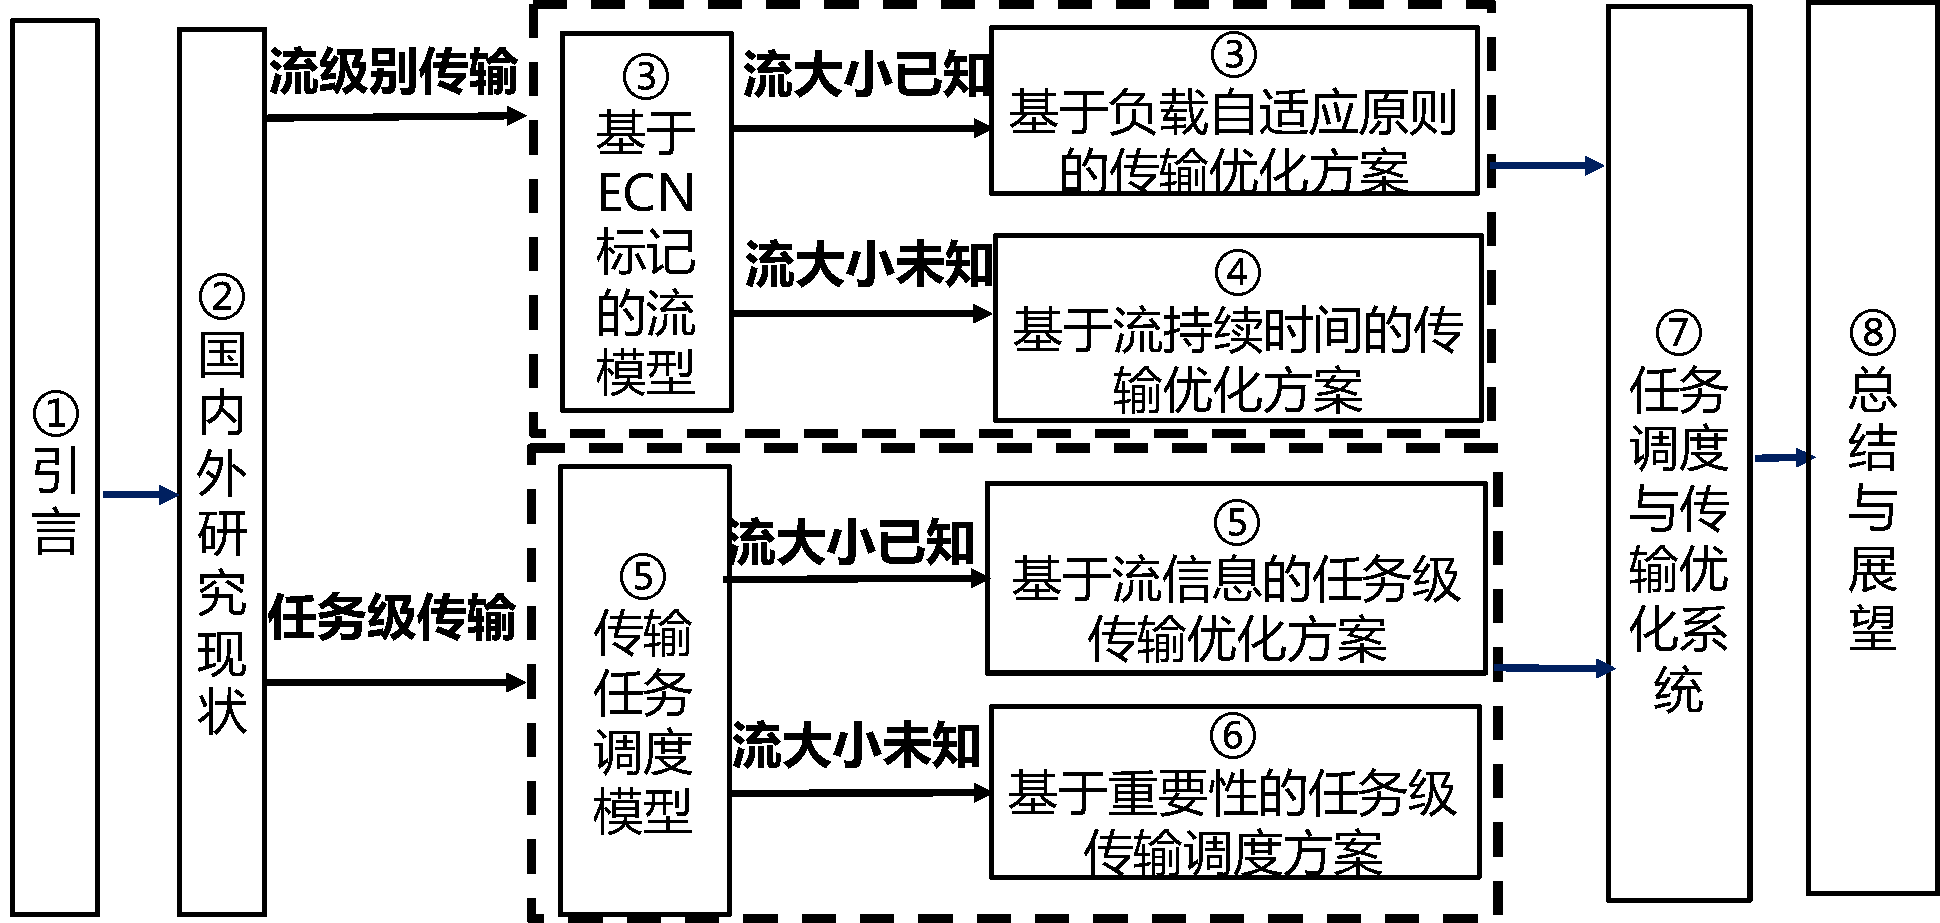
\includegraphics [width=0.9\columnwidth] {figures/structure.pdf}
\caption{论文结构}
\label{paper-structure-fig}
\end{center}
\end{figure}
如图\ref{paper-structure-fig}所示,本文总共分为8章,其中,本章(第1章)是论文引言部分,第2章到第7章是论文的主体部分,
包括流级别的传输优化,任务级别的传输优化和应用传输系统的介绍。
论文的第3章和第4章侧重流级别的传输优化,
第3章介绍了基于 ECN 标记的流模型,
并且提出了基于负载自适应原则的传输优化方案。
第4章介绍了基于流持续时间的传输优化方案。
论文的第5章和第6章介绍的是任务级传输优化方法。
其中第5章介绍了传输任务调度模型,并提出基于流信息的任务级传输优化方案。
第6章介绍了基于重要性的任务级传输调度方案。
第7章主要介绍应用传输系统FlyTransfer以及其性能评测。
第8章是论文的总结部分,主要是对当前工作的总结和对未来工作的展望。



\chapter{相关文献综述}
\label{chapter:background}

\section{本章引言}
本章介绍数据中心应用传输方案的相关工作。
首先,本章从常见应用的通信模型和数据流量等方面对数据中心传输进行概述。
然后,本章从流级别和任务级别对数据中心传输方案进行综述。
最后,本章总结数据中心传输方案存在的问题。


\section{应用传输概述}
在过去的几年中,数据中心随着在线应用的迅速发展取得了巨大的发展。
越来越多的企业有了自己的数据中心,还出现了比如Amazon,微软和谷歌的这些数据中心服务提供商。
在数据中心中有一个持续火热的话题:
如何使用廉价,常见的网络设备来给数据中心应用提供提供低延迟,高带宽服务。
尽管数据中心中存在网络搜索,购物,广告等这些在线应用,这些应用也扮演者不同的角色,
但是,这些应用在使用的通信模型,传输延迟等方面有一些共同的特征。

\subsection{分布式应用的通信模型}

\begin{figure}[h]
  \centering
  \subcaptionbox{Map-reduce}
    {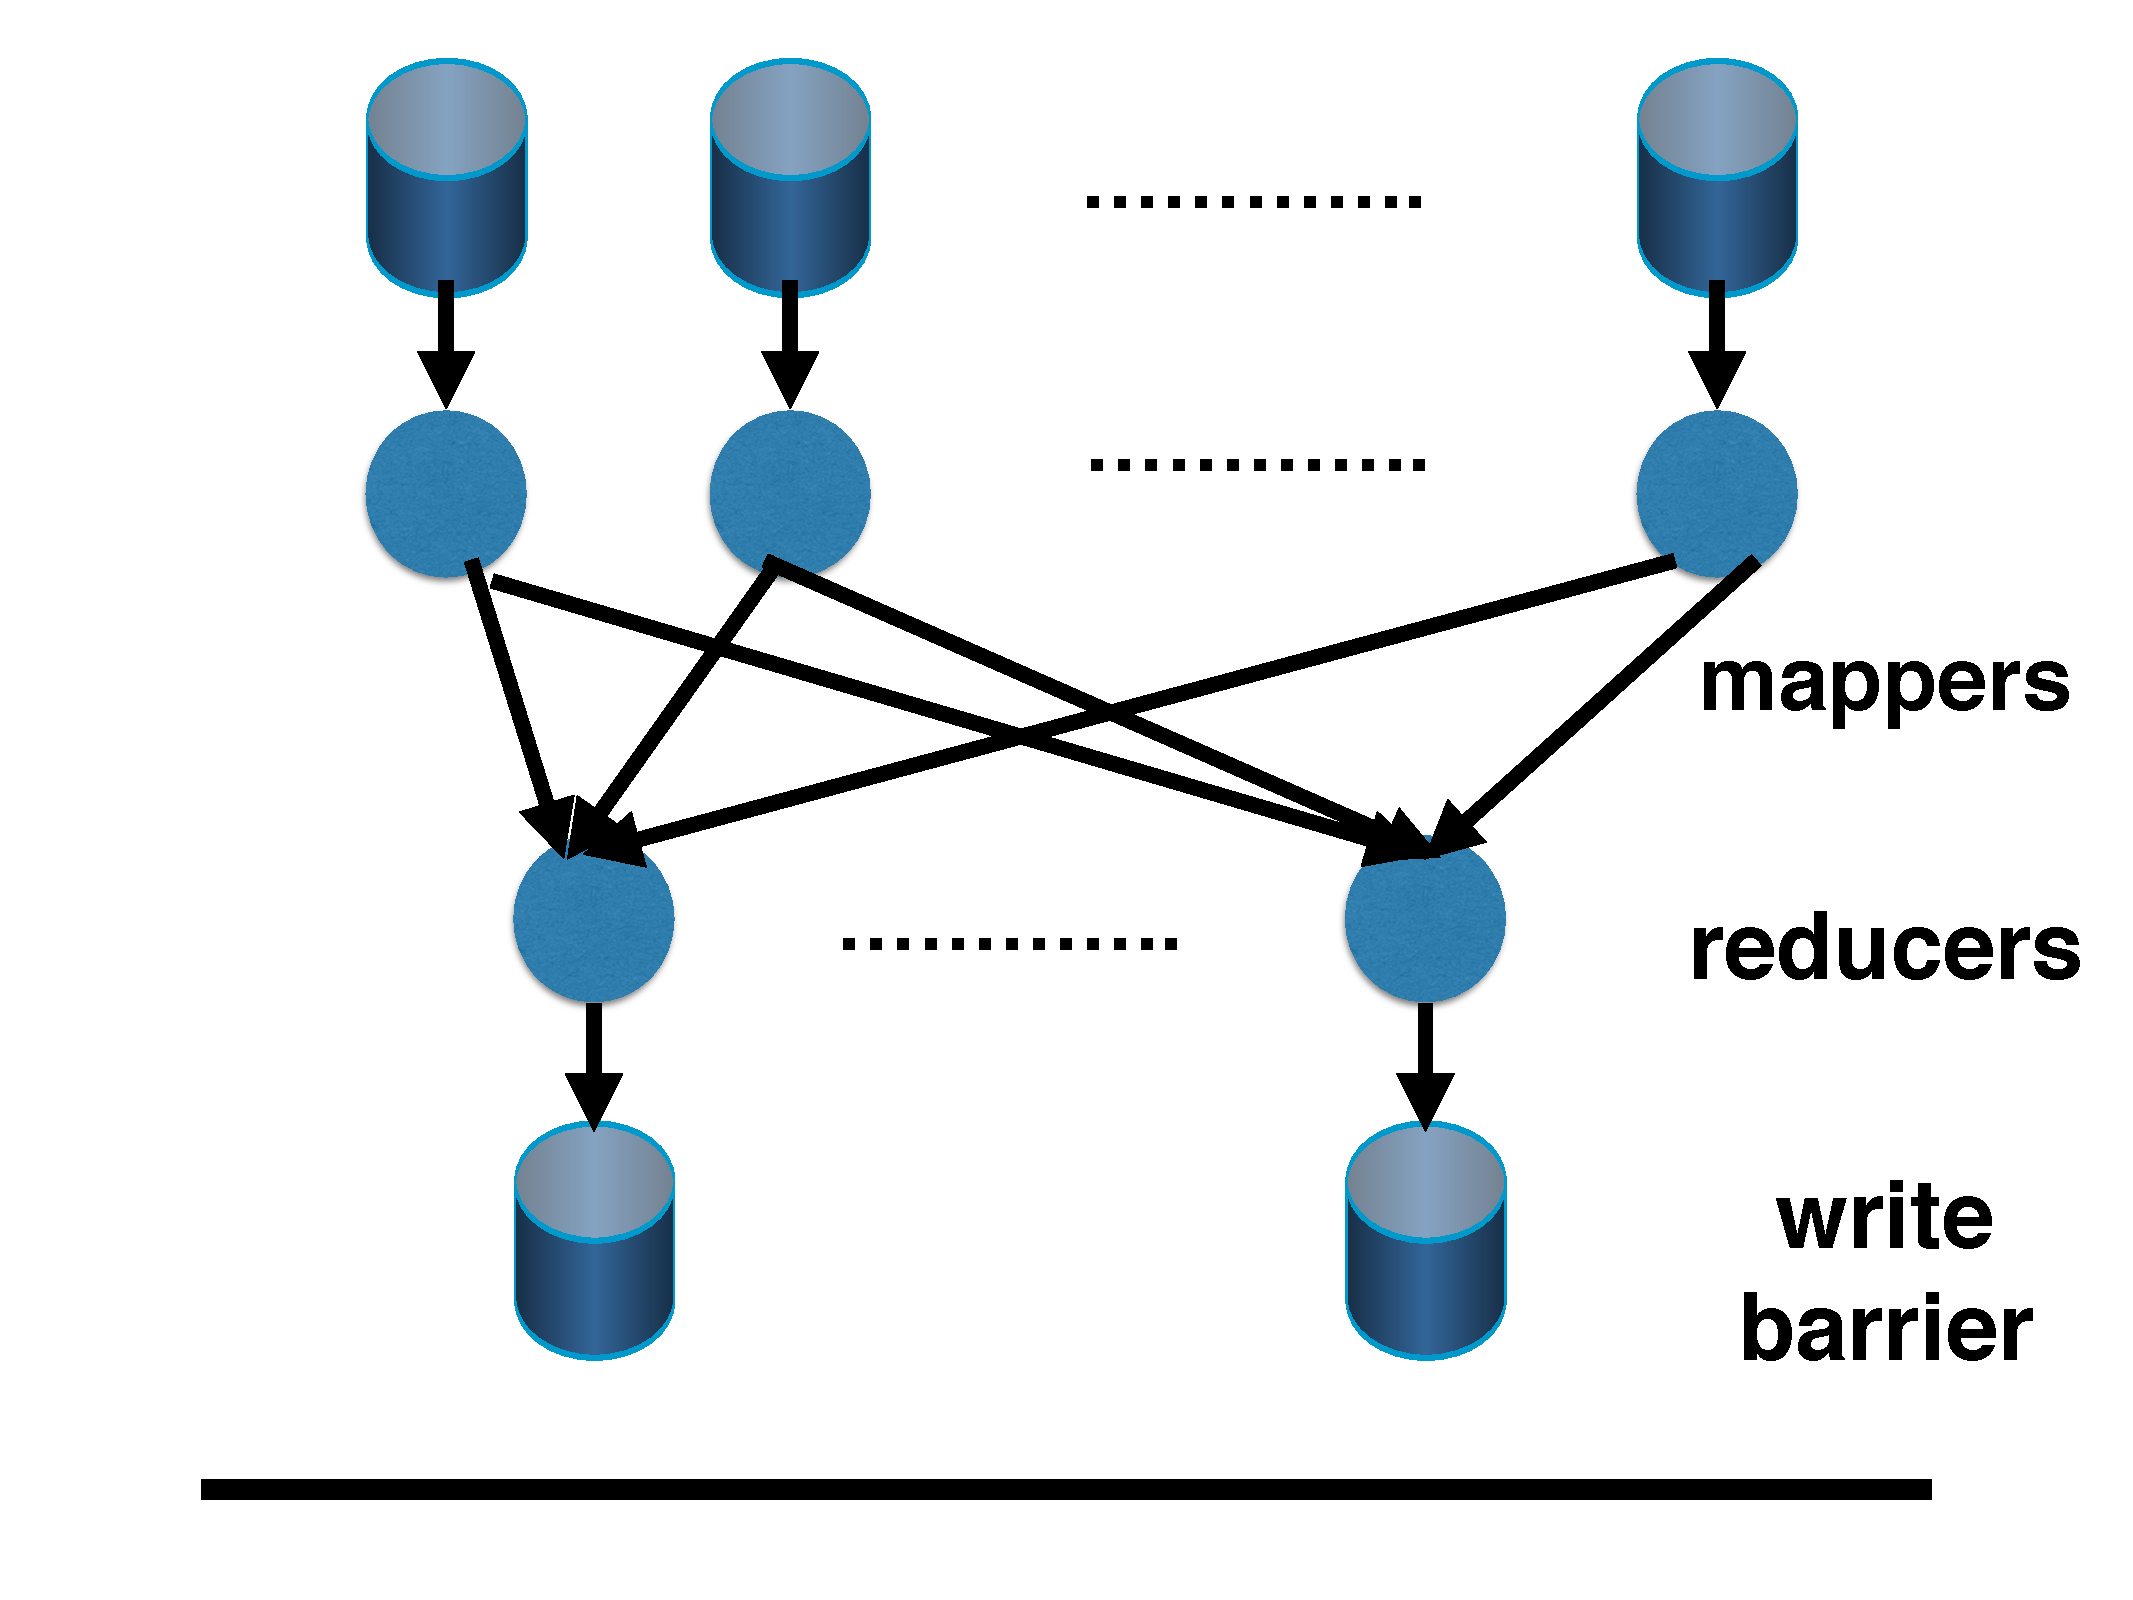
\includegraphics[width=0.48\columnwidth]{figures/others/map-reduce.pdf}}
  \subcaptionbox{带有阻碍的数据流}
      {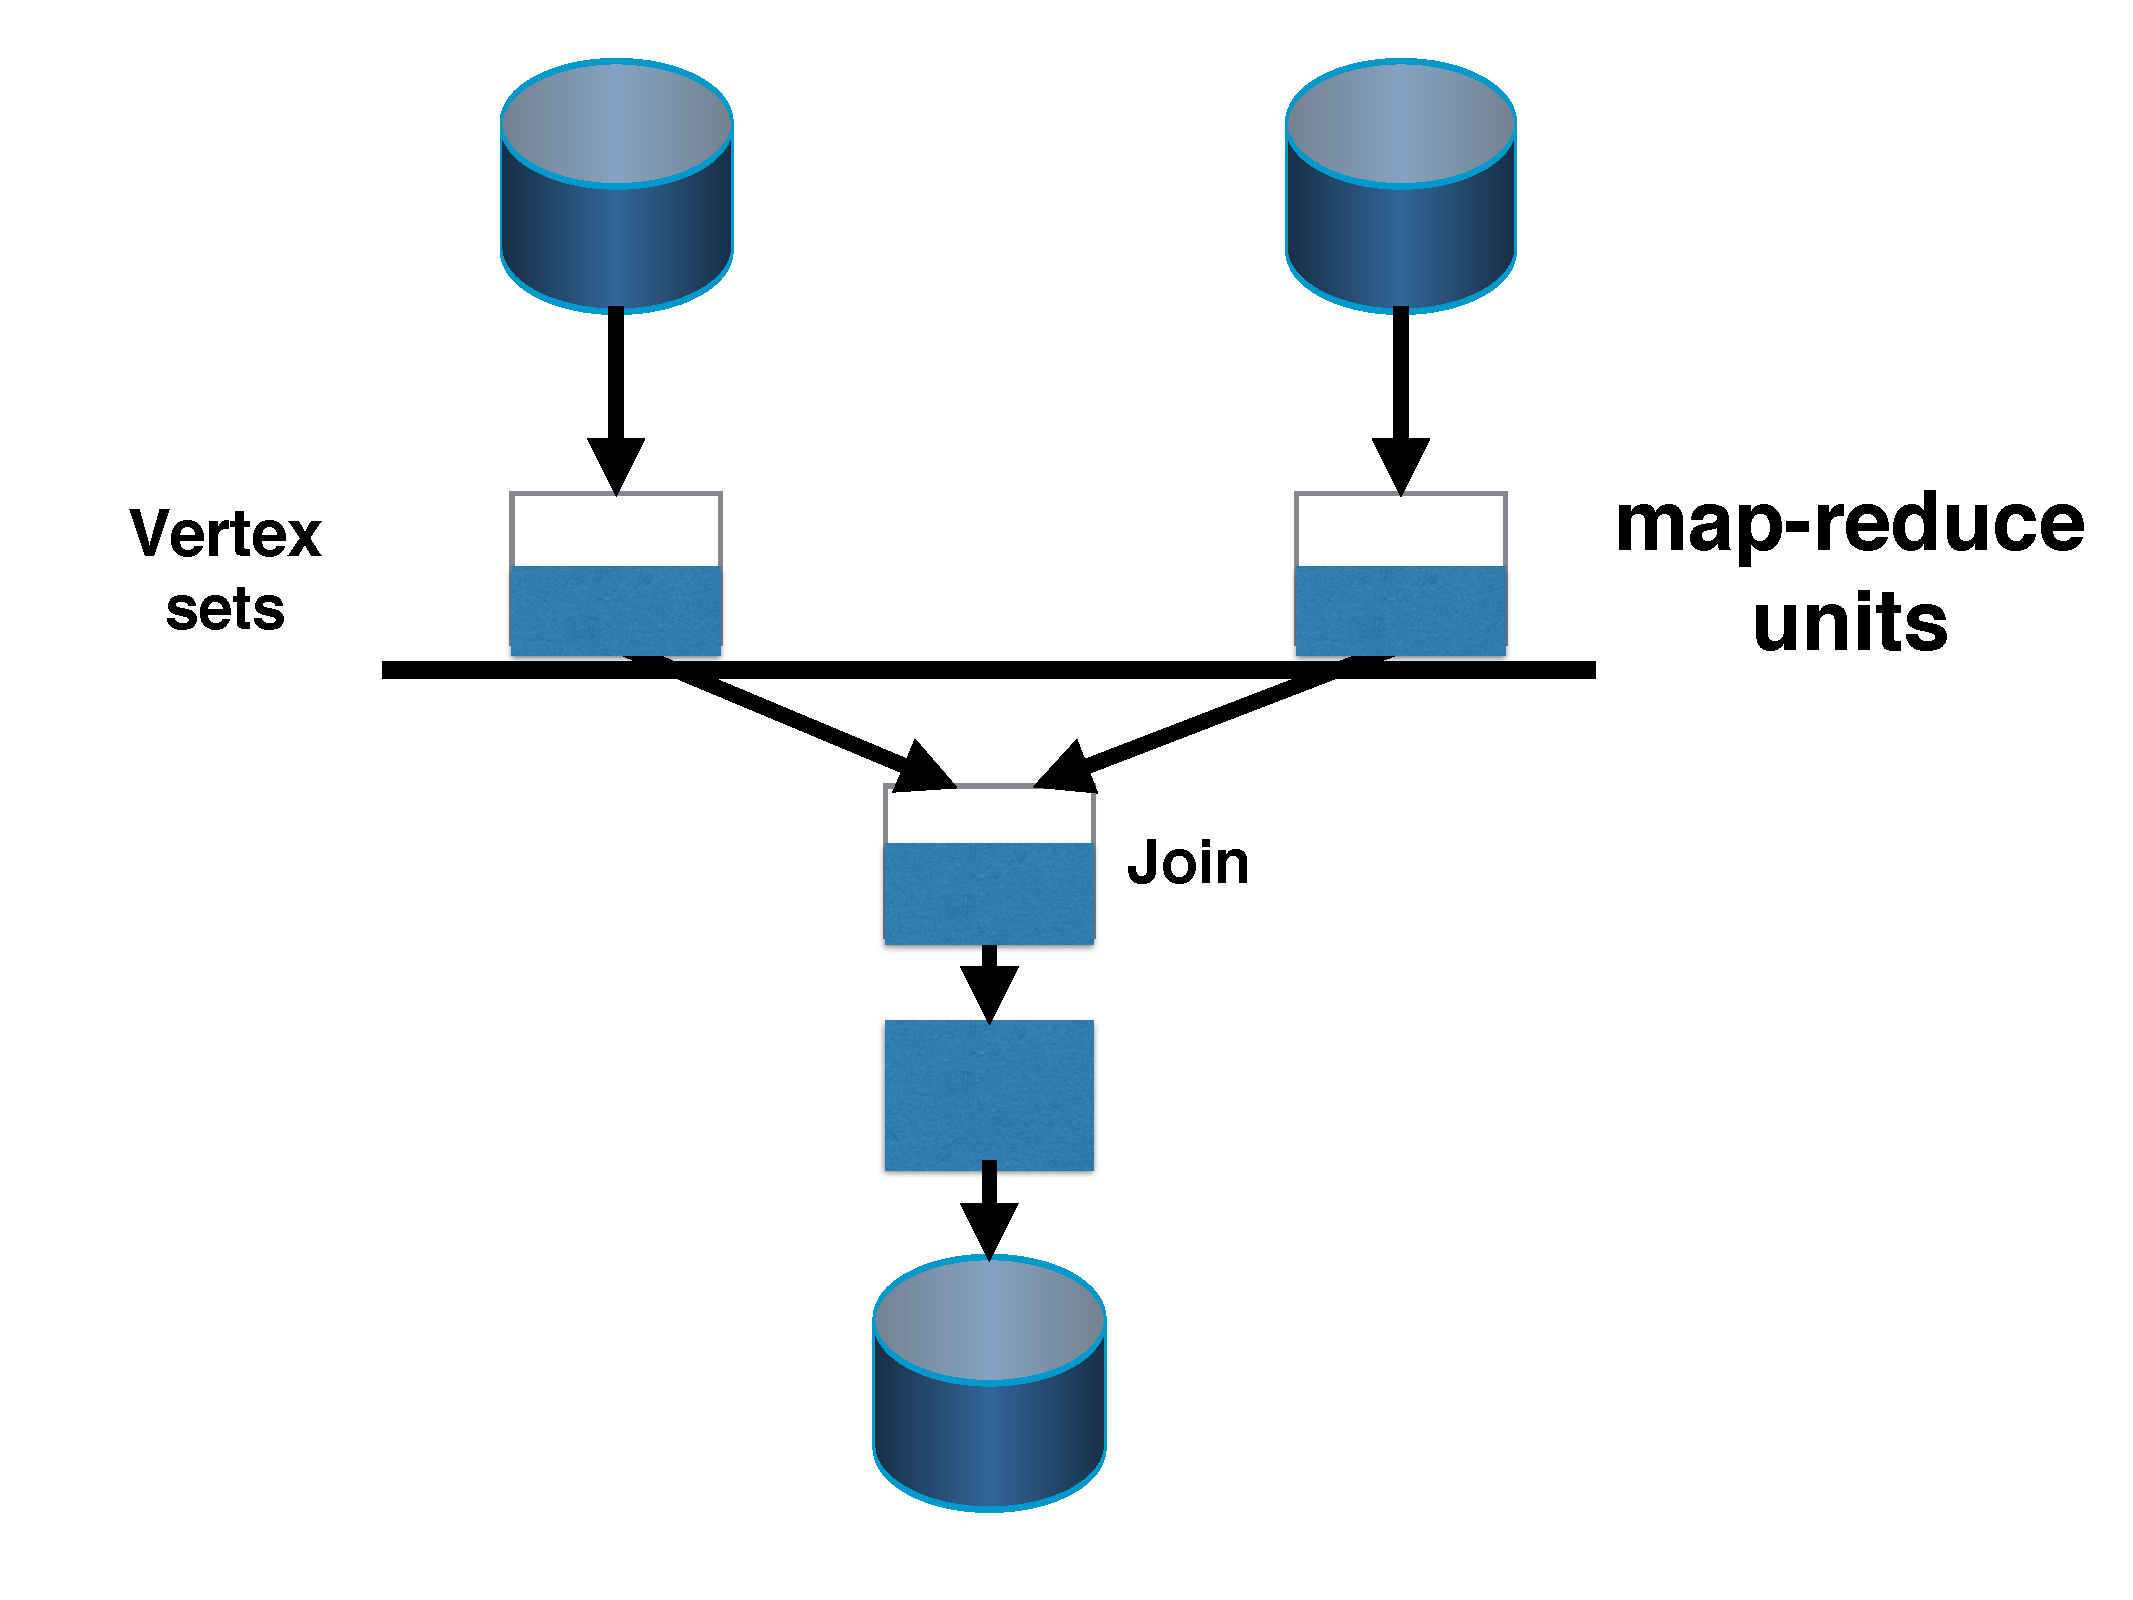
\includegraphics[width=0.48\columnwidth]{figures/others/vertex2.pdf}}
  \subcaptionbox{没有显示阻碍的数据流}
    {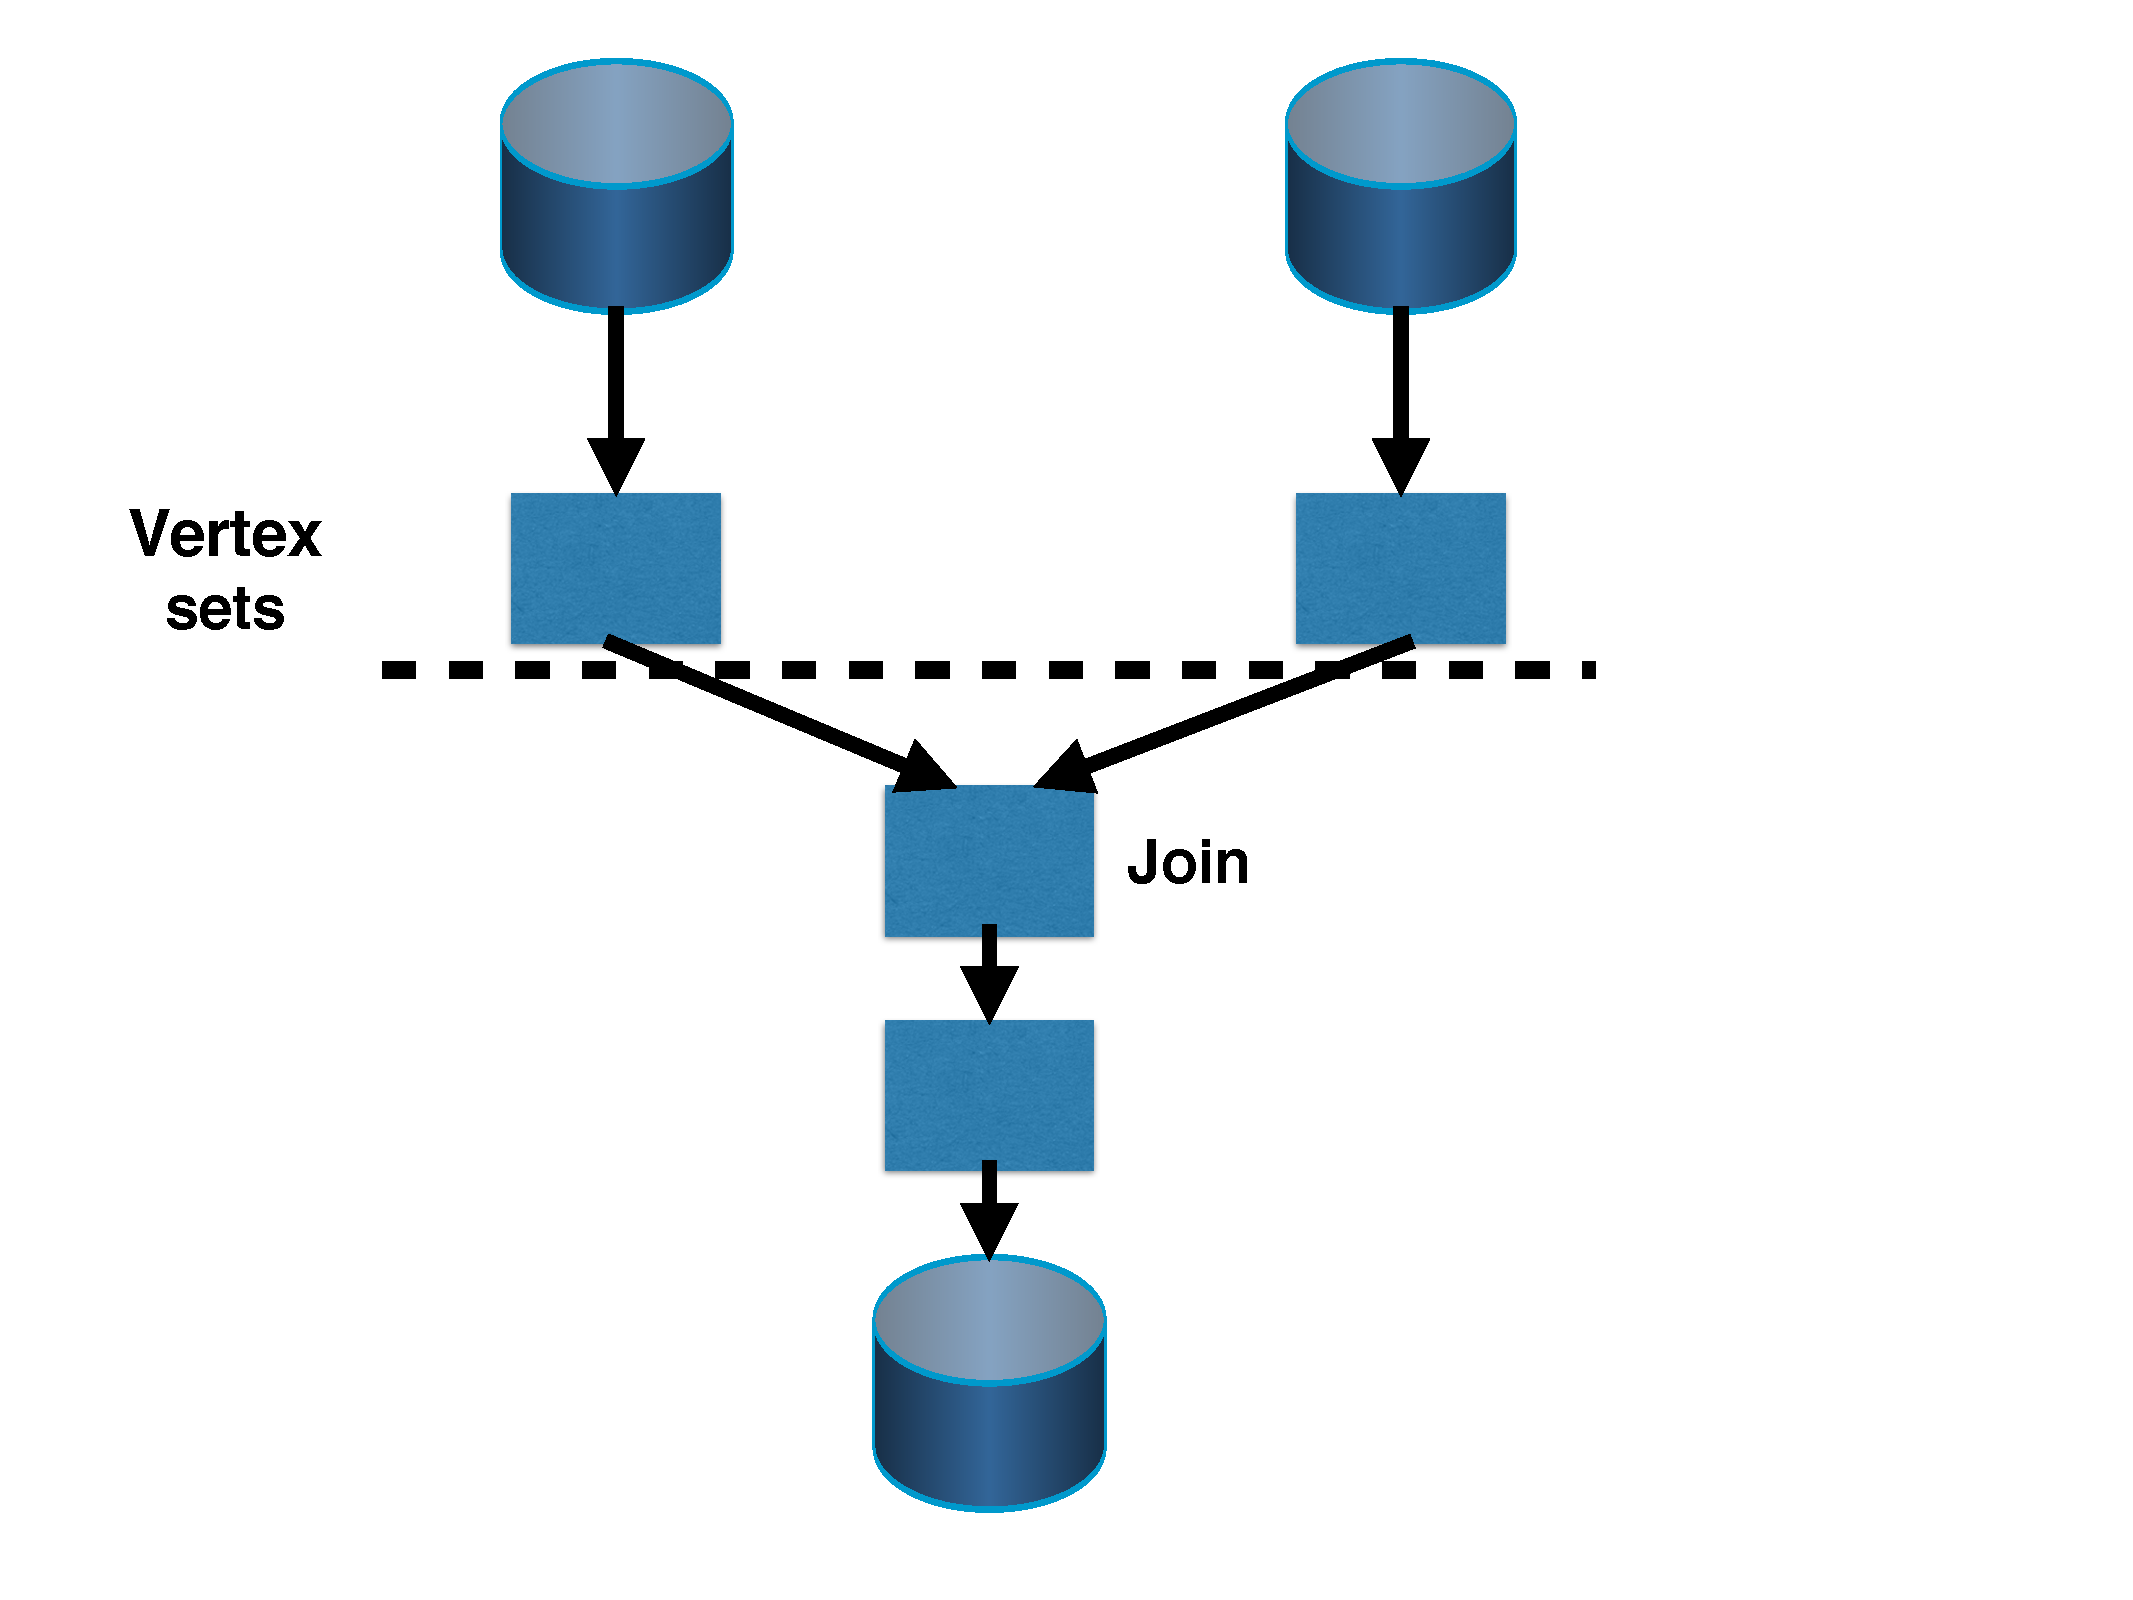
\includegraphics[width=0.48\columnwidth]{figures/others/vertex.pdf}}
  \subcaptionbox{环形数据流}
      {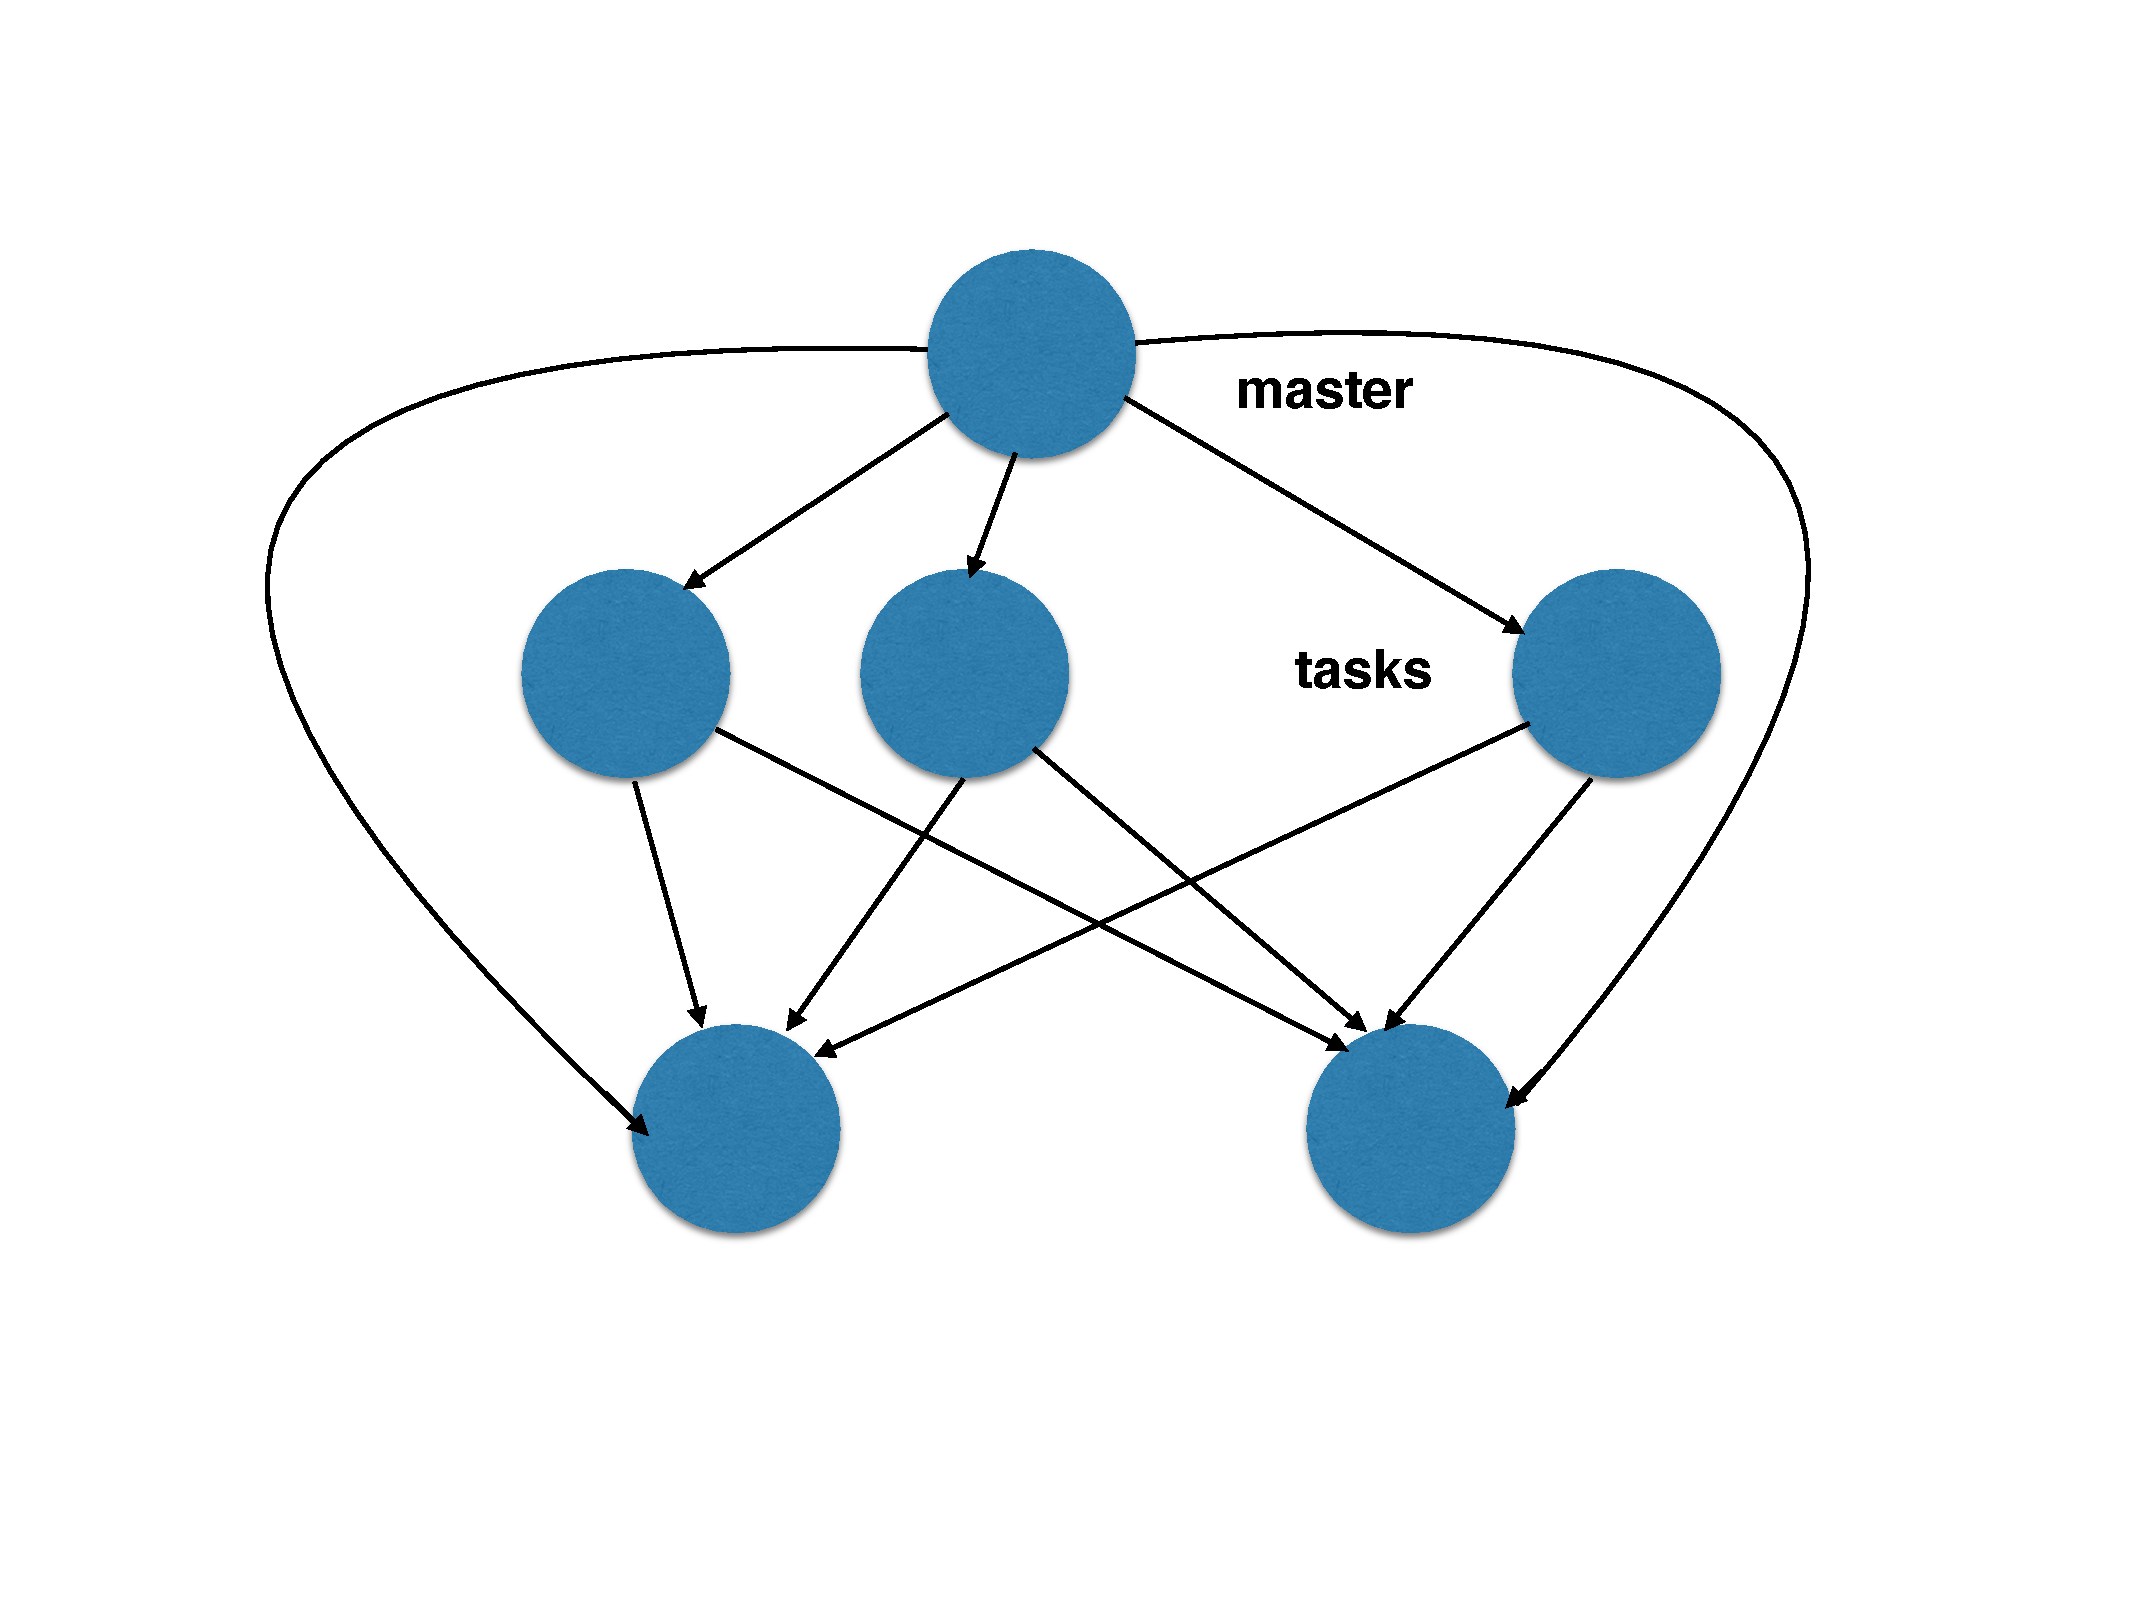
\includegraphics[width=0.48\columnwidth]{figures/others/Dataflow.pdf}}
   \subcaptionbox{并行大块数据流传输}
      {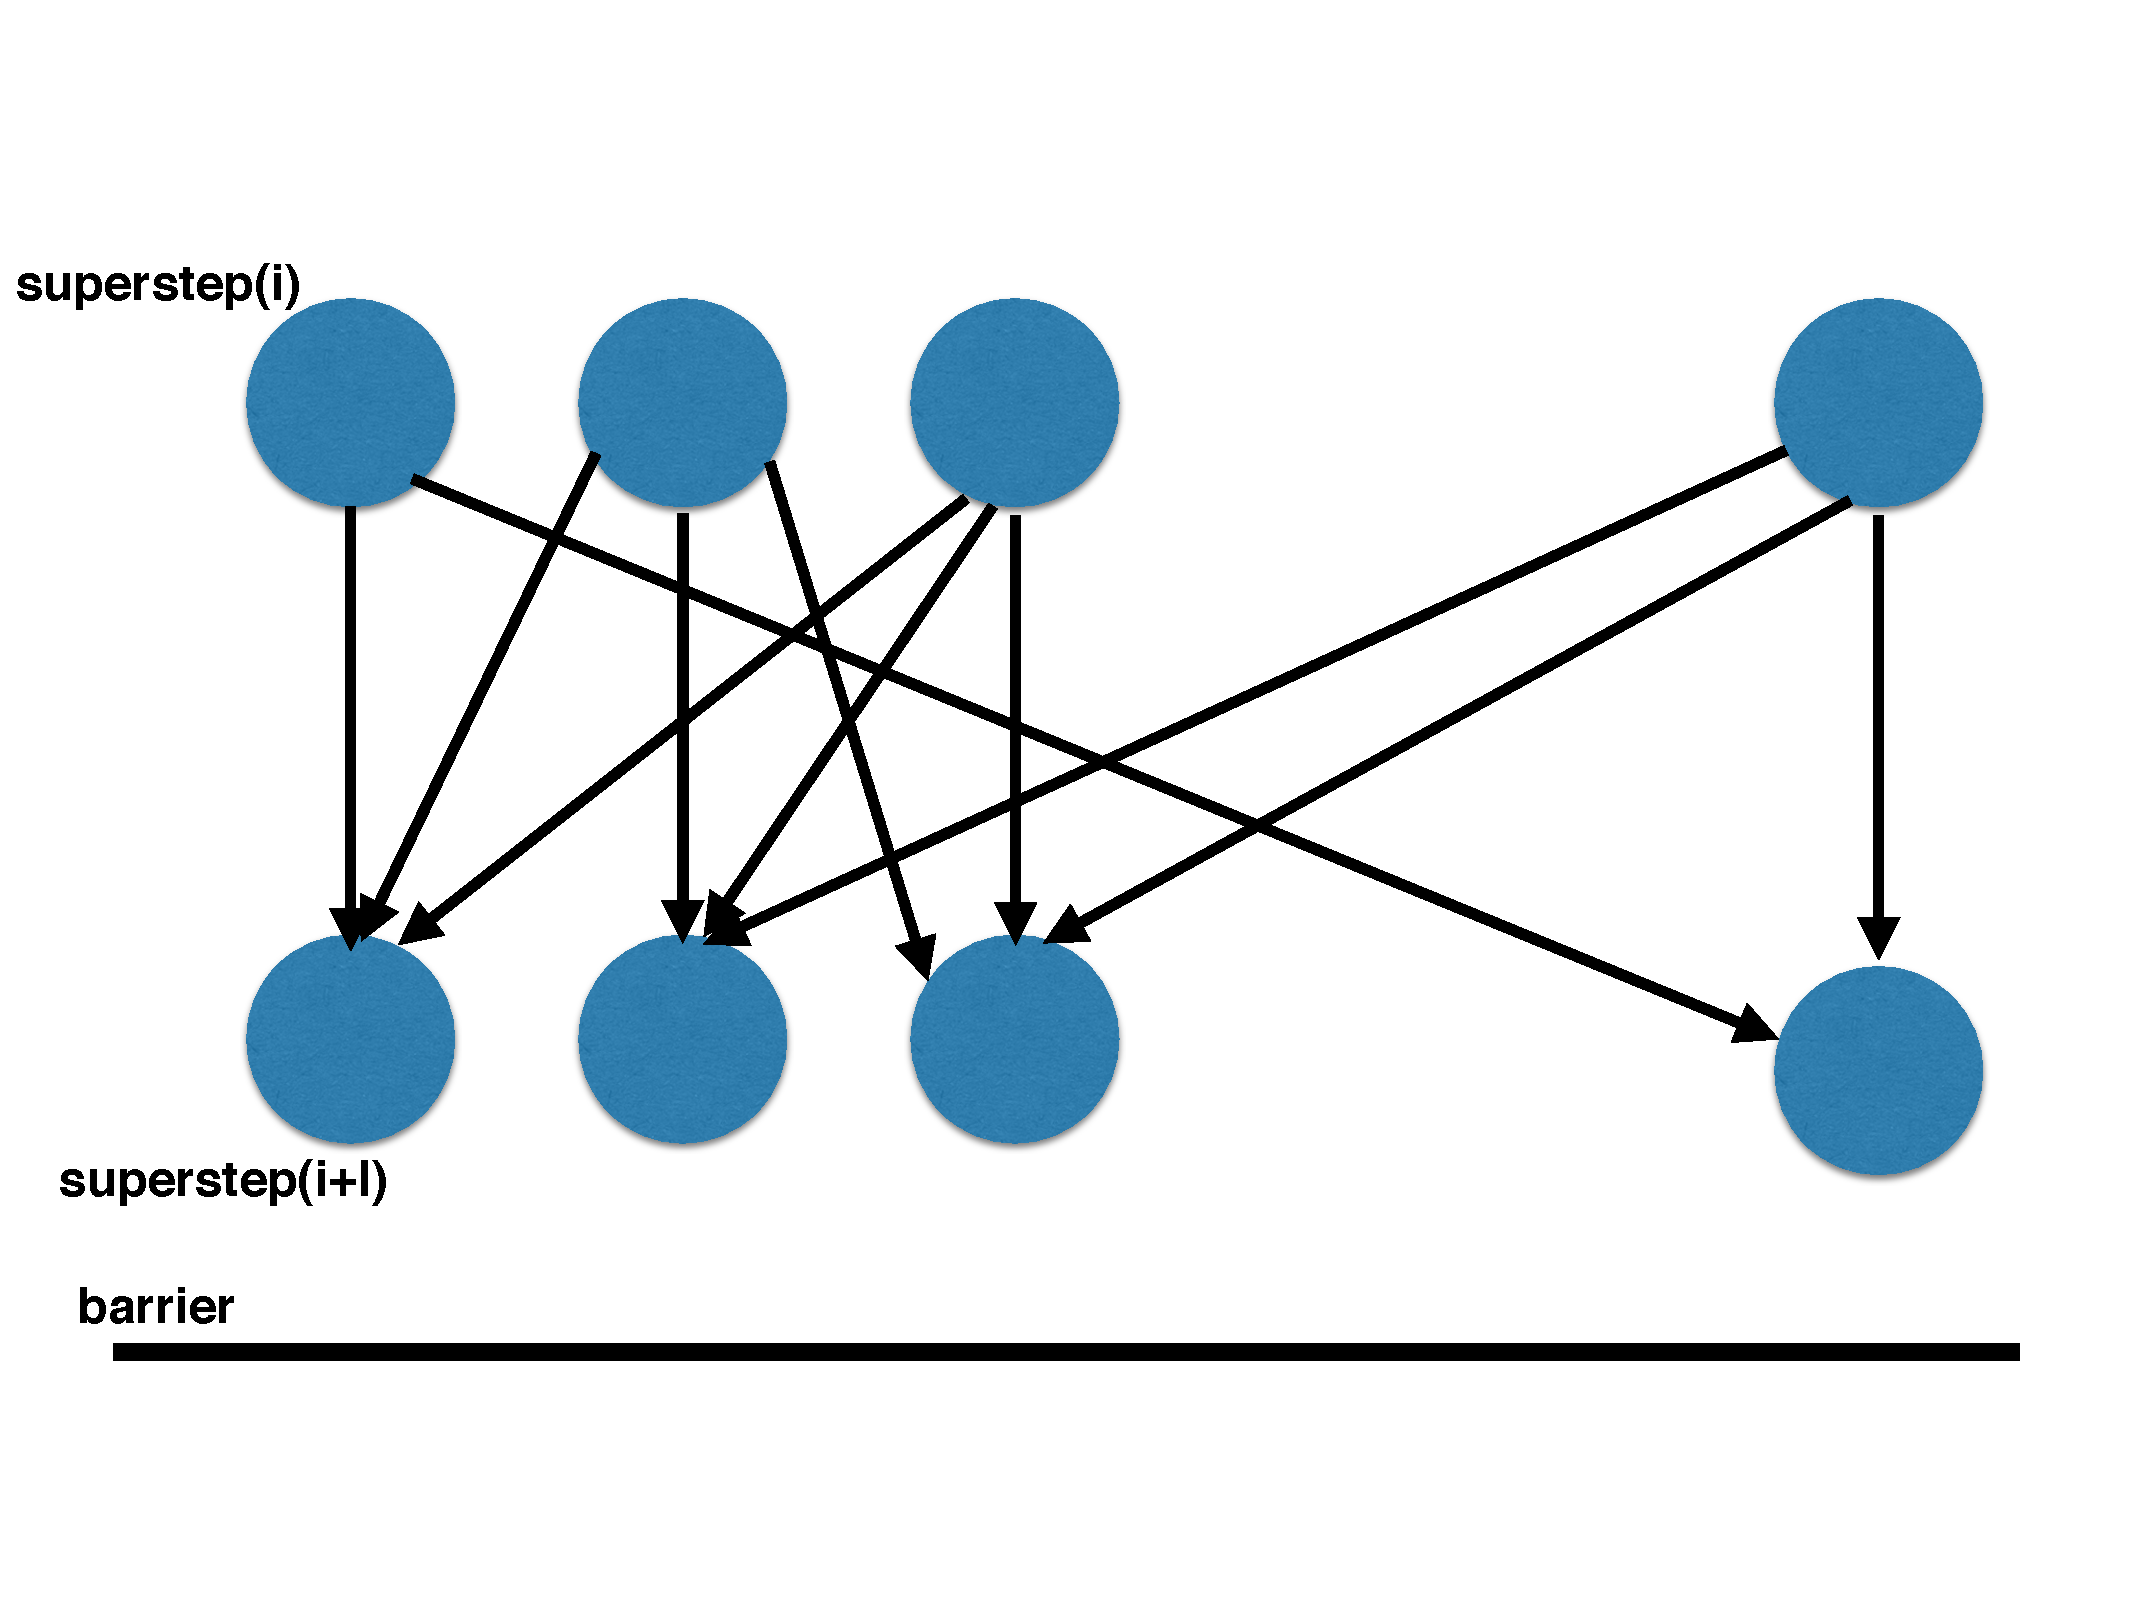
\includegraphics[width=0.48\columnwidth]{figures/others/BSP.pdf}}
   \subcaptionbox{分区-聚合}
      {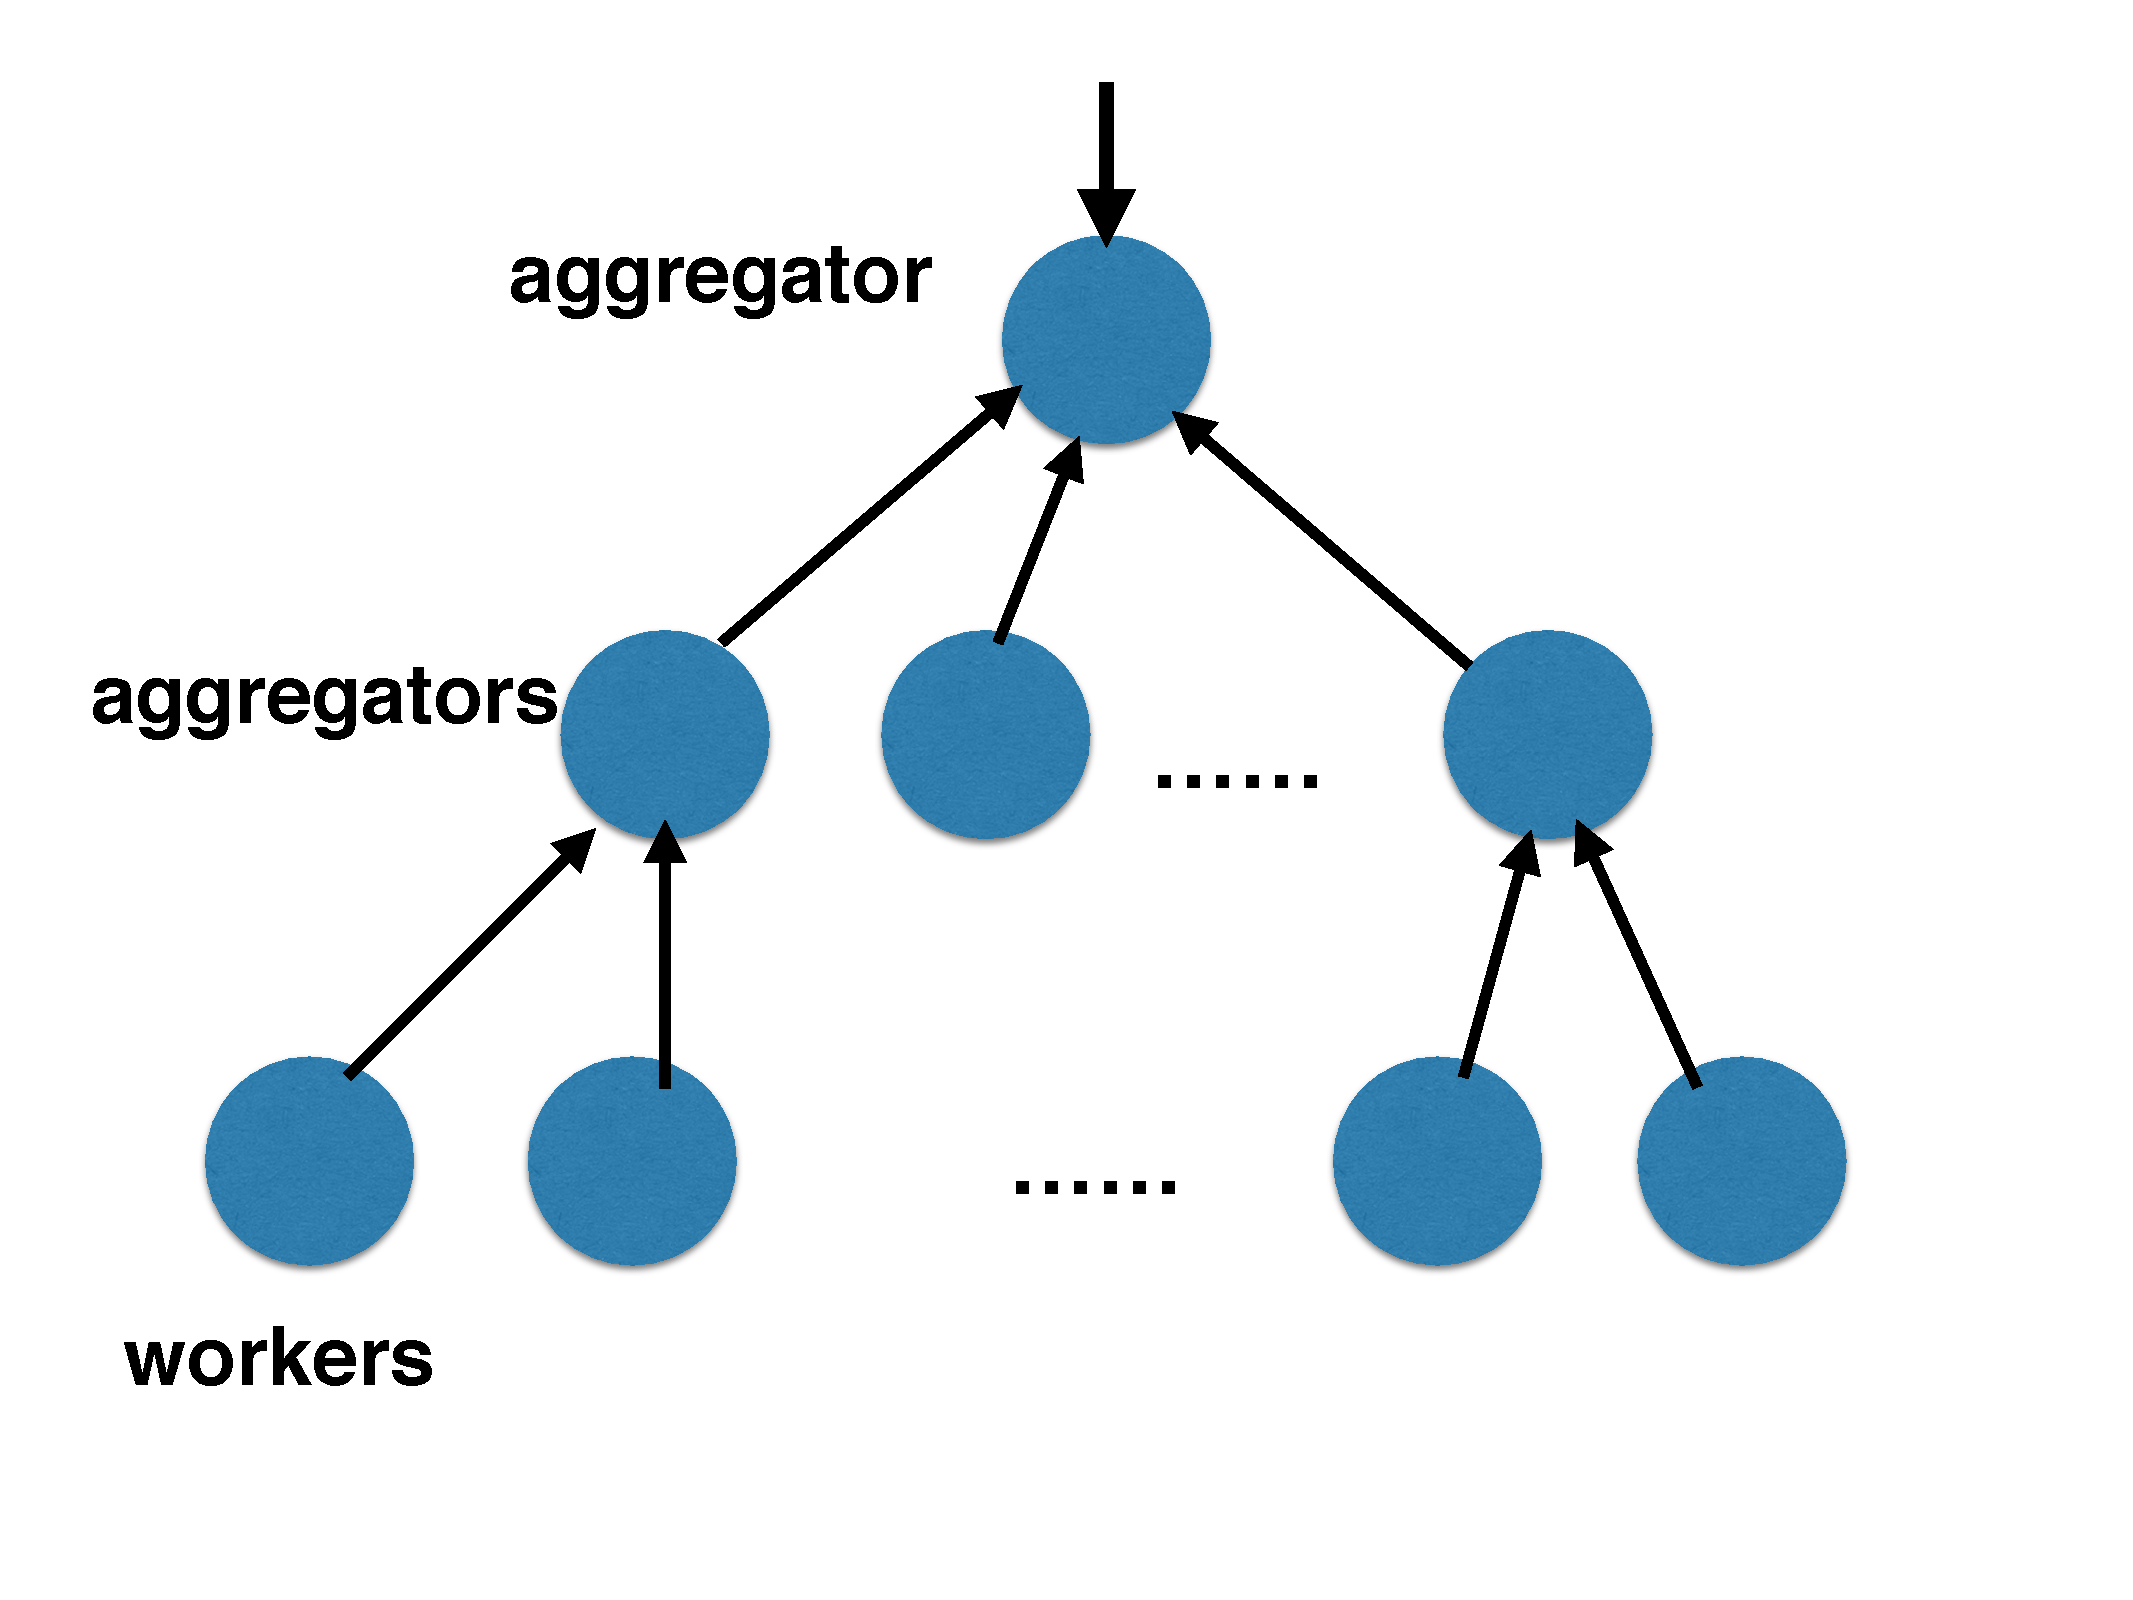
\includegraphics[width=0.48\columnwidth]{figures/others/partition-aggregate.pdf}}
  \caption{分布式应用的通信模型}
  \label{relatedwork-communication-fig}
\end{figure}


大多数集群应用程序的计算框架都是输入特定的配置参数,然后使用特定的计算模型,得到计算结果。
计算过程中,常常产生大量的数据,节点之间会进行频繁通信,不同的计算模型常有不同的通信模式,
这些通信模式可以总结成不同的通信模型。
图\ref{relatedwork-communication-fig}显示了6种通信模型,这些通信模型可以分成4类:
映射规约模型(Map-Reduce),数据流模型(Dataflow),
大型并行数据传输模型(Bulk Synchronous Parallel ),分区-聚合模型(Partition-Aggregate)。

\subsubsection{映射规约模型(Map-Reduce)}
MapReduce\cite{Dean2004Simplified}是一个众所周知的集群计算框架。
如图\ref{relatedwork-communication-fig}(a)所示,
每个mapper都从分布式文件系统(DFS)中读取输入,执行用户定义的计算,并将中间数据写到磁盘上;
每个reducer都从不同的mapper中提取中间数据,将它们合并,并将其输出写入DFS。

给定m个mappers和r个reducer,MapReduce的shuffle阶段将产生总数为$m\times r$条数据流。
经过reducer处理完毕以后,至少有r条数据流被复制。
MapReduce模型中shuffle阶段会产生很多并行的数据流,
直到最后一条数据流传输结束此传输过程才会传输完毕。
因此,在任务传输的最后阶段,有一个显式的同步。
有研究\cite{Chowdhury2011Managing}针对MapReduce存在任务数据流同步的特点,
优化了shuffle阶段的传输,以此来提高传输的性能。

\subsubsection{数据流模型(Dataflow)}
虽然MapReduce被广泛使用,但是因为其存在数据阻塞等问题,常常会影响应用的整体性能。
Dataflow通信模型的出现解决了MapReduce很多的不足,
数据流模型有以下三种方式:

\textbf{带有阻塞的数据流模型}。
如图\ref{relatedwork-communication-fig}(b)所示,
有的多阶段的数据流模型使用MapReduce作为其构建模块(例如,Hive\footnote{Apache Hive.~http://hadoop.apache.org/hive/.},Pig\cite{Olston2008Pig})。
因为基于MapReduce,因此,MapReduce类似,带有阻塞的Dataflow的通信模型在每个构建模块的末尾都有同步操作。

\textbf{无阻塞的数据流模型}。
如图\ref{relatedwork-communication-fig}(c)所示,
一些数据流模型并没有明显的同步操作(比如Dryad\cite{Isard2007Dryad},DryadLINQ\cite{Yu2008DryadLINQ},SCOPE\cite{Chaiken2008SCOPE},FlumeJava\cite{Chambers2010FlumeJava})。
当输入的数据准备好以后,下一个阶段就会开始。
因为没有明确的同步操作,
所以针对MapReduce等存在同步框架的优化技术对此通信框架没有任何效果。
因此,很多研究人员针对采用没有显式阻塞的数据流通信模式的应用进行了特殊优化处理\cite{Guo2015Spotting,Zhang2012Optimizing}。

\textbf{环形数据流模型}。
如图\ref{relatedwork-communication-fig}(d)所示的是环形数据流通信模型。
和无阻塞的数据流模型不同的是,在环形数据流中,数据流会重复使用之前阶段的部分组件。
因为不同的阶段的数据流传输会复用组件,因此,可能会引起组件使用的冲突。
Spark\cite{Zaharia2012Resilient}通过在迭代中保留内存状态来消除循环冲突带来的开销。

\subsubsection{大型并行数据传输模型(Bulk Synchronous Parallel )}
大型并行数据传输模型(Bulk Synchronous Parallel,简称BSP )是集群计算中的另一个众所周知的通信模型。
使用这种模型的框架包括Pregel\cite{Malewicz2010Pregel}、
Giraph\footnote{Apache Giraph.~http://incubator.apache.org/giraph/.}和Hama\footnote{Apache Hama.~http://hama.apache.org.}等,
许多图形处理、矩阵计算等工具使用BSP框架。
如图\ref{relatedwork-communication-fig}(e)所示,
BSP计算在一系列全局superstep中进行,
每个superstep包含三个有序阶段:并行计算、进程通信和同步数据。
在每一个superstep的末尾有明确的同步操作。

\subsubsection{分区-聚合模型(Partition-Aggregate)}
图\ref{relatedwork-communication-fig}(f)显示是数据中心分区-聚合模型(Partition-Aggregate)。
分区-聚合模型是很多大型分布式计算通信模型。
在分区-聚合模型中,请求发送到根节点,根节点把请求下发给底部的worker节点。
随后,worker节点把结果聚集到一起,然后把计算完成的结果,反馈给根节点。
在数据中心,网络搜索、社交网络内容组成和广告选择等应用的通信模式均是基于此模式设计的。
对于交互式的、实时的应用,用户得到响应的延迟是衡量服务质量好坏的重要指标。
在减去传输等延迟之后,留给计算的时间通常只有230$\sim$300毫秒。

许多应用采用多层的分区-聚合模式,其中一个层的传输延迟会影响另一个层的启动。
此外,响应请求可能需要迭代地调用,一个aggregator节点向下面的worker节点发出连续的请求,
以准备响应(1到4次响应是常见的,甚至有时能到20次)。
例如,在web搜索中,一个查询会发送给许多aggregator和worker,每个组件负责不同的部分。
根据回复,聚合器可能会细化查询并再次发送,以增加结果的完备性。
因此,分区-聚合传输延迟过高会增加对查询结果性能的影响。


为了防止SLA(Service Level Agreement)性能被破坏,
常常需要给worker节点设置一个截止期限(deadline),截止期限通常在10ms$\sim$100ms。
当一个worker节点错过了截止期限时,上层aggregator节点将会收到不完整的结果,这样会使的计算结果受到影响。
因此,对于用户来说,越来越多的的流在截止期限之前完成对用户体验十分重要。
例如,可能有$99.9\%$的流在截止期限之前完成,意味着,1000个请求中,有1个请求不能在截止时间之前完成。
这样会严重影响用户的体验,造成客户的流失,造成不可逆转的损失。

\subsection{网络流量特征分析}

随着数据中心中部署应用的增多,对数据中心中流量特性的研究也逐渐增多。
本部分对当前业界对数据中心流量测量的工作进行了总结和归纳。




\textbf{查询流}。查询流常常是由类似web这类请求产生的,这种请求的通信模型常常是Partition-Aggregage。
查询流非常短,并且对延迟十分敏感。
当一个用户请求到达上层aggregator的节点时,上层的网络节点把请求下发给中层的节点,计算结果后,然后再下发给下层的worker节点。
worker节点得到请求后,读取请求的内容,然后计算结果,
随后把结果反馈给根节点,根节点根据得到的反馈结果,进行处理。
查询流的规模是非常有规律的,从高层的根节点到下层的worker节点的查询流的大小约为1.6KB,
从子节点回馈给根节点的流大小大约是1.6KB到2KB。





\textbf{背景流}。背景流和查询流共同存在于数据中心。
大多数背景流通常短于1MB,但是数据中心超过$90\%$的数据量来自约$1\%$的背景流。
这些长流通常在1MB到50MB之间。
在分布式模型中,有很多拷贝和更新节点状态的背景数据流,这些流大小在50KB到1MB。
背景流的到达间隔时间反映了应用的不同服务的叠加和应用的多样性。
背景流有如下的特性:
(1)流到达时间间隔跨度很大,流的到达是服从重尾分布,在较短的时间间隔内,会有大量背景数据流到达。
(2)长流发送是有一定周期性的,出现周期性是因为下层的叶节点会周期性的更新文件,此过程中会产生大量流。





\textbf{数据流并行程度和大小}。
在数据中心内,并行流数目的中位数为36。
$99\%$的机器之间连接数目在1600以内,有的机器连接的中位数,甚至在1200\cite{DCTCP}。
当只考虑长流($>$1MB时),机器之间并发的长流数目较少,并行的长流的平均数为1,
并且大约$75\%$的机器长流的并发数目在2以内。
这些流,能持续几个RTT,交换机的缓冲区大部分空间都是由这些流的数据包占据。

总之,对延迟敏感的查询流和需要高带宽的背景流同时存在于数据中心,
在数据中心,这些数据流对网络资源的需求不同,
我们需要设计合理的网络协议,来满足不同的流对网络资源的需求。

\textbf{关于期限}。Web应用的交互性意味着延迟是决定服务质量的关键。
研究表明,用户需要快速的回复响应\cite{kohavi2009controlled}。
除去节点之间网络传输时间,
应用通常具有200$\sim$300ms时间以完成其操作并对用户进行回复\cite{Decandia2007Dynamo}。

\begin{figure}[b]
\begin{center}
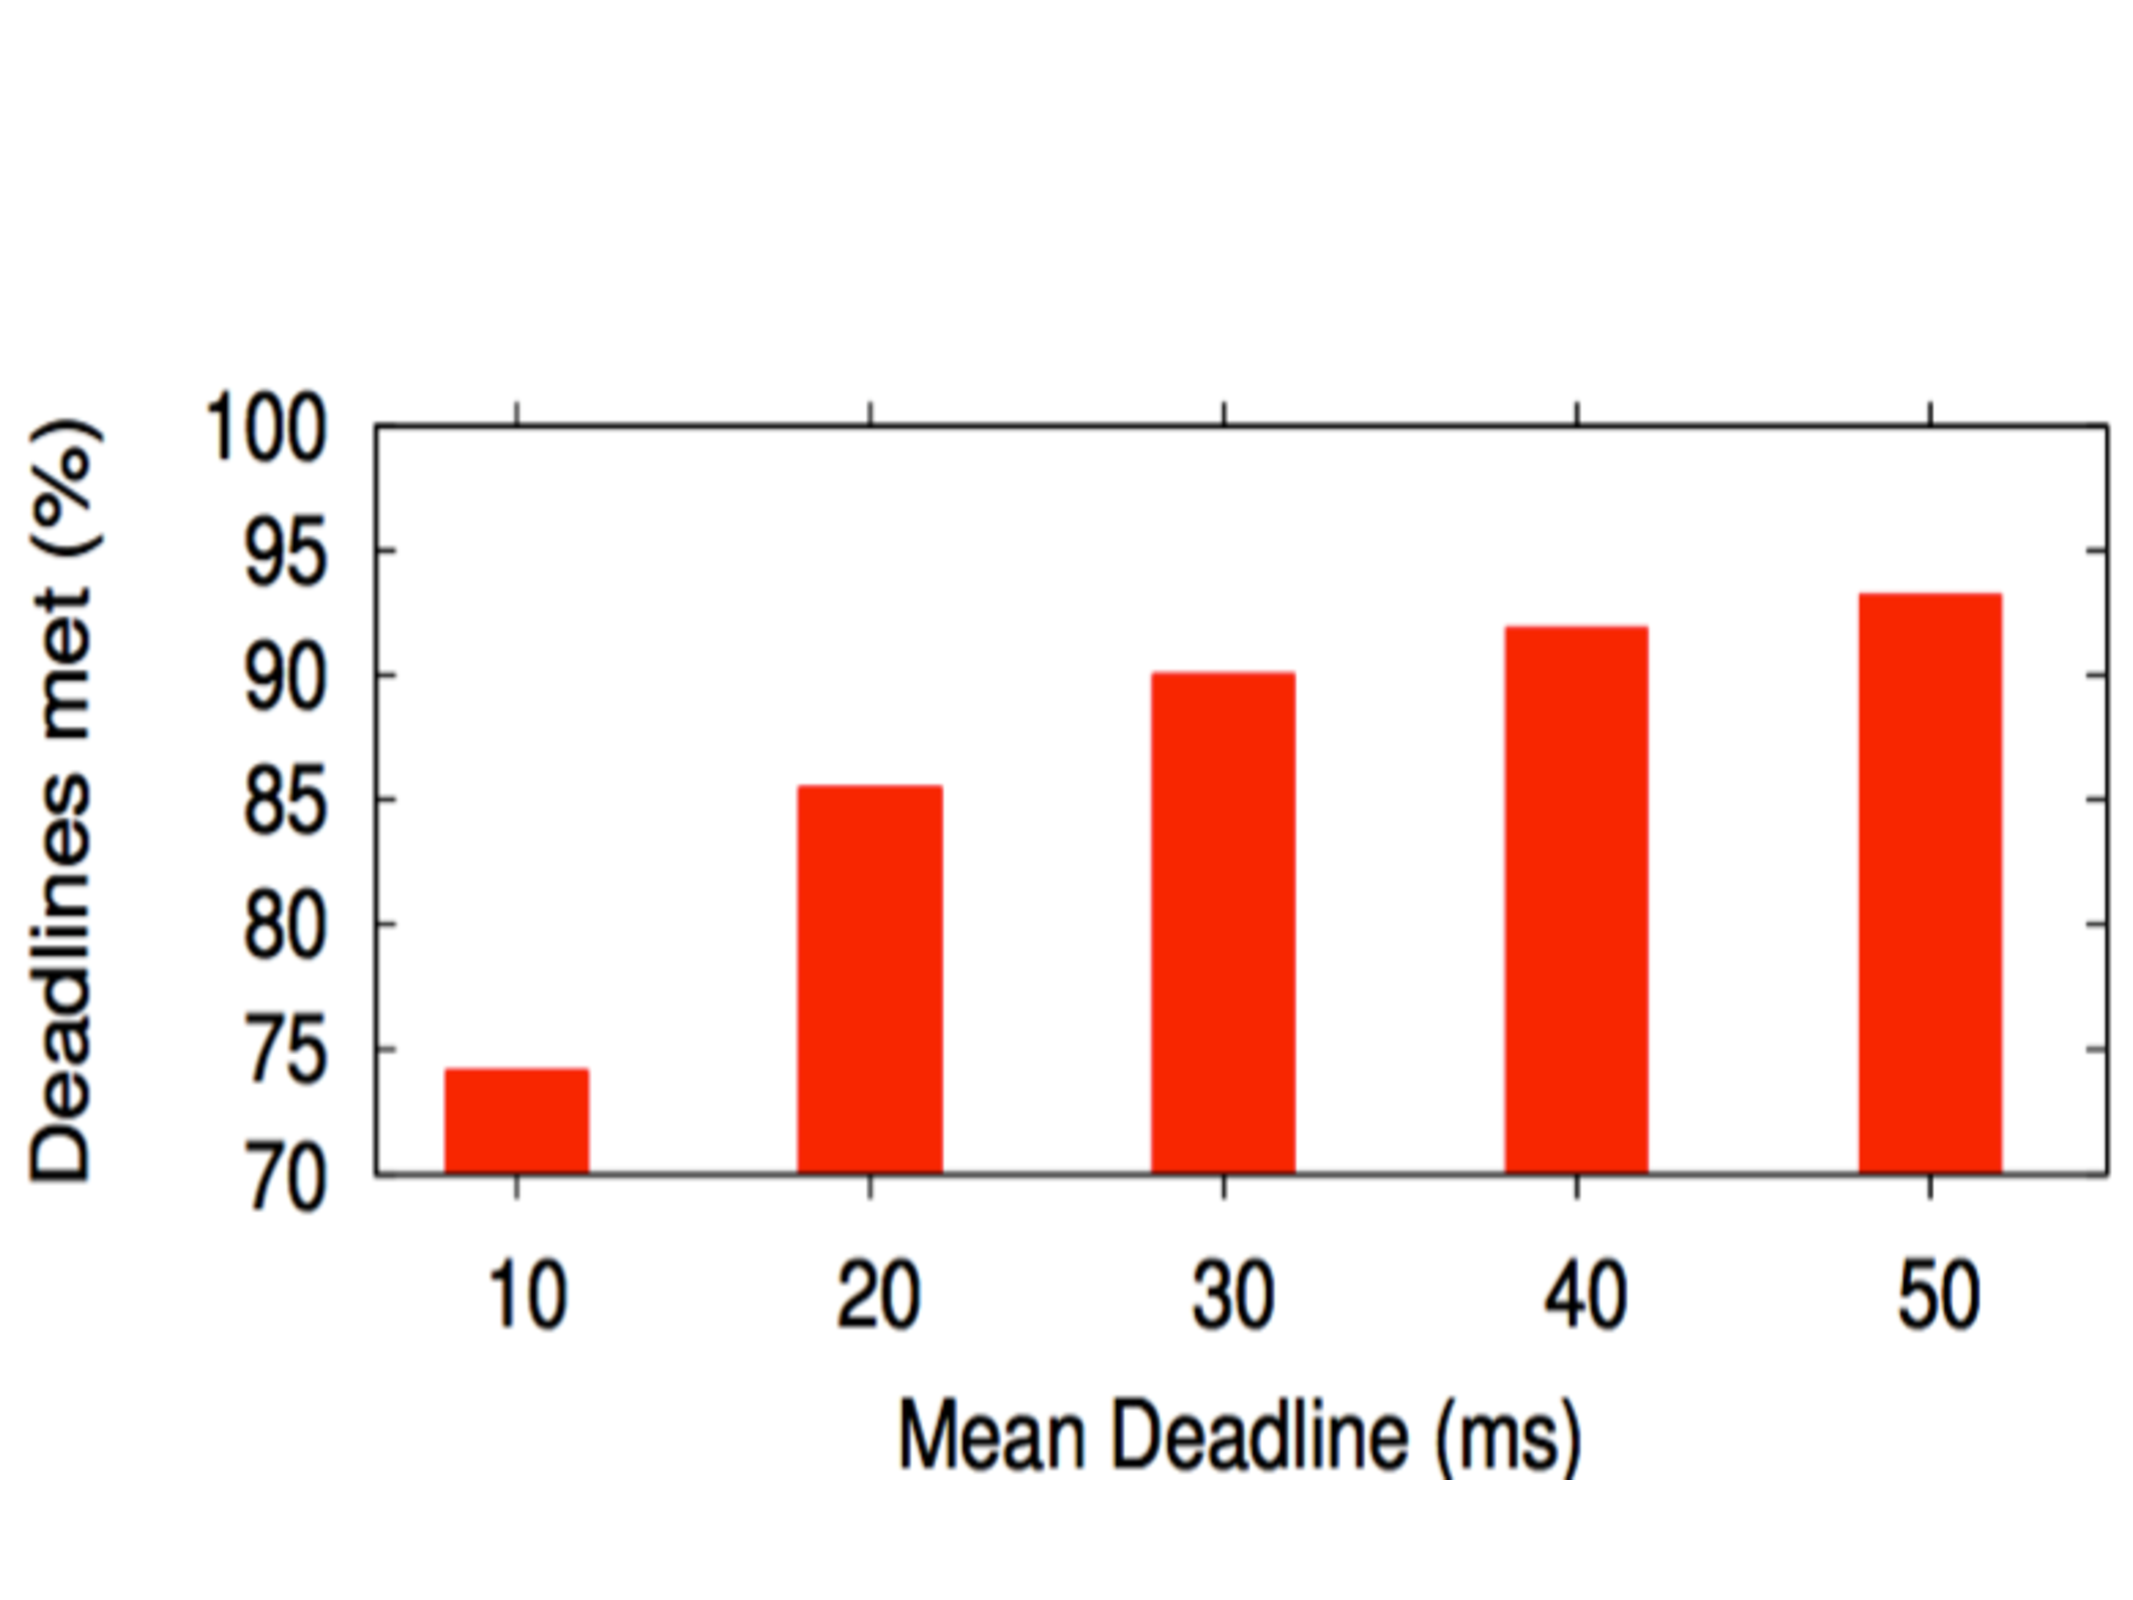
\includegraphics [width=0.9\columnwidth] {figures/others/deadline-picture.pdf}
\caption{partition-aggregate 模型}
\label{relatedwork-deadline-fig}
\end{center}
\end{figure}

因此,诸如Partition-Aggregate这类模型的SLA (Service Level Agreement)
要求worker等节点的询问和应答传输在截止期限(deadline)之前完成。
任何没有在截止期限之前完成的数据流都被认定错失期限。
错失期限的数据流越多,会有越多的上层计算节点获得不完整的结果,进而影响服务的质量。
此外,在实际中不同的应用的数据流有不同的截止期限,甚至,同一个应用的不同阶段的传输的期限也不相同。
在实际中,数据中心的流包括时间敏感的短消息(50KB到1MB),用于更新节点状态和传输时间长的背景流量(5KB到50MB)等。
这些数据流在节点之间传递,不同业务的数据流具有不同的期限,有的甚至没有期限。
图\ref{relatedwork-deadline-fig}显示的流传输期限分布情形,从中发现,超过$90\%$的数据流的期限在50ms以内。
事实上,数据中心很多在线服务都需要性能保障\cite{Decandia2007Dynamo,Renesse2002Scalable}。
用户的请求,需要满足延迟的需求。
当请求到达时间节点时,
无论计算结果如何,节点都需要把结果反馈给用户,
如果错过了截止期限,应用的性能难以得到保障。



\subsection{TCP传输存在的问题}
TCP是一种面向连接的、可靠的、基于字节流的传输层通信协议。
尽管TCP在Internet中被广泛应用,然而数据中心应用常常需要数据中心网络提供低延迟高带宽。
因为数据中心网络资源有限,因此直接在数据中心使用TCP协议,会存在以下问题。

\subsubsection{Incast问题}
如果很多数据流在短时间内收敛在交换机的同一接口上,数据包可能会耗尽交换机的缓冲区,导致数据包丢失,导致Incast问题\cite{Vasudevan2009Safe}。
发生Incast常常是因为应用采取分区-聚合通信模式,因为在分区-聚合通信模式中,
工作节点常常在较短时间间隔内会发送反馈给上层节点,导致上层节点交换机缓冲区溢出。

迄今为止的实验发现,Incast经常会发生在实际生产环境中,Incast会影响用户体验,从而影响企业的效益。
这是因为,Incast会导致交换机缓冲区过大,从而请求的数据流错过期限。
如果使用TCP协议,则解决Incast问题的方法主要有:
(1)为每个请求增加随机抖动时间。
使用增加抖动时间的方法,可以避免Incast问题,
但是,给每条流增加随机的抖动,会使一些短流增加额外的延迟,从而使数据流错过期限;
(2)把数据流拆分成短流来适应交换机的缓冲区。
使用拆分数据流的方法,会从语意上破坏应用的完整性。
如果某条短流丢弃数据包,会使的整条长流传输不完整,从而破坏应用的性能,进而影响用户的体验。

\subsubsection{交换机缓冲区队列过长}

大多数数据中心的交换机是共享内存,
交换机的所有端口共享交换机存储。
到达交换机接口的数据包被存储到所有接口共享的高速存储器中。
共享池中的内存由内存管理单元动态分配给数据包。
内存管理单元尝试为每个接口分配尽可能多的内存,
如果一个数据包必须排队等待出端口,
但接口已经达到了最大内存分配或者共享池本身已经耗尽,那么数据包就会被丢弃。
构建大型多端口存储器非常昂贵,
所以大多数便宜的交换机都是缓存都很小。

当前计算机网络判断拥塞的方法主要有三种:基于丢包的拥塞控制方法,基于RTT的拥塞控制方法,基于交换机队列长度的拥塞控制方法。
TCP使用基于丢包的拥塞控制方法,当网络中出现拥塞时,交换机的缓冲区会溢出,此时数据包会被丢弃。
当发送端发现有丢包产生时,拥塞窗口会减半,从而减小发送端速率。
如果不发生丢包,TCP的滑动窗口会一直增大,直到占满端口缓冲区。
因此使用TCP协议,会使的交换机缓冲区溢出并且交换机的队列过长,排队延迟高。
数据中心的传输延迟往往$<1ms$,而排队延迟大约$\sim 10ms$\cite{DCTCP},因此排队延迟是数据中心主要延迟。
使用TCP会使排队延迟高,造成用户体验差,进而影响应用性能和收益。
因此在数据中心中,减小队列 长度是减小延迟的有效方法。

\subsubsection{公平分配带来的问题}

\begin{figure}[b]
\begin{center}
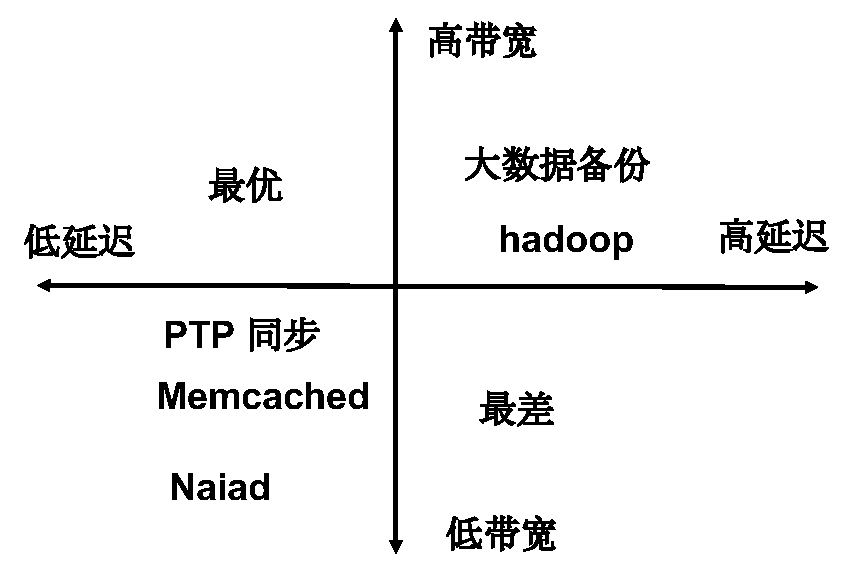
\includegraphics [width=0.9\columnwidth] {figures/others/require.pdf}
\caption{数据中心应用的需求}
\label{relatedwork-require-fig}
\end{center}
\end{figure}


数据中心并存了很多应用,这些应用对带宽和延迟的需求不同,使用TCP策略,带宽服从公平分配的原则。
然而,不同的应用对延迟和带宽需求不同,使用TCP,不能满足所有应用对带宽和延迟的需求。
图\ref{relatedwork-require-fig}显示的是数据中心应用对带宽和延迟的需求,横轴表示的是延迟,纵轴表示的是带宽,
在图\ref{relatedwork-require-fig}坐标系中,从左到右,延迟越来越大,从下到上越来越大。
我们可以看到,对于Hadoop和数据备份,需要高带宽,对延迟需求不大。
对于PTP等应用,对带宽要求不高,但是需要低延迟。
使用TCP协议,对这些应用同等看待,难以满足应用的不同需求,因此,亟需新的方法,考虑应用的不同需求,
智能的分配网络资源,满足应用对网络资源的不同需求。



\section{数据中心网络应用传输方案}
日益使用的数据中心网络尽管有能给应用提供高带宽和低延迟的链路,
 但仍然面临频繁的网络拥塞\cite{Incast08, Incast09}。
传统的TCP协议,难以满足不同的应用对带宽和延迟的需求,针对TCP在数据中心性能不足的问题,业界提出了一系列的方法来弥补。
根据方法优化的粒度,可以分成流级别传输优化方案和任务级别传输优化方案。

\subsection{流级别传输优化方案}
流级别的调度方法,主要侧重提高截止期限前传输完成流的比例,以及优化流的平均完成时间。
从方法上看,流级别的传输优化方法主要可以分成两类,第一种是通过改进传输协议TCP等,调整滑动窗口来调整带宽;
第二种是进行传输调度,采用集中控制的方法,计算流在未来的一个时间段内的传输速率,使的流按照计算出的传输速率进行传输。
本小节,我们从流的传输方法上对流传输进行总结和归类。

\subsubsection{改进TCP的方案} 
在DCN中的许多改进TCP的传输方案中,DCTCP\cite{DCTCP}
提出在交换机的瞬时队列长度超过某个阈值K时,对数据包进行标记,
随后,接收端对被标记的数据包的ACK进行标记,发送端通过统计ACK被标记的比例来计算拥塞程度,
并根据拥塞程度($\alpha$)来调整滑动窗口。
根据拥塞水平$\alpha$,出现拥塞时,滑动窗口变化为w = w$\times$(1 -$\alpha$/ 2)。
通过设置适当的阈值,DCTCP可以使的交换机的队列处于低水平上。
大量的实验表明,DCTCP有效地为短流提供低延迟服务。
然而DCTCP不是根据截止期限进行带宽调整的,
因此对于截止期限敏感的OLDI(Online-Data-Intensive),MapReduce等应用(如网络查询和广告),
DCTCP的调整效果会很差 \cite{D2TCP}。

 D$^2$TCP改进了DCTCP,能更加智能的调整发送端的拥塞窗口。
 它定义了一个期限迫近因子d = T/D,其中T是不采用期限感知的方法,
 传输完成所需要的时间,D是剩余时间。
 出现拥塞时,根据网络拥塞程度$\alpha$和期限迫近因子d的拥塞窗口的调整方法:
$w=w \times (1-\alpha^{d}/2)$。
D$^2$TCP不但具有DCTCP保持排队长度稳定并且队列短的优良特性,
 而且可以使得期限更近的数据流获得更多的带宽。
 D$^2$TCP可以与TCP共存,并且易于在数据中心部署。
 
L$^2$DCT \cite{L2DCT} 尝试减小流完成时间,和D$^2$TCP类似,当出现拥塞时,
L$^2$DCT也使用伽玛校正函数进行滑动窗口调整($cwnd = cwnd*(1-\alpha^{w_c})$)。
L$^2$DCT 近似实现短流优先策略,小的数据流有更高的优先级,因此流平均完成时间变小。
和 D$^2$TCP,DCTCP一样,L$^2$DCT也需要借助网络中ECN的标记。
L$^2$DCT只能够优化流完成时间,而无法优化显式设置期限的数据流。
 
  
TIMELY\cite{mittal2015timely}是基于RTT判断拥塞的协议,
当RTT增大时,TIMELY认为网络中发生了拥塞,发送速率需要降低。
当RTT减小时,TIMELY认为网络拥塞程度轻,可以增大发送速率。
通过RTT进行拥塞判断,TIMELY可以使的交换机队列处于低水平上,从而有效的降低传输延迟。
但是,基于RTT的方法在数据中心存在以下两个问题:首先,数据中心网络中的RTT时间太短,无法准确测量;
而使用RDMA这些新型技术的成本太高。
此外,它不能和基于丢包的策略共存,
因此在实际当中部署存在难度。

ICTCP\cite{ICTCP}通过分析TCP带宽,RTT,和TCP接收窗口(receive window)的关系,
动态的调整TCP接收端的接收窗口(receive window)大小,从而把网络中出现Incast的影响尽量降低。
但是,数据中心RTT的波动大,难以进行测量;
其次,ICTCP侧重于优化网络中的Incast问题,
无法对背景流进行传输优化。

\subsubsection{流调度方案}
 
D$^{3}$ \cite{D3}在集中控制器上计算交换机上所需的带宽,
并把计算的带宽反馈给交换机,使交换机按照计算出的速率发送。
虽然D$^{3}$是第一个已知的基于截止期限进行带宽调整的传输协议,
但是其对数据流优先级调度采用贪心和先到先得的策略,
因此在某些情况下,期限远的数据流会比期限近的数据流优先调度 \cite{D3}。
另一方面,D$^{3}$ 需要修改交换机硬件,因此在实际中部署难度大。

PDQ \cite{PDQ}在端上使用抢占式流量调度来分配带宽。
与D$^{3}$不同,PDQ以分布式方式工作,
其抢占式调度可以处理D$^{3}$无法处理的场景。
PDQ可以使用不同的调度策略,如最早截止期限(Earliest Deadline First,简称EDF)或最短作业优先(Shortest Job First,简称SJF)。
然而,SJF是单一链路上的流平均完成时间最小化的最佳解决方案。
对于复杂链路来说,它并不是最优的。
PDQ使用流平均完成时间被用作评估指标,
PDQ还要求修改交换机的硬件,不能与传统的TCP共存。
 
 PIAS\cite{bai2015information}借助于交换机当中存在的队列, 
 实现了 MLFQ(Multiple Level Feedback Queue )机制。
 在这种机制中,流的优先级开始最高,随着数据发送,
 流的优先级开始降低,PIAS近似实现了短流优先的策略,
 从而间接的优化了流平均完成时间。
 然而PIAS只是优化流平均完成时间,并没有考虑网络拥塞情形,
 当网络拥塞时,并不能满足紧急应用的数据流对带宽的需求。
 
 
QJUMP\cite{grosvenor2015queues}给每个应用分配一个优先级,
对高优先级的应用在发送端进行限速,而一旦数据包进入网络中,
高优先级的数据包可以排在交换机的前列,低优先级的数据包排在交换机队列的后面。
从而实现了高优先级的数据包有较低的延迟,而低优先级的数据包,有更高的网络带宽。
QJUMP在高带宽和低延迟找到了一个平衡,
但是,在实际应用中,应该合理的给应用分配优先级,
如果优先级分配不合理,会导致应用性能降低。
 
 
在FastPass \cite{perry2015fastpass}中,发送端何时发送数据包,
以及发送数据包的路径由中央处理器的计算结果决定。
FastPass借助数据包发送时间算法和数据包发送路径算法来决定数据数据包发送时间和发送路径。
通过这两个算法,FastPass能够在不改变硬件的前提下,
使交换机队列浅,从而降低排队延迟。
FastPass可以有效的降低网络中交换机队列长度,
但是FastPass是集中式控制的方法,集中式控制的方法在数据中心中会增加传输延迟。
此外,如果控制器发生故障,会导致系统崩溃。

pFabric \cite{pFabric}根据流剩余数据量大小进行调度,
pFabric \cite{pFabric}提出的分布式算法近似于最短作业优先(Shortest Job First,简称SJF)策略,
并且被证明在优化流平均完成时间问题上是近似最优策略。
与PDQ相比,pFabric将流量调度与速率控制分离开来,实现起来更加简单,并且可以与类似TCP的方案共存。
pFabric需要单独的交换机,这导致pFabric在网络中难以部署。
 
 
DeTail\cite{DeTail},侧重于跨层技术,
包括流的优先级调度和高效的负载平衡策略,
以减少长流的完成时间的。
尽管能有效的减少网络传输延迟,但是DeTail需要使用新的网络协议,
因此在实际难以大规模使用。


Karuna \cite{chen2016scheduling} 是调度混合流(有期限的流和没有期限的流混合)场景下的解决方案。
Karuna主张,对于有期限的流,要在截止期限之前完成,对于没有截止期限的流,平均流完成时间影响最小。
Karuna \cite{chen2016scheduling} 可以减少流失时间的流量百分比,并减少流的平均完成时间。 
Karuna必须在交换和终端节点上进行改变。
这使得Karuna在实践中部署难度很大。

PASE\cite{PASE}声明的协议(DCTCP,PDQ,pFabric等)不是竞争关系,它们是互补的。
PASE不改变网络中的器件,在减少流完成时间方面性能要比pFabric复杂。
 
\subsection{任务级别传输优化方案}
流级别的传输优化方案,能够优化单条流的完成时间,
或者尽量保证流在截止期限之前完成。
但是,单纯的流级别传输并不能满足应用的需求。
比如web 搜索(分区-聚合模型),数据备份,MapReduce,
分布式存储等应用是包含很多并行的数据流。
对多阶段的应用,只有当上一阶段传输完毕后,下一阶段才能开始传输,
因此,为了应用能够取得更好的性能,需要从流传输任务的级别进行优化。

Orchestra\cite{Chowdhury2011Managing}发现任务传输时间占据了任务总处理时间的33$\%$\cite{Chowdhury2011Managing}。
因此,Orchestra首先提出调度应该侧重优化任务阶段整体传输,而不只是优化某条数据流。
Orchestra使用一个全局的控制器来对所有传输信息进行同步,这个全局控制器存储了所有源和目的节点信息。
对于广播的传输网络传输结构,Orchestra采用Cornet协议,更加合理的利用网络拓扑进行传输优化。
对于shuffle的传输,Orchestra采用权重shuffle调度进行带宽分配。
Orchestra从总体上优化了任务传输,尤其对广播和MapReduce的shuffle阶段性能提升显著。

Barrat\cite{dogar2014decentralized}提出在调度应用的数据传输时,
应该在任务的级别进行,而不是在流级别进行。
Barrat对任务的调度整体采用FIFO模式,对于数据量大的任务,
随着传输进行,降低任务优先级,从而保证大任务不会阻塞链路,影响小任务的传输。
Barrat是一个分布式的任务级别调度系统,
通过对任务的整体调度,Barrat能够有效的减小任务平均完成时间,同时减少任务最长的传输延迟,
进而提升应用的传输性能。


Varys\cite{chowdhury2014efficient}提出对于存在数据并行的应用,
应该以coflow\cite{chowdhury2012coflow}为调度单元,而仅仅在流级别进行优化是不够的。
Varys提出对应用的优化的目标是最小化平均流组(coflow)完成时间。
为了达到这个目标,Varys采用集中式调度策略,首先计算流组的优先级,然后计算每条数据流的带宽。
对于流组优先级,Varys采用最小瓶颈优先(Smallest-Effective-Bottleneck-First,简称SEBF)启发式算法来决定。
最小瓶颈优先策略策略是把一个流组(coflow)中传输最慢的流的完成时间当做流组的预估完成时间,
然后根据预估传输时间进行排序,使得预估完成时间小的流组获得高优先级。
对于数据流的带宽的控制,使用最小带宽期望(Minimum-Allocation-for-Desired-Duration,简称MADD)算法。
使用集中控制的方法,借助以上两个策略,Varys优化了平均流组完成时间(Coflow Completion Time,简称CCT),从而提高了应用的性能。

Varys需要预先得知很多流组(coflow)的信息,
事实上,在数据中心中,很多应用的流组(coflow)中流的大小信息是很难预先得知的,尤其在hadoop多阶段计算中,
中间shuffle会传输大量数据,数据流的大小很难被预先得知。
基于此,Aalo\cite{chowdhury2015efficient}提出,在调度coflow时,应假设预先不知流组(coflow)中流的大小进行调度。
Aalo实现了最短流组优先策略 ,
根据已经发送数据量的大小,把流组(coflow) 分配到不同的优先级队列中。
相同的优先级队列中的流组(coflow)采取FIFO调度机制。
Aalo近似实现最短流组(coflow)优先的策略,整体上调度了流组(coflow),从而优化了流组(coflow)的传输效率。

事实上,无论Aalo还是Varys,都需要提前分别出应用的流组(coflow),这需要对应用进行改动。
而修正比如Hadoop和Spark等应用的API需要考虑兼容性和进行Java-byte级别的改动,这导致修改的复杂度较高。
CODA\cite{zhang2016coda}首先尝试不改变应用,来自动的区分和调度应用流组(coflow)。
同时使用late binding等措施来尽量减少流组(coflow)区分的错误等。
通过对应用的流组(coflow)进行有效的区分和带宽的调度,
CODA从整体上对coflow实现了调度,从而,有效的降低了应用流组(coflow)的传输时间,优化了应用传输延迟。


和Varys,以及Aalo等相同,D-CAS\cite{luo2016towards}将数据网络假设成非阻塞交换机,
认为传输冲突只发生在交换机的入端口以及出端口,中间路径并没有拥塞发生。
D-CAS提出coflow最小化平均传输完成时间调度问题和开放商店中任务平均工作完成时间问题的优化等价。
为了优化coflow传输延迟,D-CAS改进了开放商店中的任务平均完成时间的2-近似算法\cite{roemer2006note},
并将2-近似调度算法引入到流组(coflow)的调度中,然后改进2-近似调度策略,从而得到流组(coflow)的在线调度算法。
D-CAS采用分布式的方法实现,可以有效的减小流组(coflow)的传输时间。



RAPIER\cite{zhao2015rapier}打破了数据中心非阻塞体系结构,
认为在传输中,拥塞随时发生,不只发生在第一跳和最后一跳。
传输时不应只考虑调度问题,为每条数据流分配合理的路径是很重要的问题。
基于此,RAPIER把流组(coflow)的路径选择和流组(coflow)的调度放在一起考虑,
通过求解非整数优化问题,把每条数据流发送速率的大小和发送路径都计算出来。
RAPIER可以减少平均CCT在50$\%$以上,并且易于在真实环境中部署。
和Varys相同,RAPIER需要预先得知coflow中每条数据流大小等信息。


Task-aware TCP\cite{liu2017task}认为传统的TCP-based方法只考虑了单一流的情形,
而没有考虑流之间的关系,这会影响流之间的传输,导致传输效率低。
Task-aware TCP主张,在一个task中,速率过快的数据流应该把带宽让给速率慢的数据流。
Task-aware TCP\cite{liu2017task}改进了DCTCP方法,借助于ECN标记,区分出传输过快和传输过慢的数据流,
把传输过快的数据流带宽给传输过慢的数据流一些,
从而使的任务的平均传输时间减少,进而优化了任务的传输延迟。




Qiu在\cite{qiu2015minimizing}从理论角度考虑有权重的流组(coflow)的调度,
假设已经知道coflow到达时间,每条流的信息进行调度。
Qiu同时强调调度流组(coflow)时,应该也同时考虑权重,而不应该把所有流组(coflow)同等看待。
使用近似算法,Qiu提出的策略,可以达到$\frac{67}{3}$的近似比。
使用随机性策略,算法的近似度可以达到$9+16\frac{\sqrt{2}}{3}$。
Qiu在\cite{qiu2015minimizing}通过求解方程组对流组(coflow)进行调度求解,此方法有较高的复杂度,
在实际中难以部署。


\subsection{数据中心传输方案存在的问题}
相比于传统的TCP,当前数据中心传输方案能够有效的提高数据中心传输效率,
提高应用对网络等资源的使用情况,
然而,尽管数据中心网络技术在不断发展,
但是,随着应用业务的不断发展,数据中心网络始终难以满足应用的各种需求,
因此,需要更加合理的网络资源调度来满足应用对网络资源的需求。
当前数据中心网络依然存在以下的问题:

\textbf{(1)未考虑网络拥塞程度和应用传输期限关系}

D$^3$首先提出,在进行传输时,
应该给数据流分配足够多带宽,让数据流满足期限。
D$^3$改动交换机,并在交换机上计算出数据流传输满足期限的最小带宽,
从而数据流能够获得足够多的带宽,从而在期限之前完成。
D$^2$TCP根据网络的拥塞情形和数据流期限调整数发送窗口,
通过拥塞窗口间接的影响数据流传输的带宽,进而实现不同需求的数据流达到各自传输的目的。
这两种方法都同时考虑了数据流传输的期限和网络拥塞状况。
然而,无论哪种方法,都没有考虑网络拥塞程度,期限的二维关系。
事实上,尽管D$^2$TCP考虑了数据流的传输应该同时考虑网络期限,
但是当网络拥塞程度严重时,D$^2$TCP不再是基于期限调整的拥塞控制策略。
因此,如何合理的根据网络拥塞情形,期限调整数据流传输是亟需解决的问题。


\textbf{(2)无法同时满足延迟敏感流和带宽敏感流的需求}

数据中心中同时存在对延迟敏感的短流和对带宽敏感的背景流。
当前的数据中心的传输方案,无论是D$^2$TCP,
D$^3$还是L$^2$DCT都是解决单一数据流的需求,
即或者满足延迟敏感流的需求,或者满足带宽敏感流的需求,
比如D$^2$TCP,D$^3$侧重优化有显式期限的流,
L$^2$DCT优化的是流平均完成时间,
并不能同时满足这两种数据流的需求。

\textbf{(3)任务级别调度只考虑网络拥塞并没有考虑任务的重要性}

尽管Varys,Aalo等策略在调度数据中心资源时,
是在任务级别进行的,
但是这些策略只是考虑网络的拥塞状况,
目标是优化应用的传输完成时间。
然而,应用有不同的语意,只考虑应用的传输是不够的,应该同时兼顾应用的重要性。
比如,进行计算的hadoop和视频传输业务共享数据中心资源,
进行计算的hadoop的业务的优先级比进行视频传输业务的优先级高,
使用传统的传输策略,会认为这两个应用数据流的优先级相同,
这样常会导致进行计算的Hadoop业务的数据流得到的带宽不足,
造成Hadoop的完成时间过长,从而影响应用的整体性能并且造成网络资源利用率偏低。

基于以上的几个问题,本文从流级别和任务级别对传输策略进行优化和改进,
使的流的带宽能够根据网络拥塞和流的期限进行动态调整,
同时对混合场景下的流传输进行优化,
使有期限的数据流和对带宽敏感的数据流都能满足需求。
最后从任务级别对传输进行了优化。

\section{本章小结}
本章中,我们综述了数据中心应用传输方案的相关工作。
我们从常见应用的通信模型和数据流量等方面对数据中心传输进行了概述。
然后,我们总结了流级别和任务级别的数据中心传输方案进行。
最后,我们总结了数据中心传输方案存在的问题。















\chapter{基于ECN标记的流传输模型}
\label{chap:model}

\section{本章引言}
本章中,我们介绍基于ECN标记的流模型。
首先,我们对基于ECN标记的流模型的场景进行介绍。
然后,我们介绍基于ECN标记的流模型,
最后,我们根据基于ECN标记的流模型实例化DCTCP,
得到DCTCP流模型,作为ECN标记的流模型的一个实例。

\section{场景描述}
传统TCP通过调整拥塞窗口来进行速率的控制,
当网络不拥塞时,拥塞窗口每个RTT增加1 MSS,
当网络中出现拥塞时,TCP拥塞窗口减半。
通过对TCP滑动窗口的调整,TCP实现了对发送速率的控制。

\begin{figure}[H] 
  \centering
  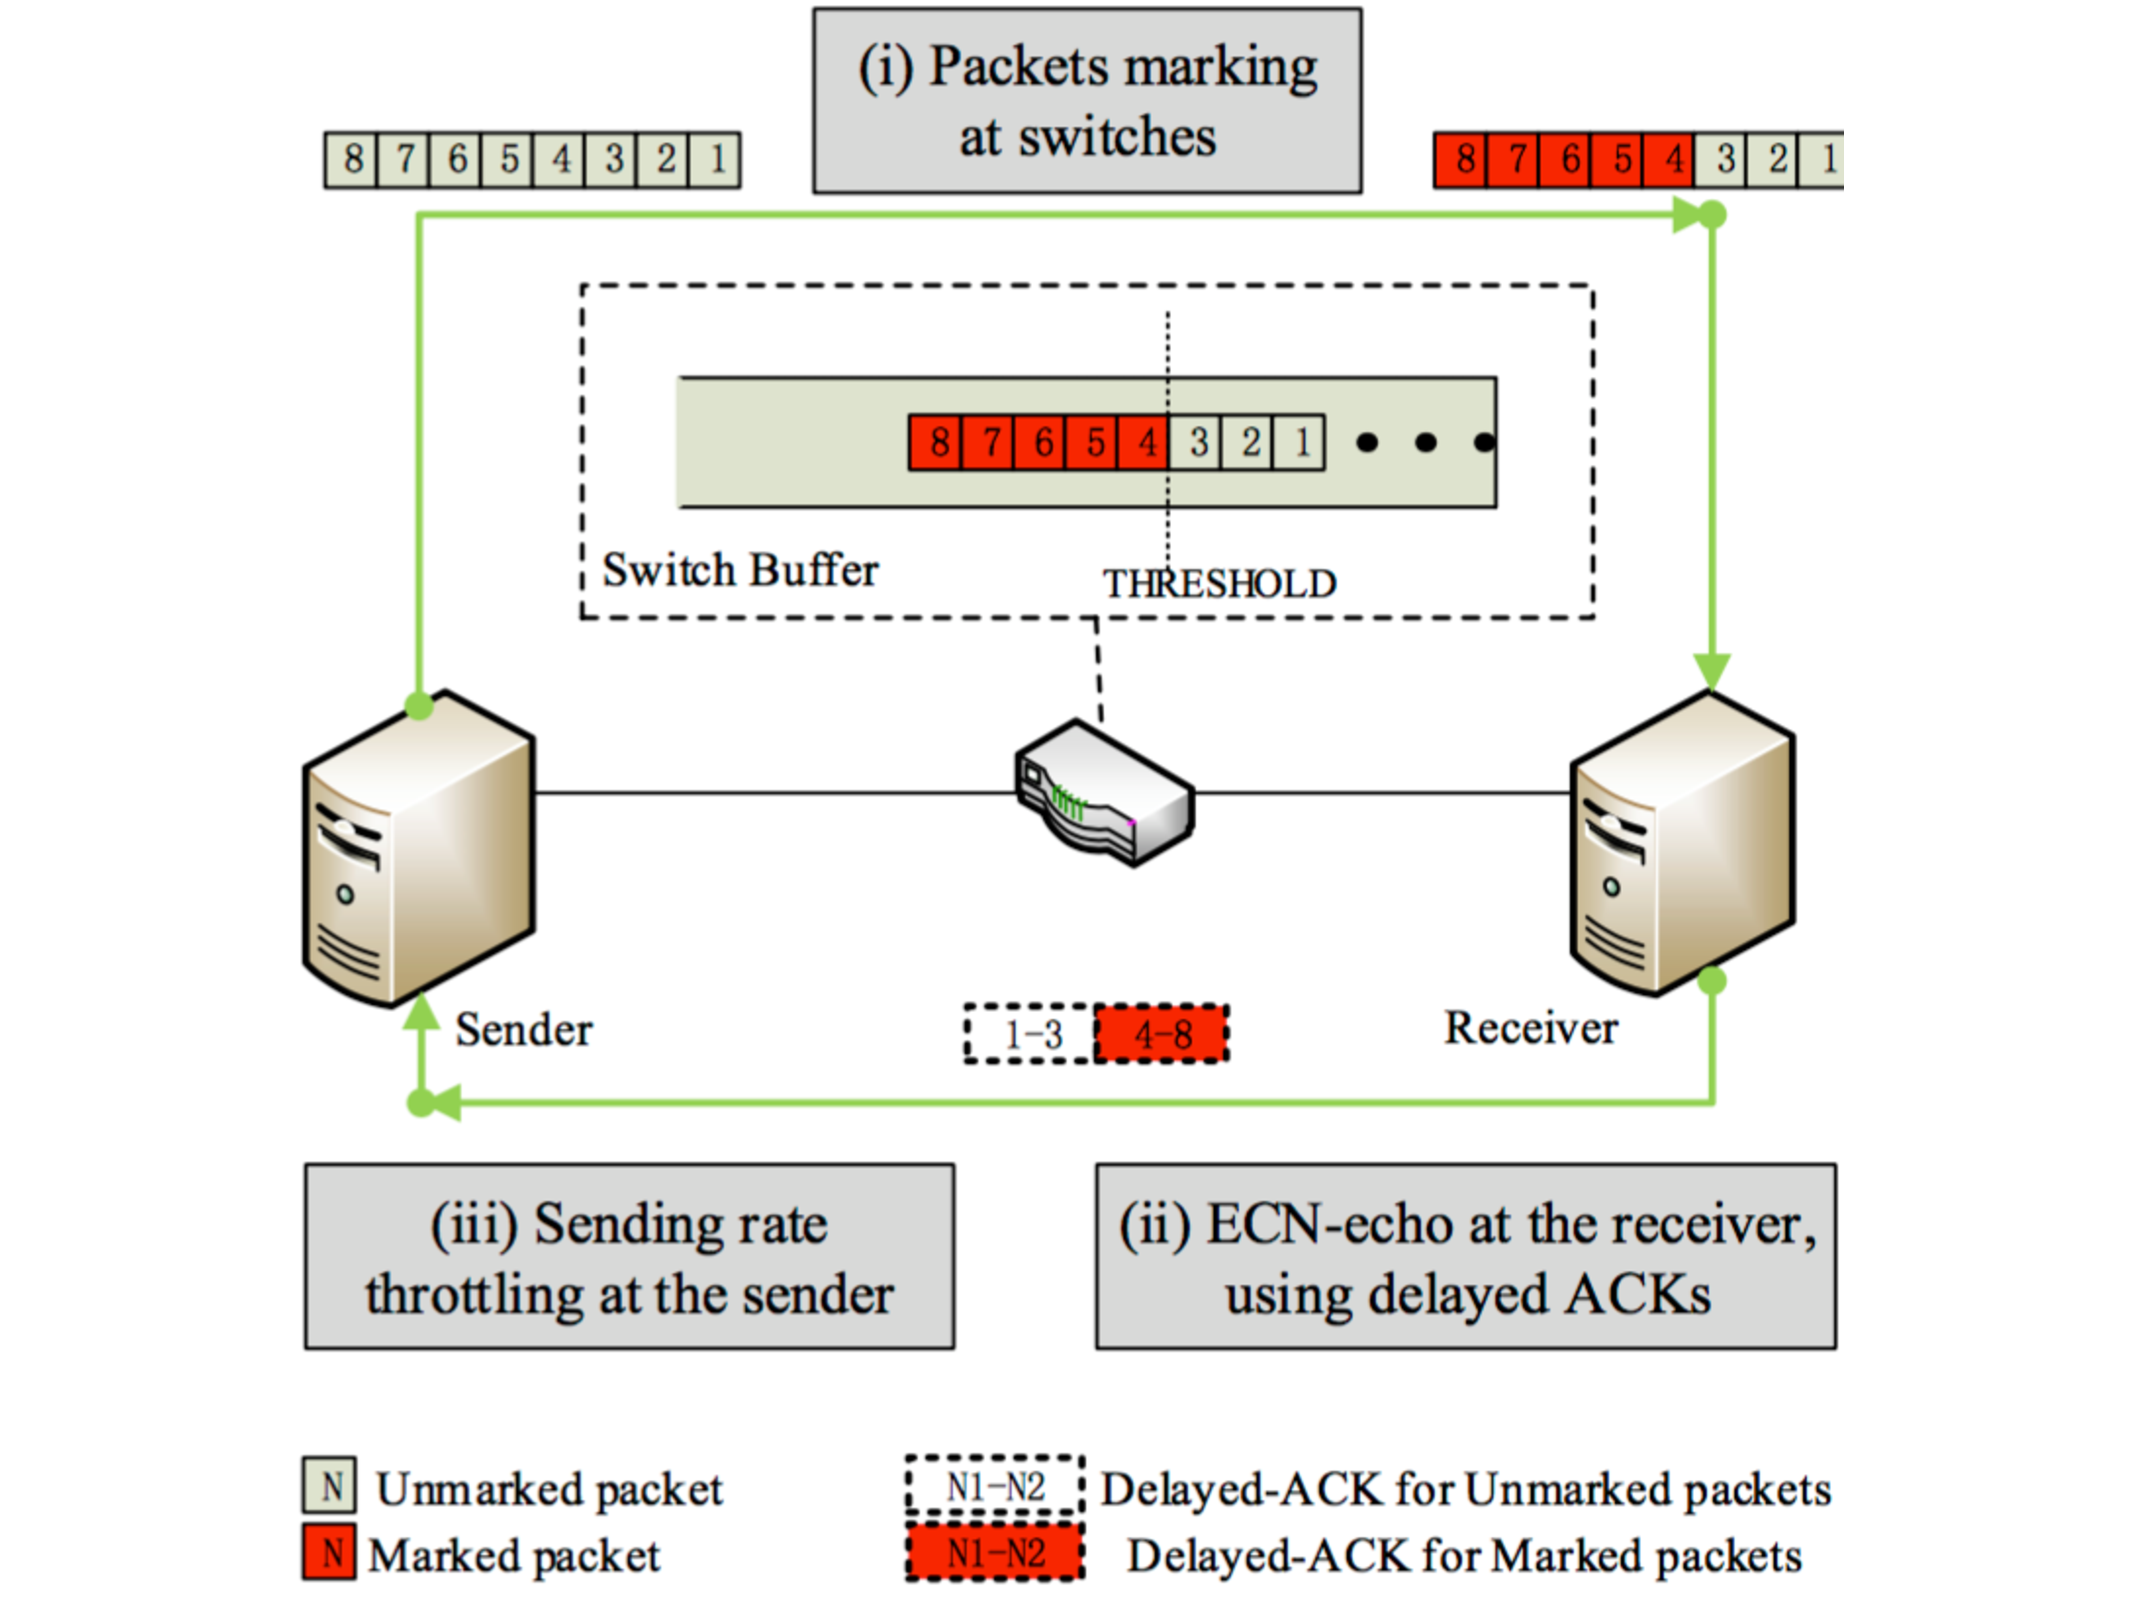
\includegraphics[width=0.9\columnwidth]{figures/others/model-process.pdf}
  \caption{基于ECN标记的数据中心速率控制过程,交换机上设置阈值,当排队队列超过阈值后,进行标记,发送端根据被标记的数据包比例,动态调整发送窗口}
  \label{model-process-fig}
\end{figure}

基于ECN标记的拥塞控制速率机制过程如图\ref{model-process-fig}所示:首先,发送端发送数据包给交换机,在交换机设置一个阈值,
当交换机队列长度超过阈值后,超过交换机设置队列设置阈值的数据包会被标记CE(和TCP不同,TCP会丢包)。
当接受端收到数据包后,检查数据包是否被标记CE,
如果发送的数据包被标记CE,那么给发送端回复的ACK中标记ECN。
发送端检查收到的ACK中被标记ECN的ACK的比例,以此来计算网络的拥塞程度$\alpha$,根据拥塞程度进行拥塞窗口的计算。

当网络中没有拥塞时(此RTT时间内没有被标记的数据包),滑动窗口每个RTT增加$(1-f_1(\alpha))$,
当网络中有拥塞时(此RTT时间内中有被标记的数据包),滑动窗口减小$f_2(\alpha)$倍。
其中$f_1(\alpha)$和$f_2(\alpha)$是关于拥塞程度$\alpha$的函数。
(\ref{Model-CA-eq})是基于ECN标记的拥塞避免阶段窗口变化的公式。

\begin{equation}
w=
\begin{cases}
w+(1-f_1(\alpha)) &\text{没有拥塞}\\
w \times (1-f_2(\alpha)) &\text{出现拥塞}
\end{cases}
\label{Model-CA-eq}
\end{equation}




\section{ECN标记流模型}\label{cha:model:introduction}




\begin{figure}[H] 
  \centering
  \includegraphics[width=0.9\columnwidth]{figures/others/senders.eps}
  \caption{N个发送端发送数据给1个接收端}
  \label{model-senders-fig}
\end{figure}

如图\ref{model-senders-fig}所示,假设N个发送端连接1个交换机,1个接收端连接在交换机上。
N个发送端使用公式(\ref{Model-CA-eq})进行拥塞控制窗口的计算。
交换机支持ECN标记,当交换机队列满足ECN标记条件时,发送到交换机的数据包会进行数据包标记。

\subsection{模型描述}

公式(\ref{fluid-model_window})$\sim$(\ref{fluid-model-q})是基于ECN标记的描述模型,
其中(\ref{fluid-model_window})表示的是窗口变化过程,其中,第一部分$\frac{1-f_1(\alpha)}{R(t)}$描述的是窗口增加的过程,
其中每个RTT窗口增加$1-f_1(\alpha)$。
$\frac{w_i(t)f_2(\alpha)}{R(t)}p(t-R^*)$描述的是窗口减小的过程,当发生拥塞时,窗口减小$\frac{w_i(t)f_2(\alpha)}{R(t)}$。
其中$p(t-R^*)$表示的是否出现ECN标记,当$p(t-R^*)=1$时,表示ACK中有ECN标记,当$p(t-R^*)=0$时,表示ACK中没有ECN标记,
此时网络中没有拥塞。

公式(\ref{fluid-model_queue})表示的是交换机队列变化,
$ \sum_{i=1}^N{\frac{w_i(t)}{R(t)}}$表示的是发送到交换机的数据包,
假设交换机的转发速率是C pkt/s,那么,交换机的队列长度是$\sum_{i=1}^N{\frac{w_i(t)}{R(t)}}-C \label{fluid-model_queue}$。

公式(\ref{fluid-model-q})是交换机是否进行标记,当交换机队列满足一定条件$F({q}(t))==1$时,
进行标记的函数$\widehat{p}(t)=1$,否则,$\widehat{p}(t)=0$。
 \begin{align}
&\frac{dw_i}{dt}=\frac{1-f_1(\alpha)}{R(t)}-\frac{w_i(t)f_2(\alpha)}{R(t)}p(t-R^*)  \label{fluid-model_window} \\
&\frac{dq}{dt}= \sum_{i=1}^N{\frac{w_i(t)}{R(t)}}-C \label{fluid-model_queue}  \\
&\widehat{p}(t)=1_{F({q}(t))==1}  \label{fluid-model-q}
\end{align}




\subsection{模型实例}

本章节,我们使用DCTCP\cite{DCTCP}来验证模型,DCTCP协议在交换机上设置阈值K,
当交换机的队列超过K时,数据包被打标记,同时在发送端滑动平均拥塞程度$\alpha$:

\begin{equation}
\alpha=(1-g)\times \alpha+g\times F
\label{Model-alpha-eq}
\end{equation}

其中,g为滑动平均因子,F为当前RTT中被标记ECN的数据包,
当前滑动平均拥塞程度$\alpha$为上一个RTT的打标记的ECN比例F和当前计算的平均拥塞程度的比例值。
在DCTCP中,$f_1(\alpha)=0$,$f_2(\alpha)=\frac{\alpha}{2}$,
将$f_1(\alpha)$和$f_2(\alpha)$带入(\ref{Model-CA-eq})得到拥塞控制函数:

\begin{equation}
w=
\begin{cases}
w+1 &\text{没有拥塞}\\
w \times (1-\frac{\alpha}{2}) &\text{出现拥塞}
\end{cases}
\label{Model-CA-DCTCP-eq}
\end{equation}
同时把$f_1(\alpha)$和$f_2(\alpha)$带入(\ref{fluid-model_window})$\sim$(\ref{fluid-model-q}),
并且改动(\ref{Model-alpha-eq}),得到:

 \begin{align}
&\frac{dw_i}{dt}=\frac{1}{R(t)}-\frac{w_i(t)\alpha}{2R(t)}p(t-R^*)  \label{DCTCP-fluid-model_window} \\
&\frac{dq}{dt}= \sum_{i=1}^N{\frac{w_i(t)}{R(t)}}-C \label{DCTCP-fluid-model_queue}  \\
&\frac{d\alpha_i}{dt}=\frac{g}{R(t)}(p(t-R^*)-\alpha_i(t)) \label{DCTCP-model_alpha} \\
&\widehat{p}(t)=1_{q(t))>K}  \label{DCTCP-fluid-model-q}
\end{align}

其中,(\ref{DCTCP-fluid-model_window})是描述的是DCTCP的窗口,
(\ref{DCTCP-fluid-model_queue})描述的是队列长度,当没有出现拥塞时,拥塞窗口每个RTT增加1,当出现拥塞时,滑动拥塞窗口减小$\frac{\alpha}{2}$。
特别的,(\ref{DCTCP-model_alpha})是描述的拥塞程度$\alpha$,
(\ref{DCTCP-fluid-model-q})中被标记的条件是队列长度大于K。
设置g=1/16,C=10Gbps,N=2,K=64,
图\ref{DCTCP-analysis-fig}是对DCTCP实例化的模型进行的验证并且使用ns-2和模型结果进行对比的结果。

\begin{figure}[h]
\centering
\subcaptionbox{$\alpha$}
 {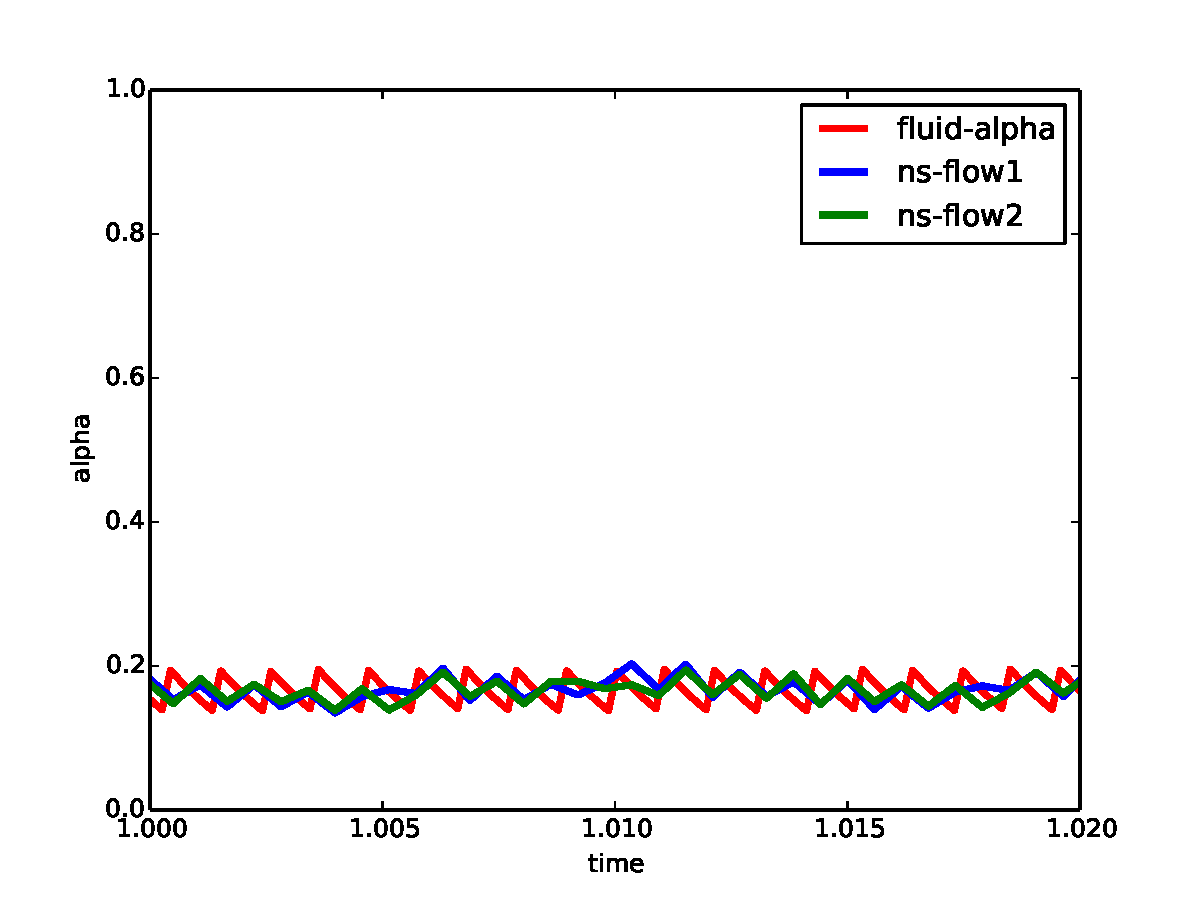
\includegraphics[width=0.32\columnwidth]{figures/others/DCTCP/alpha.pdf}}
\subcaptionbox{队列长度}
{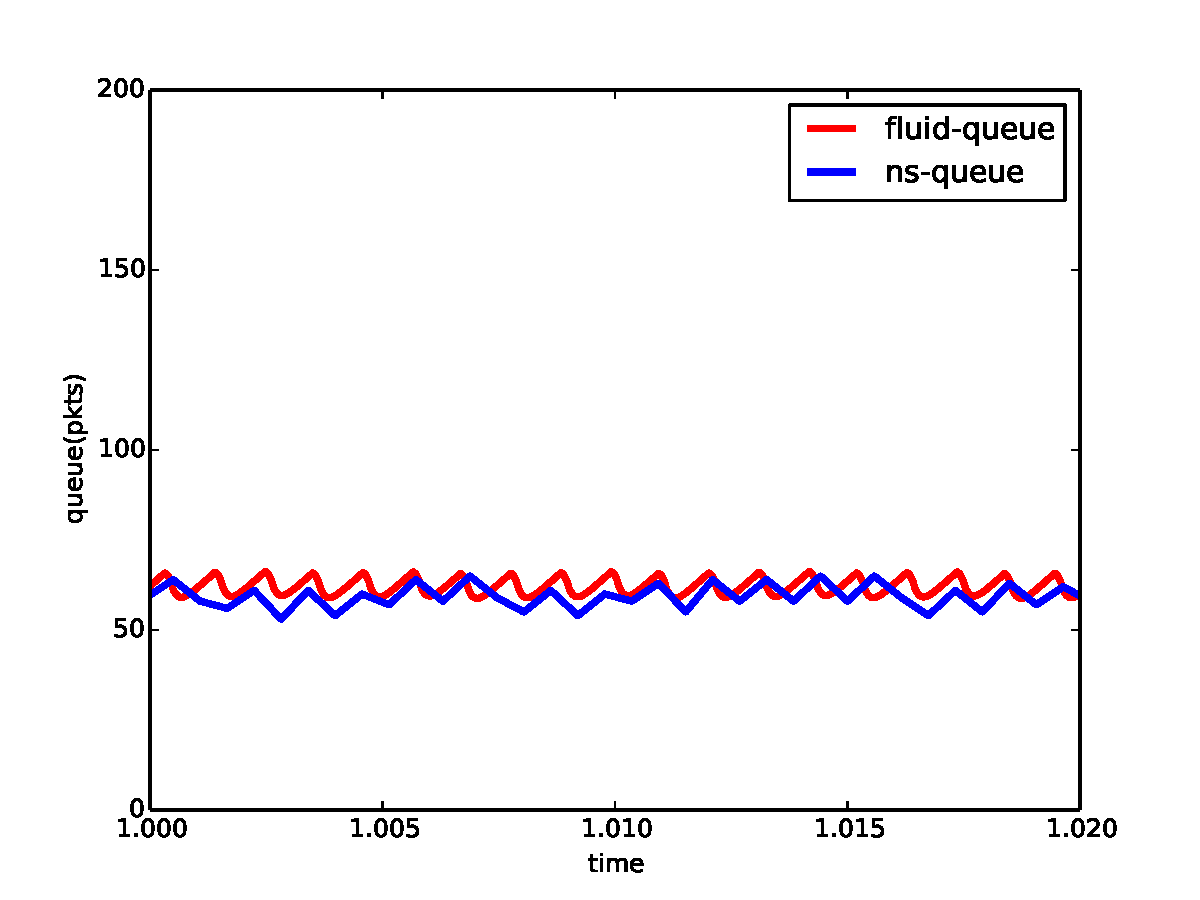
\includegraphics[width=0.32\columnwidth]{figures/others/DCTCP/queue.pdf}}
\subcaptionbox{窗口大小}
{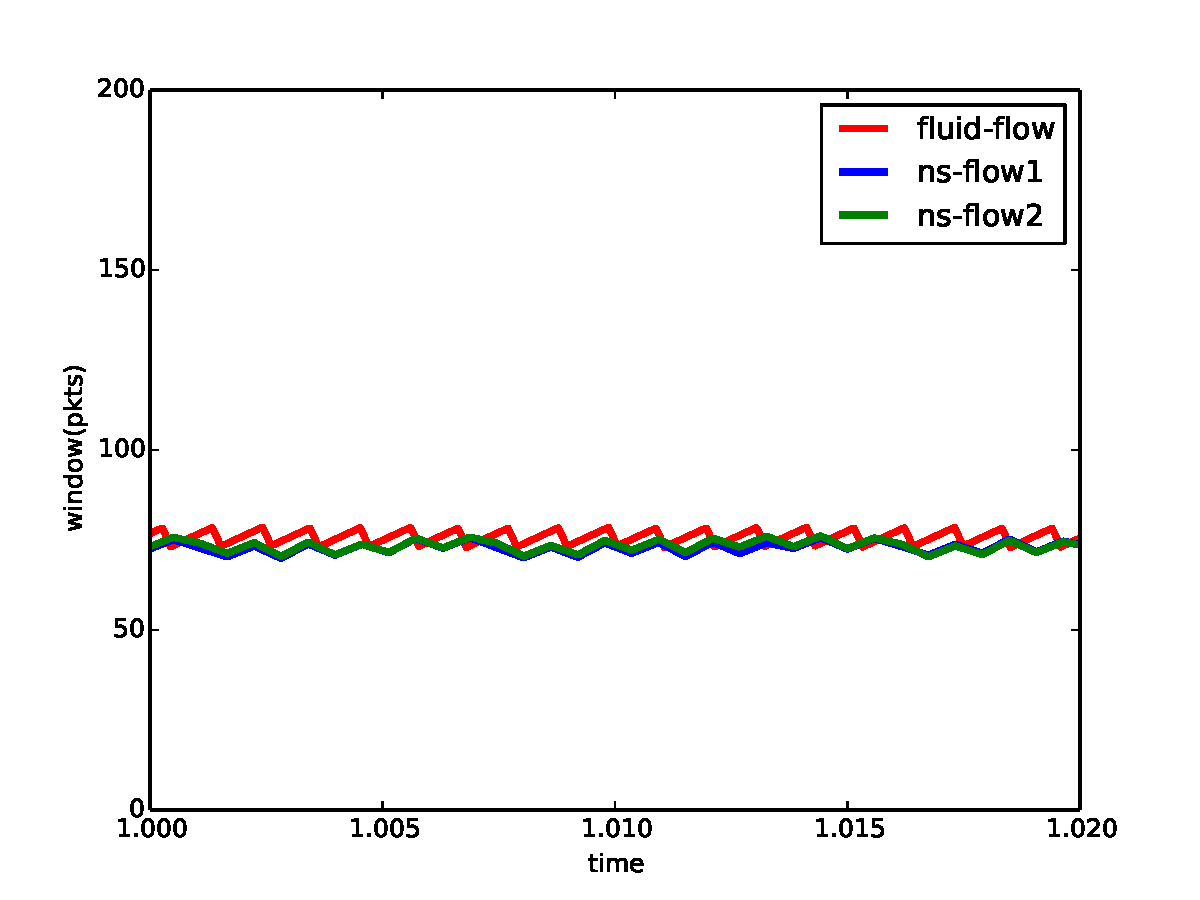
\includegraphics[width=0.32\columnwidth]{figures/others/DCTCP/window.pdf}}
\caption{DCTCP中标记ECN流模型推算结果和ns-2下结果对比}
\label{DCTCP-analysis-fig}
\end{figure}

图\ref{DCTCP-analysis-fig}(a)描述的是拥塞程度$\alpha$,
图\ref{DCTCP-analysis-fig}(b)描述的是队列长度,
图\ref{DCTCP-analysis-fig}(c)描述的是拥塞窗口,
我们可以发现,通过模型进行描述推倒的结果和仿真的结果基本相同。
因此,使用模型可以有效的描述基于ECN标记的传输协议。

\section{本章小结}
本章中,我们介绍了基于ECN标记的流模型。
我们介绍了基于ECN标记的流模型的场景和基于ECN标记的流模型。
最后,我们根据基于ECN标记的流模型实例化DCTCP,
得到DCTCP流模型,作为ECN标记的流模型的一个实例。
\chapter{基于负载自适应原则的传输优化方案}
\label{chapter:LPD}
现在很多在线应用部署在数据中心,因此数据中心网络的性能和底层技术吸引了越来越多的研究者的兴趣。
为了达到更好的网络性能,
近期的研究从不同角度优化数据中心网络流量传输和调度,并且设计各种路由和传输方案。
特别是对于必须及时为用户服务的应用,有的必须在截止时间之前完成,否则会影响用户体验。
传统的传输策略TCP并不能满足数据中心应用的需求。
针对此,最近业界出现了一系列的考虑流传输期限的网络流量控制策略。
尽管这些方案能够在一定程度上提升数据中心应用传输的性能,然而,当网络拥塞程度严重时,这些策略基本失效,不再根据期限进行带宽区分。
本章主张在设计数据流传输方案时,
应该遵循一个简单的原则:
拥有不同截止期限(deadline)的数据流在带宽分配和占用上应该被区分开,
并且网络负载越重,流带宽越应被区分。

根据此原则,本章并提出了简单的拥塞控制算法-正比负载差分策略
(Load Proportional Differentiation,简称LPD)作为其应用。
同时本章在不同的拓扑和负载情况下评估LPD。
本章发现与D$^2$TCP(最先进的基于期限拥塞控制滑动窗口策略)相比,
LPD错过最后期限的流的比例减少25$\%$以上。
与Karuna相比,LPD平均有5$\%$的性能损失。
但是在拥塞严重的情况下,LPD性能比Karuna高5$\%$ $\sim$10$\%$。
事实上 “越拥塞,越区分”是一个通用的原则,也可以用于其他目标的优化,
本章考虑优化流平均完成时间。
与基于窗口的协议L$^2$DCT相比,LPD可以将流平均完成时间减少30$\%$。
和最先进的流平均完成时间优化策略pFabric相比,LPD只有20$\%$的性能损失。 


\section{概述}
\label{sec_LPD:Introduction}
目前,越来越多的服务和应用,如网络搜索和社交网络被托管在数据中心\cite{chowdhury2014efficient,chen2016scheduling,zhang2016fdrc,chowdhury2012coflow,chowdhury2015efficient}。
由于数据中心网络的性能,特别是数据传输时延,吞吐量等直接影响到用户获得的服务的质量,
因此需要设计新的网络协议,充分利用数据中心提供的网络资源。
在数据中心网络(DCNs)中,短流需要低延迟,
长流需要高吞吐量\cite{DCTCP,chen2016scheduling}。
为了满足这些要求,最近的研究提出了各种针对数据中心流量进行控制的策略。


特别是,在数据中心普遍部署了一类称为在线数据密集型(Online Data Intensive,简称OLDI)\cite{OLDI,D2TCP} 的重要应用。
这类应用需要为用户提供实时服务。
实时服务对延迟要求很高,即使增加1毫秒的延迟也会对企业利润产生影响\cite{Latency}。
实时应用通常需要查询和收集来自节点的反馈结果。
为了不影响用户体验,反馈结果需要在截止期限之前传输完成。
如果某些应用的计算结果尚未计算完毕开始传输,应用会向用户发送不完整的反馈结果,这会影响最终反馈结果,从而影响用户体验。
错过期限的流越少,服务质量越高,用户的体验越好。
像TCP或DCTCP这类没有考虑期限的传输方案会导致错过期限的流数目较多,
而当前很多数据中心流量控制算法\cite{D3, D2TCP}或流量调度算法\cite{PDQ}中明确地考虑了截止期限。



本章重点研究了数据中心基于期限的流量控制算法。
本章首先分析不同业务负载情况下D$^2$TCP性能,
当网络负载很高的情形下,D$^2$TCP退化为DCTCP,并且不再是基于期限的拥塞控制策略。
基于此,本章认为当网络负载较重时,应该为截止期限较近的流分配更多带宽。
本章提出一个简单的基于期限的速率控制方案:
拥有不同期限的流在带宽分配上应该被区分,
并且网络负载越重,期限不同流的带宽差异程度越大。


为证明此原则的有效性,本文设计了一个简单的基于期限的拥塞速率控制算法-
正比负载差分策略(Load Proportional Differentiation,简称 LPD)作为其应用。 
LPD的基本思想是:使用截止期限来调节拥塞窗口时,网络负载应作为调整因子引入其中,
数据流的区分调整程度与网络负载成正比。
本文使用典型的数据中心拓扑和各种业务负载场景来评估LPD的性能,
并将其与一些最新的数据中心流量控制算法(例如DCTCP \cite{DCTCP} ,D$^2$TCP \cite{D2TCP}和L$^2$DCT \cite{L2DCT},Karuna\cite{chen2016scheduling})进行对比。
实验结果显示,LPD性能总是能超过这些策略,LPD能使更多流在截止期限之前完成。
与D$^2$TCP相比,LPD可以将错过最后期限的流的比例减少25$\%$以上。
和最先进的基于期限的拥塞控制方法Karuna相比,LPD的性能平均差5$\%$。
但对于一些较为拥挤的场景,由于LPD采用“越拥塞,越区分”的设计原则,
在拥塞程度严重的时候,LPD的性能比Karuna好10$\%$。
此外,“越拥塞,越区分”是一般性的原则,
它可以用来优化其他目标,诸如减少流平均完成时间。
本文修改LPD以使其适合于优化流平均完成时间,
然后将其性能与最先进的基于窗口的优化流平均完成时间的协议L$^2$DCT进行比较,
发现LPD比L$^2$DCT在流平均完成时间方面缩短30$\%$。
即使与最先进的优化流平均完成时间的方法pFabric \cite{pFabric}相比,LPD的性能差20$\%$。
本文随后在ns2 \cite{ns2,LPD-sim-code}上和Linux kernel 3.2.61 \cite{LPD-code}中实现并且评估LPD。

本章的主要工作如下:

(1)测试并发现当前DCNs中基于期限的拥塞控制策略在网络重度拥塞严重的情形下失效。

(2)提出了“越拥塞,越区分”的原则来设计DCNs中的基于截止期限流量控制机制,并在数学上确定了遵循这一原则的方案的充分和必要条件。
 
(3)提出LPD算法作为“越拥塞,越区分”原则的一个应用,并建立基于ECN的数据流传输模型来分析它的性能。
 
(4)在ns-2和linux内核3.2.61中实现LPD,并且把LPD的性能和当前最流行的基于期限的速率控制策略进行对比。
 
 
为了保证本章的实验可以重复,本文同时对LPD代码开源。
LPD的模拟代码可以在\inlinecite{LPD-sim-code}下载,
LPD的Linux内核源代码可以在\inlinecite{LPD-code}中找到。
本文还根据“越拥塞,越区分”的原则设计了其他的拥塞控制策略,
并且说明此策略是具有普遍性的。
 
 \section{研究动机}
 \label{sec_LPD:Motivation} 
D$^2$TCP给不同的数据流分配不同大小的带宽,
使期限近的流获得更多带宽。
本文认为这是一个重要的尝试,
但是在拥塞控制中仅仅考虑期限是不够的,网络拥塞也应被考虑。
 
 
 \begin{table}[h]
\centering
\caption{D$^2$TCP和DCTCP仿真结果对比}\label{flowtable}
\renewcommand{\arraystretch}{1.5}
\begin{tabular}{|c|c|c|c|c|c|} \hline
\setlength{\tabcolsep}{10pt}
 & D$^2$TCP &  DCTCP \\ \hline
flow 1  (8 MB, 200 ms)   &1.53 MB &2.07 MB \\ \hline
flow 2  (16 MB, 400 ms)   &1.79 MB &2.14 MB \\ \hline
flow 3  (32 MB, 600 ms)   &3.64 MB &4.08 MB \\ \hline
flow 4  (40 MB, 800 ms)   &0 MB    &0 MB \\ \hline
\end{tabular}
\end{table}


\begin{figure}[h]
\setlength{\abovecaptionskip}{0pt} 
\setlength{\belowcaptionskip}{1pt} 
  \centering%
  \subcaptionbox{流的带宽\label{LPD_Motivation:subfig1}} %标题的长度,超过则会换行,如下一个小图。
    {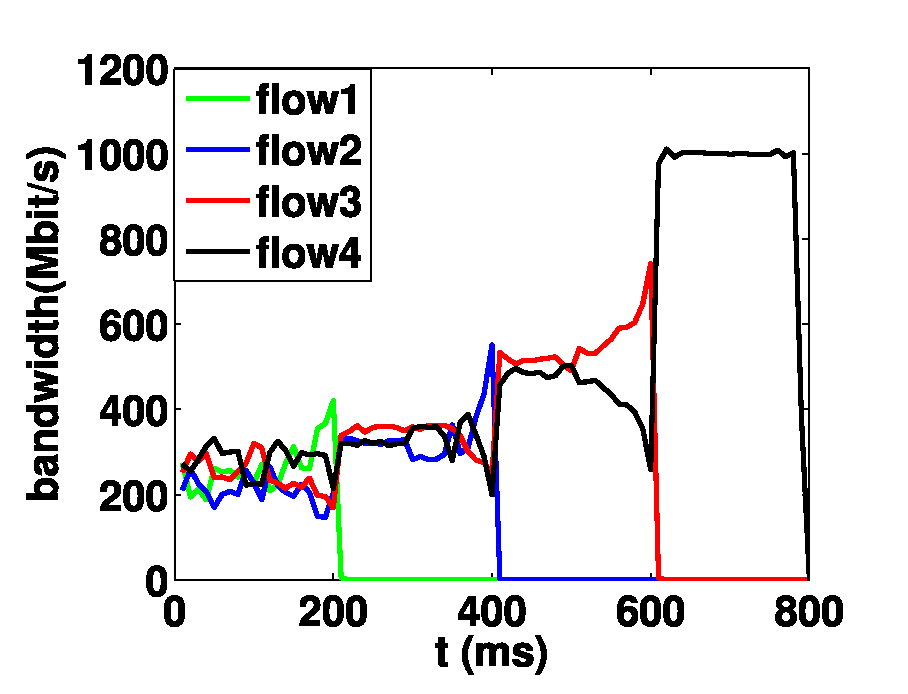
\includegraphics[width=0.5\columnwidth]{figures/LPD/bandwidth.eps}}%
  \subcaptionbox{拥塞窗口\label{LPD_Motivation:subfig2}}
      {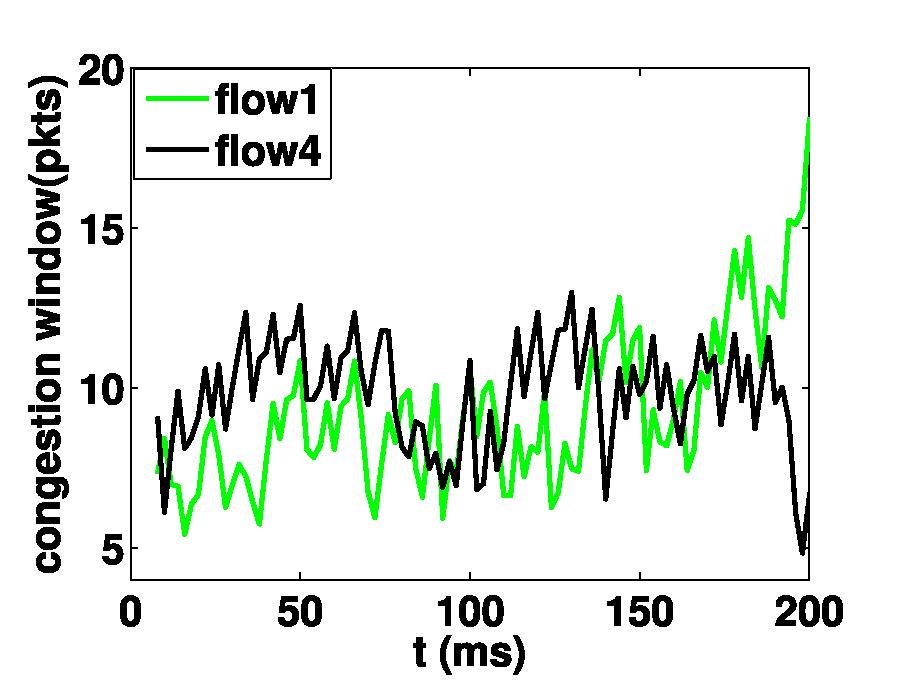
\includegraphics[width=0.5\columnwidth]{figures/LPD/cwnd.eps}}
  \subcaptionbox{flow$_1$和flow$_4$的期限因子\label{LPD_Motivation:subfig3}}%标题的长度,超过则会换行,如下一个小图。
    {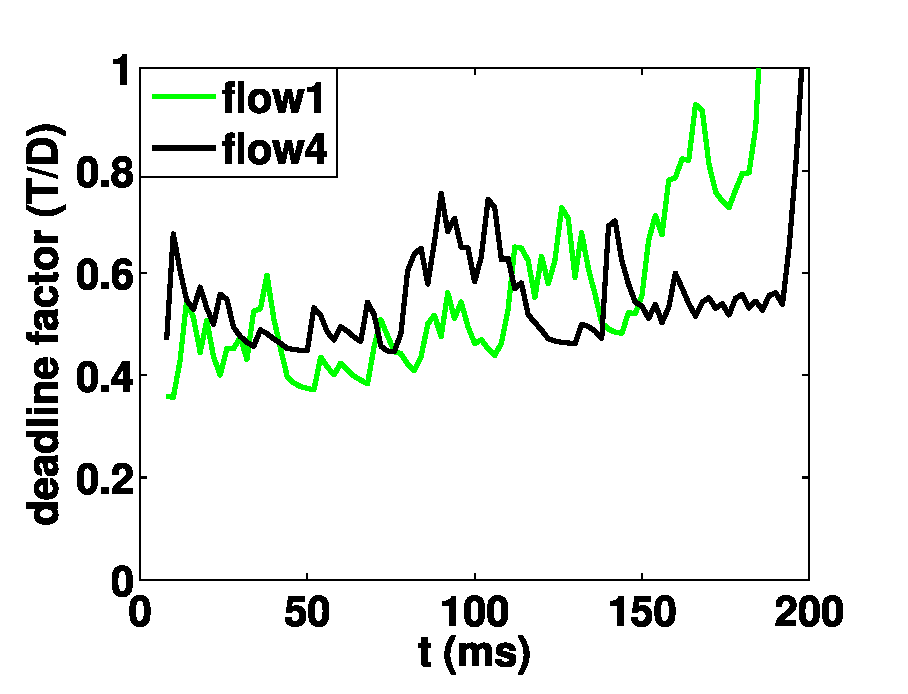
\includegraphics[width=0.5\columnwidth]{figures/LPD/deadlinefactor.eps}}%
  %\hspace{7em}%
  \subcaptionbox{flow$_1$和flow$_4$的拥塞因子\label{LPD_Motivation:subfig4}}
      {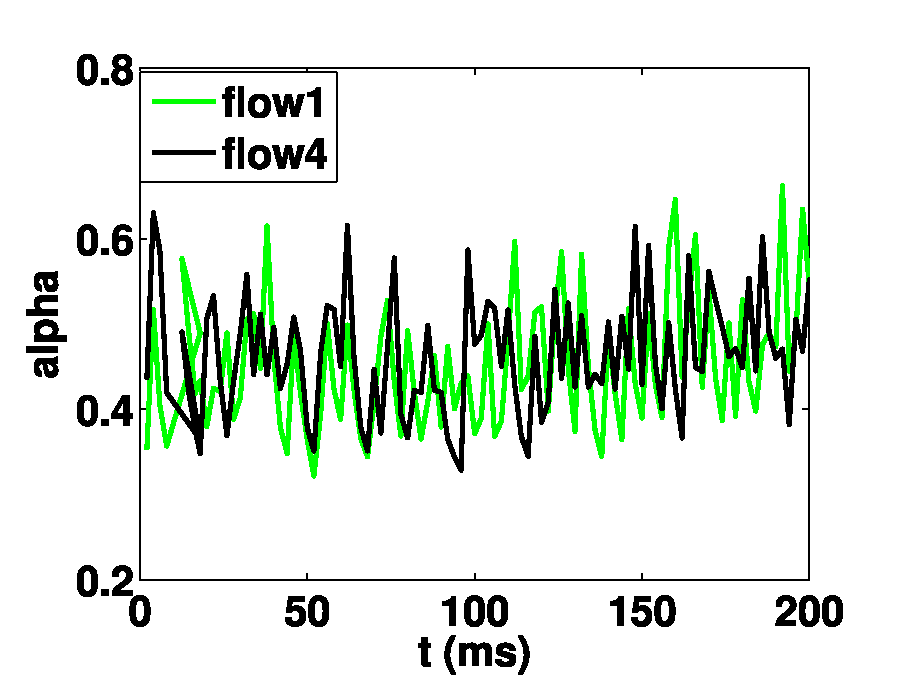
\includegraphics[width=0.5\columnwidth]{figures/LPD/alpha.eps}}
  \caption{D$^2$TCP的性能:4条并发流}
  \label{LPD_Motivation}
\end{figure}

\begin{figure}[h]
\centering
\subcaptionbox{$p=\alpha^d$\label{LPD_Gamma:subfig1}}
 {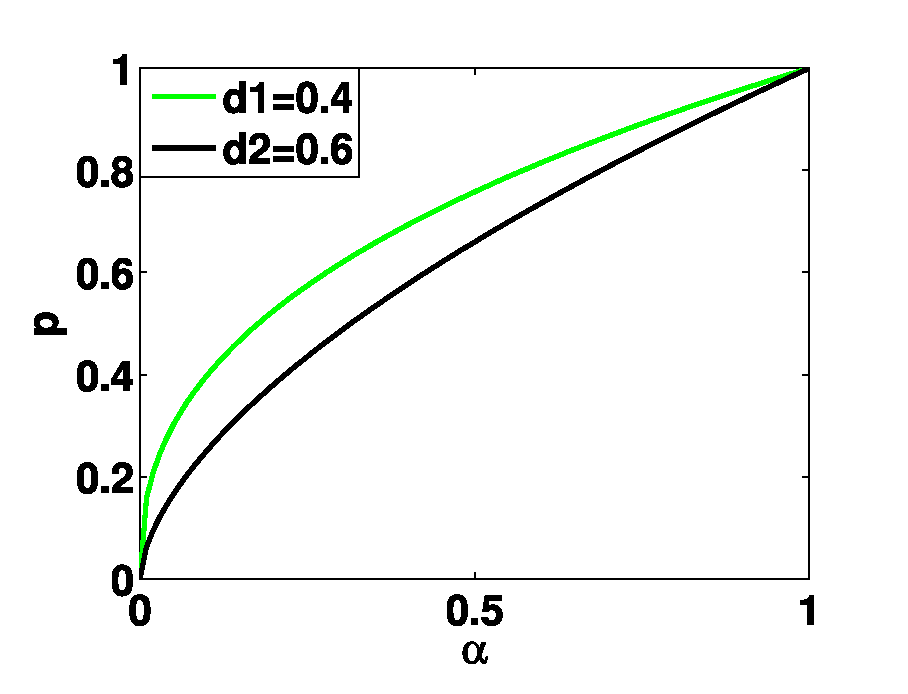
\includegraphics[width=0.45\columnwidth]{figures/LPD/gamma.eps}}
\subcaptionbox{$pd=p(\alpha, d_{1})-p(\alpha, d_{2})$\label{LPD_Gamma:subfig2}}
{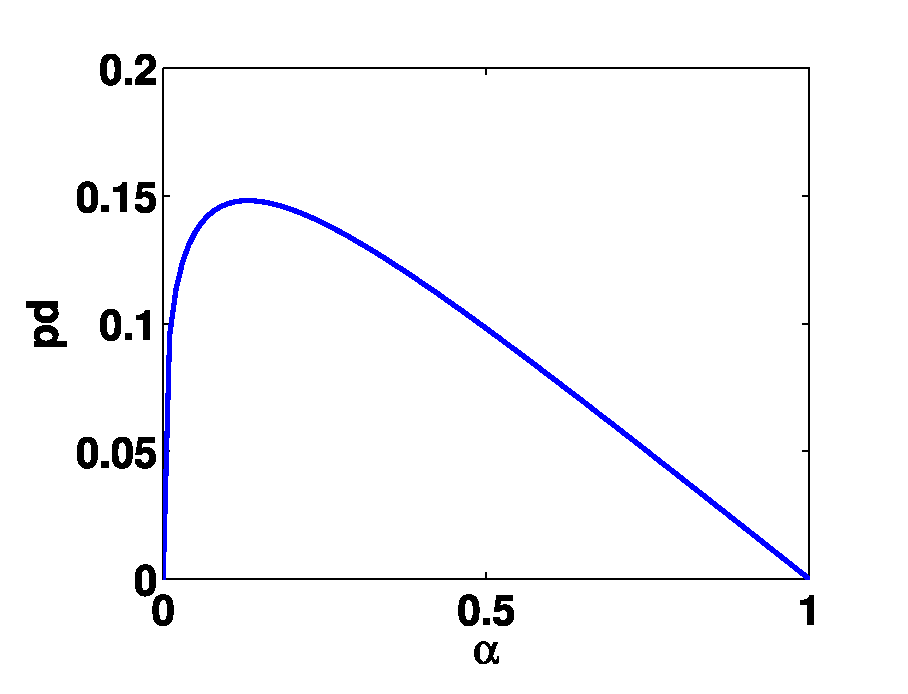
\includegraphics[width=0.45\columnwidth]{figures/LPD/PD.eps}}
\caption{D$^2$TCP 使用伽马校正函数来减小拥塞窗口}
\label{penalty-fig}
\end{figure}


为了验证D$^2$TCP存在的问题,使用ns-2进行如下仿真:四条流通过瓶颈带宽为1Gbps的链路,
流同时启动,大小分别为8,16,32和40 MB,截止期限分别为200,400,600和800 ms,设置RTT为100 us。
事实上,如果使用TCP,则可以使得所有流在800ms之前完成。
使用DCTCP和D$^2$TCP的流传输结果如表\ref{flowtable}所示。
表\ref{flowtable}中第2列和第3列的每个数字表示DCTCP和D$^2$TCP在流截止期限到达时未发送的数据量
(传输完成后,数据流会被强制停止)。
从表\ref{flowtable}可以看到,尽管D$^2$TCP在流截止期限之前传输的数据比DCTCP多,但不能有效地减少错失期限流的数目。
无论DCTCP还是D$^2$TCP,只有flow$_4$在截止期限之前完成。
根据实验结果显示,当拥塞程度严重时,D$^2$TCP的性能和DCTCP的性能基本相同。 
图\ref{LPD_Motivation}显示了传输的更多细节,
图\ref{LPD_Motivation}(a)描绘了flow$_1$和flow$_4$的带宽:大部分时间内流之间带宽差别很小。
图\ref{LPD_Motivation}(b)是flow$_1$和flow$_4$在最初200ms期间的拥塞窗口大小:
除了快接近最后的10ms时,flow$_1$的窗口会比flow$_4$大很多之外,大部分时间,flow$_1$和flow$_4$的窗口差别不大。
图\ref{LPD_Motivation}(c)是flow$_1$和flow$_4$的期限迫近因子:,二者的期限迫近因子相差很大,特别是在100 ms到200 ms的时间内。
图\ref{LPD_Motivation}(d)是表示flow$_1$和flow$_4$对拥塞程度的一种评估:二者估算的拥塞程度基本相同。
可以发现,尽管flow$_1$和flow$_4$有相同的拥塞程度,不同的截止期限,但是二者的期限因子基本相同。
 
 
 \section{“越拥塞,越区分”的设计原则}
 \label{sec_LPD:MORE_LOAD}
D$^2$TCP试图将截止期限引入到拥塞窗口计算中,
进而期限不同的流计算得到不同的期限因子。
本章首先发现和分析D$^2$TCP在重度拥塞时失效的原因。
然后提出截止期限的速率控制策略的设计原则,并对之进行数学描述。
最后本章提出正比负载差分策略LPD,并对之进行简单分析。

\subsection{D$^2$TCP分析}
\label{sec_LPD:gamma}
D$^2$TCP的核心思想是在惩罚函数中使用伽马校正函数p($\alpha$,d)=$\alpha^d$,其中0 <$\alpha$<1。
图 \ref{penalty-fig}(a)显示的是d = 0.4和d = 0.6时伽马校正函数的曲线。
可以发现,当$\alpha$增加时,较正函数(p)增加,即网络越拥塞,滑动窗口减小越多,流带宽减小越多。
然而,如果考虑惩罚函数的差异,即相同拥塞情形下的不同期限的流较正函数:
例如$pd(\alpha, d_{1}, d_{2})=p(\alpha, d_{1})-p(\alpha,d_{2})=\alpha^{d_{1}}-\alpha^{d_{2}}$,
其中$d_{1}$ <$d_{2}$。
发现pd首先随$\alpha$的增加而增加,
在$\alpha$经过某一点(图\ref{penalty-fig}(b)中0.2左右)之后减小。
例如,pd(0.4,0.4,0.6)= 0.116,
pd(0.6,0.4,0.6)= 0.079,
而pd(0.9,0.4,0.6)= 0.019。
因而,网络拥塞程度较重的环境中,D$^2$TCP对期限不同数据流的调整能力基本失效,
不再是基于拥塞程度进行速率控制的方法。
 
 
解释在研究动机的实验中,D$^2$TCP在网络重度拥塞时失效的原因:
在150ms到160ms的时间间隔,$\alpha$从0.4增加到0.6,flow$_1$和flow$_4$的紧急因子分别是$d_1$ = 0.6和$d_4$ = 0.4,
因而flow$_1$比flow$_4$更紧急。
然而,pd(0.6,$d_4$,$d_1$)= 0.079,pd(0.4,$d_4$,$d_1$)= 0.116。 
如图\ref{LPD_Motivation}(b)所示,当网络拥塞程度变大时,
flow$_1$的窗口和flow$_4$的拥塞窗口大小基本相同,此时pd(0.9,$d_4$,$d_1$)=0.019,即此时二者计算的期限因子基本相同。
因而,flow$_1$在截止期限之前无法获得足够的带宽,从而无法在截止期限之前完成。
实际中,当网络拥塞程度更严重时,更需要不同截止期限的流应获得不同的带宽,从而流均可在截止期限之前完成。


\subsection{基于截止期限的速率控制策略设计原则}
\label{sec_LPD:principle}

对于OLDI应用,由于查询流并发数目高,网络负载常常很大。
基于此,本文主张在设计基于截止期限的网络拥塞控制策略时应遵循以下原则:

(1)紧急原则(PI):截止期限近流获得的带宽应该高于截止期限远的流获得带宽。

(2)差异原则(PD):当网络负载变大时,截止期限不同的流获得的带宽的差异应该增加。 


PI表示数据流速率应该根据流的截止期限进行区分:考虑两条大小相同的数据流(长度一致),
截止期限近的流应该使用比截止期限远的流获得更多的带宽,
从而流在截止期限之前完成的概率会变大。
PI已经在新的基于TCP的拥塞控制方案(如D$^3$和D$^2$TCP)被采纳。
但是,当前基于TCP的拥塞控制方案,忽略了拥塞和数据流带宽差异之间的关系。


PD表示网络负载越重,流之间带宽差异性应该越大。
与网络负载较轻时相比,网络负载较重时,每条数据流获得的带宽都会减少。
从而,流错失期限的可能性会变大。 
因此,为了尽可能的让数据流在截止期限之前完成,
期限近的流应从期限远的数据流抢夺带宽。
 
因此,截止期限不同的两条流获得带宽的差异性在拥塞程度大的情况下应该更大。
通过此方式,截止期限近的流和截止期限远的流都能在截止时间之前完成。
事实上,当前基于截止期限的拥塞控制策略忽略网络拥塞和不同期限的流带宽差异性之间的关系。
在形式上,假设r($\alpha$,d)表示在网络拥塞情形为$\alpha$(0 <$\alpha$<1),紧急因子为d(d> 0)的情形下流的带宽,$\alpha$越大表示网络越拥塞。定理\ref{theorem-principle}是对PI和PD的数学描述:

\begin{lemma}\label{theorem-principle}
 $r$ 遵守PI和PD的充分必要条件是 $\frac{\partial{r}}{\partial{d}}>0$, 
并且 $\frac{\partial^{2}{r}}{\partial{d}\partial{\alpha}}>=0$ 
(但是不能恒为0)

\end{lemma}


\begin{proof}
引理\ref{theorem-principle}中第一个式子表示PI:r是d的增函数。
说明期限因子越大,惩罚函数也越大,当出现拥塞时,滑动窗口减小的少。
下面证明说明第二个式子表示PD:
定义 $dr(\alpha, d_{1}, d_{2})=r(\alpha, d_{2})-r(\alpha, d_{1})$.
存在:
\begin{eqnarray}\label{eqn-partial}
\frac{\partial{dr(\alpha, d_{1}, d_{2})}}{\partial{\alpha}}
&=&\frac{\partial \left[r(\alpha, d_{2})-r(\alpha, d_{1}) \right]}{\partial{\alpha}} \nonumber \\
&=&\frac{\partial{r(\alpha, d_{2})}}{\partial{\alpha}} - 
\frac{\partial{r(\alpha, d_{1})}}{\partial{\alpha}}
\nonumber \\
&=& \int_{d_{1}}^{d_{2}}\!\!\frac{\partial^{2}{r}}{\partial{\alpha}\partial{d}} \,\,\mathrm{d}d.
\end{eqnarray}

考虑PD的数学意义,PD等价于: 
$dr(\alpha_{2}, d_{1}, d_{2})>dr(\alpha_{1}, d_{1}, d_{2})$
, $\alpha_{1}<\alpha_{2}$ 并且 $d_{1}<d_{2}$ 时成立, 
根据 (\ref{eqn-partial}),
当且仅当
$\frac{\partial{dr(\alpha, d_{1}, d_{2})}}{\partial{\alpha}}>0$
,$d_{1} < d_{2}$成立
, 如果有
$\frac{\partial^{2}{r}}{\partial{\alpha}\partial{d}} \ge 0$ (但是不能恒为0)
\end{proof}

上面提出的原则简单并且有通用型。而在实际部署策略时,如何设置流的截止期限,
以及如何设计由$\alpha$和d作为参数的惩罚函数,可以根据具体的应用来确定。 
在下一小节中,本文将根据这个原则开发一个具体的根据截止期限和网络拥塞函数进行拥塞控制的策略-正比负载差分策略。

\section{正比负载差分策略(LPD)以及分析}
\label{sec_LPD:LPD}

\subsection{正比负载差分策略(LPD)}
作为”越拥塞,越区分”原则的一个应用,可以提出下面基于期限的拥塞控制算法:
\begin{equation}
w=
\begin{cases}
w+(1-f) &\text{没有拥塞}\\
w \times (1-f) &\text{出现拥塞}
\end{cases}
\label{LPD-CA-eq}
\end{equation}


其中f=$\alpha$/d是惩罚函数,
此函数是根据网络负载$\alpha$和紧急因子d进行计算的,因子可以用来区分流的紧急程度。
拥塞程度(即网络拥塞负载因子$\alpha$)的含义和DCTCP以及D$^2$TCP中的相同\cite{DCTCP, D2TCP}。 
由于f与$\alpha$成正比,所以我们称这个算法为正比负载差分策略(Load Proportional Differentiation,简称LPD )。 

定义一个简单的迫近因子d = $t_{max}/t$,
其中t是流开始时间时刻和截止时刻之间的持续时间,
$t_{max}$是t的可调上界,后面会有详细讨论。
对于没有截止期限的流,t可以设置为$t_{max}$。 
t越小,d越大,因此流也越迫切。
基于此,可以得到LPD-t,一个根据网络拥塞和截止期限进行拥塞控制的策略:

\begin{equation}
w=
\begin{cases}
w+(1-\alpha \times \frac{t}{t_{max}}) &\text{没有拥塞;}\\
w \times (1-\alpha \times \frac{t}{t_{max}}) &\text{出现拥塞}
\end{cases}
\label{LPD-t-eq}
\end{equation}


根据(\ref{LPD-t-eq})我们可以看到LPD-t是一个简单策略:
首先计算惩罚函数$f=\alpha \times \frac{t}{t_{max}}$ ,
根据f的值来调控拥塞窗口。
如果网络中没有拥塞,那么拥塞窗口每个RTT增加$(1-f)$,
如果发生拥塞,那么拥塞窗口减小f倍。
 
\subsection{LPD简单分析}
在类似TCP的方案中,通过调整拥塞窗口来间接的调整流的发送速率。
因此,可以通过调整拥塞窗口的大小来调整发送速率。
LPD-t是符合本文提出“越拥塞,越区分”的设计原则的,
引理\ref{theorem-LPD}对此进行了证明。
 
\begin{lemma}\label{theorem-LPD}
LPD 服从 PI 和 PD. 
\end{lemma}
\begin{proof}
$\frac{\partial{(1-f)}}{\partial{d}}
=\frac{\partial{(1-\alpha/d)}}{\partial{d}}
=\frac{\alpha}{d^{2}}>0$, 
并且
$\frac{\partial^{2}{(1-f)}}{\partial{d}\partial{\alpha}}
=\frac{1}{d^{2}}>0$, 
因此LPD-t窗口的限制,满足引理 \ref{theorem-principle}, 
因此LPD-t满足 PI 和 PD。
\end{proof}

从几何角度来看LPD遵循PI和PD这两个原则。 
由于f与$\alpha$成正比,
所以($\alpha$,f)的几何表示是一条穿过原点的直线,窗口变化服从线性规则。
如果两条流有不同的期限因子d,则两条数据流的惩罚函数f之间的差会随着$\alpha$的增大而增大。
引理\ref{theorem-LPD_2}展示在两条流的场景下,LPD-t稳定速率与期限成反比。


\begin{lemma}\label{theorem-LPD_2}
假设LPD-t可以使流收敛在一个稳定的状态,
即拥塞窗口在一个固定的区间内稳定的波动,
此时流有稳定的发送速率,并且计算出的拥塞程度趋于稳定状态。 
如果$t\ll t_{max}$,其中t和$t_{max}$是在(\ref{LPD-t-eq})中LPD-t使用的调整$t_{max}$参数,
则流达到的稳定速率与之对应的期限成反比。
\end{lemma}


\begin{proof}
在稳定状态中,流的拥塞窗口变化规律是固定周期为$N$的锯齿形。 
使用 $W_{min}$ 和 $W_{max}$来代表一个周期内的最小和最大窗口,我们有:

$W_{max}=W_{min}+N \times (1-\alpha \times \frac{t}{t_{max}})$, 
并且 $W_{min}=W_{max} \times (1- \alpha \times \frac{t}{t_{max}})$, 
根据上面,我们有
$W_{max}= N \times (1-\alpha \times \frac{t}{t_{max}})/(\alpha \times \frac{t}{t_{max}})$, 
并且平均窗口大小为: $W_{av}= (1- \alpha \times \frac{t}{2t_{max}}) \times W_{max}$。

对于两条流,$f_{1}$ 和 $f_{2}$。
两条流的持续时间为 $t_{1}$ 和 $t_{2}$, 
假设两条流的最大窗口是$W_{1}$ 和 $W_{2}$, 
流稳定的发送速率为 $r_{1}$ 和 $r_{2}$, 
 两条流的速率比例,$\frac{r_{1}}{r_{2}}$ 可以计算如下:
\begin{eqnarray}
\frac{r_{1}}{r_{2}} &=& \frac{(1-\alpha \times \frac{t_{1}}{2t_{max}}) \times W_{1}}{(1-\alpha \times \frac{t_{2}}{2t_{max}}) \times W_{2}} \nonumber \\
&=& \frac{t_{2}}{t_{1}} \times \frac{2t_{max}-\alpha \times t_{1}}{2t_{max}-\alpha \times t_{2}} \times \frac{t_{max}-\alpha \times t_{1}}{t_{max}-\alpha \times t_{2}} \nonumber
\end{eqnarray}
如果$t \ll t_{max}$, 然后 $r_{1}/r_{2} \approx t_{2}/t_{1}$.
\end{proof}

\begin{figure}[h]
\centering
\subcaptionbox{单条流的带宽}
 {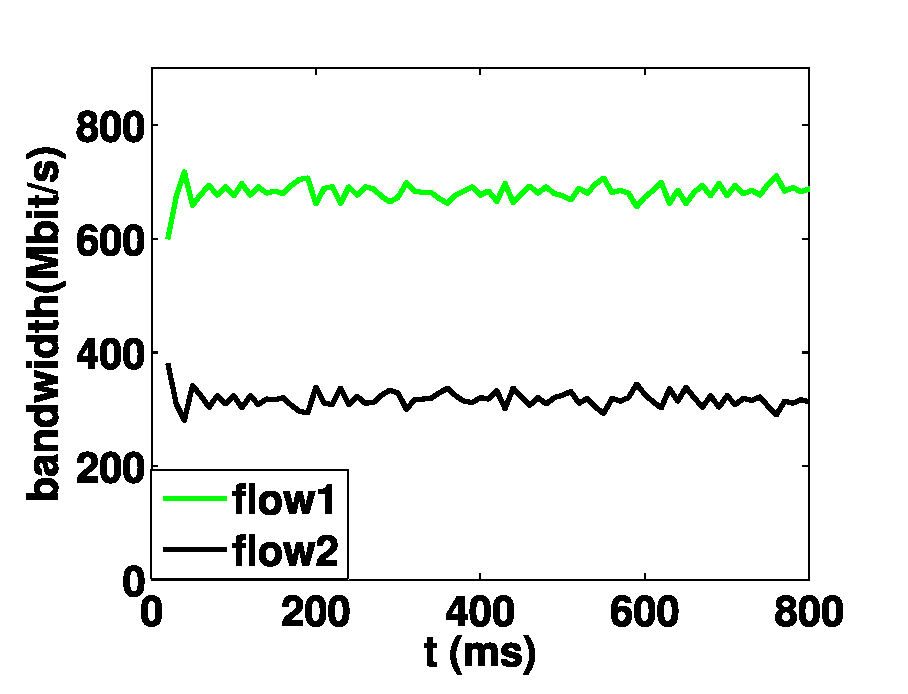
\includegraphics[width=0.45\columnwidth]{figures/LPD/rate2.eps}}
\subcaptionbox{$pd=p(\alpha, d_{1})-p(\alpha, d_{2})$}
{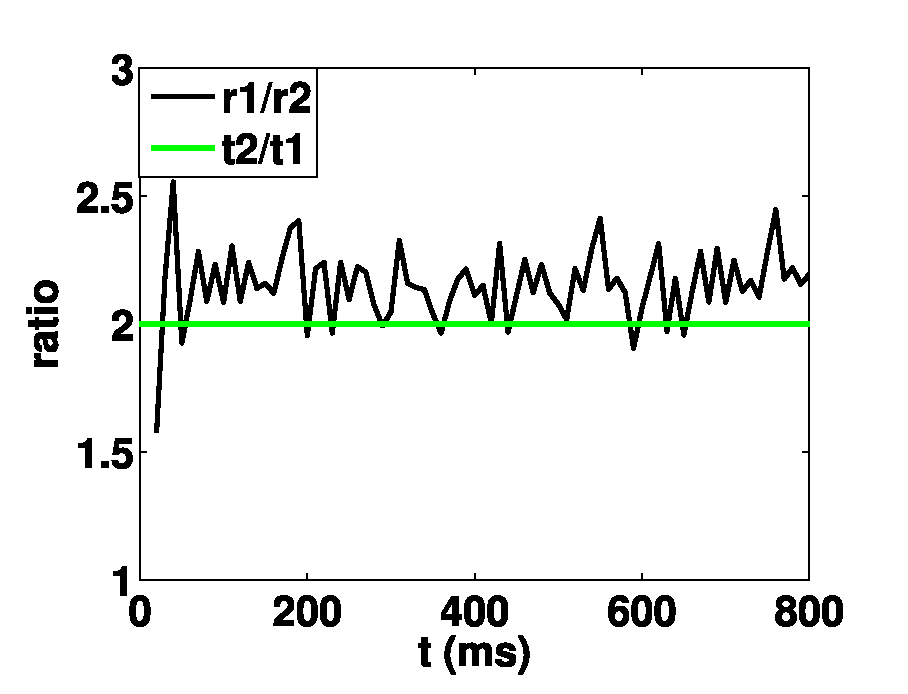
\includegraphics[width=0.45\columnwidth]{figures/LPD/ratio.eps}}
\caption{LPD下的两条流}
\label{rate-analysis-fig}
\end{figure}

尽管LPD-t的稳定性还没有得到证实。
实际上,流截止期限不能比$t_{max}$小太多。
为了验证引理\ref{theorem-LPD_2},进行以下验证: 
启动两条均为100 MB的LPD-t长流,两条流的截止时间为$t_1$ = 5s,$t_2$ = 10s,设置$t_{max}$ = 50s。 
图\ref{rate-analysis-fig}(a)描述了前800 ms流的带宽变化过程,
可以看到,flow$_1$的带宽平均是670M/s,而flow$_2$的带宽平均是330M/s。
图\ref{rate-analysis-fig}(b)描述了两条数据流实际带宽比率,可以发现$r_1/r_2 \approx t_2 / t_1$=2。

\subsection{LPD拓展}
对期限敏感的OLDI应用常为小的查询流设置期限。
为了满足OLDI应用中有期限流的需求,扩展LPD-t,并考虑流大小。
\begin{equation}\label{LPD-e-eq}
f=\alpha \times \frac{t}{t_{max}} \times \frac{s}{s_{max}}
\end{equation}
其中,$s_{max}$是流大小的上界。
这样,在链路带宽不足的场景下,小的数据流能获取更多的带宽,从而在截止时间(deadline)之前完成。
 (\ref{LPD-e-eq})仍然保留了LPD的特性,称此为LPD-e。 
 在本文后面的实验中,默认使用LPD-e,如果本文使用其他的策略,将会有明确说明。
 可以注意到“越拥塞,越区分”的原则是通用的,因此可以使用其他的形式。
本文选将在后面中讨论一些其他形式的拥塞控制策略,其它形式的策略也满足此原则。
 另一方面,LPD本身也可以使用剩余流大小进行拓展。
 
 \section{基于 ECN 标记的流传输模型}
本节介绍基于ECN标记的流模型。
首先,本节对基于ECN标记的流模型的场景进行介绍。
然后,本节介绍基于ECN标记的流模型,
最后,本节根据基于ECN标记的流模型分析LPD的性能,
得到LPD流模型,作为ECN标记的流模型的一个实例。

\subsection{场景描述}
传统TCP通过调整拥塞窗口来进行速率的控制,
当网络不拥塞时,拥塞窗口每个RTT增加1 MSS,
当网络中出现拥塞时,TCP拥塞窗口减半。
通过对TCP滑动窗口的调整,TCP实现了对发送速率的控制。

\begin{figure}[H] 
  \centering
  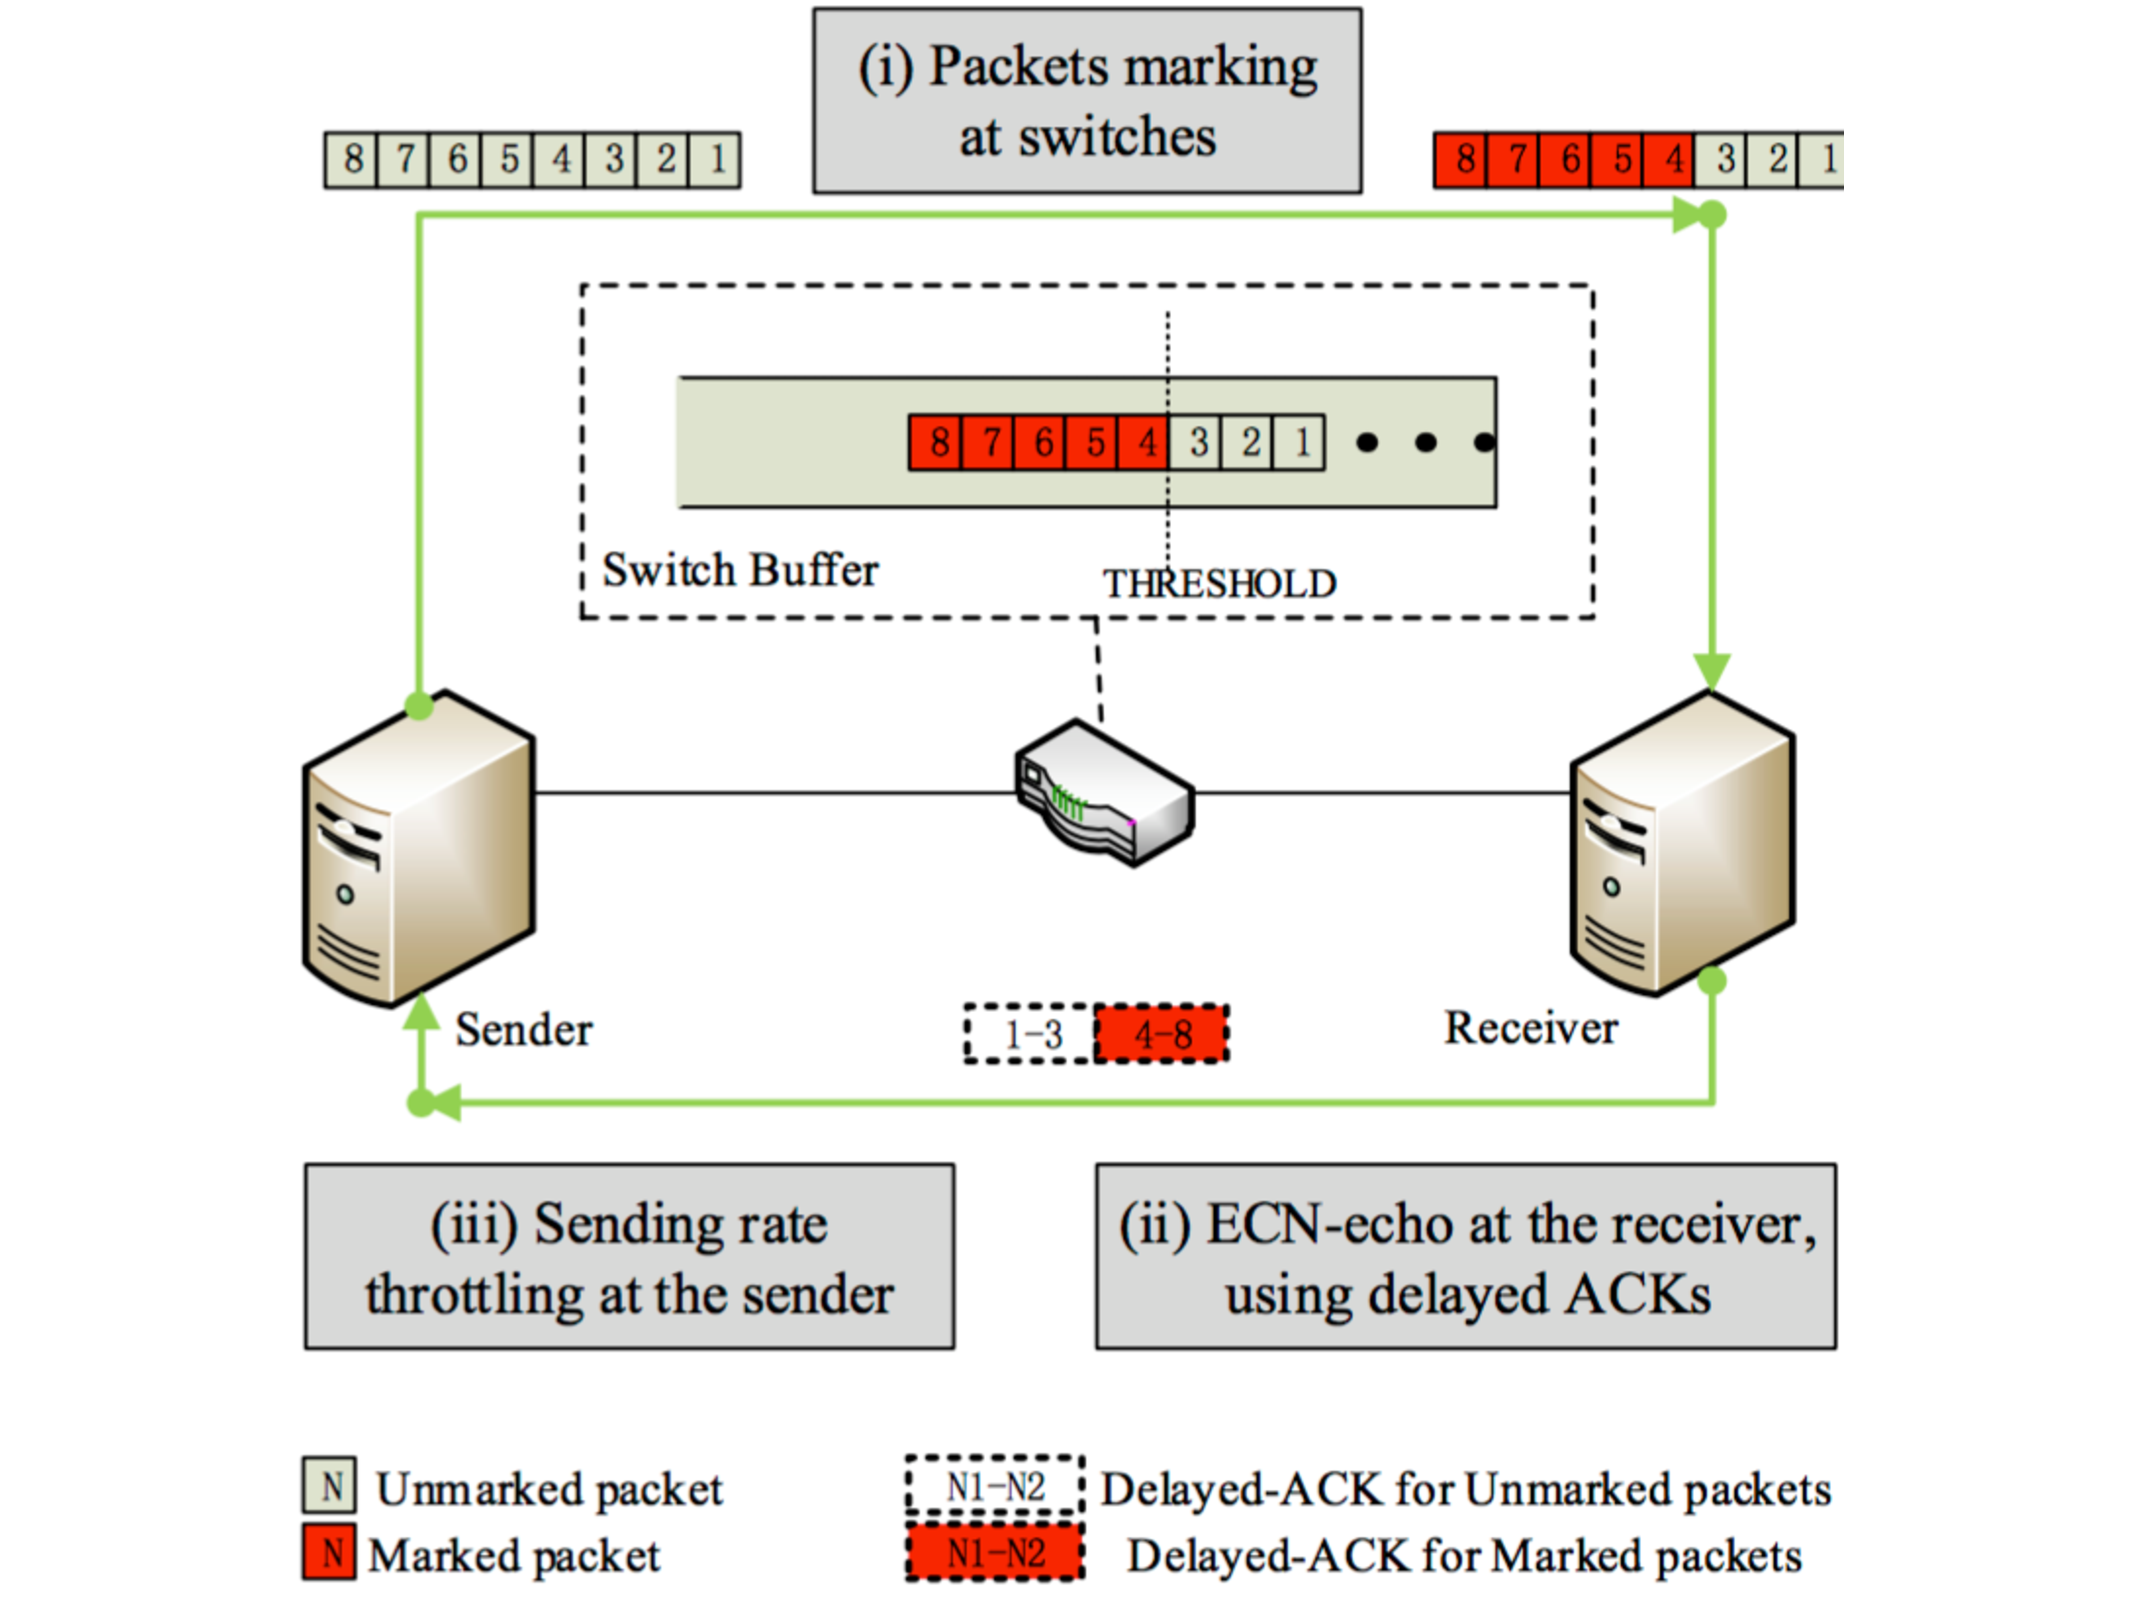
\includegraphics[width=0.9\columnwidth]{figures/others/model-process.pdf}
  \caption{基于ECN标记的数据中心速率控制过程,交换机上设置阈值,当排队队列超过阈值后,进行标记,发送端根据被标记的数据包比例,动态调整发送窗口}
  \label{model-process-fig}
\end{figure}

基于ECN标记的拥塞控制速率机制过程如图\ref{model-process-fig}所示:首先,发送端发送数据包给交换机,在交换机设置一个阈值,
当交换机队列长度超过阈值后,超过交换机设置队列设置阈值的数据包会被标记CE(和TCP不同,TCP会丢包)。
当接受端收到数据包后,检查数据包是否被标记CE,
如果发送的数据包被标记CE,那么给发送端回复的ACK中标记ECN。
发送端检查收到的ACK中被标记ECN的ACK的比例,以此来计算网络的拥塞程度$\alpha$,根据拥塞程度进行拥塞窗口的计算。

当网络中没有拥塞时(此RTT时间内没有被标记的数据包),滑动窗口每个RTT增加$(1-f_1(\alpha))$,
当网络中有拥塞时(此RTT时间内中有被标记的数据包),滑动窗口减小$f_2(\alpha)$倍。
其中$f_1(\alpha)$和$f_2(\alpha)$是关于拥塞程度$\alpha$的函数。
(\ref{Model-CA-eq})是基于ECN标记的拥塞避免阶段窗口变化的公式。

\begin{equation}
w=
\begin{cases}
w+(1-f_1(\alpha)) &\text{没有拥塞}\\
w \times (1-f_2(\alpha)) &\text{出现拥塞}
\end{cases}
\label{Model-CA-eq}
\end{equation}

\subsection{基于ECN标记流模型}\label{cha:model:introduction}
\begin{figure}[H] 
  \centering
  \includegraphics[width=0.9\columnwidth]{figures/others/senders.eps}
  \caption{N个发送端发送数据给1个接收端}
  \label{model-senders-fig}
\end{figure}

如图\ref{model-senders-fig}所示,假设N个发送端连接1个交换机,1个接收端连接在交换机上。
N个发送端使用公式(\ref{Model-CA-eq})进行拥塞控制窗口的计算。
交换机支持ECN标记,当交换机队列满足ECN标记条件时,发送到交换机的数据包会进行数据包标记。

公式(\ref{fluid-model_window})$\sim$(\ref{fluid-model-q})是基于ECN标记的描述模型,
其中(\ref{fluid-model_window})表示的是窗口变化过程,其中,第一部分$\frac{1-f_1(\alpha)}{R(t)}$描述的是窗口增加的过程,
其中每个RTT窗口增加$1-f_1(\alpha)$。
$\frac{w_i(t)f_2(\alpha)}{R(t)}p(t-R^*)$描述的是窗口减小的过程,当发生拥塞时,窗口减小$\frac{w_i(t)f_2(\alpha)}{R(t)}$。
其中$p(t-R^*)$表示的是否出现ECN标记,当$p(t-R^*)=1$时,表示ACK中有ECN标记,当$p(t-R^*)=0$时,表示ACK中没有ECN标记,
此时网络中没有拥塞。

公式(\ref{fluid-model_queue})表示的是交换机队列变化,
$ \sum_{i=1}^N{\frac{w_i(t)}{R(t)}}$表示的是发送到交换机的数据包,
假设交换机的转发速率是C pkt/s,那么,交换机的队列长度是$\sum_{i=1}^N{\frac{w_i(t)}{R(t)}}-C \label{fluid-model_queue}$。

公式(\ref{fluid-model-q})是交换机是否进行标记,当交换机队列满足一定条件$F({q}(t))==1$时,
进行标记的函数$\widehat{p}(t)=1$,否则,$\widehat{p}(t)=0$。
 \begin{align}
&\frac{dw_i}{dt}=\frac{1-f_1(\alpha)}{R(t)}-\frac{w_i(t)f_2(\alpha)}{R(t)}p(t-R^*)  \label{fluid-model_window} \\
&\frac{dq}{dt}= \sum_{i=1}^N{\frac{w_i(t)}{R(t)}}-C \label{fluid-model_queue}  \\
&\widehat{p}(t)=1_{F({q}(t))==1}  \label{fluid-model-q}
\end{align}




\subsection{LPD流模型}
假设N个并发的流通过容量为C pkts / sec的瓶颈链路传递给同一个接收者节点。
设置(\ref{Model-CA-eq})中$f_1(\alpha)=f_2(\alpha)=\alpha \times \frac{t}{t_{max}}$,
同时把$f_1(\alpha)$和$f_2(\alpha)$带入(\ref{fluid-model_window})$\sim$(\ref{fluid-model-q}),
并且增加$\alpha$标记方法,那么LPD流模型可以描述为:


 \begin{align}
&\frac{dw_i}{dt}=\frac{1-\alpha_i(t)\frac{t_i}{t_{max}}}{R(t)}-\frac{w_i(t)\alpha_i(t)\frac{t_i}{t_{max}}}{R(t)}p(t-R^*)  \label{LPD-model_window} \\
&\frac{d\alpha_i}{dt}=\frac{g}{R(t)}(p(t-R^*)-\alpha_i(t)) \label{LPD-model_alpha} \\
&\frac{dq}{dt}= \sum_{i=1}^N{\frac{w_i(t)}{R(t)}}-C \label{LPD-model_queue}  \\
&\widehat{p}(t)=1_{\widehat{q}(t)>1}  \label{LPD-model_mark}
\end{align}



其中,$w_i$表示$flow_i$的拥塞窗口的大小。 
$t_i$是$flow_i$的截止期限,$\alpha_i$表示$flow_i$的拥塞程度。 
q是交换队列长度,R表示RTT。
公式 (\ref{LPD-model_alpha}) 和 (\ref{LPD-model_mark})描述了交换机的ECN标记过程。
(\ref{LPD-model_window}) 模拟的是拥塞窗口。
公式(\ref{LPD-model_queue})描述交换机队列长度。
利用该模型,可以推算出窗口大小和队列长度。

\begin{figure}[h]
\centering
\subcaptionbox{窗口大小}
 {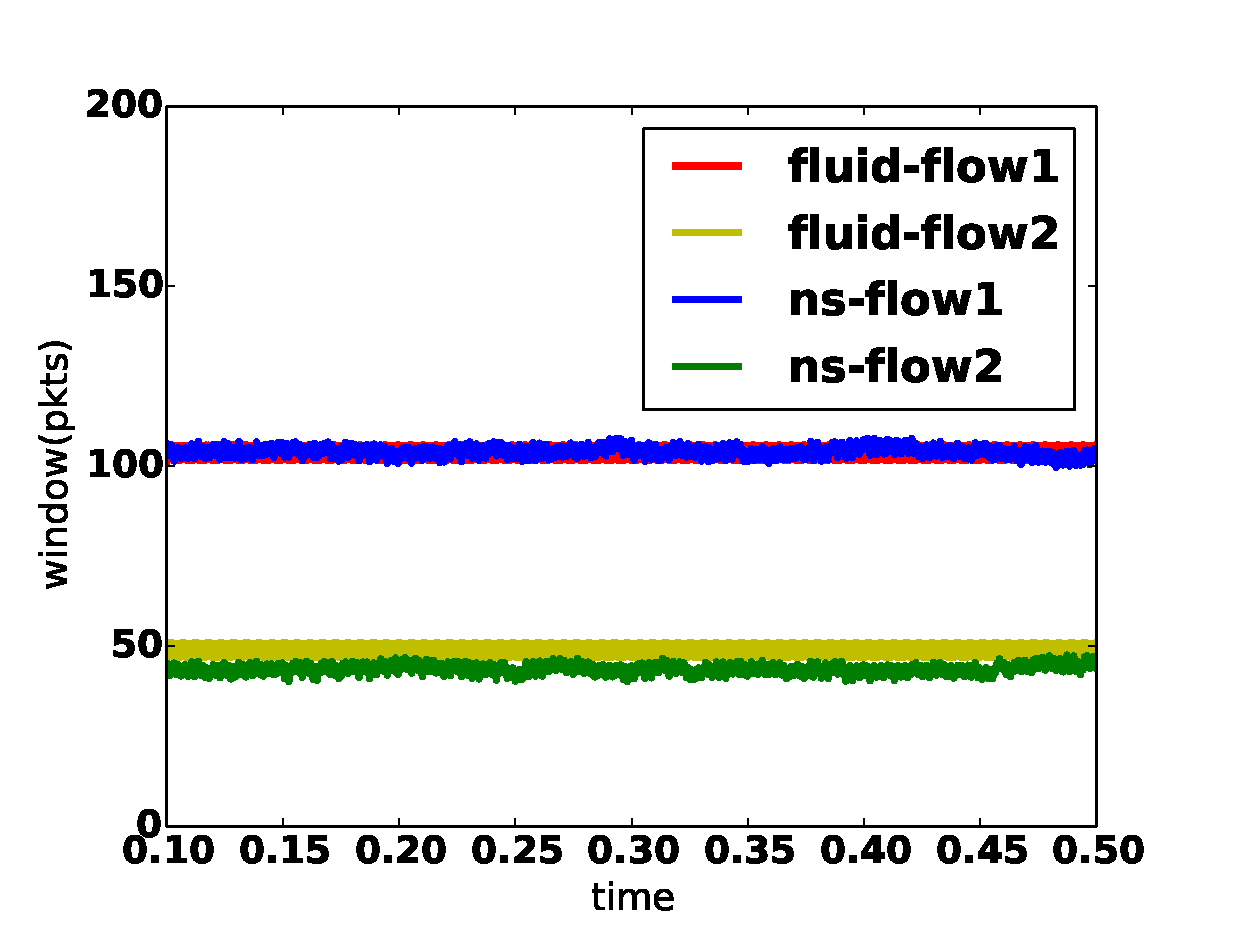
\includegraphics[width=0.32\columnwidth]{figures/LPD/2/window.eps}}
\subcaptionbox{队列长度}
{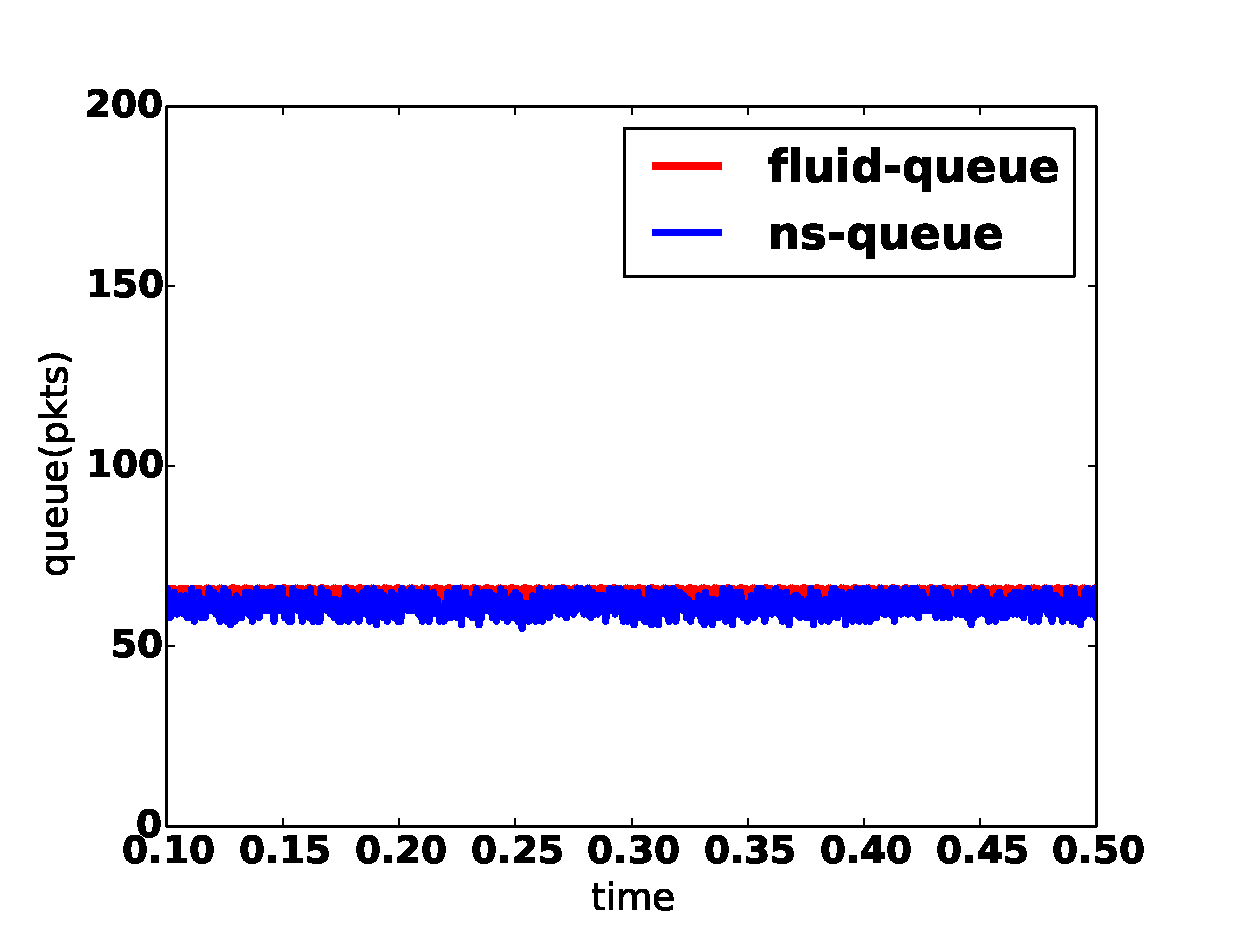
\includegraphics[width=0.32\columnwidth]{figures/LPD/2/queue.eps}}
\subcaptionbox{$\alpha$}
{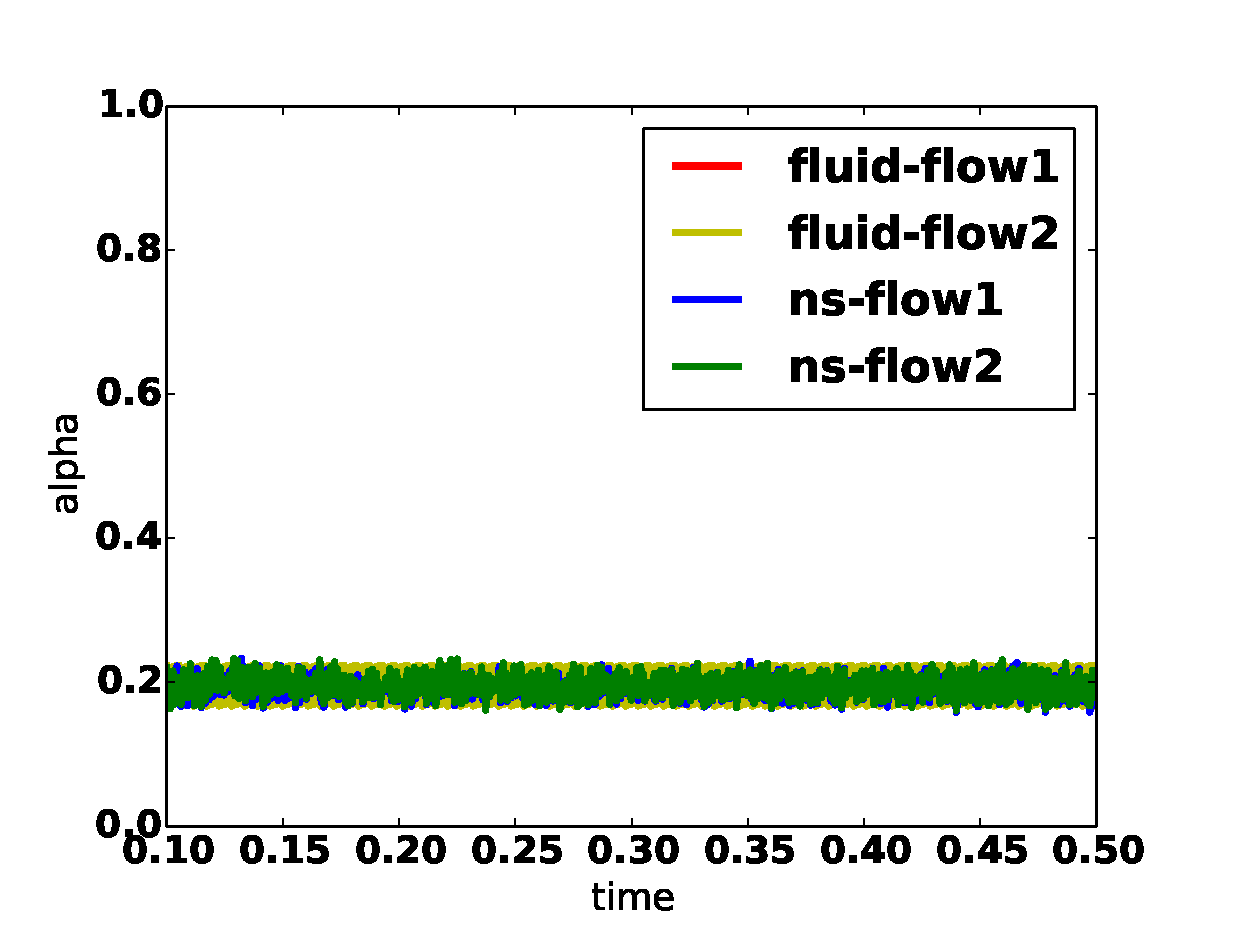
\includegraphics[width=0.32\columnwidth]{figures/LPD/2/alpha.eps}}
\caption{LPD 流模型和ns-2下结果对比}
\label{rate-analysis-fig}
\end{figure}


为了验证模型,启动两条长流,
期限分别是$t_1$ = 10s,$t_2$ = 20s,同时设置$t_{max}$ = 40s。
使用相同的参数在ns-2和流体模型下对比窗口大小,队列长度和拥塞程度。
窗口大小,队列长度和拥塞程度的仿真结果与模拟结果对比分别如图\ref{rate-analysis-fig}(a),
图\ref{rate-analysis-fig}(b)和图\ref{rate-analysis-fig}(c)所示。
可以看到使用流模型的推算结果和ns-2的模拟结果基本相符。



\begin{figure}[h]
\centering
\subcaptionbox{单条流的带宽}
 {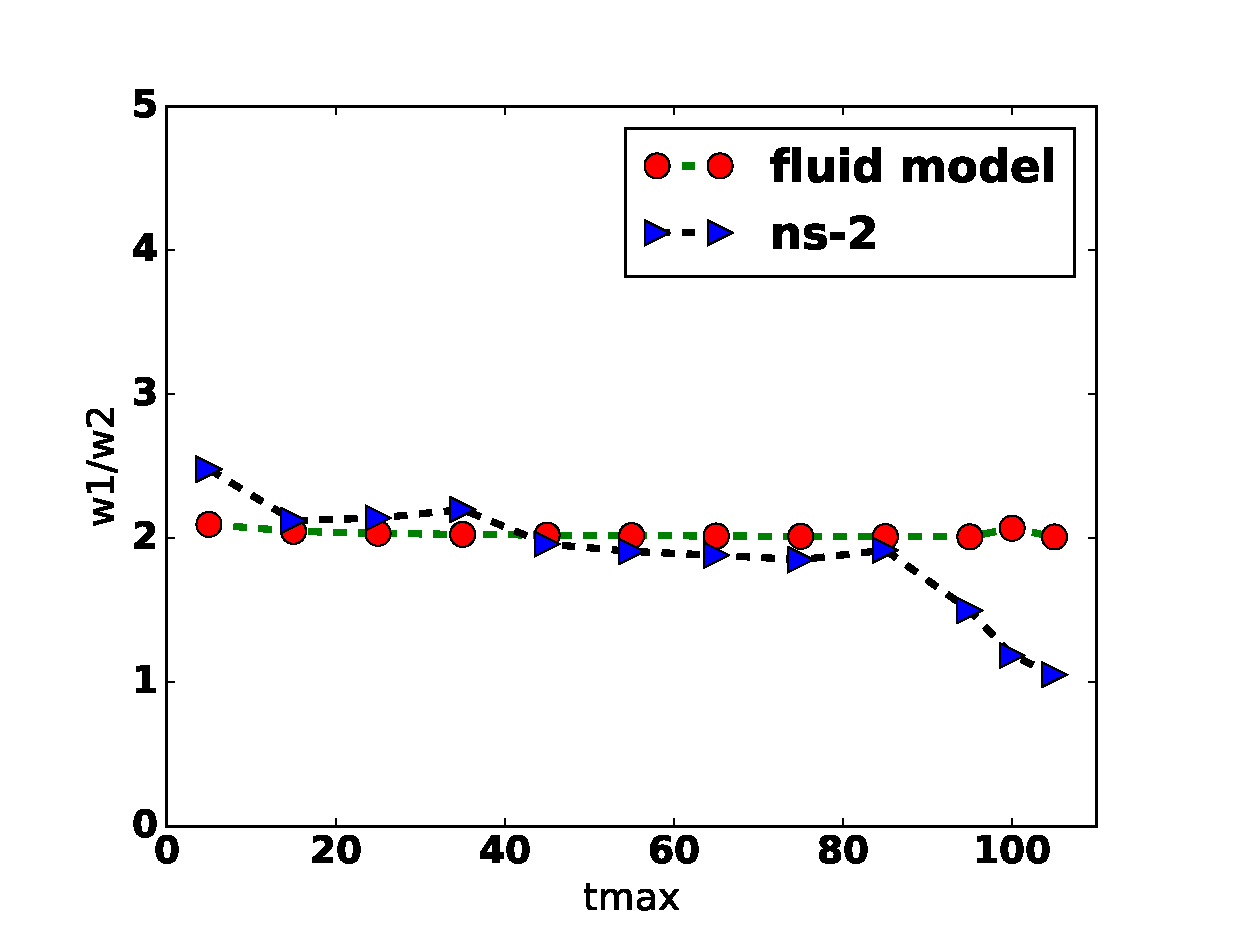
\includegraphics[width=0.45\columnwidth]{figures/LPD/parameter/ratio.eps}}
\subcaptionbox{$pd=p(\alpha, d_{1})-p(\alpha, d_{2})$}
{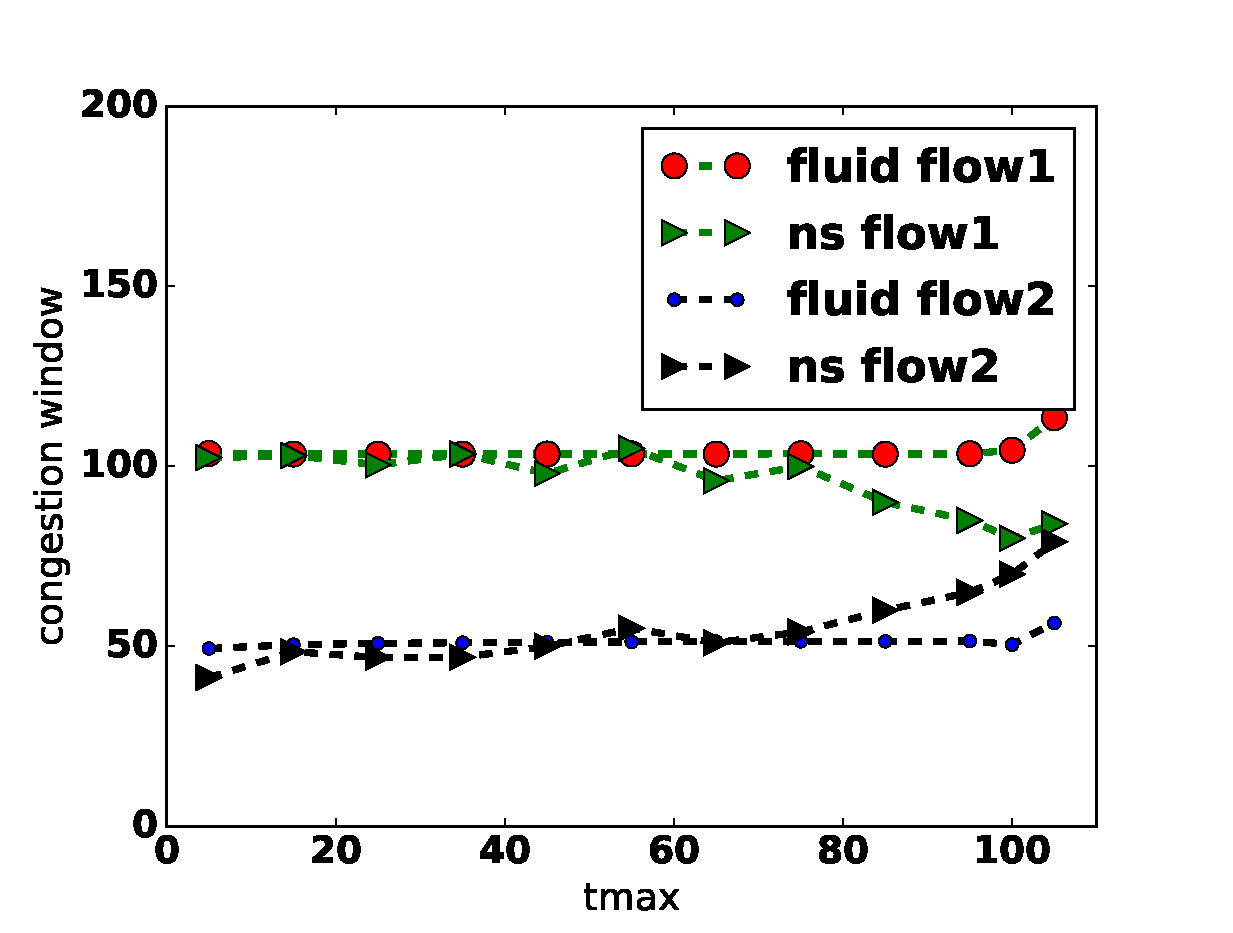
\includegraphics[width=0.45\columnwidth]{figures/LPD/parameter/window2.eps}}
\caption{LPD-t下的两条流}
\label{rate-ratio-fig}
\end{figure}



为了进一步测试模型的准确性,
启动两条长流,设置瓶颈带宽是10Gbps,两条流的期限分别是$t_1$ = 0.5 s,$t_2$ = 1s。
设置数据包大小为1500B,RTT为100 us,K为64。
图\ref{rate-ratio-fig}显示了模拟结果和ns-2方针结果的对比。
从图\ref{rate-ratio-fig}(a)可以看出,当$t_{max} <100$时,流模型和ns-2仿真的结果都是$w_1 /w_2 \approx 2$。
然而,当$t_{max}> 100$时,ns-2模拟的$w_1\approx w_2$和流模型的$w_1 /w_2 \approx  2$。
图\ref{rate-ratio-fig}(b)表明当$t_{max}> 100$时,流模型会推算出较大的拥塞窗口。
此表明,$t_{max}$在实际中应该被设置适当值,下面讨论在实际中如何$t_{max}$。



\subsubsection{$t_{max}$的选择}
在LPD流模型中,流具有不动点$(w_i,\alpha_i)=(t_{max}-t_i,1)$。
不动点的实际意义是所有数据流的$\alpha= 1$。
即重度拥塞的情形下,所有的数据包都被标记,所有流拥有固定的拥塞窗口。
在LPD中,$t_{max}$应该选择适当的值。
下面分析$t_{max}$取值:

假设有N条流$(t_{max}> t_1> t_2> ...> t_n)$同时启动,
其中,$t_1$$\sim$$t_n$是流flow$_1$$\sim$flow$_n$的截止期限。
在时刻t,队列长度表示为q(t),则有:

\begin{equation}
\label{tmaxprocess}
\frac{t_{max}-t_1}{t_1}+\frac{t_{max}-t_2}{t_2}+...+\frac{t_{max}-t_n}{t_n} <q(t)+C\times RTT
\end{equation}



假设当交换机队列超过K时,数据包开始标记。
那么,对于N条数据流,每个RTT,拥塞窗口大小不超过1。
那么我们有$q(t) < K+N$。因为我们假设$t_{max}>t_1>t_2>…>t_n$,因此有:


\begin{equation}
\label{tmax}
t_{max}<\frac{t_1\times(K+C\times RTT+2N)}{N}
\end{equation}

根据(\ref{tmax}),可以根据截止期限的最大值,最大并发流量数量,
RTT和瓶颈链路链接带宽来设置$t_{max}$。 
在当前数据中心,设置C为10Gbps,数据包大小为1500B,RTT为100us,
因为数据中心,大多数情况下并发连接数小于100 \cite{DCTCP},假设设置K为60:


 \begin{equation}
\label{tmax_suggest}
t_1< t_{max}<3.5\times t_1
\end{equation}

在实际部署LPD时,可以根据(\ref{tmax})计算$t_{max}$。(\ref{tmax_suggest})可以当作 $t_{max}$的缺省值。
事实上,结果与图\ref{rate-ratio-fig} (b)一致。 
根据(\ref{tmax_suggest}),当$N = 2$时,$t_{max}\le76* t_1$。
在此情况下,$t_1 = 1s$, 从ns-2仿真中可以看出,当$t_{max}> 80$时,流拥塞窗口不再与其对应的t成反比。

\subsubsection{K的设置}
实际中,交换机的阈值K不可设置的过大或者过小,否则,链路利用率会很低。
在实际部署LPD时,需要使链路利用率达到$100\%$。
因此需要确定阈值K的设置范围\cite{DCTCPAnalysis}。

qmin,qmax表示交换机队列的最小和最大长度。
基于ECN标记的拥塞控制策略,队列长度在固定区间内波动。
阈值K应大于下冲振荡(否则队列大小将为零,链路利用率将不是$100\%$)。 
使用LPD流模型,并将流的期限设置在10以内,将$t_{max}$从10变为55,
并将链路带宽从1Gbps变为10Gbps。 
最后,针对每一个$t_{max}$我们记下每组队列下限的最小值。
结果如图\ref{qmin-fig}所示。
可以看到g值很小,即使是最坏的情形($t_{max} = 55$, $t_{max}\simeq 5 t_1$),也可以得到:
\begin{equation}
\label{KRANGE}
K \gtrapprox0.4 CR
\end{equation}


\begin{figure}
\begin{minipage}{0.5\textwidth}
  \centering
  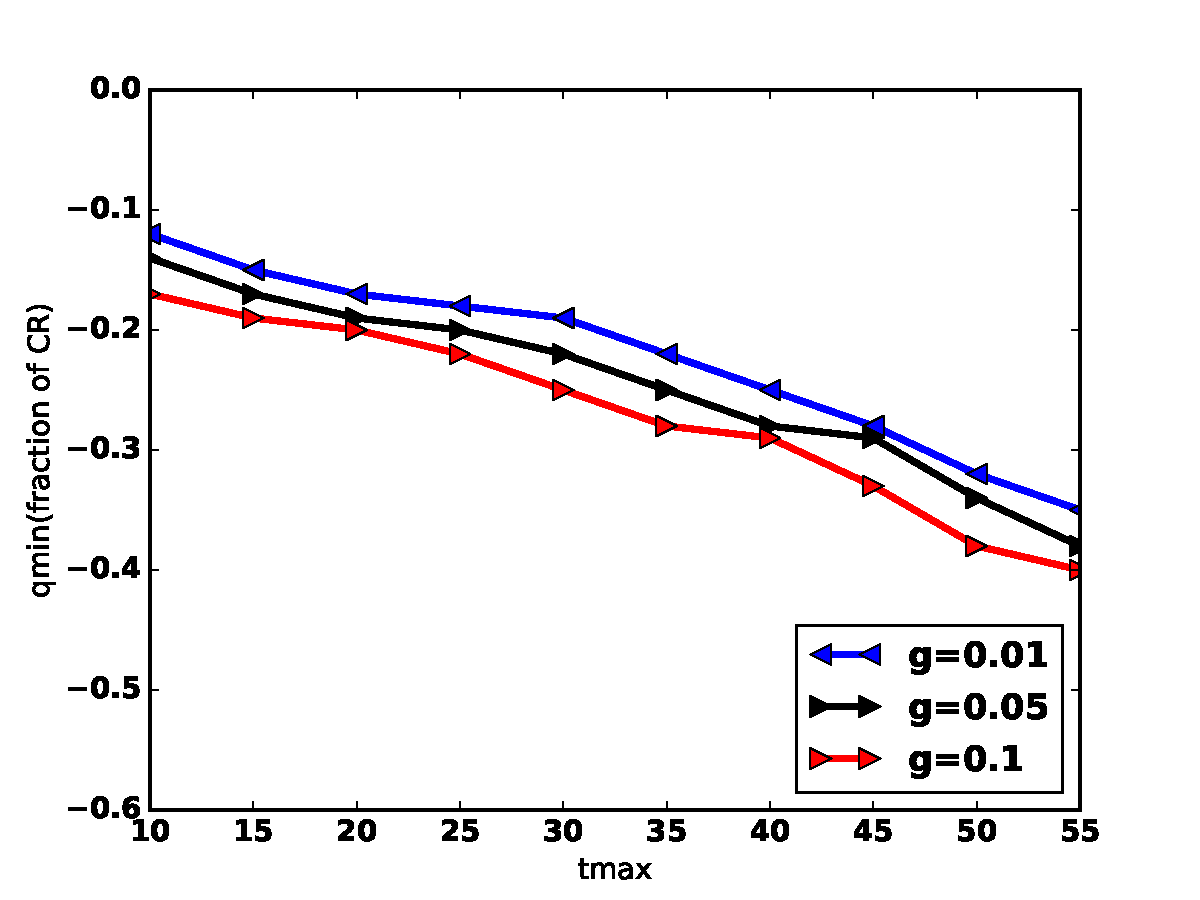
\includegraphics[width=0.7\columnwidth]{figures/LPD/model/qmin.pdf}
  \caption{队列最小长度波动}
  \label{qmin-fig}
\end{minipage}
\begin{minipage}{0.5\textwidth}
  \centering
  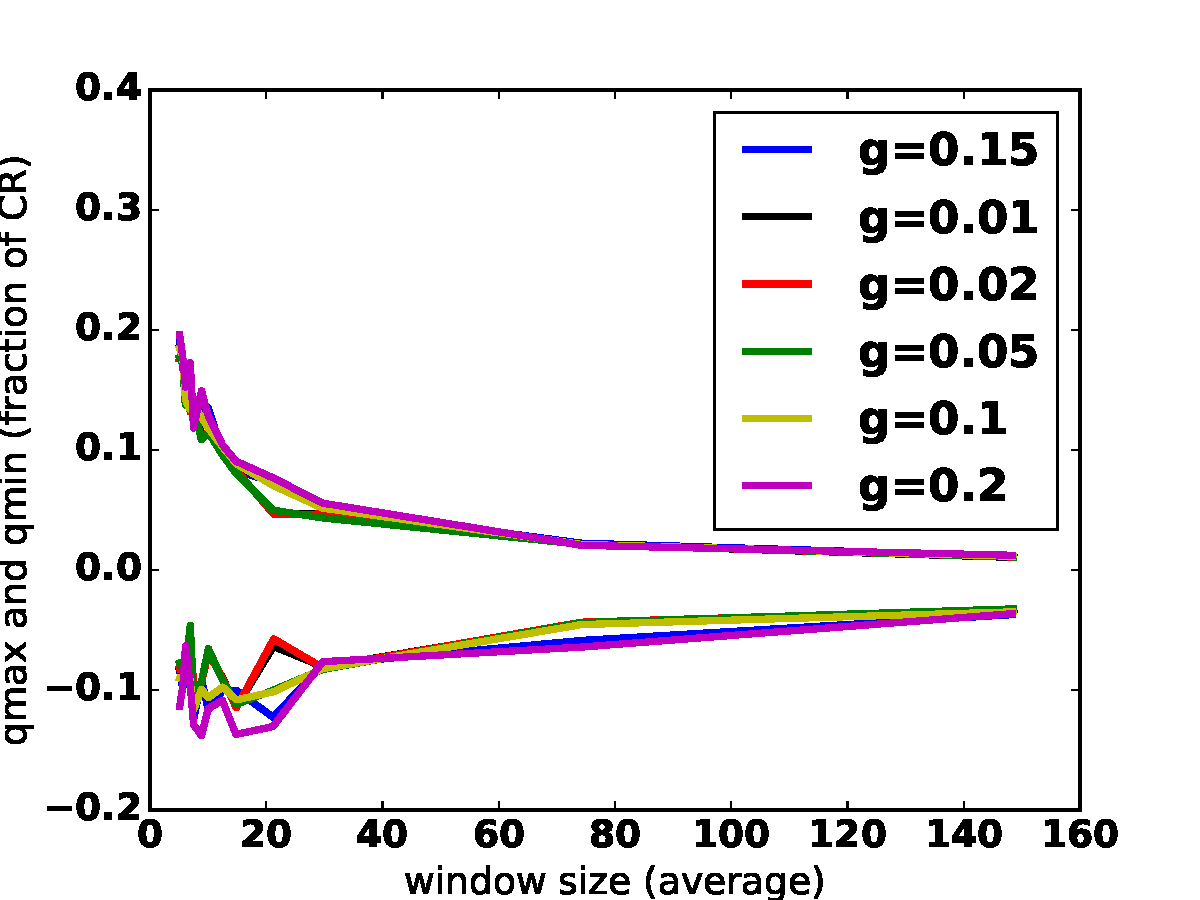
\includegraphics[width=0.7\columnwidth]{figures/LPD/model/k.pdf}
  \caption{队列最大和最小}
  \label{k-fig}
\end{minipage}
\end{figure}

\begin{figure}[H] 
  \centering
  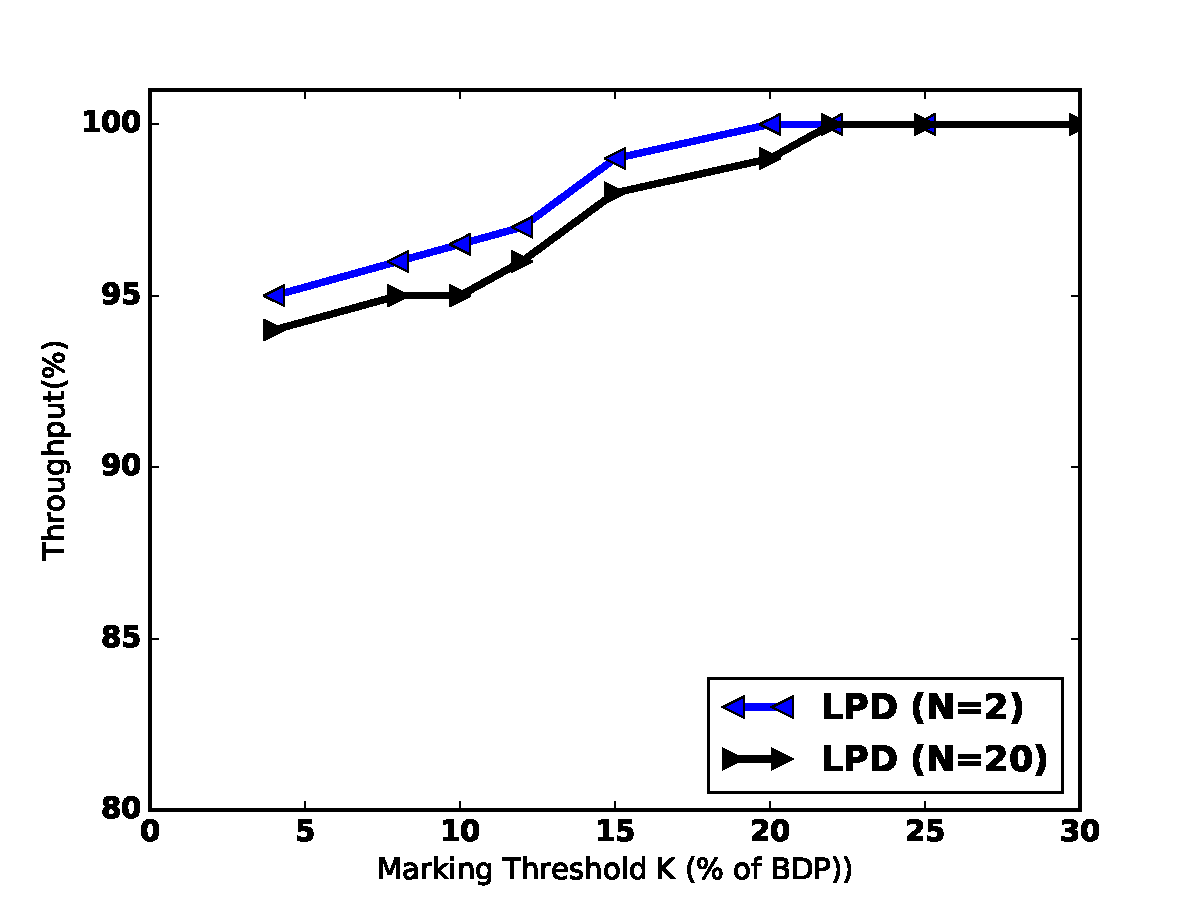
\includegraphics[width=0.6\columnwidth]{figures/LPD/model/throughput.pdf}
  \caption{ns-2仿真中吞吐量和标记阈值K的关系。从4到30个包(BDP的$2.4-18\%$)变化。 
结果表明,即使对于小于BDP的$3\%$的K,吞吐量仍然高于$95\%$}
  \label{throughput-fig}
\end{figure}


至于RTT,因为$R = d + K / C$,将R带入(\ref{KRANGE}),
所以在最坏的场景下,得到队列的缺省值0.67Cd。 
假设链路带宽是C =10Gbps,链路传送延迟d=100us,数据包大小是1500B,则K至少应该设置为56。
对于数据中心中常见的情形,链路传播延迟为100us,链路的瓶颈带宽为10Gbps。
设置$t_{max} = 10$,截止期限在1到10范围内随机生成。
使用LPD流模型,图\ref{k-fig}显示了flow$_1$,使用不同的g值下平均窗口大小与qmin和qmax(其中qmin表示队列最小值,qmax表示队列最大值,qmin和qmax换算成CR)的关系图。
可以看到$K\gtrapprox0.12CR$。
为了避免队列下溢,需要有$K > |qmin |C*R \simeq0.12CR$。  
由于$R=d+K/C$,因此可以得到:
\begin{equation}
\label{KVALUE}
K \simeq 0.14 Cd
\end{equation}

换言之,大约需要$14\%$的BDP就能实现链路利用率达到$100\%$。 
多余的缓冲区可以用来处理突发流。
为了测试上面的实验结果,图\ref{throughput-fig}显示ns-2仿真中吞吐量和标记阈值K的关系图。 
在这个实验中,变换K的取值从4到30(大约是BDP的$2.4\% \sim18\%$)。 
结果表明,ns-2仿真结果与LPD流模型相似,即使当K设置小于$3\%$倍的BDP时,吞吐量仍然高于$95\%$。 
 
\section{实验验证}\label{LPDevaluation}
本节通过ns-2 \cite{ns2}仿真和实际测试床来评估LPD的性能。 
本文根据DCTCP网站\cite{DCTCPcode}发布的DCTCP的源代码实现了LPD(包括LPD-t,LPD-e),
并将Vamanan\cite{D2TCP}提供的D$^2$TCP的ns-3代码移植到ns-2。 
另外,本文的实验同时实现L$^2$DCT,Karuna,并改动pFabric的代码到ns-2平台上。 
本文所有代码均可以在LPD开源代码网站\cite{LPD-sim-code}下载。 
同时本文的实验也在Linux内核3.2.61中实现了LPD,D$^2$TCP,L$^2$DCT,
并在真实环境上作评估,相应的源代码可以在LPD内核代码网站\cite{LPD-code}下载。

\subsection{LPD重度负载下性能验证}

%
\begin{figure}[h]
\setlength{\abovecaptionskip}{0pt} 
\setlength{\belowcaptionskip}{1pt} 
  \centering%
  \subcaptionbox{流的带宽\label{LPD_Evaluation_Motivation:subfig1}} 
    {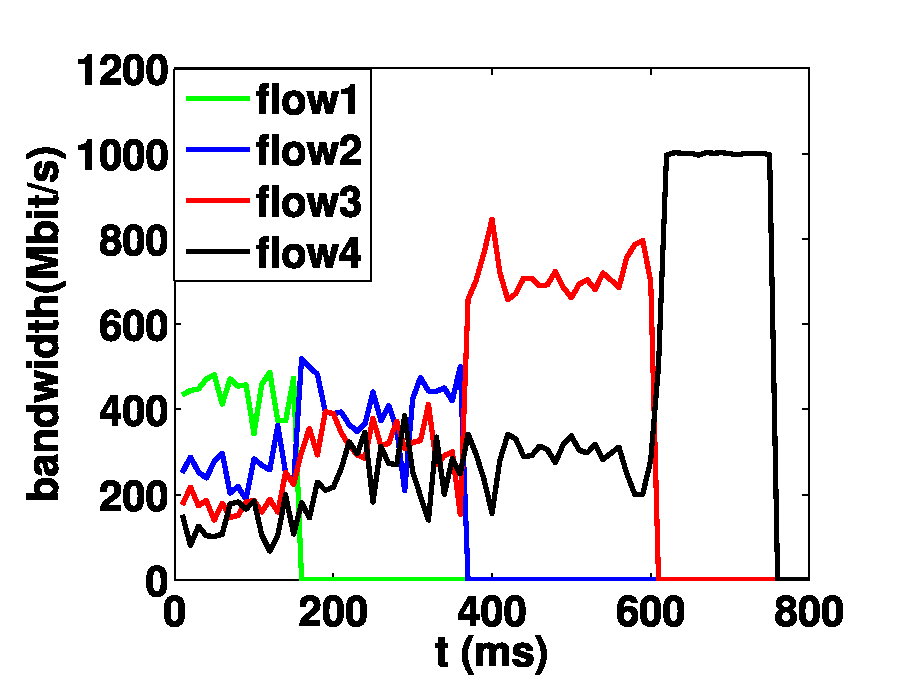
\includegraphics[width=0.45\columnwidth]{figures/LPD/evaluation_1/LPD_bandwidth2.eps}\quad}
  \subcaptionbox{拥塞窗口\label{LPD_Evaluation_Motivation:subfig2}}
      {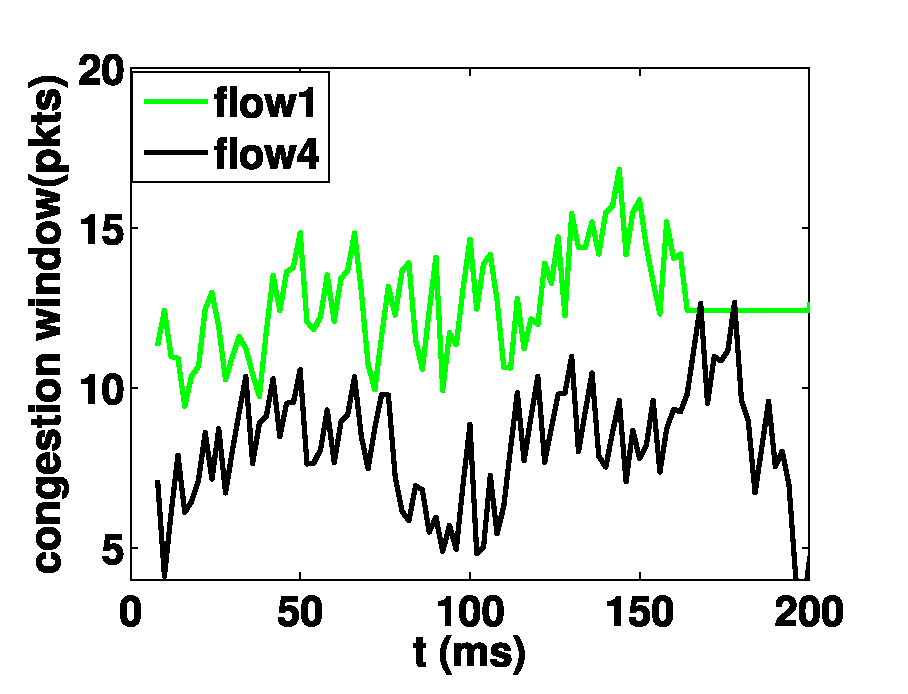
\includegraphics[width=0.45\columnwidth]{figures/LPD/evaluation_1/LPD_window2.eps}\quad}
  \subcaptionbox{flow$_1$和flow$_4$的期限因子\label{LPD_Evaluation_Motivation:subfig3}}
    {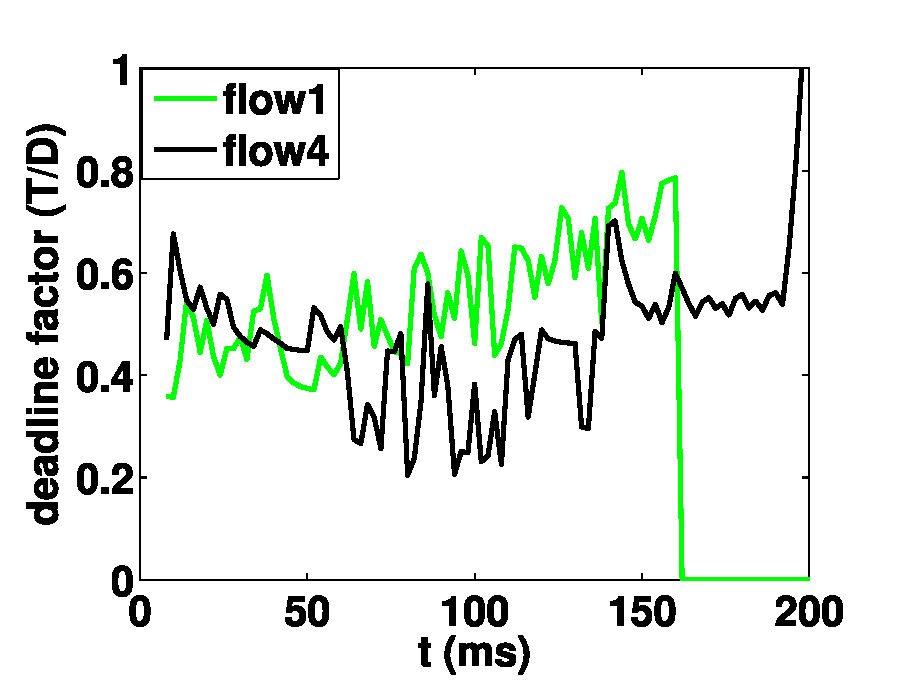
\includegraphics[width=0.45\columnwidth]{figures/LPD/evaluation_1/LPD_factor2.eps}\quad}
  \subcaptionbox{flow$_1$和flow$_4$的拥塞程度\label{LPD_Evaluation_Motivation:subfig4}}
      {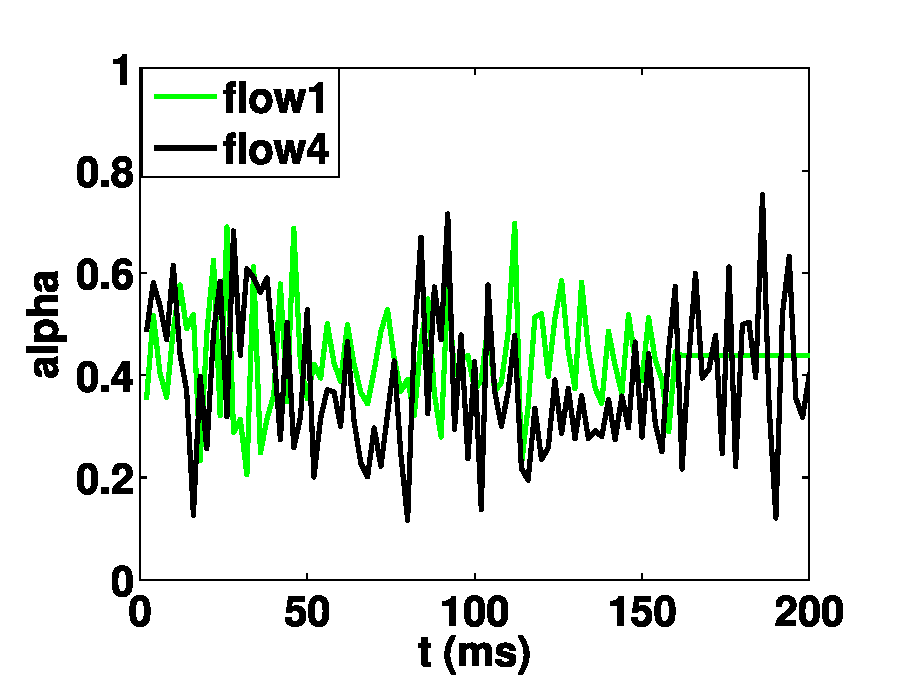
\includegraphics[width=0.45\columnwidth]{figures/LPD/evaluation_1/LPD_alpha2.eps}\quad}
  \caption{LPD下4条流的性能,使用和 D$^{2}$TCP相同的参数}
  \label{evalution_cases_principle_fig}
\end{figure}



\begin{figure}[h]
\setlength{\abovecaptionskip}{0pt} 
\setlength{\belowcaptionskip}{1pt} 
  \subcaptionbox{流的带宽\label{LPD_Motivation:subfig3}} [0.5\linewidth]  
    {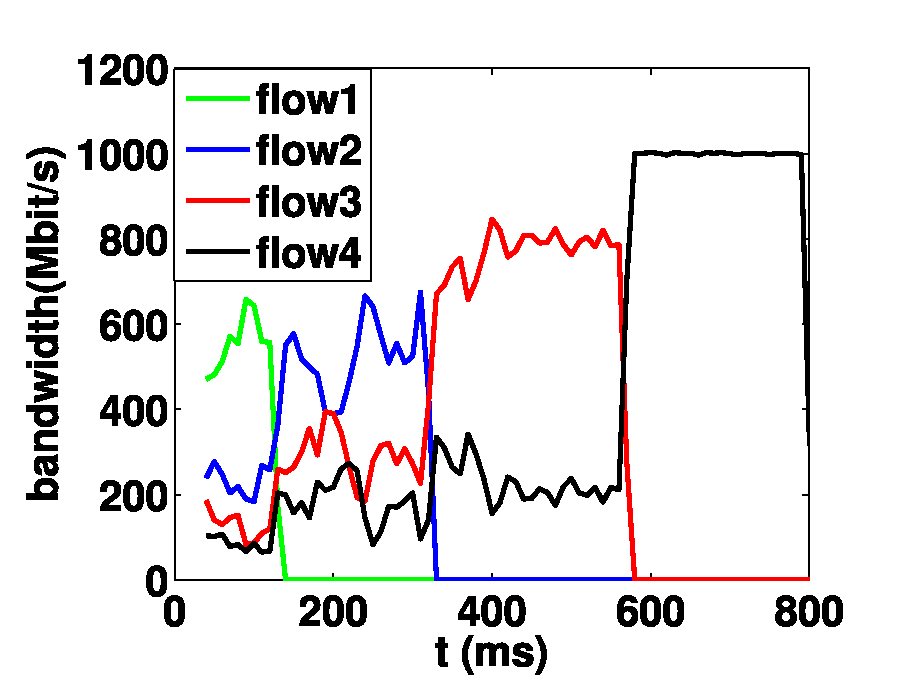
\includegraphics[width=0.5\columnwidth]{figures/LPD/evaluation_1/LPD_bandwidth.eps}}
  \subcaptionbox{拥塞窗口\label{LPD_Motivation:subfig4}}[0.5\linewidth]  
      {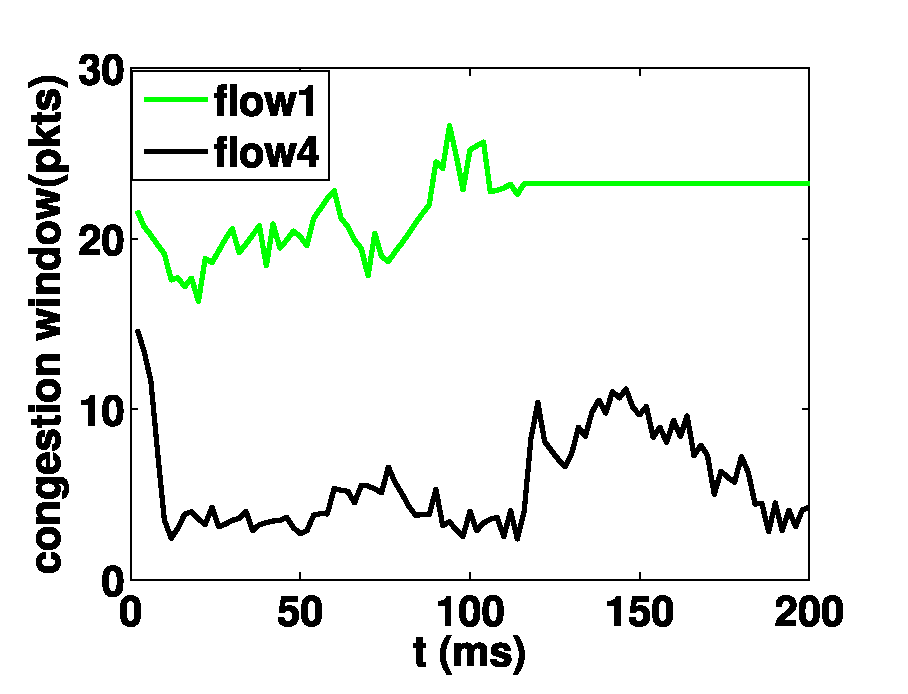
\includegraphics[width=0.5\columnwidth]{figures/LPD/evaluation_1/LPD_window.eps}}
  \subcaptionbox{交换机队列长度\label{LPD_Motivation:subfig5}}[0.5\linewidth]  
    {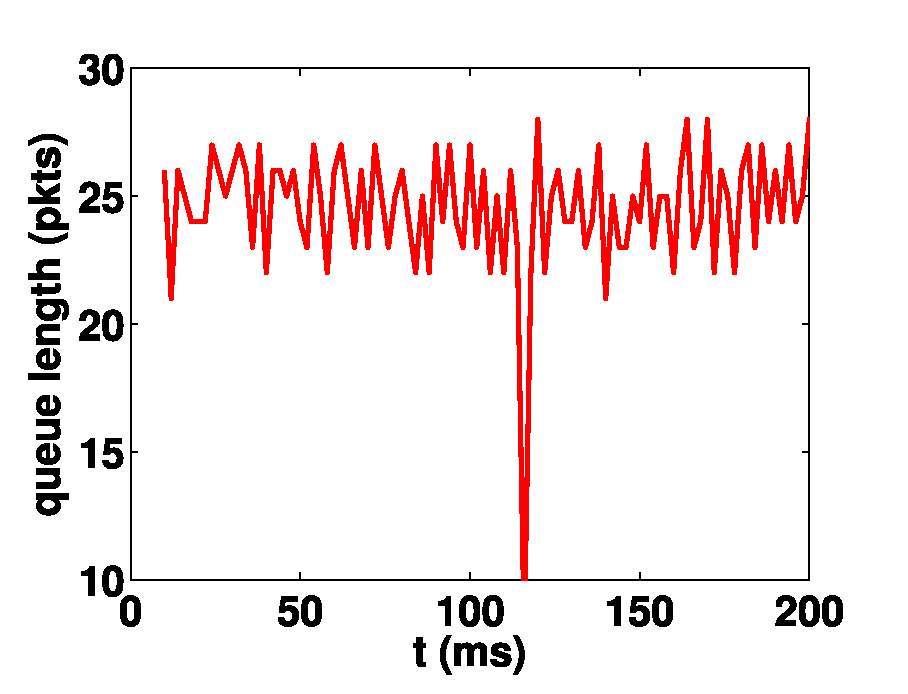
\includegraphics[width=0.5\columnwidth]{figures/LPD/evaluation_1/LPD_queue.eps}}
  \subcaptionbox{flow$_1$和flow$_4$的拥塞因子\label{LPD_Motivation:subfig6}}[0.5\linewidth]  
      {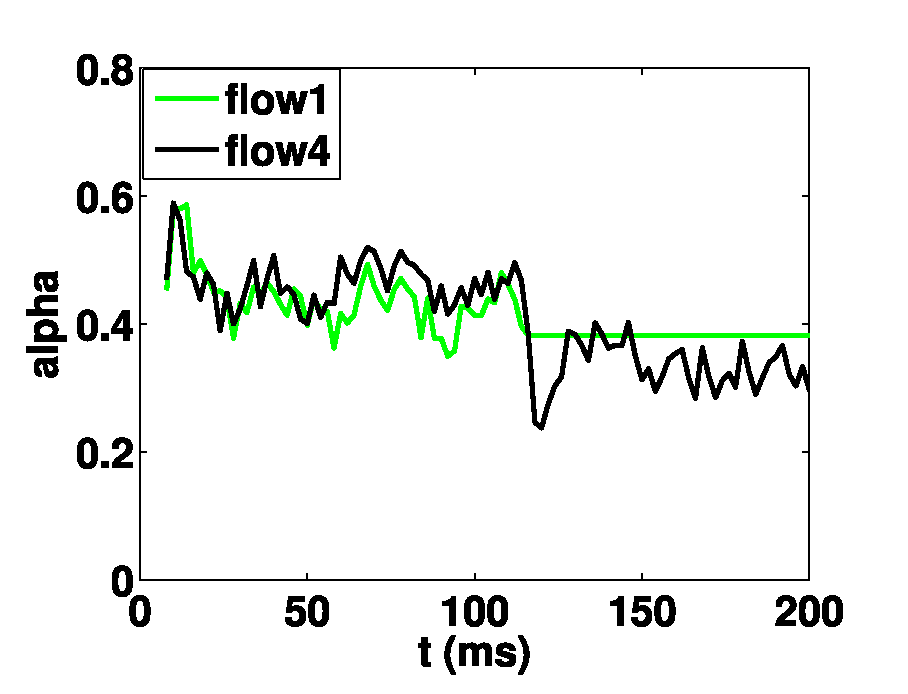
\includegraphics[width=0.5\columnwidth]{figures/LPD/evaluation_1/LPD_alpha.eps}}
  \caption{LPD-t下4条流的性能,使用和 D$^{2}$TCP相同的参数}
  \label{evalution_cases_fig}
\end{figure}



本文首先将LPD应用到\ref{sec_LPD:Motivation}节研究动机介绍的实例中。
虽然此例不是一个典型的OLDI场景,
但是可以用它来检查LPD是否能够帮助更多的流量达到最终期限,
特别是在负载较重的情况下测试LPD的性能。
使用与D$^2$TCP相同的期限因子d=T/D,改动LPD,称之为LPD-d。
在相同的设置下,如图\ref{evalution_cases_principle_fig}(a)所示,只有flow$_2$在LPD-d下错失期限(deadline),
为了更好地理解LPD优于D$^2$TCP和DCTCP的原因,
我们在图\ref{evalution_cases_principle_fig}中给出了LPD下流状态的更多细节。


图\ref{evalution_cases_principle_fig}显示每条流的带宽,以及拥塞窗口w,
期限因子d和flow$_1$与flow$_4$的网络拥塞程度$\alpha$的情形。
与图\ref{LPD_Motivation}对比可以看出,随着流发送,
flow$_1$和flow$_4$之间拥塞窗口之间的差异变得更大,而flow$_1$和flow$_4$的期限因子和网络负载变化不大。
这是因为选择正比负载差分策略,当网络拥塞程度增加时,flow$_1$和flow$_4$有更大的带宽分配差异。
如图\ref{evalution_cases_principle_fig}(a)所示,最终,LPD-d比D$^2$TCP错过期限的流的数目更少。



为了进行比较,设置$t_{max}$ = 800ms,并且在相同的实验环境中测试LPD-t。
如图\ref{evalution_cases_fig}(a)所示,使用LPD-t,所有流在截止期限之前完成传输,
这是因为使用LPD-t,截止时间更近的流会获得更多的带宽,
例如有带宽大小关系:flow$_1>$flow$_2>$flow$_3>$flow$_4$。
图\ref{evalution_cases_fig}描述了LPD-t内部状态,
与LPD-d和D$^2$TCP相比,
如图\ref{evalution_cases_fig}(c)与图\ref{evalution_cases_fig}(d)所示,尽管流计算出的网络负载(即每条流计算的$\alpha$值)基本相同,
但如图\ref{evalution_cases_fig}(d)所示,不同截止期限的数据流的拥塞窗口差异很大。
例如,在前200 ms时间内,flow$_1$获得约$55\%$的带宽,而flow$_4$仅获得$10\%$的带宽。
图\ref{evalution_cases_fig}(c)显示在开始200ms时间内交换机的队列长度,
可以看到,交换机的队列在阈值$K = 25$附近表现出小的波动。
队列在128$ms$处突然下降是由于flow$_1$在此时间点完成传输,
此后,队列很快被未传输完成的数据包填充,
由此还可以看到LPD数据流可以很快的填充交换机队列,从而充分利用链路带宽。
\begin{figure}[H] 
  \centering
  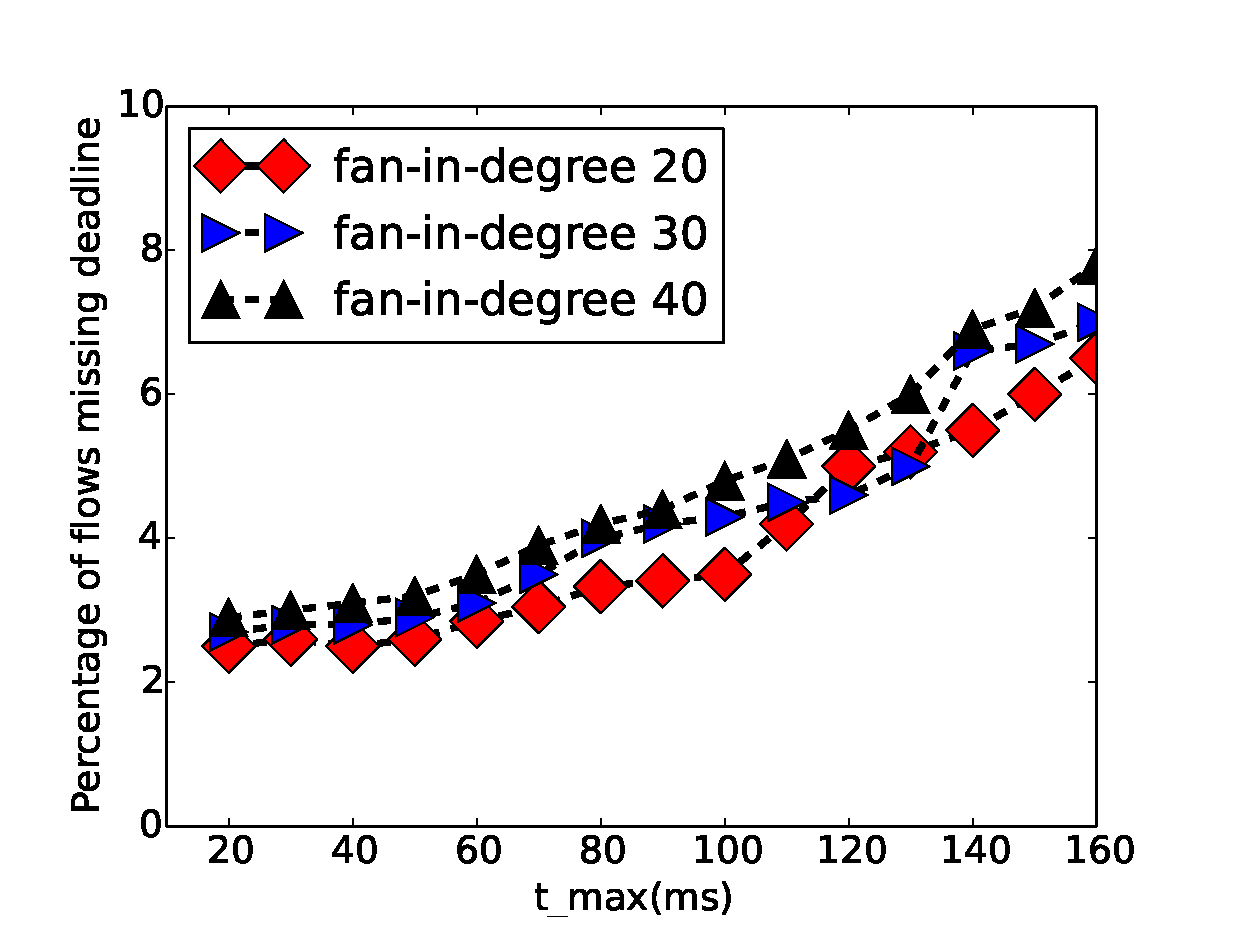
\includegraphics[width=0.8\columnwidth]{figures/LPD/evaluation_3/DMAX.eps}
  \caption{变化 $t_{max}$的影响}
  \label{tmax-fig}
\end{figure}

\subsection{参数选择}
LPD-t和LPD-e必须设置适当的上限$t_{max}$和$s_{max}$。
此处本文只讨论$t_{max}$,因为$s_{max}$有类似的作用。
从LPD-t的等式(\ref{LPD-t-eq})可以看出如果$t_{max}$变大,惩罚函数f就变小。
从(\ref{tmax}),得知对于C = 1Gbps,K = 25,RTT = 1ms,最大数据包大小为1500B,
当并发数据流数量为20,30,40时,对应的$t_{max}$应小于$6 * t_1$,$4 * t_1$,$3 * t_1$。
如果$t_{max}$太大,区分不同期限的流的能力也变弱。
使用OLDI应用来检查$t_{max}$对LPD-t的性能影响,
其中流的截止期限都设置在20ms内,
变换$t_{max}$从20ms变化到160ms(即$t_1 <t_{max} <8 * t_1$)。
图\ref{tmax-fig}描述了不同$t_{max}$下错失期限的流数目,
而扇入度(fan-in-degree,即同时到达根节点的流的数目)分别是20,30和40。


从图\ref{tmax-fig}可以看出,
当$t_{max} $<80ms时,即$t_{max}$不超过最大截止期限的4倍时,使用LPD-t,少于$5\%$的流错过截止期限。
LPD-t的性能总是比D$^2$TCP优异(D$^2$TCP在扇入度分别是20,30和40时错过期限的比例分别为$3.45\%$,$4.96\%$和$5.45\%$)。
而且在这个范围内,使用不同$t_{max}$,LPD的性能差异较大。
然而,当$t_{max}$很大时,例如,当$t_{max}>$120ms(即6倍于截止期限)时,
LPD-t的性能较差,并且比D$^2$TCP差,这和之前推倒结果相符。


\subsection{仿真测试}

\subsubsection{简单拓扑测试}
\begin{figure}[H] 
  \centering
  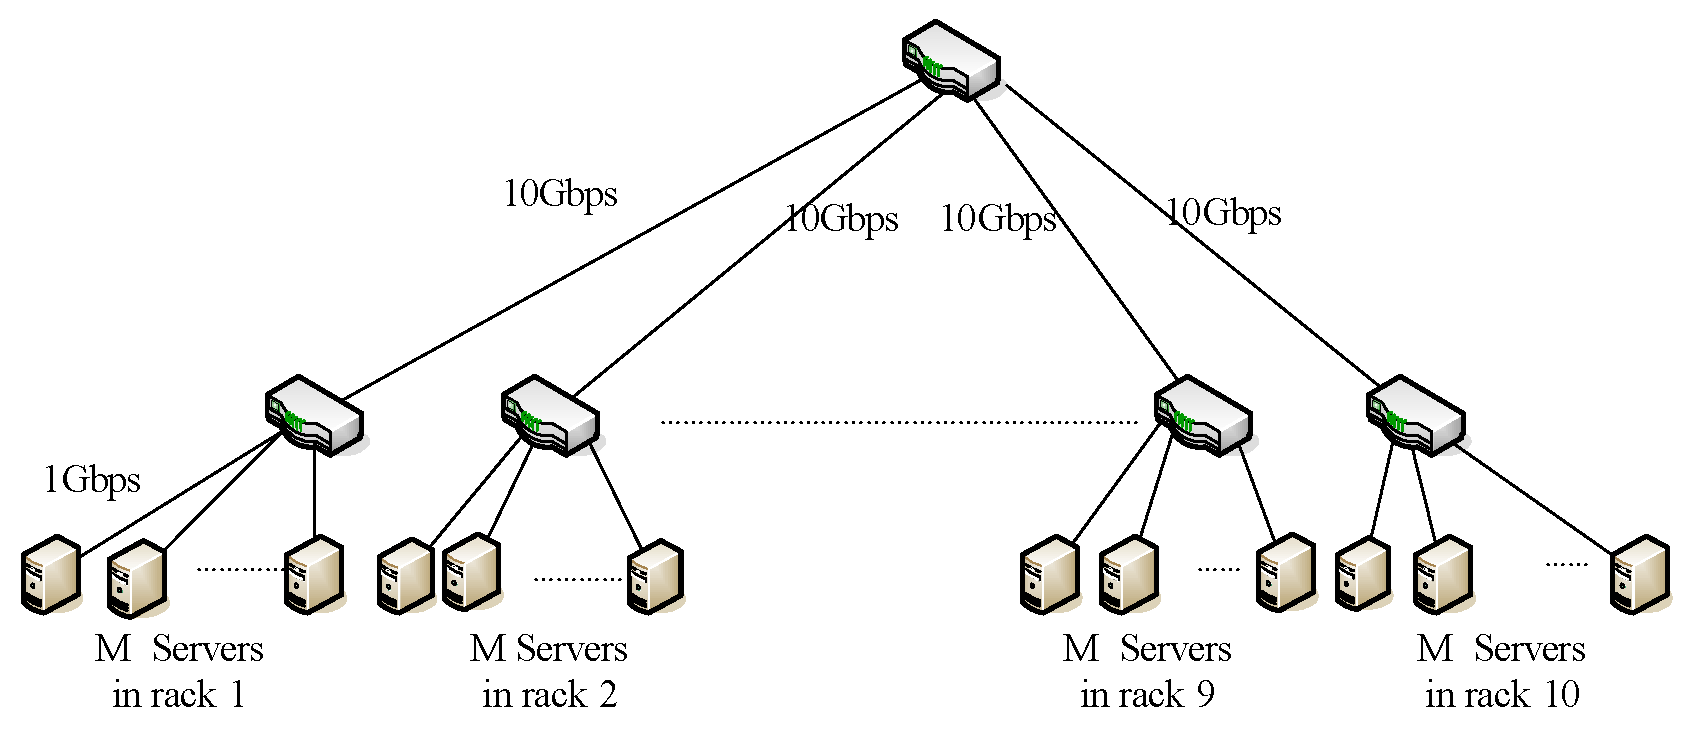
\includegraphics[width=0.9\columnwidth]{figures/LPD/DataCenter.eps}
  \caption{简单的数据中心拓扑}
\label{DataCenterTop-fig}
\end{figure}

为了测试在数据中心下LPD-e的性能,构建一个如图\ref{DataCenterTop-fig}所示的三级树形拓扑。
这个拓扑有10个机架,每个机架由M = 40个服务器组成,机架连接到顶层的TOR交换机。
服务器和交换机之间的链路带宽为1Gbps。
所有TOR交换机通过10Gbps链路连接到根交换机。

和\inlinecite{DCTCP,D2TCP,L2DCT}类似,设置交换机的标记阈值K=20,并将传播延迟d设置为100us。 
TCP重新传输超时(RTO)设置为10ms,每个发送端初始拥塞窗口设置为12。
考虑在数据中心内,很多大小是200 KB以内的数据流是有期限的,因此设置$s_{max}$ = 200KB。
假设流的大小遵循Pareto分布,Pareto参数为1.2,流的平均大小为50KB。
将流截止期限设置为20,30和40 ms。
对于LPD,将$t_{max}$设置为80 ms。
假设OLDI应用的扇入度从20到40不等,OLDI的扇入度代表了不同程度的网络拥塞。
此外,在所有模拟的服务器中,使用10台服务器产生背景流量。
由于查询结果被返送给OLDI应用程序的根节点,而且所有有期限的流的启动时间基本相同。
所以,如果使用传统的TCP,因为大量并发的小流量共享一个瓶颈链路往往会导致严重的拥塞,因此可能会导致Incast问题\cite{Incast08}。

\begin{figure}[h]
\centering
\subcaptionbox{紧急期限(20ms)}
 {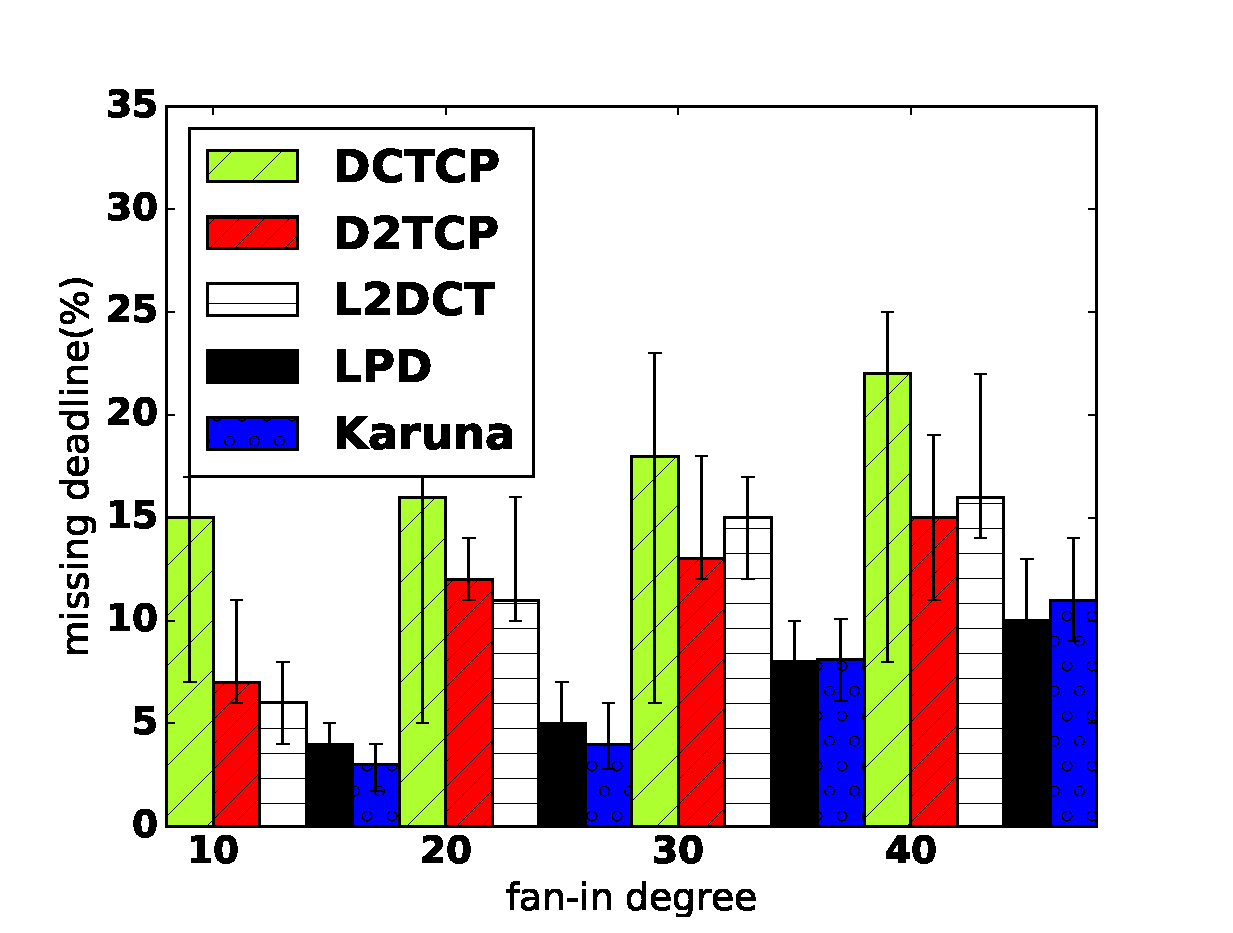
\includegraphics[width=0.32\columnwidth]{figures/LPD/old/tight.eps}}
\subcaptionbox{中等期限(30ms)}
{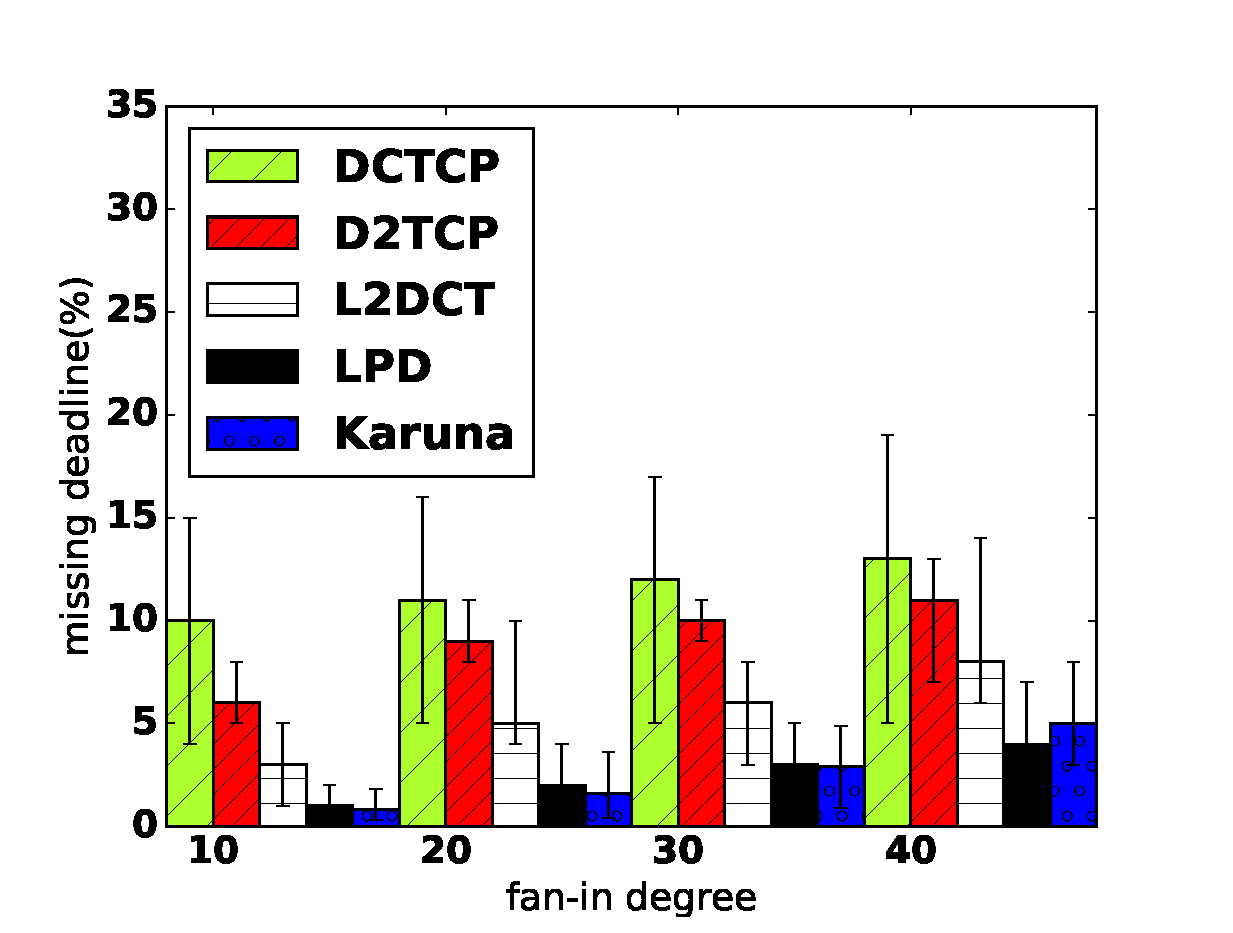
\includegraphics[width=0.32\columnwidth]{figures/LPD/old/moderate.eps}}
\subcaptionbox{松弛期限(40ms)}
{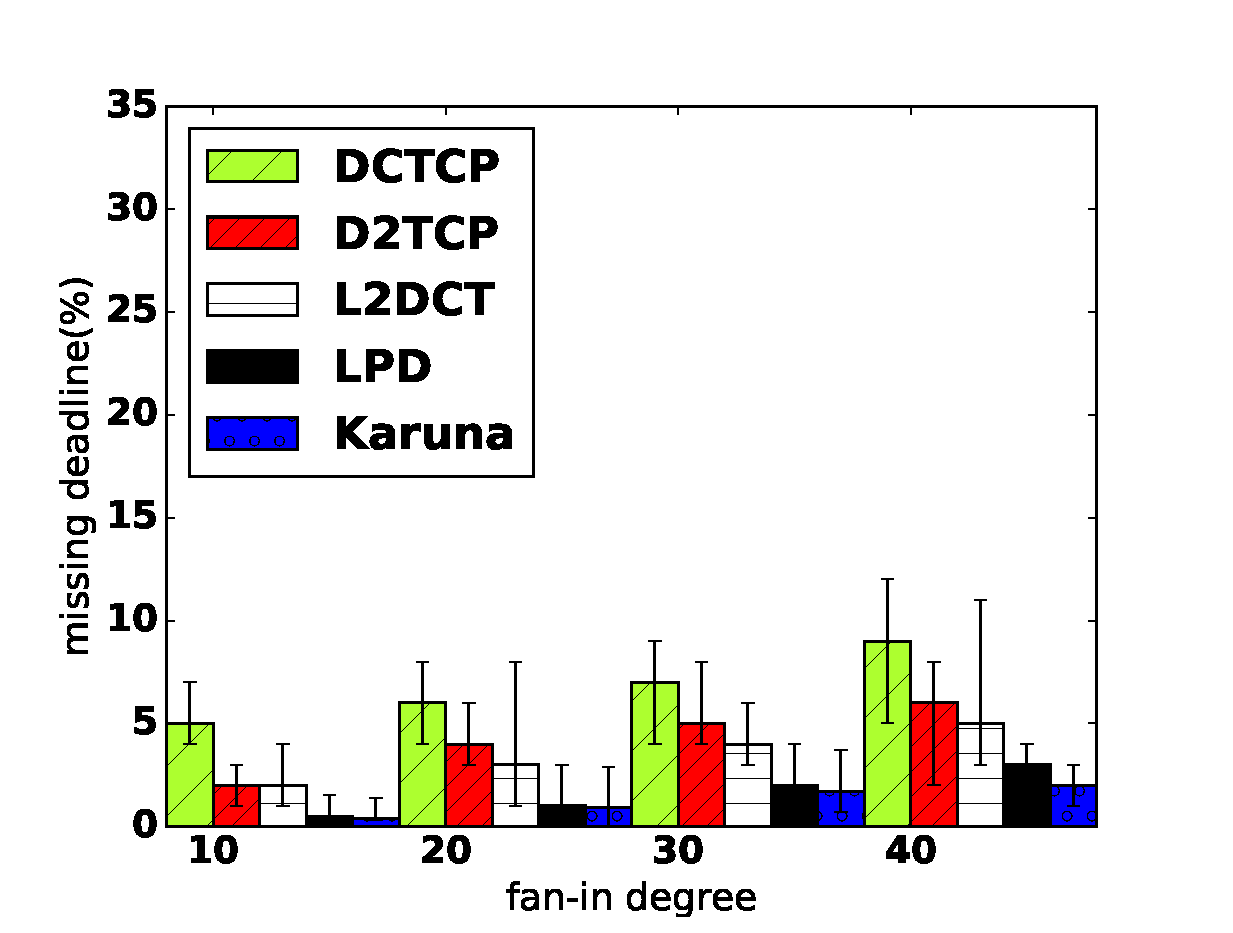
\includegraphics[width=0.32\columnwidth]{figures/LPD/old/lax.eps}}
\caption{DCTCP, D$^2$TCP, L$^2$DCT ,Karuna 和 LPD-e下OLDI应用错失期限的比例对比}
\label{Incast-dc-top-fig}
\end{figure}


\begin{figure}[h]
\centering
\subcaptionbox{紧急期限(20ms)}
 {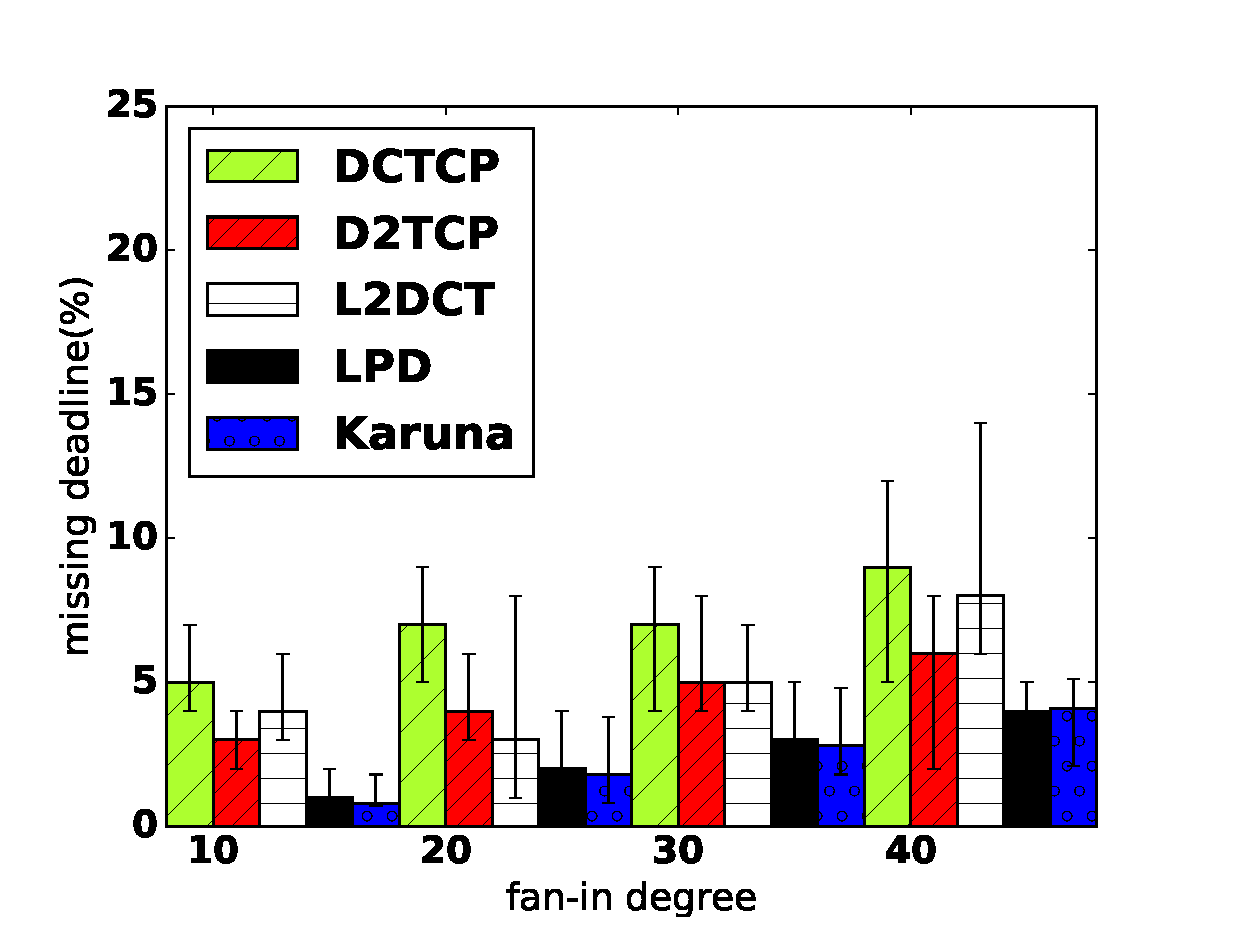
\includegraphics[width=0.32\columnwidth]{figures/LPD/old/tight1.eps}}
\subcaptionbox{中等期限(30ms)}
{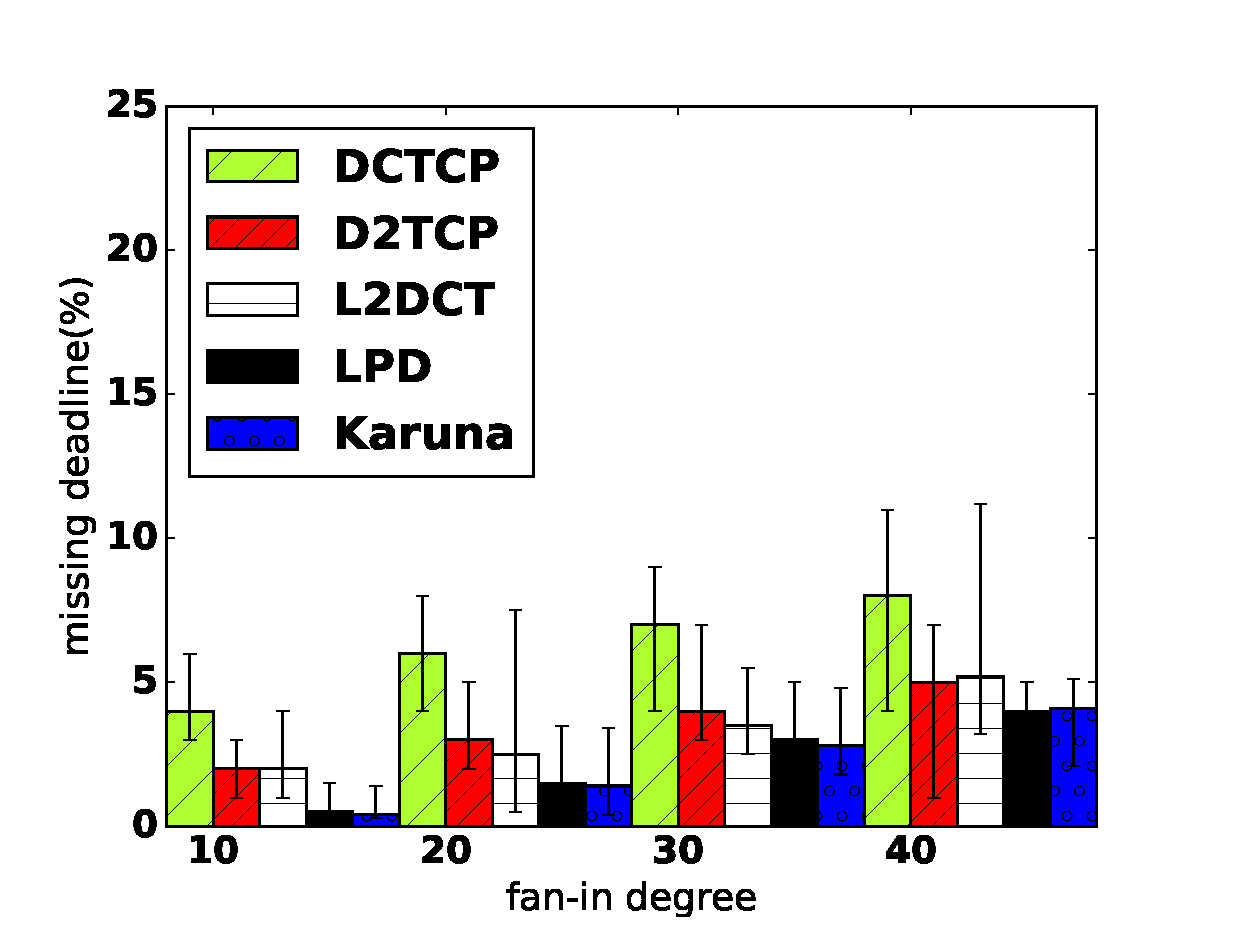
\includegraphics[width=0.32\columnwidth]{figures/LPD/old/moderate1.eps}}
\subcaptionbox{松弛期限(40ms)}
{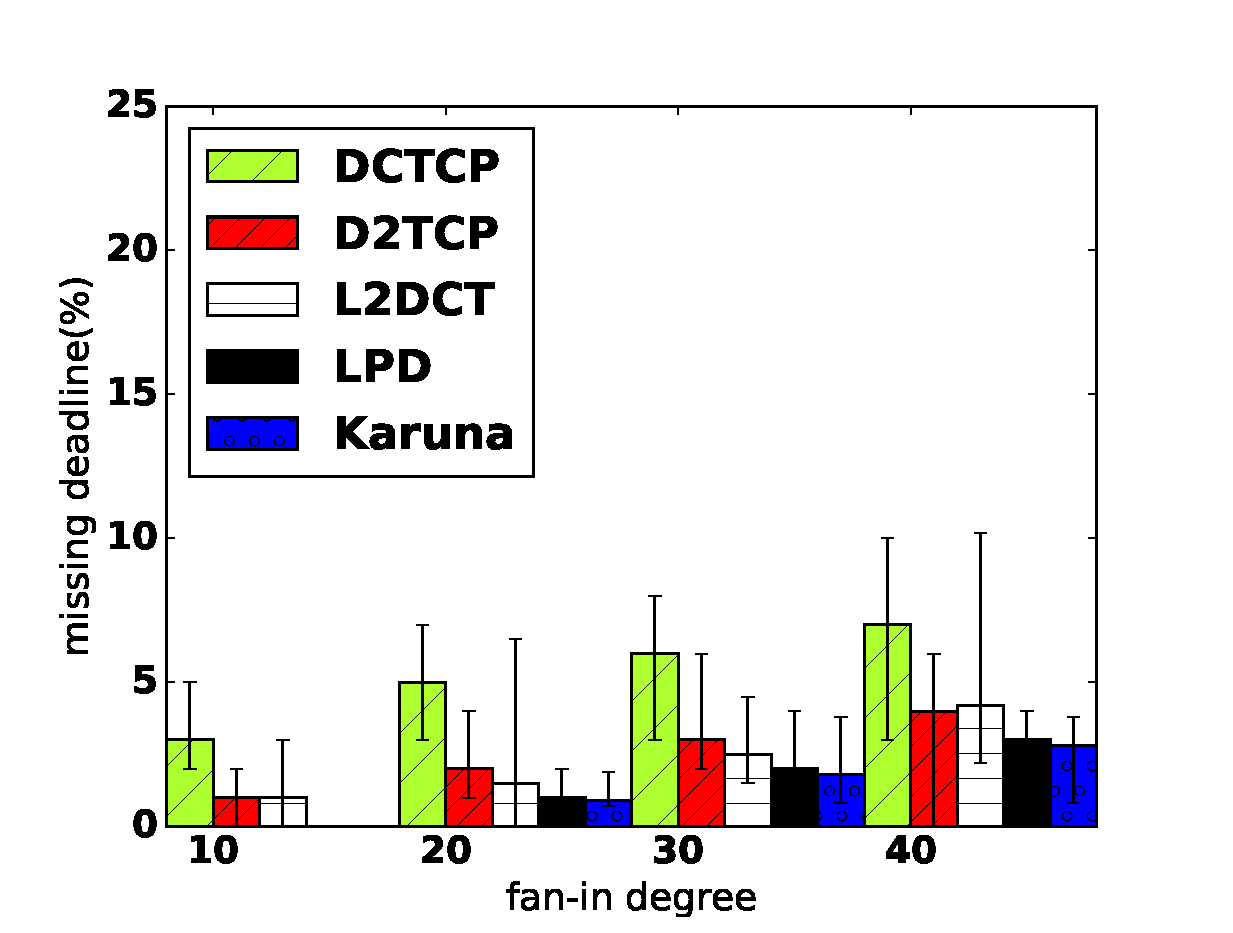
\includegraphics[width=0.32\columnwidth]{figures/LPD/old/lax1.eps}}
\caption{DCTCP, D$^2$TCP, L$^2$DCT ,Karuna 和 LPD-e,流大小分布为Pareto分布的错失期限比例}
\label{miss-dc-posson-fig}
\end{figure}

\begin{figure}[h]
\centering
\subcaptionbox{紧急期限(20ms)}
 {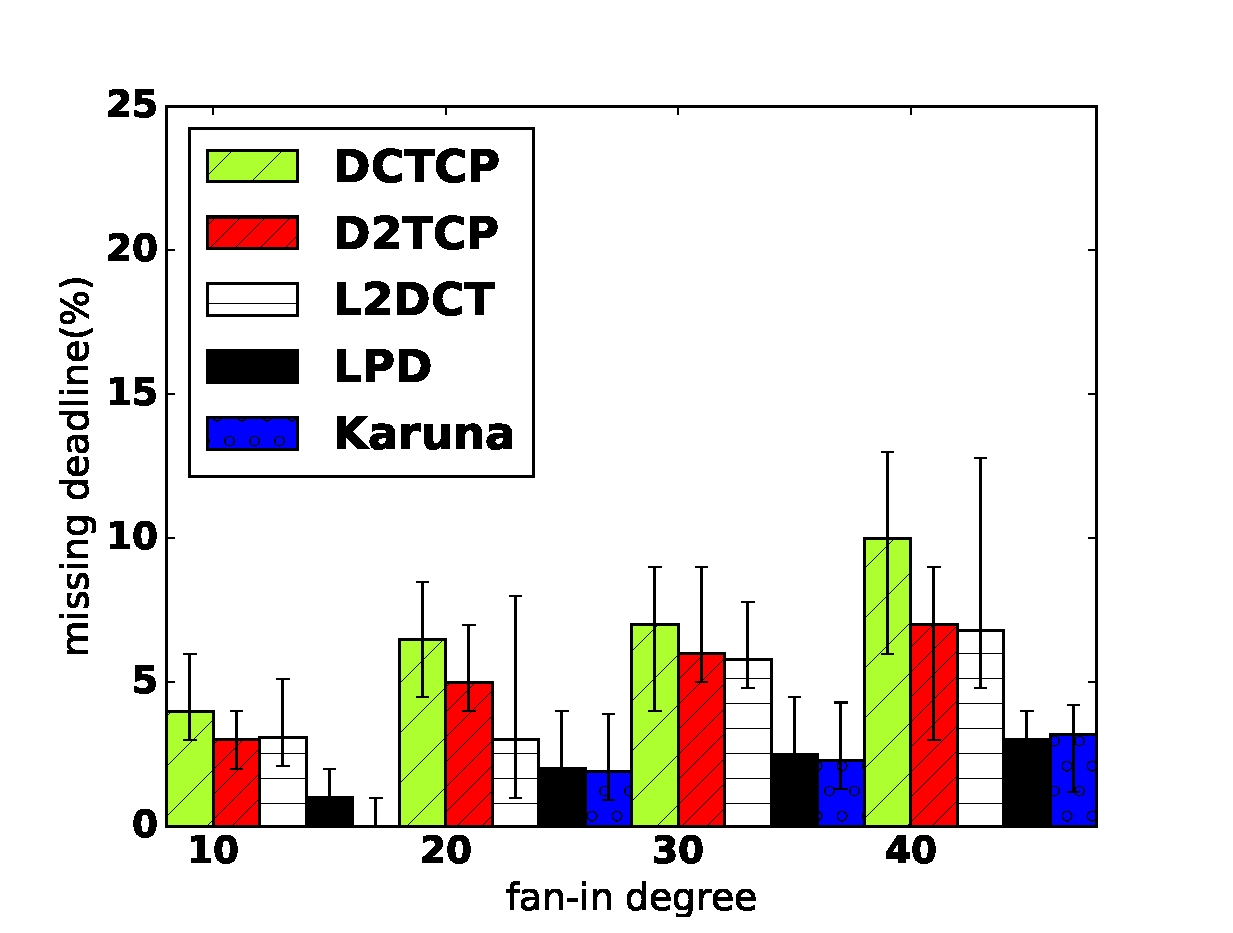
\includegraphics[width=0.32\columnwidth]{figures/LPD/old/tight2.eps}}
\subcaptionbox{中等期限(30ms)}
{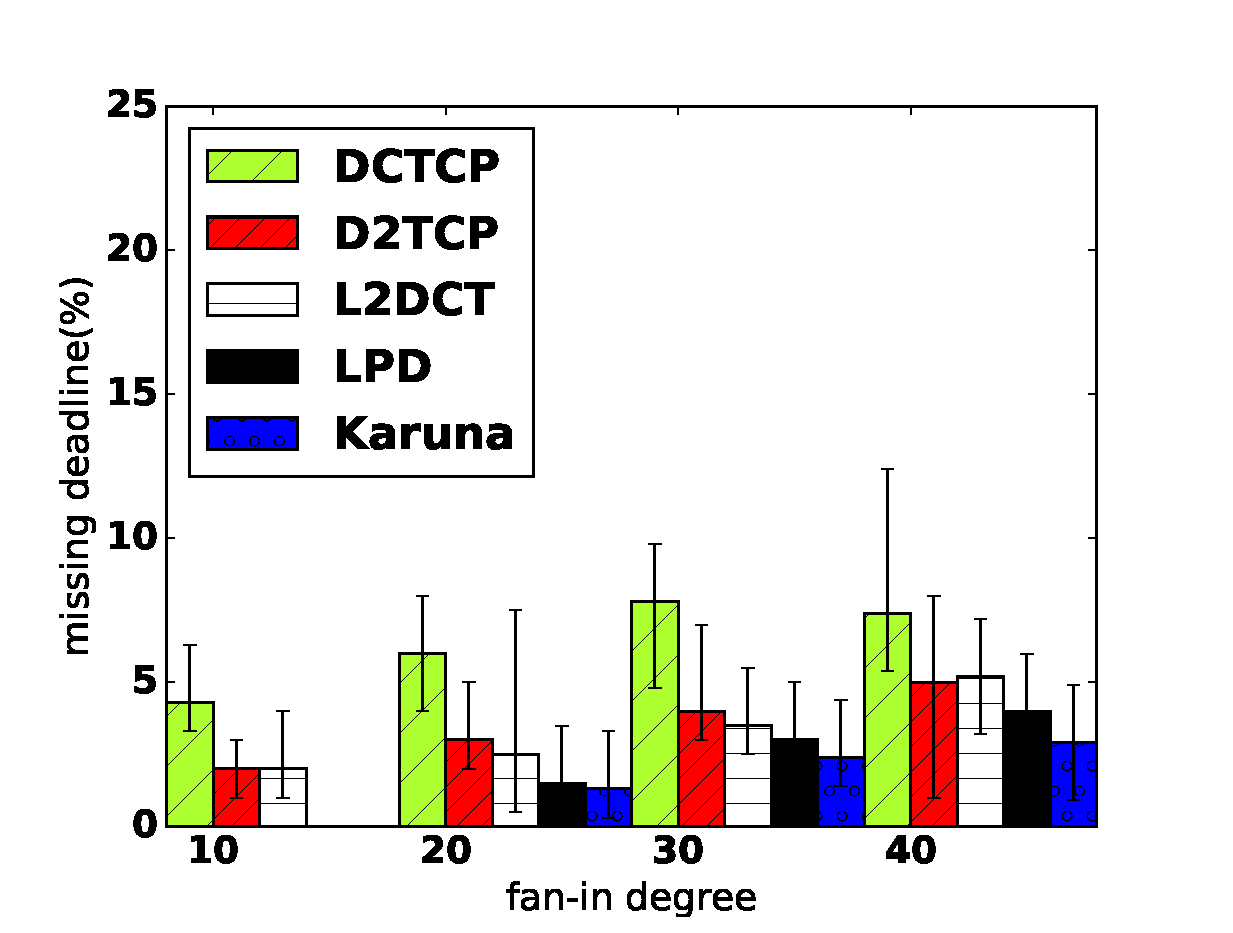
\includegraphics[width=0.32\columnwidth]{figures/LPD/old/moderate2.eps}}
\subcaptionbox{松弛期限(40ms)}
{\includegraphics[width=0.32\columnwidth]{figures/LPD/old/lax2.eps}}
\caption{DCTCP, D$^2$TCP, L$^2$DCT ,Karuna 和 LPD-e,流的期限为随机分布}
\label{miss-dc-uniform-fig}
\end{figure}


图\ref{Incast-dc-top-fig}显示了不同扇入度下流错失期限的百分比。
为了更好的展示LPD的性能,本文使用DCTCP,D$^2$TCP,L$^2$DCT,Karuna和LPD-e作为对比方案。
变换每组实验参数100次,图\ref{Incast-dc-top-fig}显示的结果中,每个柱状图显示错失期限流的百分比的平均值,
其中error bar展示了错失期限的流百分比最小值和最大值。
注意到,L$^2$DCT也是一种基于TCP的拥塞速率控制机制。
与D$^2$TCP类似,L$^2$DCT也使用gamma函数进行拥塞窗口的计算,但是和D$^2$TCP不同的是,L$^2$DCT只使用流大小作为拥塞窗口的调整因子。
实验结果表明LPD-e在网络拥塞程度很重的情形下依然可以根据流的期限进行区分,
因此,相比DCTCP,D$^2$TCP,L$^2$DCT,Karuna等,使用LPD-e使得流错失期限的数目最少。
尽管D$^2$TCP(以及L$^2$DCT)在DCTCP上有所改进,
如图\ref{Incast-dc-top-fig}(c)所示,D$^2$TCP仅仅在期限较宽松的情况下性能比DCTCP有明显的优势,
但对期限很紧的情形,如图\ref{Incast-dc-top-fig}(a)和(b)所示,D$^2$TCP并没有明显的优势。
事实上,对此问题,D$^2$TCP\cite{D2TCP}并没有进行详细讨论。
对于最先进的基于截止期限进行速率控制的方法Karuna \cite{chen2016scheduling},性能平均比LPD-e好$5\%$。
然而,对于并发程度很高的情形(如扇入度为40),此时网络处于重度拥塞,Karuna的性能比LPD差。
其原因是随着网络拥塞程度增加,使用LPD,不同期限的流获得带宽差距越来越大,
从而,数据流获得不同带宽,因而,截止期限更近的流能获取更多的带宽,从而更有可能在截止期限之前完成。



在另一种不同的场景下测试LPD-e性能,
在此场景下,服务器之间相互发送短流,变化每台机架上服务器的数目,
设置短流的到达间隔服从泊松过程(每台服务器每秒钟发送1000条数据流),
而所有其他设置(包括流量大小分布和截止期限)与上述OLDI场景中的设置相同。
图\ref{miss-dc-posson-fig}中描绘每个策略流错失期限数目的百分比。
图中柱状图每个柱呈现的结果包括平均期错过期限的流百分比,
以及进行100次随机实验得到错过期限流的数目的最小和最大值,其中我们可以看到LPD在所有情况下,性能比其他的方法要好。
特别是当负载相对较轻的情况时(即每个机架上的10台服务器发送短流,此时网络拥塞程度较轻),
无论截止期限是近还是远,使用LPD-e流错失期限的数目都是0。
与其他协议相比,除了当网络负载很重的时(即每个机架有40个服务器发送短流量时),
在几乎所有情形下,使用LPD-e,错过截止时间的流的数目降低$50\%$以上。
在负载很重时,与其它协议相比,LPD-e仍然可以将错失期限的流的比例降低至少$30\%$。

假设流大小在2 KB到200 KB范围内均匀分布,
流的期限服从平均值为30 ms,40ms和50ms的指数分布。
其它实验参数和上述其它实验相同,
实验结果结果如图\ref{miss-dc-uniform-fig}所示,不管拥塞的程度是轻微,中等还是重度,LPD-e仍然性能最好。
注意到,在所有的仿真结果中,L$^2$DCT通常可以达到与D$^2$TCP相当的结果,猜测这是由于它们都使用了伽马校正功能。
此外,在大多数情况下,Karuna表现比LPD-e更好,但是在网络负载较重的情况下,
有时LPD-e可以比Karuna表现更好,这是因为LPD-e的设计中遵循 “越拥塞,越区分”的原则,
当网络拥塞程度严重时,不同期限的数据流获得的带宽区分很大,因此更多紧急的数据流能在截止期限之前完成。

\subsubsection{复杂拓扑下测试}
\begin{figure}[H] 
  \centering
  \includegraphics[width=0.8\columnwidth]{figures/LPD/spineleaf.pdf}
  \caption{数据中心spine-leaf拓扑}
\label{DataCenterspineleaf-fig}
\end{figure}

为了展示LPD如何在复杂的数据中心拓扑结构下的性能,
以及LPD在真实流量下的性能,在ns-2模拟器中构建了spine-leaf拓扑,拓扑结构如图\ref{DataCenterspineleaf-fig}所示。
在构建的拓扑中,共有144个服务器连接到9个叶子交换机,这9个叶子交换机连接4个主干交换机。
通过主干交换机(4跳)的端到端往返延迟是14.6 us,叶交换机(2跳)的端到端往返延迟是13.3 us。
在这些延迟中,10us的时间是在端节点上,这模拟的是像hadoop这类应用的计算时间。 
TCP重传超时(RTO)设置为10 ms,初始拥塞窗口设置为12。
主干交换机和叶交换机之间的链路容量为$40 Gbps / x$,其中x为超额认购因子,叶节点和终端服务器之间的容量为10Gbps。 
K=64,设置$s_{max}$的默认值是1MB,$t_{max}$=30ms。


\begin{figure}[h]
\centering
\subcaptionbox{紧急期限(20ms)}
 {\includegraphics[width=0.32\columnwidth]{figures/LPD/spineleaf/miss_deadline_1.eps}}
\subcaptionbox{中等期限(30ms)}
{\includegraphics[width=0.32\columnwidth]{figures/LPD/spineleaf/miss_deadline_5.eps}}
\subcaptionbox{松弛期限(40ms)}
{\includegraphics[width=0.32\columnwidth]{figures/LPD/spineleaf/miss_deadline_10.eps}}
\caption{网络搜索应用流量下,LPD-e,D$^2$TCP, L$^2$DCT ,Karuna 和 DCTCP性能对比。流的截止期限是在10ms到30ms的统一分布}
\label{spine-dc-web-10}
\end{figure}



\begin{figure}[h]
\centering
\subcaptionbox{紧急期限(20ms)}
 {\includegraphics[width=0.32\columnwidth]{figures/LPD/spineleaf/miss_deadline_4.eps}}
\subcaptionbox{中等期限(30ms)}
{\includegraphics[width=0.32\columnwidth]{figures/LPD/spineleaf/miss_deadline_6.eps}}
\subcaptionbox{松弛期限(40ms)}
{\includegraphics[width=0.32\columnwidth]{figures/LPD/spineleaf/miss_deadline_9.eps}}
\caption{数据挖掘应用流量下,LPD-e,D$^2$TCP, L$^2$DCT ,Karuna 和 DCTCP性能对比。流的截止期限是在10ms到30ms的统一分布}
\label{miss-spine-data-fig}
\end{figure}


本文在实验中使用两个实际数据中心应用的流量:网络搜索(web search)和数据挖掘(data mining)\cite{DCTCP,pFabric}。
在网络搜索流中,$70\%$的流小于1 MB,超过$50\%$的流在100 KB到1 MB之间。
在数据挖掘流中,超过$80\%$数目的流是小于10KB的小流,大于1MB的长流数目约为$4\%$,长流超过$90\%$的数据量。
在本部分的仿真中,假设数据流的到达服从泊松分布。 
流的源和目标服务器是随机选择的,并且服从均匀分布。
流到达的时间间隔不同,会产生不同程度的网络负载。
当今的数据中心网络往往是超额认购\cite{CloudMirror},
在后续的实验中,本文变更超额认购参数来模拟此。






对于截止期限比较紧的流,本文选择错失期限的流的比例作为评价标准来评价算法。
对于截止期限不敏感的数据流,本文考虑流平均完成时间。
本节测试在延迟敏感的网络负载下LPD的性能。
在实际中,网络搜索等对延迟敏感的业务需要在几毫秒内将计算结果传送给客户端,否则会影响用户体验。
在下面实验中,设置截止期限在10ms到30ms之间均匀的分布。
其余的参数适用默认的值。将超额认购因子x从1改变为10,图\ref{spine-dc-web-10}显示了结果。
需要注意的是,每组实验重复100次,在图中标记处每组的平均值,最大值,最小值。



从图\ref{spine-dc-web-10}可以看出,使用LPD-e有少于1$\%$的数据流错失期限,
而使用DCTCP,D$^2$TCP,L$^2$DCT时,分别有$17\%$,$2.5\%$,$2.4\%$错失期限。
特别是,当负载和超额认购因子很小(load= 0.1,x = 1)时,D$^2$TCP和L$^2$DCT错过期限的流数目是LPD-e的2$\times$。
但是当超额因子和负载较大(load= 0.9,x = 10)时,D$^2$TCP和L$^2$DCT错过期限的流数目是LPD-e的5$\times$。
这是因为随着超额认购因子变大,网络负载变大,
LPD的惩罚函数比D$^2$TCP和L$^2$DCT的gamma校正函数性能更好,因此流错失期限的比例更小。
Karuna,当前最先进的基于期限的拥塞控制方法,有不到$1\%$的流错失期限。
然而,当网络的负载变重(负载= 0.9,x = 10)时,LPD表现比Karuna好。
这是因为,当网络负载加重时,使用LPD,不同截止期限的流的拥塞窗口差异更大。
使用数据挖掘应用的结果与之类似,结果如图\ref{miss-spine-data-fig}所示。


\begin{figure}[h]
\centering
\subcaptionbox{流平均完成时间}
 {\includegraphics[width=0.32\columnwidth]{figures/LPD/spineleaf/FCT_SEARCH_average.eps}}
\subcaptionbox{(500KB,+$\infty$)}
{\includegraphics[width=0.32\columnwidth]{figures/LPD/spineleaf/FCT_SEARCH_large.eps}}
\subcaptionbox{(0,100KB)}
{\includegraphics[width=0.32\columnwidth]{figures/LPD/spineleaf/FCT_SEARCH_small.eps}}
\caption{网络搜索流量下,LPD, L$^2$DCT ,pFabric 和 DCTCP对流平均完成时间的对比,注意图(c)和图(a),(b)的Y轴的单位不同}
\label{fct-spine-search-5-fig}
\end{figure}


\begin{figure}[h]
\centering
\subcaptionbox{流平均完成时间}
 {\includegraphics[width=0.32\columnwidth]{figures/LPD/spineleaf/FCT_DATA_average.eps}}
\subcaptionbox{(500KB,+$\infty$)}
{\includegraphics[width=0.32\columnwidth]{figures/LPD/spineleaf/FCT_DATA_large.eps}}
\subcaptionbox{(0,100KB)}
{\includegraphics[width=0.32\columnwidth]{figures/LPD/spineleaf/FCT_DATA_small.eps}}
\caption{数据挖掘流量下,LPD, L$^2$DCT ,pFabric 和 DCTCP对流平均完成时间的对比,注意图(c)和图(a),(b)的Y轴的单位不同}
\label{fct-spine-data-5-fig}
\end{figure}


\begin{figure}[h]
\centering
\subcaptionbox{流平均完成时间}
 {\includegraphics[width=0.32\columnwidth]{figures/LPD/spineleaf/average_fct.eps}}
\subcaptionbox{(500KB,+$\infty$)}
{\includegraphics[width=0.32\columnwidth]{figures/LPD/spineleaf/large_fct.eps}}
\subcaptionbox{(0,100KB)}
{\includegraphics[width=0.32\columnwidth]{figures/LPD/spineleaf/small_fct.eps}}
\caption{网络搜索流量下,LPD, L$^2$DCT ,pFabric 和 DCTCP对流平均完成时间的对比,变幻超额认购参数从5到30}
\label{fct-spine-fct-factor-fig}
\end{figure}


“越拥塞,越区分”的原则也可以用于其他目标的优化,比如流平均完成时间(Average Flow Completion Time,简称AFCT)。
改动LPD,并且设置惩罚函数为$f = s / s_{max}$,得到优化流平均完成时间的策略LPD-s。
在LPD-s中,s设置为流大小或剩余流大小。
在后续实验中,默认s设置为流大小,并设置$s_{max} = 1MB$。
对于大于1 MB的流,设置s = 1MB。
对于小于10KB的流,设置s=10KB。
假设N = 1,根据(\ref{tmax}),
LPD-s的流大小调整区域是[10KB,1MB]。
设置超额订购因子x = 5,图\ref{fct-spine-search-5-fig}显示了网络搜索应用下的流平均完成时间结果。


从图\ref{fct-spine-search-5-fig}可以看出,LPD-s和L$^2$DCT均比DCTCP的平均流完成时间都小,但性能不及pFabric。
图\ref{fct-spine-search-5-fig}(a)表明,对于网络负载较轻的场景(load<0.5),LPD-s的性能是DCTCP的3$\times$,大约是L$^2$DCT的$10\%$。
但当网络拥塞很重(load> 0.5)时,LPD-s性能分别比DCTCP和L$^2$DCT提高5$\times$和15$\%$。
图\ref{fct-spine-search-5-fig}(b)显示的是流大小大于500 KB的实验结果。
图\ref{fct-spine-search-5-fig}(c)是小流的结果,注意到图\ref{fct-spine-search-5-fig}(c)与图\ref{fct-spine-search-5-fig}(b)和(a)的y轴有不同的单位。


图\ref{fct-spine-data-5-fig}显示的是数据挖掘流量下流平均完成时间对比。
特别地,从图\ref{fct-spine-data-5-fig}(b)可以看出,LPD下流平均完成时间减小约$40\%$,
而图\ref{fct-spine-search-5-fig}(b)显示了对于长流,LPD在流平均完成时间方面性能提高1$\times$。
对于数据挖掘应用,因为大部分数据流长度大于1MB,因此在实验中,设置$s_{max }$= 1MB,
大于1MB的流被认为有最低优先级,
因而长流的优先级低。

为了测试LPD在网络负载很重的情况下的性能,我们将超额认购因子从5改变到30。
对于每组实验,将网络负载从0.1改变到0.9,图\ref{fct-spine-fct-factor-fig}显示了平均流完成时间和流完成时间的最大值以及每组的最小值。
可以观察到超额认购因子比较小(x= 5)时,LPD的平均流完成时间与L$^2$DCT相比下降了$20\%$。
但是,当网络的超额认购因子较大时,LPD的性能比L$^2$DCT提高1$\times$。
这个结果表明在网络拥塞重的情形下LPD是更优策略。


\subsection{真实环境下测试}


\begin{figure}[h]
\centering
\subcaptionbox{3条长流带宽}
 {\includegraphics[width=0.45\columnwidth]{figures/LPD/Realtest/realbandwidth2.eps}}
\subcaptionbox{队列长度}
{\includegraphics[width=0.45\columnwidth]{figures/LPD/Realtest/realqueue2.eps}}
\caption{流区分}
\label{real-fig}
\end{figure}


\subsubsection{简单拓扑下的测试}
为了在真实环境下测试LPD的性能,在Linux内核3.2.61中基于DCTCP的代码实现了D$^2$TCP和LPD-e。
交换机使用NetFPGA来实现,并且每个交换机都有4个1Gbps以太网端口,因此数据包可以线速转发和标记。
由于硬件有限,我们只能建立两台交换机和六台服务器的小数据中心拓扑结构。
LPD对Linux内核3.2.61评估的主要代码可以在\cite{LPD-code}下载。


本文首先验证LPD-e是否可以在真实环境中区分不同期限的流量,
流大小设置为10,30和50 MB,相应的截止时间为300,600和900 ms。
图\ref{real-fig}绘制了每个流的带宽随时间的变化情形,以及交换机上的队列长度。
与仿真结果类似,不同截止期限的流程明显不同,队列长度保持在37.5 KB的标记阈值(约为K = 25个1.5 KB的数据包)。

\begin{figure}[H] 
  \centering
  \includegraphics[width=0.5\columnwidth]{figures/LPD/realtopology.pdf}
  \caption{小型数据中心测试床}
\label{testbed-fig}
\end{figure}


\begin{figure}[h]
\centering
\subcaptionbox{随机目的}
 {\includegraphics[width=0.45\columnwidth]{figures/LPD/Realtest/miss_deadline_1.eps}}
\subcaptionbox{OLDI}
{\includegraphics[width=0.45\columnwidth]{figures/LPD/Realtest/miss_deadline_2.eps}}
\caption{LPD 和 DCTCP, D$^2$TCP错失期限对比}
\label{testbed-deadlinemiss-fig}
\end{figure}




\begin{figure}[h]
\centering
\subcaptionbox{随机目的}
 {\includegraphics[width=0.45\columnwidth]{figures/LPD/Realtest/fct_1.eps}}
\subcaptionbox{OLDI}
{\includegraphics[width=0.45\columnwidth]{figures/LPD/Realtest/fct_2.eps}}
\caption{LPD 和 DCTCP,L$^2$DCT流完成时间对比}
\label{testbed-fct-fig}
\end{figure}

\begin{figure}[h]
\centering
\subcaptionbox{OLDI}
 {\includegraphics[width=0.45\columnwidth]{figures/LPD/evaluation_3/lpd.eps}}
\subcaptionbox{网络搜索流量}
{\includegraphics[width=0.45\columnwidth]{figures/LPD/discussion/diss_miss_deadline_.eps}}
\caption{设计原则的进一步拓展}
\label{discussion-fig}
\end{figure}


\begin{figure}[h]
\centering
\subcaptionbox{紧急期限 (20ms)}
 {\includegraphics[width=0.32\columnwidth]{figures/LPD/discussion/20ms.eps}}
\subcaptionbox{中等期限 (30ms)}
{\includegraphics[width=0.32\columnwidth]{figures/LPD/discussion/30ms.eps}}
\subcaptionbox{松弛期限(40ms)}
{\includegraphics[width=0.32\columnwidth]{figures/LPD/discussion/40ms.eps}}
\caption{LPD-r和LPD-e下,OLDI应用期限错失对比}
\label{discussion-r-fig}
\end{figure}


\begin{figure}[h]
\centering
\subcaptionbox{网络搜索流量}
 {\includegraphics[width=0.45\columnwidth]{figures/LPD/discussion/web_search.eps}}
\subcaptionbox{数据挖掘流量}
{\includegraphics[width=0.45\columnwidth]{figures/LPD/discussion/data_mining.eps}}
\caption{LPD-r和LPD-e的下的网络搜索和数据挖掘流量下错失期限对比,流截止期限在10ms到30ms之间,超额认购因子为10}
\label{discussion-r2-fig}
\end{figure}



\subsubsection{小型数据中心测试}
建立一个小型的基于树的测试环境来测试LPD的性能。
图\ref{testbed-fig}显示了拓扑结构。
在此拓扑结构下,两台Linux服务器运行Ubuntu14.04以及dummynet \cite{dummynet,MPTCP} 来构建一个双向瓶颈链路。
修补dummynet用来标记数据包。
在实验中,拓扑中所有接口都是1Gbps。


LPD的惩罚函数遵循“越拥塞,越区分”的原则,即使在网络重度拥塞的的条件下也能区分期限不同的数据流。
因此更多的流能够在最后截止期限前完成。
在实验中,每个服务器$S_i$随机与服务器$S_j$(i$\neq$j)建立连接。
随后$S_i$连续发送数据流给$S_j$。
然后记录数据流错失期限的平均值,最大值和最小值。
图\ref{testbed-deadlinemiss-fig}(a)显示的结果。
可以看到LPD比D$^2$TCP和DCTCP更好。
与DCTCP和D$^2$TCP相比,LPD下流错失期限的比例减少了约$50\%$和$30\%$。
为了观察在OLDI应用下LPD的性能,让$S_1\sim S_6$连续向根R节点发送随机截止期限($\le$10ms)的小流,
图\ref{testbed-deadlinemiss-fig}(b)显示了结果。
可以观察到,LPD比DCTCP性能提高约$30\%$,比D$^2$TCP提高大约$20\%$。
为了测试LPD在减少流完成时间方面的性能,让每个服务器$S_i$将流发送到随机目的节点,
流发送过程持续2分钟,重复这个过程20次,图\ref{testbed-fct-fig}(a)显示了实验结果。
可以看到,与DCTCP和L$^2$DCT相比,LPD流平均完成时间减少了约$20\%$和$10\%$。
随后测试LPD在Partitions-Aggregate的性能,
首先让根节点服务器R向每个端节点发送查询请求,
在端节点接收到查询请求后,它将发送流大小为K的响应数据流。
将K从50 KB变为200 KB,图\ref{testbed-fct-fig}(b)显示实验结果。
可以看到,与DCTCP和L$^2$DCT相比,LPD-s使流平均完成时间分别减少$20\%$和$10\%$。
这是因为LPD采用具有“越拥塞,越区分”的惩罚函数,因此端节点的拥塞控制机制在负载很重的情形下依然有效。

\section{对“越拥塞,越区分”原则的讨论}
 “越拥塞,越区分”这个原则是具有通用性的,本文的策略使用的控制形式:
\begin{equation}
w=
\begin{cases}
w+(1-f) &\text{没有拥塞;}\\
w \times (1-f) &\text{发生拥塞}
\end{cases}\nonumber
\end{equation}
本部分,使用不同的惩罚函数来测试“越拥塞,越区分”原则的通用性。
\subsection{不同的惩罚函数}
设f=a/d,其中d是在D$^2$TCP中使用的期限因子,使用f=a/d作为惩罚函数,
把这个策略成为LPD-d。
LPD-d已经用来解决研究动机提出的问题。
此外,引入另一种拥塞控制机制:
$$ f=\left\{
\begin{array}{rcl}
(2-d)^\alpha      &      & {0      <d      <1}\\
\alpha    &      & {d=1}\\
\alpha*\frac{2-d}{2d-\alpha}     &      & {d>1}\\
\end{array} \right. $$
可以证明$\frac{\partial{(1-f)}}{\partial{d}}>0$, 此外$\frac{\partial^{2}{(1-f)}}{\partial{\alpha}\partial{d}}>0$,
此例符合本文提出的“越拥塞,越区分”的原则,称之为MLD。


设置流的期限满足统一分布,图\ref{discussion-fig}(a) 描述了OLDI应用下LPD-e, MLD 和 LPD-d性能对比。
图\ref{discussion-fig}(b)下网络搜索流量下的结果。
图\ref{discussion-fig}显示不同形式的算法的差异性不大,
策略能够在网络拥塞程度重的情形下使的期限不同的数据流。

\subsection{使用其他属性}

在\ref{sec_LPD:LPD}节中提出LPD-e,使用流程开始时间和截止期限之间的时间间隔。
因为,减少流错失期限的最优策略是最小期限优先策略。 
使用另一种策略,使用当前时间和截止期限之间的持续时间作为调整因子,称之为LPD-r策略。
 
 
使用的相同参数来评估LPD-r,并将其与LPD-e进行比较。
 图\ref{discussion-r-fig}描绘了在简单拓扑下OLDI应用LPD-r与LPD-e错失期限情形对比。
 而图\ref{discussion-r2-fig}描绘了在spine-leaf拓扑中的在网络搜索和数据挖掘下错失期限对比。
从实验结果中,可以看到LPD-r和LPD-e性能相近,
这再一次证实了“越拥塞,越区分”原理的通用性,
因此在实际中,可以使用不同的惩罚函数以及不同的期限因子设计拥塞控制机制。

\section{本章总结}
\label{sec_LPD:Conclusion}
本章提出“越拥塞,越区分”的原则来设计数据中心拥塞控制机制。
根据本原则设计的拥塞控制机制,使的网络即使在严重拥塞的情形下依然可以根据截止期限分配带宽。
为了证明这个原则的有效性,本文设计了速率控制机制-负载自适应拥塞控制策略(load proportional differentiation,简称LPD),
并使用不同的网络拓扑和网络流量测试LPD的性能。
实验发现LPD的性能几乎超越了例如D$^{2}$TCP, L$^{2}$DCT等当前最先进的拥塞控制机制。

尽管LPD用来使的更多数据流在截止期限之前完成,原则“越拥塞,越区分”是有通用性,
用户可以根据这个原则设计其它的拥塞控制机制。
然而,关于LPD的收敛性和稳定性,在以后的工作中需要进行进一步的讨论。



\chapter{基于流持续时间的传输优化方案}
\label{chapter:FDRC}
当前,许多应用(如网络搜索和零售)部署在数据中心。
由于TCP不能满足应用对延迟和吞吐量的需求,
因此研究者们提出了许多传输协议(例如,DCTCP,D$^2$TCP,L$^2$DCT)来对TCP进行补充。
其中,D$^2$TCP等协议将流的截止期限纳入拥塞窗口调整过程,以保证流在截止期限之前传输完成。
在数据中心中,短流常常需要较短延迟,因而,L$^2$DCT等协议在计算拥塞窗口调整因子时考虑流大小,以此保证短流的吞吐量和延迟。
这两种方法在一定的场景下运行良好,但依旧存在一些不足:
首先,这两种方法只能减小流错失期限的百分比或者能够减小流平均完成时间,但是不能够同时优化这两个目标。
其次,大多数方法都需要预知流的信息(例如截止期限,流大小),
但是对于很多应用,流大小以及流截止期限这些信息很难预先得知。
因此,在本章中,本文主张使引入流持续时间到拥塞窗口调整的过程中。
基于此,本文提出流持续时间速率控制机制(Flow Duration Time Rate Control,简称FDRC)。
本文发现,在不用预先得知流信息的情形下,FDRC可以减少流错失期限的比例并且能够减小流平均完成时间。
本章从理论上分析了FDRC的行为,并在ns-2和Iinux内核实现FDRC。
同时实验表明,在几乎所有场景下,FDRC比D$^2$TCP和L$^2$DCT的性能都要好。
平均来说,FDRC比基于期限的拥塞控制协议D$^2$TCP性能高30%,
比优化流平均完成时间的方法L$^2$DCT性能提高大约10% 。

\section{概述}
\label{FDRC:introduction}
如今,越来越多对延迟敏感的应用(例如网络搜索,零售)被部署在数据中心网络。
数据中心网络(DCNs)需要给应用提供高吞吐,低延迟的服务,此外还需要能够承受高并发等特殊需求。
最近,在这些需求中,延迟引起了更多的关注,因为这会影响用户在这些应用中的体验,从而影响收入。
事实上,对于数据中心应用,每增加100ms,可能导致$1\%$的收入损失\cite{DCTCP,LPD}。


特别的,数据中心的流是由长的背景流,对时延敏感的流和带宽敏感流的混合,使用TCP不能满足所有流的需求,
会导致下面的两个问题。
首先,使用TCP协议,会导致交换机缓冲区溢出,数据包重传,进而使的网络延迟加大,从而影响用户体验。
其次,网络发生拥塞时,TCP发送端拥塞窗口会减半,导致网络震荡严重,链接利用率低。
由于存在TCP以上不足,DCTCP\cite{DCTCP}被提出。 
DCTCP采用大多数现代交换机支持的ECN标记机制\cite{DCTCP},
首先在交换机上设置一个阈值K,当交换机缓冲区队列超过K时,发送到交换机的数据包会标记CE,
接收端收到所有的数据包后,如果有被标记CE的数据包,那么回复给发送端的ACK就会被标记ECN。
最后发送端统计上一个RTT中收到的ACK被标记的ECN的比例,然后计算链路拥塞程度,最后根据拥塞程度调整拥塞窗口。
DCTCP通过使的交换机缓冲区队列维持在较短水平上,从而可以减小排队延迟,同时可以维持高链路利用率。
但是,DCTCP不考虑流的期限问题,它对所有流都公平对待,这样会导致许多对延迟敏感的流错过期限\cite{D2TCP,D3}。
针对此,业界提出两类方法来弥补TCP的不足:

\textbf{(1)给流设置显式的期限。} 
例如D$^3$\cite{D3},D$^2$TCP\cite{D2TCP}和LPD\cite{LPD}这几个方法是
从用户态给应用的数据流设置期限,数据流带宽由网络拥塞程度和期限共同决定。
截止期限近的数据流得到的带宽比期限远的流得到的带宽多,
因此,截止期限近的流和截止期限远的流都能在截止时间之前完成。
通过设置不同的截止期限,优化数据流的传输延迟。

\textbf{(2)将短流设置为高优先级。}
在数据中心网络中,短流常常承载交互等信息,因此往往需要低延迟。
所以PDQ \cite{PDQ},L$^2$DCT\cite{L2DCT}和pFabric \cite{pFabric}等试图将短流设置为高优先级,长流设置为低优先级,
并试图实现最短流优先策略(Shortest Job First,简称SJF)。
事实上,在单条瓶颈链路的场景下,
最短流优先策略是减小流平均完成时间的最优策略。
事实上,在多链路的情形下,
最短流优先策略也能达到较好的性能\cite{L2DCT,pFabric}。


事实上,这两种方法都试图把紧急的流设置更高的优先级,优化紧急流的延迟。
区别在于第一种方法是根据用户期望的延迟设置优先级,第二种是根据流的大小设置优先级。
两种方法都需要用户事先得知流信息。
具体的,如果使用第一类方法,需要事先得知流的截止时间;如果使用第二类方法,需要事先得知流大小。
另外,数据中心的流是延迟敏感流,带宽敏感流和长的背景流的混合,
第一类方法可以满足延迟敏感流的需求,第二类方法只是试图降低流的平均完成时间。
事实上,这两种方法都不能同时满足延迟敏感流,带宽敏感流和长的背景流的需求,
所以这些方法在部署上有一定的局限性。

由于以上提到的缺陷,本文提出流的优先级可以根据流启动的持续时间来设置。
流在开始发送时具有最高优先级,随着时间的推移其优先级下降。
 一方面不需要事先知道流的信息(流的大小或截止时间);
另一方面,这种方法间接给短流设置了更高的优先级,短流经常有期限限制,短流能获得较多的带宽,
进而能够在截止时间之前完成,同时优化了流的平均完成时间。
基于此,本章提出了基于流持续时间的速率控制算法(Flow Duration Rate Control,简称FDRC)。
本章将FDRC实现在ns-2\cite{ns2}和Iinux 内核3.2.61上。
实验结果表明FDRC的性能比D$^2$TCP提高了$30\%$,比DCTCP提高了2$\times$。
本章中主要做了以下的工作:

(1)提出数据中心基于流持续时间的传输协议(Flow Duration Rate Control,简称FDRC)。
FDRC可以使更多流达到最终期限的限制,同时有助于减少流平均完成时间。
FDRC可以在事先不知道流信息的情形下,有效的减少流错过期限数目的百分比。

(2)在ns-2中评估FDRC,然后用DCTCP,D$^2$TCP,L$^2$DCT,LPD和pFabric与之对比。
最后,在linux内核中实现FDRC,并构建小型数据中心测试FDRC,进而评估FDRC的性能。


\section{相关工作和研究动机}
\label{FDRC:background}
\subsection{相关工作}

业界已经提出一系列方法来保证数据中心流传输延迟,
根据这些方法特性可以分为三类,第一类是基于TCP的方法,例如
DCTCP\cite{DCTCP},D$^2$TCP\cite{D2TCP}以及LPD\cite{LPD}等,
这类方法一般借助交换机ECN标记机制,通过ECN机制来评估交换机队列长度,
根据网络拥塞程度和流特性(期限,流大小)等进行速率控制;
第二类是网络调度方法,例如PDQ\cite{PDQ},D$^3$\cite{D3}等,
这类方法通常采用集中控制的方法,在此系统中,有一个集中控制器,
集中控制器需要预先得知网络的情形,根据网络实时拥塞状况对流进行调度;
第三类是控制交换机队列的方法,例如pFabric\cite{pFabric}等,
这类方法需要改动交换机队列,在交换机上实现特殊的队列控制机制,通过特殊队列进出方式,实现对流的速率控制。


以上的三类方法,无论是显式设置期限还是隐式的优化流完成时间,
都需要预知流的信息(流大小,截止期限,剩余流大小,剩余时间等)或者对网络设备进行修改。
但是在数据中心的流是混合了延迟敏感流,带宽敏感流和长的背景流。
给流设置截止期限,根据截止期限区分优先级,能够减少流错失期限的比例。
根据流大小进行调整,只能够优化流完成时间。
但是当前没有一种方法能够同时满足这两者的需求,此外这些方法还需要预先得知流信息。
实际需要一种无须知道流的信息就能够优化有截止期限的流和流完成时间。

\subsection{研究动机}\label{fdrc_motivation}

\begin{figure}[h]
\centering
\subcaptionbox{错失期限流比例}
 {\includegraphics[width=0.32\columnwidth]{figures/FDRC/motivation/miss_deadline.eps}}
\subcaptionbox{流平均完成时间}
{\includegraphics[width=0.32\columnwidth]{figures/FDRC/motivation/fct.eps}}
\subcaptionbox{背景流带宽}
{\includegraphics[width=0.32\columnwidth]{figures/FDRC/motivation/bandwidth.eps}}
\caption{研究动机: $50\%$的流有显式的期限,其他的流应该尽快的传输完}
\label{fdrc-motivation-fig}
\end{figure}

当前速率控制算法,无论是设定显式截止期限或者给短流设置高优先级,优化流平均完成时间,
可以使流在截止期限之前完成或减少流平均完成时间,但是不能同时满足两个目标。
为了验证此问题,在ns-2平台上,启动10个发送端,1个接收端,
它们共同连接到一个交换机上,设置交换机的缓冲区的阈值K$=25$。
实验中的所有链路均设置1Gbps的带宽,
在10个发送端中,有2个持续发送背景流,
另外8个不断发送大小从100KB到1MB的短流,将短流量平均分为两组:
对于第一组(4个发送端),期望短流能够在$30ms$之内完成传输(截止期限为30ms);
对于第二组(4个发送端),期望流平均完成时间尽可能短。
仿真时间持续10分钟,最终结果如图\ref{fdrc-motivation-fig}所示。

图\ref{fdrc-motivation-fig}(a)显示了几种方案下错失期限的流数目对比,
图\ref{fdrc-motivation-fig}(b)显示了流平均完成时间的对比。
图\ref{fdrc-motivation-fig}(a)所示,D$^2$TCP比L$^2$DCT 和DCTCP性能更好,
图\ref{fdrc-motivation-fig}(b)所示,对于流平均完成时间,L$^2$DCT性能更好。
这是因为使用D$^2$TCP,有显式期限的紧急流优先级较高,
从而获得较多的带宽,因而更有希望在截止时间之前完成。
但是,使用DCTCP和L$^2$DCT,第一组有期限的流与背景流的优先级相同,
因此很多期限近的流无法获得更多的带宽,从而会错失截止期限。
对于流平均完成时间,L$^2$DCT比D$^2$TCP性能更好,
这是因为在L$^2$DCT中,短流优先级高于长流,优先完成短流,
因此能够优化流平均完成时间,但是在实际中并不是所有的短流都有期限,
因而,对于有期限的流,L$^2$DCT并不能完全优化,所以,很多有期限的流并不能在截止时间之前完成。
图\ref{fdrc-motivation-fig}(c)显示了背景流的带宽。
可以看到,DCTCP下的背景流的带宽比D$^2$TCP与L$^2$DCT下背景流带宽高。


从图\ref{fdrc-motivation-fig}可以得出以下结论:
D$^2$TCP可以减少流错失期限的比例,L$^2$DCT 可以减少流平均完成时间。
但是,无论D$^2$TCP还是L$^2$DCT均不能同时满足这两个目标。
这是因为D$^2$TCP使用截止期限(deadline)作为速率控制因子,所以截止期限近的流将比截止期限远的流有更大的带宽。
但是D$^2$TCP无法优化流平均完成时间。
L$^2$DCT 使用流大小作为速率控制因子,因此小流将比长流有更高的平均带宽。
但是,在数据中心,并不是所有短流都有明确的截止期限(deadline),有些流只需要尽可能快的传输(例如小的请求)。
L$^2$DCT 将导致流平均完成时间较短,但是对于有显式期限的数据流会错失期限。

由于数据中心的流是有紧急期限的流,带宽敏感的流(希望流完成时间短)的混合,
所以需要一个协议来同时满足这两种流的需求。
当前无论D$^2$TCP或者L$^2$DCT均不能达到此目的,
它们只能优化有期限的流或者优化流完成时间,而无法同时满足两种需求。
因此,建议把流持续时间作为速率调整因子引入到流的速率控制中。
开始启动时,流具有最高优先级,随着时间流逝,流优先级下降。
引入流持续时间是一个很好的选择,
因为一方面这会使短流具有较高的平均带宽,
所以流有较短的平均完成时间;
另一方面,在固定时间阈值内的流将具有较大的平均带宽,
对于有期限的流也是一种较好的优化方法。


\section{FDRC策略}

\subsection{基于流持续时间的速率控制策略}

\begin{algorithm}
\KwIn{流启动时刻 $time\_start$,当前时刻  $time\_now$ }
\KwOut{窗口调整因子 $d$}
 $durtime=time\_now-time\_start$\;
  \If{durtime $\le threshold\_tight$}{
              $d=DMIN$\;
   }\ElseIf{durtime $\ge threshold\_lax$}{
   	  $d=DMAX$\;
   }\Else{
   d=$DMIN+\frac{(durtime-threshold\_tight)*(DMAX-DMIN)}{threshold\_lax-threshold\_tight}$
   }
   \textbf{return} d;
\caption{拥塞窗口因子计算算法}
\label{factor_algorithm}
\end{algorithm}

将流持续时间引入拥塞窗口控制,基于此,本文提出了基于流持续时间的策略(Flow Duration Rate Control,简称FDRC)。
算法\ref{factor_algorithm}展示了计算期限因子的步骤。
算法\ref{factor_algorithm}计算期限因子,需要四个参数: 
$threshold\_tight$和$threshold\_lax$是时间阈值,$DMAX$和$DMIN$是期限因子的上限和下限,当流的持续时间大于$threshold\_lax$时,
期限因子d被设置为$DMIN$,当流持续时间小于$threshold\_tight$,期限因子$d$被设置为$DMAX$。
当持续时间短于$threshold\_tight$时,流保持最高优先级。
如果流持续时间大于$threshold\_lax$,则流保持最低优先级。
对于$threshold\_tight$和$threshold\_lax$之间的流,优先级随着时间的推移而下降。
算法\ref{factor_algorithm}在每个RTT执行一次。
随着时间的推移,流优先级下降,因此,长的背景流的带宽平均值小于短流的带宽,流完成时间长。

\subsection{FDRC 协议}
FDRC基于DCTCP,在交换机端使用ECN标记模式。
交换机预先设置一个标记的阈值$K$。
当队列长度大于交换机的阈值$K$时,到达的数据包将被标记CE。
然后,接收端将检查来的数据包是否被标记,
如果发送过来的数据包有CE标记,则接收端回复的ACK中有ECN标记;
如果没有CE标记,那么接收端收到的ACK中没有ECN标志。
发送方每个RTT时间段,计算一下所有ACK中被标记ECN的比例,得到拥塞程度$\alpha$:
\begin{equation}
\label{alpha}
\alpha=(1-g) \times \alpha+g\times F
\end{equation}

其中,F是上一个RTT被标记ECN的比例。g是滑动平均的因子,拥塞程度$\alpha$反应的是这一段时间内的拥塞情况。
 根据计算的拥塞程度$\alpha$,得到FDRC拥塞窗口计算方法:
\begin{equation}
\label{factor}
f=\alpha \times d
\end{equation}

根据\cite{LPD},拥塞窗口的变化的加法增加部分和乘法减少部分可以是相同的。
根据此,改动滑动窗口的变化如下:
\begin{equation}
\label{ca}
 p=\left\{
\begin{array}{rcl}
w+(1-f)\\
w*(1-f) \\
\end{array} \right. 
\end{equation}


\subsection{FDRC 分析}
在本部分,从理论上分析FDRC的性能,建立两个模型来分析FDRC的性能:锯齿模型和FDRC-fluid模型。
锯齿模型是一个粗粒度的模型,FDRC-fluid模型是细粒度的模型。
本文使用锯齿模型用来分析FDRC速率和参数的关系,使用流模型,分析FDRC的参数。

\subsubsection{FDRC锯齿模型}
本部分建立锯齿模型\cite{LPD} 来分析FDRC的带宽。
$R_{1}$ 和 $R_{2}$ 表示 $flow_1$ 和 $flow_2$的速率。
假设两条流的拥塞窗口从$w_{min}$ 增加到 $w_{max}$,
有 $w^{av}=\frac{w_{min}+w_{max}}{2}$,其中$w^{av}$表示的是平均窗口大小。
流的拥塞窗口变化是有固定周期的锯齿,滑动窗口从$w_{min}$变化到$w_{max}$,需要N个RTT。
根据(\ref{ca}),滑动窗口每个RTT增加$(1-f)$,
因此得到最大的滑动窗口和最小滑动窗口的关系:$w_{max}=w_{min}+N \times(1-f)$。
当出现拥塞时候,窗口减小到$w_{min}$,
根据(\ref{ca}),有$w_{min}=w_{max}*(1-f)$。
令$w_{1}$是flow$_1$的最大窗口,
$w_{2}$是flow$_2$的最大窗口。
根据平均滑动窗口,计算两条流的平均发送速率比:
\begin{eqnarray}\label{fdrc-rate-ratio}
\frac{R_{1}}{R_{2}} =\frac{w^{av}_1}{w^{av}_2}
\end{eqnarray}
而 $w^{av}=\frac{w_{min}+w_{max}}{2}$,$w_{max}=w_{min}+N \times(1-f)$,带入(\ref{fdrc-rate-ratio}),得到二者的速率比:
\begin{eqnarray}\label{fdrc-rate-ratio2}
\frac{R_{1}}{R_{2}} &=&\frac{(2-f_1)\times w_1}{(2-f_2)\times w_2}  \nonumber \\
&=& \frac{2-\alpha d_1}{2-\alpha d_2}\times \frac{1-\alpha d_1}{1-
\alpha d_2}\times \frac{d_2}{d_1}\nonumber
\end{eqnarray}
当 $d_1$ 和 $d_2$ 很小,有$ \frac{2-\alpha d_1}{2-\alpha d_2}\simeq 1$,$ \frac{1-\alpha d_1}{1-
\alpha d_2}\simeq 1$,因此,可以得到:
\begin{equation}
\label{Ratio}
\frac{R_1}{R_2} \simeq \frac{d_2}{d_1}
\end{equation}

\begin{figure}[h]
\centering
\subcaptionbox{滑动窗口}
 {\includegraphics[width=0.48\columnwidth]{figures/FDRC/model/rate.eps}}
\subcaptionbox{队列长度}
{\includegraphics[width=0.48\columnwidth]{figures/FDRC/model/ratio.eps}}
\caption{(a) 显示了两条流带宽. (b) 显示二者的速率比和比例因子}
\label{fdrc-model-rate-ratio}
\end{figure}





从(\ref{fdrc-rate-ratio2})得知,对于两条流的窗口调整因子很小的场景,两条流的传输速率和窗口调整因子成反比。
为了测试模型的准确度,分别在t=0s和t=0.5s启动两条长流(其中flow$_1$的启动时间$start\_time = 0s$,flow$_2$的启动时间$start\_time = 0.5s$)。
设定阈值$threshold\_lax$ = 0.6s,阈值$threshold\_tight$= 0.3s,$DMIN = 0.05$,$DMAX = 0$。
当阈值$threshold\_lax$ = 0.6s时,flow$_1$从t = 0s开始,所以在$t = 0.6s$之后,flow$_1$的窗口调整因子$d= DMIN$。
$flow_2$从$t = 0.5s$开始,因此从$t = 0.5s$到$t = 0.8s$,窗口调整因子具有最大因子$DMAX$。
$t = 0.8s$后,窗口调整因子开始下降。
从$t = 1.1s$后,flow$_1$和flow$_2$具有相同的调整因子。

图\ref{fdrc-model-rate-ratio}(a)显示了两条流速率情形。
从图\ref{fdrc-model-rate-ratio}(a)可以看出,
从$t = 0.6s$到$t = 1.1s$,flow$_1$带宽大于flow$_2$,$t = 1.1s$后,两条流的带宽几乎相等。
图\ref{fdrc-model-rate-ratio}(b)显示了flow$_1$和flow$_2$的带宽比和因子比。
从$t = 0.6s$到$t = 0.8s$可以得知,两条流的因子比是$DMAX/DMIN = 2$,两条流的速率在此附近波动。
从$t = 0.8s$到$t = 1.1s$,两条流的窗口调整因子的比开始下降,两条流的速率比也在下降。
在$t = 1.1s$之后,两条流的调整因子比为1,两条流的带宽基本相同。

\subsubsection{FDRC流模型}
假设N个并发的流通过容量为C pkts / sec的瓶颈链路传递给同一个接收者节点,假设传输延迟为pd,
设置(\ref{Model-CA-eq})中$f_1(\alpha)=f_2(\alpha)=\alpha \times d$,
同时把$f_1(\alpha)$和$f_2(\alpha)$带入(\ref{fluid-model_window})$\sim$(\ref{fluid-model-q}),
并且改动(\ref{Model-alpha-eq})中数据包标记的方法,并且增加$\alpha$标记方法,那么FDRC-fluid模型可以描述为:

\begin{align}
&\frac{d\alpha_i}{dt}=\frac{g}{R(t)}(p(t-R^*)-\alpha_i(t)) \label{FDRC-model_alpha} \\
&\widehat{p}(t)=1_{\widehat{q}(t)>1}  \label{FDRC-model_mark} \\
&\frac{dq}{dt}= \sum_{i=1}^N{\frac{w_i(t)}{R(t)}}-C \label{FDRC-model_queue}  \\
&\frac{dw_i}{dt}=\frac{1-\alpha_i(t)\times d_{i}(t)}{R(t)}-\frac{w_i(t) \times \alpha_i(t)\times d_i(t)}{R(t)}p(t-R^*)  \label{FDRC-model_window}
\end{align}

\begin{figure}[h]
\centering
\subcaptionbox{滑动窗口}
 {\includegraphics[width=0.32\columnwidth]{figures/FDRC/model/window.eps}}
\subcaptionbox{队列长度}
{\includegraphics[width=0.32\columnwidth]{figures/FDRC/model/queue.eps}}
\subcaptionbox{$\alpha$}
{\includegraphics[width=0.32\columnwidth]{figures/FDRC/model/alpha.eps}}
\caption{FDRC的流模型推算结果和ns-2结果对比}
\label{fdrc-fluid-model-fig}
\end{figure}

等式(\ref{FDRC-model_mark})和等式(\ref{FDRC-model_queue})描述了交换机标记数据包的过程。
等式(\ref{FDRC-model_queue})描述了队列的长度,等式(\ref{FDRC-model_window})描述发送端窗口长度。
为了验证的模型,启动了两条长流(flow$_1$的启动时间$time\_start = 0s$,flow$_2$的启动时间$time\_start = 0.5s$)。
$DMAX = 1$,$DMIN = 0.5$,设置两个阈值:$threshold\_tight = 0.3s$,$threshold\_lax = 0.6s$。
对于持续时间小于0.3s的流,具有最大的调整因子值$DMAX$,对于持续时间大于0.6s的流,具有最小的调整因子值$DMIN$。
对于持续时间在0.3s到0.6s之间的数据流,调整因子在不断减小。
为了验证模型,使用FDRC模型来预测拥塞窗口并将FDRC-fluid模型推算结果与ns-2仿真结果进行比较。

图\ref{fdrc-fluid-model-fig}(a)描述了拥塞窗口的变化。
可以看到,起初只有flow$_1$开始,
所以flow$_1$占据了所有链路带宽,此时滑动窗口为150 MSS。
在$t = 0.5s$时,flow$_2$ 启动。
在$t = 0.5s$时,flow$_2$的因子大于flow$_1$,
所以flow$_2$拥有更大的拥塞窗口。
在$t = 1.1s$后,它们具有相同的拥塞窗口控制因子,
因此二者的滑动窗口开始逐渐相同。
图\ref{fdrc-fluid-model-fig}(b)显示了队列大小,
图\ref{fdrc-fluid-model-fig}(c)显示了流的拥塞程度$\alpha$。
可以看到,
对于流模型的队列长度和流的拥塞程度$\alpha$,
仿真结果和模拟结果基本相似。


\subsubsection{FDRC参数选取}
实际当中使用FDRC协议,有4个全局参数是必需的。
首先,两个时间阈值$threshold\_tight$和$threshold\_lax$可以根据实际应用的传输期限进行设置。
例如,在数据中心,数据流传输有截止期限,截止期限常常是一个时间范围,可以将$threshold\_tight$设置为期限的下界,
同时将$threshold\_lax$设置为期限的上界。
分析如何设置$DMIN$和$DMAX$。
首先,根据FDRC-fluid模型,得到不动点 ($w_i$,$\alpha_i$,q)=($\frac{1}{d_i}$-1,1,$\sum_{i=1}^N \frac{1}{d_i}-N-C\times pd$)。
不动点的物理含义是,所有发送到交换机的数据包都被标记CE,此时发送者窗口处于固定状态,不再发生变化。
在实际中,交换机队列不可能太大,因为较长的队列会导致较长的排队延迟。
在FDRC系统中,队列长度应该小于$K + N$,所以可以得到:
\begin{equation}
\label{queuelength}
\sum_{i=1}^N \frac{1}{d_i}-N-C\times pd \le K+N
\end{equation}
因为,在FDRC中,窗口调整因子d 在$DMIN$ 和 $DMAX$之间波动,因此对于d取得$DMIN$时,可以得到:
\begin{equation}
\label{DMAXvalue}
N \times \frac{1}{DMIN}-N-C\times pd \le K+N
\end{equation}

因此,得到:

\begin{equation}
\label{DMAXvalue}
DMIN \ge \frac{N}{2\times N +C \times pd +K}
\end{equation}
从 (\ref{ca}), 得知拥塞窗口控制函数$f<1$, 当 $\alpha \times d$ 到达1时,可以得到$d<1$,
因此$DMAX$ 和$DMIN$ 应该小于1。
$DMIN$和$DMAX$应该满足:
\begin{equation}
\label{DMAXDMIN}
\frac{N}{2\times N +C \times pd +K} \le DMIN < DMAX \le1
\end{equation}
在数据中心中,端和端之间的并发数往往小于100\cite{DCTCP},假定$C=10Gbps$,$pd=100us$,K设定为64,
数据包的大小设定为1500B,因此可以得到:
\begin{equation}
\label{DMAX_DMIN_RANGE}
0.29 \le DMIN < DMAX \le1
\end{equation}





\section{实验验证}
在本节中,在ns-2的平台和Linux真实测试环境下对FDRC的性能进行测试。
首先在仿真平台上,用实验发现FDRC可以解决动机部分\ref{fdrc_motivation}提出的问题。
之后,验证FDRC对流完成时间的优化,实验结果发现,对于流完成时间,FDRC比DCTCP降低了约$50\%$。
最后,在小型数据中心测试平台上评估FDRC的性能。

\subsection{解决研究动机提出的问题}
\begin{figure}[h]
\centering
\subcaptionbox{流错失期限百分比}
 {\includegraphics[width=0.32\columnwidth]{figures/FDRC/evaluation/spineleaf/miss_deadline.eps}}
\subcaptionbox{流平均完成时间}
{\includegraphics[width=0.32\columnwidth]{figures/FDRC/evaluation/spineleaf/fct2.eps}}
\subcaptionbox{流带宽}
{\includegraphics[width=0.32\columnwidth]{figures/FDRC/evaluation/spineleaf/bandwidth.eps}}
\caption{动机部分的例子:FDRC的性能和DCTCP,L$^2$DCT,D$^2$TCP性能的对比}
\label{fdrc-motivation-resolved-fig}
\end{figure}


在这一节中,首先解决动机部分\ref{fdrc_motivation}提出的问题。
对于FDRC,因为数据中心,流的期限通常在10ms至30ms之间,
因此在实验中,设置阈值$threshold\_lax$= 30ms,阈值$threshold\_tight$= 10ms。 
根据(\ref{DMAX_DMIN_RANGE}),可以设置 $DMAX = 0.8$,$DMIN = 0.3$。
对于DCTCP,D$^2$TCP,L$^2$DCT,以及其他的实验参数和实验环境,
使用和\ref{fdrc_motivation}相同的配置进行实验。


最终实验结果如图\ref{fdrc-motivation-resolved-fig}所示。
从图\ref{fdrc-motivation-resolved-fig}(a)看到,
总体上,几乎在所有情况下,使用FDRC时,流错失期限的比例比D$^2$TCP,L$^2$DCT,DCTCP更少。
相对于DCTCP,FDRC流错失期限的比例平均少$30\%$;
相对于D$^2$TCP,FDRC流错失期限的比例平均少$20\%$;
相对于L$^2$DCT,FDRC流错失期限的比例平均少$10\%$。
图\ref{fdrc-motivation-resolved-fig}(b)反应的是流平均完成时间对比结果,
从总计看,使用FDRC时,对流平均完成时间的优化是最好的。
对于流平均完成时间,FDRC比DCTCP平均小$30\%$,相比于D$^2$TCP,
FDRC性能好$20\%$,相比于L$^2$DCT,FDRC性能好$10\%$。
图\ref{fdrc-motivation-resolved-fig}(c)反映的是背景流带宽情形,
可以发现FDRC获取带宽的能力和L$^2$DCT基本相同,比D$^2$TCP和DCTCP要强。

分析FDRC能同时优化带有期限的数据流和优化流完成时间的原因。
首先,FDRC使用流持续时间作为滑动窗口的控制因子,在实验中,设置阈值$threshold\_lax$= 30ms,阈值$threshold\_tight$= 10ms,
所以期限在30ms以内获得的平均带宽高,
紧急流将比宽松的流更高的带宽,所以更少的流将错过最后期限。
由于刚开始启动时,流的优先级最高,随着时间的推移而下降,
所以短流的平均带宽比长流的平均带宽要大,
因而,FDRC近似实现短流优先策略,流平均完成时间小。

\subsection{真实流量和拓扑下仿真}

本部分用真实的数据中心流量和复杂的数据中心拓扑来测试FDRC的性能。
在ns-2中构建如图\ref{FDRC-DataCenterTop-fig}所示的Spine-Leaf拓扑。
在ns-2的仿真实验中,启动144个服务器,9个叶子交换机和4个主干交换机,其中9个叶子节点交换机和4个主干交换机相连接。
通过主干交换机(4跳)的端到端往返延迟是14.6us,整个叶交换机(2跳)的端到端行程延迟是13.3us。
其中,额外设置10us在终端服务器上,这模拟了服务器的计算时间。
所有实验参数都与pFabric\cite{pFabric}设置的参数相同。


\begin{figure}[H] 
  \centering
  \includegraphics[width=0.8\columnwidth]{figures/FDRC/evaluation/spineleaf/spineleaf.eps}
  \caption{ns-2建立的数据中心拓扑}
\label{FDRC-DataCenterTop-fig}
\end{figure}

\textbf{数据中心流量特征}。
使用两种真实数据中心应用的流进行测试:网络搜索流和数据挖掘流\cite{DCTCP,LPD,pFabric}。
对于网络搜索应用,$70\%$的流小于$1MB$,超过$50\%$的流在100KB和1MB之间。
对于数据挖掘应用,超过80$\%$的流的小于$10KB$,超过90$\%$的数据量来自$4\%$的长流($>1MB$)。
在仿真实验中,本文使用不同的流到达速率来模拟不同的网络负载。
为了提高网络资源利用率,因而当前数据中心网络采取超额认购,所以在下面实验中,
改变叶子交换机和主干交换机之间的超额认购因子$x$来模拟此。

\textbf{性能指标}。
数据中心的数据流是有期限的流,带宽敏感的流,和需要高带宽的背景流的混合。
对于有显式截止期限的数据流,选择错过截止期限的流的百分比作为衡量策略针对这类数据流性能的指标。
对于短流,考虑流平均完成时间。
将FDRC与最先进的期限感知拥塞控制算法LPD-e\cite{LPD},D$^2$TCP\cite{D2TCP}和对期限不敏感的协议DCTCP\cite{DCTCP}进行比较。
对于未知截止期限的流,考虑流平均完成时间,
并将FDRC与pFabric\cite{pFabric},DCTCP\cite{DCTCP}和L$^2$DCT\cite{L2DCT}进行比较。

\textbf{FDRC的参数选择}。 
FDRC需要四个重要的参数。
根据\cite{D3},数据中心的流的期限在10ms到30ms之间来回震荡,所以选择$threshold\_lax$ = 30ms,$threshold\_tight$ = 10ms。
因子边界$DMAX$和$DMIN$可以根据(\ref{DMAX_DMIN_RANGE})设置。
在仿真实验中,$DMAX$是0.8,$DMIN$是0.3。


\subsubsection{时延敏感流优化}
在数据中心,网络搜索等时延敏感应用的流应在截止期限前传输完成,
如果流没有在截止期限前发送完毕,那么会影响应用的性能。
在本节,测试了FDRC对有截止期限流的优化。
实验中,假设流的截止期限服从统一分布,流的到达时间服从泊松分布,此外流的发送端和接收端都是随机选取的。
在数据中心,为了提高网络资源利用率,链路存在超额认购,
因此,变换叶子节点交换机和主干交换机链路的超额认购因子x,并重复各组实验100次。
在每组实验得到每组实验的最大值,最小值,和平均值,并在每组的error bar上进行标记。
同时,在每组实验中,使用DCTCP,D$^2$TCP,LPD-e与FDRC作对比。

\begin{figure}[h]
  \centering%
  \subcaptionbox{x=1\label{LPD_Motivation:subfig1}} %标题的长度,超过则会换行,如下一个小图。
    {\includegraphics[width=0.5\columnwidth]{figures/FDRC/evaluation/spineleaf/miss_deadline_1.eps}}%
  \subcaptionbox{x=4\label{LPD_Motivation:subfig2}}
      {\includegraphics[width=0.5\columnwidth]{figures/FDRC/evaluation/spineleaf/miss_deadline_3.eps}}
  \subcaptionbox{x=7\label{LPD_Motivation:subfig3}}%标题的长度,超过则会换行,如下一个小图。
    {\includegraphics[width=0.5\columnwidth]{figures/FDRC/evaluation/spineleaf/miss_deadline_7.eps}}%
  %\hspace{7em}%
  \subcaptionbox{x=10\label{LPD_Motivation:subfig4}}
      {\includegraphics[width=0.5\columnwidth]{figures/FDRC/evaluation/spineleaf/miss_deadline_10.eps}}
  \caption{使用网络搜索应用下的FDRC,LPD,D$^2$TCP之间错失期限的对比情形对比,流的期限是在10ms到30ms之间的统一分布}
  \label{fdrc-miss-spine-web-fig}
\end{figure}

\begin{figure}[h]
  \centering%
  \subcaptionbox{x=1\label{LPD_Motivation:subfig1}} %标题的长度,超过则会换行,如下一个小图。
    {\includegraphics[width=0.5\columnwidth]{figures/FDRC/evaluation/spineleaf/miss_deadline_4.eps}}%
  \subcaptionbox{x=4\label{LPD_Motivation:subfig2}}
      {\includegraphics[width=0.5\columnwidth]{figures/FDRC/evaluation/spineleaf/miss_deadline_6.eps}}
  \subcaptionbox{x=7\label{LPD_Motivation:subfig3}}%标题的长度,超过则会换行,如下一个小图。
    {\includegraphics[width=0.5\columnwidth]{figures/FDRC/evaluation/spineleaf/miss_deadline_8.eps}}%
  %\hspace{7em}%
  \subcaptionbox{x=10\label{LPD_Motivation:subfig4}}
      {\includegraphics[width=0.5\columnwidth]{figures/FDRC/evaluation/spineleaf/miss_deadline_9.eps}}
  \caption{使用数据挖掘应用下的FDRC,LPD,D$^2$TCP之间错失期限的对比情形对比,流的期限是在10ms到30ms之间的统一分布}
  \label{fdrc-miss-spine-data-fig}
\end{figure}


图\ref{fdrc-miss-spine-web-fig}表示的是网络搜索应用下的实验情况。
总体上,FDRC比D$^2$TCP和DCTCP性能好。
图\ref{fdrc-miss-spine-web-fig}(a) 显示的是超额认购系数x=1时,错失的流数目对比。
可以发现当网络负载从0.1到0.9时,使用DCTCP协议,错失期限流的数目在$3\%$$ \sim$$7\%$。
而使用D$^2$TCP,大约有$1\%$$ \sim $$2\%$的数据流错失期限。
使用FDRC,有$0.2\%$$ \sim $$1\%$的数据流错失期限。
使用LPD,大约有少于$0.5\%$的数据流错失期限。
图\ref{fdrc-miss-spine-web-fig}(b)显示的是超额认购系数x=4时,错失期限的流场景对比。
当网络负载从0.1到0.9时,使用DCTCP协议时,错失期限的流数目在$3.5\%$$ \sim$$7.5\%$,
D$^2$TCP大约有$1.5\%$$ \sim $$2.5\%$的数据流错失期限。
使用FDRC,有$0.7\%$$ \sim $$1.5\%$的数据流错失期限。
LPD下有少于$1\%$的数据流错失期限。
图\ref{fdrc-miss-spine-web-fig}(c)显示的是超额认购系数x=7时,错失期限的情形对比。
当网络负载从0.1到0.9时候,使用DCTCP协议时,错失期限的流的数目大约在$4\%$$ \sim$$8\%$。
而使用D$^2$TCP性能要提高一些,大约有$1\%$$ \sim $$3\%$的数据流错失期限。
使用FDRC,大约有$0.3\%$$ \sim $$2\%$比例的数据流错失期限。
使用LPD,大约有少于$1.5\%$的数据流错失期限。
图\ref{fdrc-miss-spine-web-fig}(d)显示的是超额认购系数x=10时,错失期限的对比。
当网络负载从0.1到0.9时候,使用DCTCP协议时,错失期限的流的数目大约在$3.5\%$$ \sim$$9\%$。
而使用D$^2$TCP性能要提高一些,大约有$1.5\%$$ \sim $$4\%$的数据流错失期限。
使用FDRC,大约有$0.7\%$$ \sim $$3\%$比例的数据流错失期限。
使用LPD,大约有少于$2\%$的数据流错失期限。
平均而言,对于网络搜索流而言,FDRC的流错失期限的比例是DCTCP的1/5,是D$^2$TCP的的1/2。
FDRC的性能仅次于LPD。


图\ref{fdrc-miss-spine-data-fig}表示的是数据挖掘流下的实验情况。
总的来看,FDRC依然是性能最好的。
图\ref{fdrc-miss-spine-data-fig}(a) 显示的是超额认购系数x=1时,错失期限的情形对比。
可以发现当网络负载从0.1到0.9时候,使用DCTCP协议时,错失期限的流的数目大约在$3.5\%$$ \sim$$6.5\%$。
而使用D$^2$TCP性能要提高一些,大约有$0.3\%$$ \sim $$0.8\%$的数据流错失期限。
使用FDRC,大约有$0.1\%$$ \sim $$0.3\%$比例的数据流错失期限。
使用LPD,大约有少于$0.3\%$的数据流错失期限。
图\ref{fdrc-miss-spine-data-fig}(b)显示的是超额认购系数x=4时,错失期限的情形对比。
当网络负载从0.1到0.9时候,使用DCTCP协议时,错失期限的流的数目大约在$4\%$$ \sim$$8\%$。
而使用D$^2$TCP性能要提高一些,大约有$0.5\%$$ \sim $$2\%$的数据流错失期限。
使用FDRC,大约有$0.3\%$$ \sim $$1\%$比例的数据流错失期限。
使用LPD,大约有少于$0.5\%$的数据流错失期限。
图\ref{fdrc-miss-spine-data-fig}(c)显示的是超额认购系数x=7时,错失期限的情形对比。
当网络负载从0.1到0.9时候,使用DCTCP协议时,错失期限的流的数目大约在$4\%$$ \sim$$8.5\%$。
而使用D$^2$TCP性能要提高一些,大约有$1\%$$ \sim $$3.5\%$的数据流错失期限。
使用FDRC,大约有$0.4\%$$ \sim $$0.9\%$比例的数据流错失期限。
使用LPD,大约有少于$0.7\%$的数据流错失期限。
图\ref{fdrc-miss-spine-data-fig}(d)显示的是超额认购系数x=10时,错失期限的情形对比。
当网络负载从0.1到0.9时候,使用DCTCP协议时,错失期限的流的数目大约在$4.5\%$$ \sim$$9\%$。
而使用D$^2$TCP性能要提高一些,大约有$0.5\%$$ \sim $$4\%$的数据流错失期限。
使用FDRC,大约有$0.4\%$$ \sim $$1\%$比例的数据流错失期限。
使用LPD,大约有少于$1\%$的数据流错失期限。


平均而言,对于数据挖掘场景下,FDRC的表现和web搜索场景下基本相似。
使用FDRC导致流错失期限的比例是DCTCP的1/5,是D$^2$TCP的的1/2。
FDRC的性能仅次于LPD。
认为,虽然FDRC的性能不及LPD,但是LPD需要预先得知流的大小和期限,
而在数据中心中,很多应用数据流期限和流大小是很难预先得知的,
因此FDRC的应用范围要比LPD广泛,尽管FDRC有一些性能损失。

\begin{figure}[h]
\centering
\subcaptionbox{紧急期限}
 {\includegraphics[width=0.32\columnwidth]{figures/FDRC/evaluation/spineleaf/miss_deadline_tcp_tight.eps}}
\subcaptionbox{中等期限}
{\includegraphics[width=0.32\columnwidth]{figures/FDRC/evaluation/spineleaf/miss_deadline_tcp_mild.eps}}
\subcaptionbox{松弛期限}
{\includegraphics[width=0.32\columnwidth]{figures/FDRC/evaluation/spineleaf/miss_deadline_tcp_lax.eps}}
\caption{网络搜索应用的场景下,FDRC 和 LPD, D$^2$TCP, DCTCP错失期限对比。流的期限服从指数分布}
\label{fdrc-miss-spine-data-fig}
\end{figure}

在数据中心中,并不是所有的流都存在明确期限,
数据中心的数据流往往是有期限的流,没有期限的短流,背景流的混合。
在本组实验中,把网络搜索流平均分成两组:第一组,设置显示的期限;第二组,是背景流,没有显式的期限。
在仿真实验中,设置三组期限:紧急期限(10ms),中等期限(20ms),松弛期限(30ms)。
设定所有流的到达服从泊松分布,数据流的源端和目的端都是随机选择的。
图\ref{fdrc-miss-spine-data-fig}是实验结果。

图\ref{fdrc-miss-spine-data-fig}(a)显示的是紧急期限(10ms)情形下流错失期限的情形对比。
发现使用DCTCP大约有$1\%$$\sim$$6\%$的流错失期限。
使用D$^2$TCP大约有$1\%$$\sim$$3\%$的流错失期限。
使用FDRC大约有$1\%$$\sim$$2.5\%$的流错失期限。
FDRC比DCTCP和D$^2$TCP性能提高1$\times$和$10\%$。
图\ref{fdrc-miss-spine-data-fig}(b)显示的是中等期限(20ms)情形下流错失期限的情形对比。
发现使用DCTCP大约有$0.5\%$$\sim$$5\%$的流错失期限。
使用D$^2$TCP大约有$1\%$$\sim$$2.5\%$的流错失期限。
使用FDRC大约有$1\%$$\sim$$2\%$的流错失期限。
FDRC比DCTCP和D$^2$TCP性能提高2$\times$和$20\%$。
图\ref{fdrc-miss-spine-data-fig}(c)显示的是松弛期限(30ms)情形下流错失期限的情形对比。
发现使用DCTCP大约有$1\%$$\sim$$4\%$的流错失期限。
使用D$^2$TCP大约有$0.5\%$$\sim$$1.6\%$的流错失期限。
使用FDRC大约有$0.5\%$$\sim$$1\%$的流错失期限。
FDRC比DCTCP和D$^2$TCP性能提高4$\times$和$40\%$。
平均来看,对于有期限的流的优化,FDRC的性能比DCTCP提高大约4倍,比D$^2$TCP的性能提高大约$30\%$。




\subsubsection{流平均完成时间对比}
在多瓶颈链路场景下,最小化流平均完成时间和多染色问题是等价的\cite{COLOR}。
在单条链路上,最短流优先(Shortest-Flow-First,简称SFF)策略是最优策略。
FDRC近似的实现了最短流优先策略,因此对流平均时间的优化较好。


\begin{figure}[h]
\centering
\subcaptionbox{流平均完成时间}
 {\includegraphics[width=0.32\columnwidth]{figures/FDRC/evaluation/spineleaf/FCT_SEARCH_average.eps}}
\subcaptionbox{(500KB,+$\infty$)}
{\includegraphics[width=0.32\columnwidth]{figures/FDRC/evaluation/spineleaf/FCT_SEARCH_large.eps}}
\subcaptionbox{(0,100KB)}
{\includegraphics[width=0.32\columnwidth]{figures/FDRC/evaluation/spineleaf/FCT_SEARCH_large.eps}}
\caption{网络搜索应用的场景下,FDRC,DCTCP,L$^2$DCT,pFabric下的流平均完成时间对比。图(a)展示的是流平均完成时间对比情况;图(b)显示的是长流的流平均完成时间;图(c)显示的是短流的平均完成时间}
\label{fdrc-fct-spine-search-5-fig}
\end{figure}

图\ref{fdrc-fct-spine-search-5-fig}显示的是网络搜索应用下的流平均完成时间结果对比。
图\ref{fdrc-fct-spine-search-5-fig}(a)展示的是流平均完成时间的整体情形。
可以看到当网络的负载从$0.1$$\sim$$0.9$时,使用DCTCP,流的平均完成时间$0.01s$$\sim$$0.05s$。
优化流平均完成时间的方法L$^2$DCT,性能要更好,使用L$^2$DCT,流的平均完成时间在$0.01s$$\sim$$0.03s$。
总体看L$^2$DCT的性能比DCTCP要提高1$\times$。
使用FDRC,流的平均完成时间要更加好,当网络负载从$0.1$$\sim$$0.9$时,
流的平均完成时间在$0.005s$$\sim$$0.025s$。
pFabric是当前的优化流平均完成时间的最优策略,pFabric的流平均完成时间在$0.003s$$\sim$$0.023s$之间。
pFabric的性能比FDRC要高$20\%$。
FDRC的性能比L$^2$DCT提高$30\%$。
图\ref{fdrc-fct-spine-search-5-fig}(b)展示的是长流平均完成时间的结果。
可以看到当网络负载从$0.1$$\sim$$0.9$时,使用DCTCP流平均完成时间在$0.03s$$\sim$$0.15s$。
针对流平均完成时间的方法L$^2$DCT,表现的要好一些,使用L$^2$DCT,流的平均完成时间在$0.02s$$\sim$$0.05s$
总体看L$^2$DCT的性能比DCTCP要提高1$\times$。
pFabric是当前的优化流平均完成时间的最优策略,pFabric的流平均完成时间在$0.005s$$\sim$$0.02s$之间。
pFabric的性能比FDRC要高$20\%$。
FDRC的性能比L$^2$DCT提高$25\%$。
图\ref{fdrc-fct-spine-search-5-fig}(c)展示的是短流平均完成时间的整体情况。
可以看到当网络的负载从$0.1$$\sim$$0.9$时,使用DCTCP的流的平均完成时间在$0.01s$$\sim$$0.05s$。
使用L$^2$DCT,流的平均完成时间在$0.01s$$\sim$$0.03s$,使用FDRC,流的平均完成时间要更加好。
pFabric的流平均完成时间在$0.003s$$\sim$$0.023s$之间。
pFabric的性能比FDRC要高$20\%$。
而FDRC的性能比L$^2$DCT提高$30\%$。


\begin{figure}[h]
\centering
\subcaptionbox{流平均完成时间}
 {\includegraphics[width=0.32\columnwidth]{figures/FDRC/evaluation/spineleaf/FCT_DATA_average.eps}}
\subcaptionbox{(500KB,+$\infty$)}
{\includegraphics[width=0.32\columnwidth]{figures/FDRC/evaluation/spineleaf/FCT_DATA_large.eps}}
\subcaptionbox{(0,100KB)}
{\includegraphics[width=0.32\columnwidth]{figures/FDRC/evaluation/spineleaf/FCT_DATA_large.eps}}
\caption{数据挖掘应用的场景下,FDRC,DCTCP,L$^2$DCT,pFabric下的流平均完成时间对比。图(a)展示的是平均的流完成时间对比情况;图(b)显示的是流大小大于500KB时的情形;图(c)显示的是短流的平均完成时间}
\label{fdrc-fct-spine-data-5-fig}
\end{figure}


图\ref{fdrc-fct-spine-data-5-fig}显示的是数据挖掘应用下的流平均完成时间的对比。
图\ref{fdrc-fct-spine-data-5-fig}(a)展示的是流平均完成时间的整体情况。
可以看到当网络的负载从$0.1$$\sim$$0.9$时,使用DCTCP的流的平均完成时间在$0.18s$$\sim$$0.25s$。
针对流平均完成时间的方法L$^2$DCT,表现的要好一些,使用L$^2$DCT,流的平均完成时间在$0.11s$$\sim$$0.15s$
当网络负载从$0.1$$\sim$$0.9$时,使用FDRC的流平均完成时间在$0.008s$$\sim$$0.14s$。
使用pFabric的流平均完成时间在$0.05s$$\sim$$0.08$之间。
pFabric的性能比FDRC要高$30\%$。
FDRC的性能比L$^2$DCT提高$12\%$。
图\ref{fdrc-fct-spine-data-5-fig}(b)展示的是长流平均完成时间的结果。
可以看到当网络的负载从$0.1$$\sim$$0.9$时,使用DCTCP的流的平均完成时间在$0.2s$$\sim$$0.3s$。
针对流平均完成时间的方法L$^2$DCT,表现的要好,使用L$^2$DCT,流的平均完成时间在$0.18s$$\sim$$0.22s$
使用FDRC,流的平均完成时间在$0.14s$$\sim$$0.18s$,使用pFabric的流平均完成时间在$0.11s$$\sim$$0.15s$之间。
FDRC的性能比L$^2$DCT提高$15\%$。
图\ref{fdrc-fct-spine-data-5-fig}(c)展示的是短流平均完成时间的情形,
结果与图\ref{fdrc-fct-spine-data-5-fig}(a)以及图\ref{fdrc-fct-spine-data-5-fig}(b)基本相同。

因此总体看FDRC的性能比DCTCP和L$^2$DCT要高,但是不如pFabric。
但是pFabric是调度的方法,需要修改交换机的硬件,FDRC用当前数据中心的硬件就能实现,
因此,适用的场景更广。

\begin{figure}[h]
\centering
\subcaptionbox{流平均完成时间}
 {\includegraphics[width=0.32\columnwidth]{figures/FDRC/evaluation/spineleaf/fct.eps}}
\subcaptionbox{(500KB,+$\infty$)}
{\includegraphics[width=0.32\columnwidth]{figures/FDRC/evaluation/spineleaf/large_fct.eps}}
\subcaptionbox{(0,100KB)}
{\includegraphics[width=0.32\columnwidth]{figures/FDRC/evaluation/spineleaf/small_fct.eps}}
\caption{网络搜索流量下,FDRC,DCTCP,L$^2$DCT,pFabric的标准化的流平均时间对比。 注意在图(c)中,DCTCP没有出现其中,因为DCTCP的平均流完成时间太长,因此并没有画出}
\label{fdrc-fct-spine-fct-factor-fig}
\end{figure}

图\ref{fdrc-fct-spine-fct-factor-fig}是网络搜索流量, 
变换链路的超额认购系数的FDRC,DCTCP,L$^2$DCT,pFabric,标准化的流平均时间的对比。
图\ref{fdrc-fct-spine-fct-factor-fig}(a)描述的是流平均完成时间的整体情况。
发现,当超额认购系数从5增加到30时,DCTCP的流平均完成时间从5增加到70。
L$^2$DCT的性能比DCTCP强,使用L$^2$DCT,流平均完成时间在3到22之间,L$^2$DCT的性能大约是DCTCP的3$\times$。
FDRC的性能优于L$^2$DCT,使用FDRC的流平均完成时间在3到17之间。
FDRC的性能比L$^2$DCT提高$30\%$。
近似最优的策略pFabric的性能最好,使用pFabric下的流平均完成时间在2到10之间。FDRC的性能比之差$30\%$。
图\ref{fdrc-fct-spine-fct-factor-fig}(b)描述的是流大小在(500KB,+$\infty$)时,流平均完成时间的整体情况。
发现,对于这些长流,当超额认购系数从5增加到30时,DCTCP的流平均完成时间从5增加到120。
使用L$^2$DCT,流平均完成时间在3到74之间,L$^2$DCT的性能比DCTCP提高大约$40\%$。
FDRC的性能优于L$^2$DCT,使用FDRC的流平均完成时间在3到40之间。
FDRC的性能比L$^2$DCT提高1$\times$。
近似最优的策略pFabric的性能最好,使用pFabric下的流平均完成时间在2到20之间。
FDRC的性能比之差$30\%$。
图\ref{fdrc-fct-spine-fct-factor-fig}(c)描述的是短流的流平均完成时间的整体情形。
实验的结果和前面两组基本类似。

\subsection{真实环境下的测试床测试}
\begin{figure}[H] 
  \centering
  \includegraphics[width=0.8\columnwidth]{figures/FDRC/evaluation/Realtest/testbed.eps}
  \caption{小型数据中心测试床}
\label{fdrc-testbed-fig}
\end{figure}
为了测试FDRC在真实环境下的性能,基于DCTCP的代码\cite{DCTCPcode},在Linux内核3.2.61的平台下实现了D$^2$TCP,L$^2$DCT,LPD。
在实验中,使用Linux系统当作交换机,当作交换机的Linux系统运行的是FreeBSD 9.1,系统上安装了DummyNet\cite{dummynet},改进了
DummyNet来进行数据包的标记和线速的转发。
因为硬件数目的限制,建立了小型的树状的拓扑,拓扑有3个交换机,6个机器,拓扑的结构如图\ref{fdrc-testbed-fig}所示。

\subsubsection{带宽测试}
使用FDRC,流开始有最高的优先级,随着时间的流逝,流的优先级开始降低。
在本组中,测试真实环境下FDRC的带宽等的性能。
在的测试实验中,设置$DMAX=0.8$,$DMIN=0.3$,设置$threshold\_lax$= 200ms,阈值$threshold\_tight$= 100ms,交换机的队列$K=40KB$。
启动4条数据流,$flow_1$从$S_1$启动,启动时间为$t=0s$,$flow_2$从$S_2$启动,启动时间为$t=0.3s$,$flow_3$从$S_3$启动,启动时间为$t=0.4s$,$flow_4$从$S_4$启动,启动时间为$t=0.5s$,所有流的目的地都是机器R。

\begin{figure}[h]
\centering
\subcaptionbox{4条流带宽}
 {\includegraphics[width=0.48\columnwidth]{figures/FDRC/evaluation/Realtest/rate.eps}}
\subcaptionbox{交换机队列长度}
{\includegraphics[width=0.48\columnwidth]{figures/FDRC/evaluation/Realtest/realqueue.eps}}
\caption{(a) 显示了四条流的带宽. (b) 显示了交换机的队列长度}
\label{fdrc-testbed-bandwidt-queue}
\end{figure}
图\ref{fdrc-testbed-bandwidt-queue}展示的是流完成时间对比。
从图\ref{fdrc-testbed-bandwidt-queue}(a)发现,使用FDRC协议,流开始的平均带宽最高,随着时间的流逝,流的带宽开始下降,
最后,当流的持续时间大于200ms时,流达到最低优先级,最终,所有的流有相同的优先级,它们共享链路带宽。
图\ref{fdrc-testbed-bandwidt-queue}(b)是队列,可以看到,队列长度始终保持在比较低的水平上,设置的$K=40KB$,因此
交换机的队列在40KB波动。
因此使用FDRC方法,能够在维持链路高带宽的基础上同时维持队列维持在比较短的水平。





\subsubsection{错失期限测试}
在本小节,测试当数据中心中有延迟敏感的数据流FDRC的性能。
在实验中,首先,每个机器$S_i$和随机的选取一台机器建立TCP连接。
每个TCP连接持续T分钟。
在T分钟中,$S_i$将会发送短的数据流给接收端。
T分钟过后,这台机器$S_i$会再随机选择一台机器,然后重复这个过程。
在这组实验中,设置$DMAX=0.8$,$DMIN=0.3$,设置$threshold\_lax$= 200ms,阈值$threshold\_tight$= 100ms,
设置流的期限在100ms到200ms之间,并且重复这个过程100次,为了进行对比,同样实现了D$^2$TCP,LPD
和DCTCP,变化数据包的大小,最终的实验结果如图\ref{fdrc-qmin-fig}所示。

从图\ref{fdrc-qmin-fig}看到,整体上,FDRC的性能好于DCTCP,D$^2$TCP,但是比LPD要差。
当数据包大小在$50KB$时,FDRC错失流的比例平均为$0.3\%$,当数据包大小为$100KB$时,FDRC错失流的比例平均为$0.5\%$。
当数据包大小为$150KB$时,FDRC错失流的比例平均为$1\%$,当数据包大小为$200KB$时,FDRC错失流的比例平均为$1.2\%$。
FDRC的性能整体比DCTCP提升3$\times$,比D$^2$TCP提升$30\%$。

\subsubsection{流平均完成时间优化测试}
在本小节,测试FDRC对流完成时间的优化。
在实验中,首先,每个机器$S_i$和随机的选取一台机器建立TCP连接。
每个TCP连接持续T分钟。
在T分钟中,$S_i$将会发送短的数据流给接收端。
T分钟过后,这台机器$S_i$会再随机选择一台机器,然后重复此过程。
在这组实验中,设置$DMAX=0.8$,$DMIN=0.3$,设置$threshold\_lax$= 200ms,阈值$threshold\_tight$= 100ms,
重复这个过程100次,为了进行对比,同样实现了D$^2$TCP,LPD
和DCTCP,变化数据包的大小,最终的实验结果如图\ref{fdrc-fct-fig}所示。

从图\ref{fdrc-fct-fig}看到,整体上,FDRC的性能好于DCTCP,L$^2$DCT,但是比LPD要差。
当数据包大小在$50KB$时,FDRC的流平均完成时间在0.5ms;当数据包大小在$100KB$时,FDRC的流平均完成时间在1ms;
当数据包大小在$150KB$时,FDRC的流平均完成时间在2.5ms;当数据包大小在$200KB$时,FDRC的流平均完成时间在3ms。

\begin{figure}
\begin{minipage}{0.5\textwidth}
  \centering
  \includegraphics[width=0.7\columnwidth]{figures/FDRC/evaluation/Realtest/miss_deadline_.eps}
  \caption{错失期限的流的比例}
  \label{fdrc-qmin-fig}
\end{minipage}
\begin{minipage}{0.5\textwidth}
  \centering
  \includegraphics[width=0.7\columnwidth]{figures/FDRC/evaluation/Realtest/fct_.eps}
  \caption{流平均完成时间}
  \label{fdrc-fct-fig}
\end{minipage}
\end{figure}

\section{本章总结}

在本章中,把流持续时间引入到惩罚函数的计算中。
本文通过设置适当的阈值,紧急的流比背景流获得更多带宽,从而在截止期限之前完成。
基于此,本文提出基于流持续时间的速率控制机制(Flow Duration Time Rate Control,简称FDRC),并且对FDRC建模。
实验发现FDRC性能比D$^2$TCP和L$^2$DCT高30$\%$。
尽管FDRC在仿真和真实环境中性能都很好,但是本章未对FDRC的稳定性等进行讨论。






\chapter{数据中心任务级传输优化模型}
\label{cha:mode-taskl}

\section{本章概述}
本章对数据中心任务传输模型进行介绍,首先,本章从数据中心非阻塞模型,以及传输任务等对数据中心任务级传输的模型进行介绍。
随后本章介绍数据中心任务调度问题的复杂度,最后,引入任务的离线调度算法,并证明离线调度算法的近似度。
\section{场景描述}
本章首先介绍数据中心网络的非阻塞结构的定义以及非阻塞结构的特性,
然后定义数据中心传输任务,以及介绍数据中心传输任务的特征。
\subsection{网络模型}
\begin{figure}[b]
\begin{center}
\includegraphics [width=0.9\columnwidth] {figures/DTARGET/picture/system/non-blocking.pdf}
\caption{非阻塞的数据中心体系结构}
\label{erasure-non-blocking-fig}
\end{center}
\end{figure}
最近的一些研究方法 \cite{pFabric,chowdhury2014efficient,huang2016sunflow,chowdhury2015efficient},
把数据中心当做一个大型交换机。
如图\ref{erasure-non-blocking-fig}所示,在非阻塞的网络模型中,所有的端口有统一的转发能力,
此外,在此网络模型中,所有的任务竞争交换机的入端口和出端口的带宽。
在本体系结构下,数据中心的内部没有任务的竞争,
只需要在入端口和出端口对任务进行优先级调度即可。
在后面的讨论中,为了简化问题,基于非阻塞体系结构讨论数据中心任务的调度。


\subsection{传输任务的定义}
在本部分,定义数据中心的传输任务,
数据中心的传输任务被定义为流组(coflow)\cite{chowdhury2014efficient},
流组是数据流的集合,这些流有共同的目标或者共同需要满足一定的期限等\cite{chowdhury2012coflow,chowdhury2014efficient}。
考虑在$t=0$时,数据中心同时开始传输 $n$条流组(coflow),
在非阻塞的网络体系结构下,假设数据中心有$m$台主机,
对应在非阻塞的网络体系结构下有$m$个入端口和$m$个出端口。

下面给出数据中心流组的定义:
 \begin{definition}\label{defination-coflow}
第k个流组(coflow)$F^{(k)}$,数学上定义为:$F^{(k)}=\{f^k_{i,j}|1 \leq i\leq m,1\leq j \leq m\}$,
$f^k_{i,j}$是每条流的长度(标准化后),机器$i$到机器 $j$。
其中$k$是coflow的序号。
\end{definition}


为了进一步简化问题,假设此“大型交换机”的入端口和出端口的带宽都是1(标准化后)。
所以,当只有这一条coflow进行传输时,传输时间是$f^k_{i,j}$ 。
在数据中心中,并不是每一条coflow都有$m\times m$条并行的数据流,
如果从机器$i$到$j$没有数据传输,那么$f^k_{i,j}=0$。
下面定义coflow的长度和宽度,

 \begin{definition}\label{defination-length}
coflow k的长度\textbf{length($F^{(k)}$)}=$\max \limits_{1 \leq i\leq m,1\leq j \leq m}\{ f^k_{i,j}\}$,即coflow中传输时间最长的数据流
\end{definition}



 \begin{definition}\label{defination-width}
定义$b^k_{i,j}$为第k条coflow的是否有从机器i到机器j数据传输的标记,
如果$f^k_{i,j}\ne 0$,那么$b^k_{i,j}=1$,否则$b^k_{i,j}=0$。
coflow的宽度为:\textbf{width($F^{(k)}$)}=$\sum_{i=1}^m\sum_{j=1}^mb^k_{i,j}$,
即coflow k,$F^{(k)}$的宽度为coflow中最大并行的流的数量。
\end{definition}


\section{传输任务的离线调度模型}
本部分中,首先讨论开放并行商店问题(concurrent open shop problem,简称COSP),
然后讨论数据中心的任务调度的问题复杂度,
最后,引入一个解决数据中心传输任务离线调度问题的调度算法,
并且讨论此算法的近似度。

\subsection{开放并行商店问题}\label{concurrent-open-shop}
开放并行商店模型的定义如下。
考虑一组机器M=\{1,2,...m\},每个机器可以处理一种类型的操作。
定义任务集合N=\{1,2,..n\},每个任务有m个子任务需要完成,
每个机器处理一个子任务。
机器之间相互独立。
当所有机器上的子任务完成时,此任务完成。
设$C_j$表示第j个任务的完成时间。
设置$w_j$为第j个任务的权重,
问题的优化目标为$\mathop {\min }\sum_{j=1}^n w_j\times C_j$

使用 $w_k$表示coflow的权重,权重在实际当中可以表示为coflow $F^{(k)}$的重要性,$C_k$为coflow k的完成时间,
定义如下的 理想化权重流组完成时间优化问题(Idealized Weighted Coflow Completion Time Minimization,简称IWCCTM) 问题:

\begin{eqnarray}
& {\rm minimize} & \sum_{k=1}^{n} w_{k} C_{k} \label{eq:WCCO-SC} \\
& {\rm s.t.} &\forall k,j:  \sum_{\forall l:C_l \leq C_k}\sum_{i=1}^{m}f_{i,j}^{(l)} \leq C_k  \label{eq:ingress_constraint}\\
&&\forall k,i: \sum_{\forall l:C_l \leq C_k}\sum_{j=1}^{m}f_{i,j}^{(l)} \leq C_k   \label{eq:egress_constraint}
\end{eqnarray}

IWCCTM目标是最小化权重流组完成时间之和,
其中(\ref{eq:ingress_constraint})和(\ref{eq:egress_constraint})是对入端口和出端口有带宽的限制。
对于一个coflow $F^{(k)}$,完成时间是$C_k$,考虑在$F^{(k)}$完成之前的流组(coflow)的集合:$F^{(l)}$:$C_l \le C_k$。
对于任意的入端口 $i$ (或者出端口$j$),在这个端口上的所有流的传输时间,
至少为:$\sum_{j=1}^{m}f_{i,j}$ (出端口 $j$上的为:$\sum_{i=1}^{m}f_{i,j}$),这个值应该小于$C_k$。
下面证明在只允许非抢先调度的情形下,任务的权重完成时间之和的问题是NP-hard的。

\subsection{NP-hard证明}
在本部分中,证明,在只允许非抢先调度的情形下,任务的权重完成时间之和的问题是NP-hard的。

 \begin{lemma}\label{IWCCTM-proof2}
 如果只允许非抢先调度,那么IWCCTM问题和开放商店中任务的权重完成时间之和的问题是等价的,问题的复杂度是NP-hard。
\end{lemma}

\begin{proof}
开放商店可以被描述为:有一系列的机器 $M = \{1,...,m\}$,
每台机器能执行一种类型的操作,
任务集合表示为$N = \{1,...,n\}$,每个任务需要特定的$m$类的操作。
每个任务 $j \in N$有一个权重$w_j \in R > 0$,并且任务$j$在机器$i$ 上的处理时间是$p_{ij} \in R\ge0$。
当一个任务在机器上的所有操作都完成了,才能认为这个任务完成。
特别的,一个任务的所有的操作能够并行的处理。

对于一个$m \times m$的数据中心,根据定义(\ref{defination-coflow})可以得到一条coflow $F^{(k)}$,
聚合每个端口发出的数据流,得到数据中心传输子任务的定义:

\begin{equation}
\label{coflow-subtask}
 L_l^{(k)}=\left\{
\begin{array}{rcl}
\sum_{i=1}^{m}f_{i,l}^{(k)}& {0      \le l   <m} \\
\sum_{j=1}^{m}f_{l-m,j}^{(k)} & {m      \le l   <2m} \\
\end{array} \right. 
\end{equation}

因为数据中心有$2m$个端口,因此每个流组有$2m$个传输子任务。
考虑开放商店中有$n$ 个任务和$2m$台转发能力相同的机器,每个任务有$2m$个子任务,每个子任务需要在一台机器上执行。
每个流组可以和每个任务对应,每台机器的子任务执行和每个传输子任务对应。
因为已经被证明,在开放商店中最小化任务权重完成时间是NP-hard\cite{mastrolilli2010minimizing}\cite{chen2000supply}\cite{roemer2006note}\cite{Qiu2016Experimental},
因此,在非阻塞网络中对流组的调度问题的复杂度也是NP-hard。
\end{proof}


\subsection{离线算法}
对于在开放商店中解决任务权重完成时间,
当前最优的解决方法是2-近似的贪心策略\cite{mastrolilli2010minimizing,kumar2011lp}。
因为IWCCTM问题和开放商店任务权重完成时间有很近的关系,
引入一个如算法\ref{IWCCM-offline}所示的离线非抢先调度算法。




\begin{algorithm}
\KwIn{Coflow 集合 $\mathcal{F}=\{F^{(k)}\}$,权重集合$\mathcal{W}=\{\overline{w_k}=w_k\}$, $1 \le k \le n$; } 
\KwOut{a permutation $\gamma$ of $\{1, \dots, n\}$;}
$\mathcal{P} \gets \{1, \dots, 2m\}$, $\mathcal{R} \gets \{1, \dots, n\}$\;
 $L_i^{(k)}= \sum_{j=1}^mf_{i,j}^{(k)}$  for $1 \le k \le n$ and $i \le m$\;
  $L_{j+m}^{(k)}= \sum_{i=1}^mf_{i,j}^{(k)}$ for $1 \le k \le n$ and $ j \le m$\;
 $L_p=\sum_{1 \le k \le n}L_p^{(k)}$ for each $p \in \mathcal{P}$\;
   \For{$i$ from $n$ to $1$ }{
   $p^*=\arg \max \limits_{p \in \mathcal{P}}L_p$\;
    $\gamma[i]=r^*=\arg\min \limits_{r \in \mathcal{R}} \overline{w_r}/L_{p^*}^{(r)}$\;
     $\theta=w_{r^*}/L_{p^*}^{(r^*)}$\;
     $\mathcal{R} = \mathcal{R} \setminus \{r^*\}$\;
    $\overline{w_r} = \overline{w_r}-\theta \times L_{p^*}^{(r)}$ for all $r \in \mathcal{R}$\;
    $L_p=L_p-L_p^{(r^*)}$ for all $p \in \mathcal{P}$\;
  }
  \textbf{return} $\gamma$;
  \caption{解决IWCCM的2近似算法}
  \label{IWCCM-offline}
 \end{algorithm}
 
 
 算法\ref{IWCCM-offline}首先构造了端口集合 $\mathcal{P}=\{1, \dots, 2m\}$,
 这个集合对应着非阻塞网络体系结构的“巨型交换机”的$m$个入端口和$m$个出端口,
 行1$\sim$4,计算了每个端口的负载。
 然后算法迭代的找出第i个循环下要调度的流组(coflow),循环是按照倒叙进行。
 在每轮迭代中,首先找出负载最重的端口$p^*$,然后找到这个端口上有最小的权重和负载比的流组(coflow),
 保存这个流组(coflow)的负载到$\gamma[i]$(行 6 $\sim$ 7),
 随后更新要调度的coflow的集合,以及要调度的coflow集合的权重,和端口的负载(行8 $\sim$ 11),
 随后,进行下一轮的迭代。
 
 可以很明显的看出,算法\ref{IWCCM-offline}产生序列$\gamma$ 的复杂度是$O(n(m+n))$,
 其中m是数据中心中端数量,n是任务的数量。
 
 \subsection{离线算法($2-\frac{2}{n+1}$)-近似证明}
 本部分,证明算法\ref{IWCCM-offline}的是2-近似,根据Chen\cite{chen2000supply},
 IWCCM中有如下限制:
 \begin{eqnarray}
  &\forall j \leq 2m, S \subset F: \sum_{k=1}^{|S|} L_{j}^{(k)} C_{k} \geq \frac{1}{2}\sum_{k=1}^{|S|} (L_{j}^{(k)})^2+ \frac{1}{2}(\sum_{k=1}^{|S|} L_{j}^{(k)})^2
\end{eqnarray}
其中F是要调度的coflow的集合,$L_{j}^{(k)}$是coflow k 在端口j的传输时间,
$|S|$是集合S的长度,因此,IWCCM可以表述为:
 \begin{eqnarray}
 & {\rm minimize} & \sum_{k=1}^{n} w_{k} C_{k} \label{eq:WCCO-SC2} \\
& {\rm s.t.} &\forall j \leq 2m, S \subset F: \sum_{k=1}^{|S|} L_{j}^{(k)} C_{k} \geq \frac{1}{2}\sum_{k=1}^{|S|} (L_{j}^{(k)})^2+ \frac{1}{2}(\sum_{k=1}^{|S|} L_{j}^{(k)})^2  \label{eq:IWCCM-SC3}
\end{eqnarray}

基于此,得到IWCCM的对偶函数为:
 \begin{eqnarray}\label{IWCCTM4}
 & {\rm maximize} & \sum_{j=1}^{2m}\sum_{S\subset F}\left [\frac{1}{2}\sum_{k=1}^{|S|} (L_{j}^{(k)})^2+ \frac{1}{2}(\sum_{k=1}^{|S|} L_{j}^{(k)})^2 \right ] y_j^S\label{eq:WCCO-SC4} \\
& {\rm s.t.} & \forall k\leq n:\sum_{j=1}^{2m} L_{j}^{(k)} \sum_{S\subset F:k=1}^{|S|} y_j^S=w_k  \label{eq:IWCCM-SC5}\\
& & \forall  y_j^S\geq 0  \label{eq:IWCCM-SC6}
\end{eqnarray}

为了证明算法\ref{IWCCM-offline}的是2-近似,引入以下引理:
 \begin{lemma}\label{IWCCTM-proof3}
 对任意的j$\leq $2m和S$\subset$F,有($\sum_{k=1}^{|S|}L_{j}^{(k)})^2\leq (2-\frac{2}{n+1})\left [ \frac{1}{2}\sum_{k=1}^{|S|} (L_{j}^{(k)})^2+ \frac{1}{2}(\sum_{k=1}^{|S|} L_{j}^{(k)})^2 \right ]$
\end{lemma}

基于此,有如下定理:

 \begin{theorem}\label{IWCCTM5}
 算法\ref{IWCCM-offline}的近似度是$(2-\frac{2}{n+1})$,其中n是并行的coflow的数目
 \end{theorem}

\begin{proof}
使用$p(i)$表示在第6行中第i个循环中中选出的端口,
使用$\theta(i)$表示在第8行中第i个循环计算的$\theta$值,
使用$\overline{w_r(i)}$表示第10行中第i个循环中调整的权重,
使用$\gamma(i)$表示第i循环起始时没有调度的coflow集合。
%%有$\gamma(i)=\{\bm{r^*(1)},\bm{r^*(2)}....\bm{r^*(i)}\}$,
有$\gamma(i)=\{r^*(1),r^*(2)...r^*(i)\}$,
其中$r^*(i)$表示coflow的id,
定义如下的对偶解,对于任意的j$\leq $2m和S$\subset$F

\begin{equation}
\label{duiou}
 y_j^S=\left\{
\begin{array}{rcl}
\theta(i) &\text{j=p(i),S=$\gamma(i)$,i=1,2,3...n}\\
0 &\text{其它情况}\\
\end{array} \right. 
\end{equation}
(\ref{duiou})是(\ref{IWCCTM4})的对偶解,是因为:
\begin{eqnarray}\label{proof_equal}
\sum_{j=1}^{2m} L_{j}^{r^*(i)} \sum_{S\subset F} y_j^S
&\overset{(a)}{=}&\sum_{l=i}^{n}  L_{p(l)}^{r^*(i)} y_{r^*(l)}^S\nonumber \\
&\overset{(b)}{=}&\sum_{l=i}^{n}  L_{p(l)}^{r^*(i)} \theta(l)\nonumber \\
&\overset{(c)}{=}& w_{r^*(i)}-\overline{w_{r^*(i)}}\nonumber \\
&\overset{(d)}{=}&w_{r^*(i)}
\end{eqnarray}
(a) 成立是因为算法1是从n到1开始循环的, 因此第i个循环的计算结果可以通过i+1个循环到n个循环推算得到。
(b) 成立是因为有解(\ref{duiou})成立,
(c)成立是因为在第i个循环,r$\in \gamma(i)$有 
\begin{equation}
w_r^{(i)}=w_r-\sum_{l=k}^{n}L_{p(l)}^r\theta(l)
\end{equation}
(d)成立是因为对于任意的k=1,2..n,有$\overline{w_{r^*(l)}}=0$。
通过(\ref{proof_equal}),可以得知,解(\ref{duiou})满足(\ref{eq:IWCCM-SC5})。
此外,从算法\ref{IWCCM-offline}输入得知,$\overline{w_{r^*(l)}}$初始化值为权重初始值,
算法\ref{IWCCM-offline}第7行和第10行知,每个循环选出最小的权重负载比,
因此,第10行中,$\theta \geq 0$,因此公式(\ref{eq:IWCCM-SC6})成立。
下面证明算法\ref{IWCCM-offline}的近似度是$(2-\frac{2}{n+1})$。
注意,算法\ref{IWCCM-offline}调度的coflow满足:
$C_{\gamma[1]} \leq C_{\gamma[2]} \leq... C_{\gamma[n]}$,
根据步骤6,7,对所有的i=1,2,..n,有$C_{\gamma[i]}=\sum_{j=1}^i L_{p^*(i)}^{r^*(j)}$。
令$(C_k^{CP})_{k \in \mathcal{F}}$是最优解,$(C_k^{*})_{k \in \mathcal{F}}$是最优解向量。
调度的最优化解为:


\begin{align}\label{proof_optimization}
&\sum_{k=1}^{n} w_{k} C_{k}\nonumber \\
=&\sum_{k=1}^{n} (\sum_{j=1}^{2m} L_{j}^{(k)} \sum_{S\subset F} y_j^S )C_{k}\nonumber \\
=&\sum_{j=1}^{2m} \sum_{S\subset F} y_j^S\sum_{k \in S}L_{j}^{(k)}C_k \nonumber \\
=&\sum_{l=1}^{n} y_{p^*(l)}^{\gamma(l)}\sum_{g=1}^{l} L_{p^*(l)}^{g}C_g\nonumber \\
=&\sum_{l=1}^{n} y_{p^*(l)}^{\gamma(l)}\sum_{h=1}^{l} L_{p^*(l)}^{r^*(h)}C_{r^*(h)}\nonumber \\
\overset{(e)}{\leq} &\sum_{l=1}^{n} y_{p^*(l)}^{\gamma(l)}C_{r^*(l)}\sum_{h=1}^{l} L_{p^*(l)}^{r^*(h)}\nonumber \\
\overset{(f)}{=} &\sum_{l=1}^{n} y_{p^*(l)}^{\gamma(l)}(\sum_{h=1}^{l} L_{p^*(l)}^{r^*(h)})^2\nonumber \\
\overset{(g)}{\leq}& (2-\frac{2}{n+1})\sum_{l=1}^{n}y_{p^*(l)}^{\gamma(l)}\{ \frac{1}{2}\sum_{h=1}^{l} \left[L_{p^*(l)}^{r^*(h)}\right]^2+ \frac{1}{2}\left[\sum_{h=1}^{l} L_{p^*(l)}^{r^*(h)}\right]^2 \}\nonumber \\
\overset{(h)}{\leq}& (2-\frac{2}{n+1}) \sum_{k=1}^{n} w_{k} C_{k}^{CP} \nonumber \\
\leq& (2-\frac{2}{n+1}) \sum_{k=1}^{n} w_{k} C_{k}^{*} 
\end{align}

(e)成立因为对于h=1,2,...l,有$C_{r^*(h)}\leq C_{r^*(l)} $,(f)成立,因为$C_{r^*(l)}=\sum_{h=1}^{l} L_{p^*(l)}^{r^*(h)}$,
(g)成立因为有引理\ref{IWCCTM-proof3}成立,(h)成立因为y是(\ref{IWCCTM4})$\sim$(\ref{eq:IWCCM-SC6})的解。
因此算法\ref{IWCCM-offline}的近似度是$(2-\frac{2}{n+1})$,其中n是并行的流组的数目
\end{proof}

\section{本章小结}
在本章中,介绍了数据中心任务级传输优化模型,
首先介绍了数据中心非阻塞模型,随后证明了数据中心流组(coflow)调度问题的复杂度,
最后提出了一个2-近似算法并证明算法的近似度。
\chapter{基于流信息的任务级传输优化方案}
\label{cha:erasure_coding}
对于分布式应用而言,应用的任务传输常常包含一系列并行数据流,
常常当所有流传输完成,任务算传输完成,因而只进行流级别传输是不够的,需要进行任务级别优化。
而分布式文件系统作为一种常见的分布式应用,需要进行任务级别优化。
随着大数据应用的部署,越来越多的数据存储在大数据存储系统中。
大数据存储系统希望给用户提供安全,稳定,高效的文件存取服务。
例如,纠删码存储系统已被诸如Google和Facebook等公司广泛使用。
在纠删码存储系统中,使用(n,k)MDS纠删码用于将文件分成n个块。
当用户想要访问文件时,文件系统可以选取n个块中的任何k个子集来重建文件。
在这种情况下,如何从n个数据块中选出k个数据集并高效的传输这k个数据块,成为一个重要的问题。
本章提出基于流信息的任务级传输优化方法来最小化文件平均访问时间(File Access Time,简称FAT)。
为了实现此,本章对任务级别传输和文件系统选源联合优化。
本章设计并实现了D-Target,一个集中式调度器,对文件系统的源选择以及文件系统的任务传输进行整体优化。
最后,通过仿真实验来验证D-Target的性能,
结果表明,D-Target在FAT性能方面分别比TCP,Aalo,Barrat和pFabric分别提高了2.5$\times$,1.7$\times$,1.8$\times$。

\section{概述}
\label{erasure_coding:introduction}
随着大数据应用的发展,越来越多的数据被存储于在线存储系统中。
此外,企业正在依靠大数据分析技术来实现商业的智能化,并正在将其传统IT基础架构迁移到云中。
在这种趋势下,亚马逊的云端硬盘,苹果的iCloud,DropBox,Google Drive,
微软的SkyDrive,AT\&T Locker等云服务,分布式的部署在云平台上,并且采用各种冗余备份的方式,
以提高云存储系统的稳定性。


纠删码已被Google和Facebook等公司广泛使用\cite{sathiamoorthy2013xoring,wu2010cloud},
因为它提供了空间最优的编码方式来防止数据丢失。
在纠删码存储系统中,使用(n,k)MDS纠删码用于将文件分成n个块。
当用户获取文件时,需要n个块中的任意k个子集来重建它。
如图\ref{erasure-distribute-fig}所示,文件的数据块存储在云服务器上,
客户端收到来自客户的请求,运行在客户端上的调度程序为每个请求选择数据源。
然后,客户端接收块,重建文件并将文件发送给用户。
用户最关心的是文件获取的速度(File Access Time,简称FAT)。
\begin{figure}[b]
\begin{center}
\includegraphics [width=0.8\columnwidth] {figures/DTARGET/picture/motivation/distribute.pdf}
\caption{纠错存储系统的结构图。数据块被存储在云中的机器中,客户端接收用户的请求,然后选择相应的节点来进行数据的组装}
\label{erasure-distribute-fig}
\end{center}
\end{figure}

两个过程影响分布式纠删码存储系统的文件访问速度。
首先,效率低下源选择会导致数据块的选择冲突。
分布式纠删码存储系统总是使用随机源选择请求,
随机源选择可以均分请求,
但是,随机源选择会使一些节点的负载很重,因为节点接入到网络中的带宽是有限的,
使用随机选取数据源的方法会导致很多请求选取同一台机器作为数据块传输的源端,
从而同一台机器上传输负载过重,进而影响任务的传输效率。
为防止这种情况发生,应该选择负载较小的服务器来减少冲突。
其次,TCP不是分布式存储系统的好选择。
TCP是公平的传输方式,但是在纠删码存储系统中,只有客户端接收到所有的数据块才能开始重建文件。
对于TCP传输,不同的块可能获得不同的带宽,最后完成传输的数据块可能会传输的很慢,
这对带宽造成浪费,提前完成的数据传输需要等待后面的传输完成。
如果把早传输完成的数据块的带宽分配给其余的请求任务,那么就能提高链路资源整体利用率。

本章介绍的方法,试图最小化分布式纠删码存储系统的文件平均访问时间(FAT)。
将源选择和数据块传输联合起来进行优化。
首先,提出理想情况下的文件访问时间最小化(Idealized File Access Time Minimization,简称IFATM)问题。
然后忽略源选择,假设数据源是固定的,提出简单理想化的文件访问时间最小化(Simple Idealized File Access Time Minimization,简称SIFATM)问题。
然后,证明即使简单的理想化的问题SIFATM也是NP-hard。
在此之后,提出启发式的“最小负载优先”策略,作为源选择的策略。
对于数据块的传输,提出任务级离线传输方法来决定数据块的传输次序,
并使用最小化期望分配带宽(Minimum-Allocation-for-Desired-Duration,简称MADD)来计算要分配的带宽。
然后设计了一个调度器D-Target,使用它来计算数据块发送需要的带宽。
最后用AT\&T的数据集来测试D-Target的性能。
结果表明,D-Target分别比TCP,Aalo\cite{chowdhury2015efficient},Barrat\cite{dogar2014decentralized}和pFabric\cite{pFabric}性能分别提高了2.5$\times$,1.7$\times$,1.8$\times$,3.6$\times$。
在本章节中做出的贡献是:

(1)提出数据中在分布式纠删码存储系统中,首先,提出将源选择和数据块的传输结合起来进行优化。

(2)提出理想情况下的文件访问时间最小化(Idealized File Access Time Minimization,简称IFATM)问题,
随后,简化IFATM,得到简单理想情况下的文件访问时间最小化(Simple Idealized File Access Time Minimization,简称SIFATM)问题,研究其复杂度,并导出2-近似离线算法,并证明其近似度。随后,本章根据2-近似算法调度思想提出在线调度策略。

(3)设计D-Target,一个调度器来选择有效的信号源并为中继线分配带宽。
实验结果显示,D-Target分别比TCP,Barrat\cite{dogar2014decentralized},
Aalo\cite{chowdhury2015efficient},pFabric\cite{pFabric}提高了2.5$\times$,1.7$\times$,1.8$\times$,3.6$\times$。


\section{研究动机}
\label{erasure_coding:motivation}
\begin{figure}[b]
\begin{center}
\includegraphics [width=0.8\columnwidth] {figures/DTARGET/picture/motivation/motivation.pdf}
\caption{一个纠删码存储系统,存储了两个文件,使用(3, 2) MDS进行编码}
\label{erasure-motivation-fig}
\end{center}
\end{figure}

根据调查发现,2011年仅用于照片存储的空间已经超过20 PB,
而且每周增加60 TB\cite{beaver2010finding,li2013erasure}。
磁盘上进行着大量的海量存储,每天都可能出现大量故障。
为了弥补数据丢失,保证存储在云中的数据的完整性,
需要对数据进行多分备份,并且将复本存储在多个磁盘。
这样做的优势是可以容忍数据的丢失,因为只要有一个备份可用就能迅速的得到需要的数据\cite{li2013erasure}。
但是,仅仅存储数据的备份,会影响磁盘空间的使用效率。
使用纠删编码将数据编码成块,把数据块分布式存储在集群中,
当用户请求数据时,可以选择其中集群的子集数据块,
通过解码算法,得到相应的数据。
这种方法可以弥补数据丢失,从而保证存储在云中的数据的完整性。

尽管纠删编码存储系统可以保证数据的完整性,但是由于读写数据,系统需要对数据进行编码或解码,
由于CPU的限制,经常导致数据访问延迟高,因为网络访问吞吐量低,\cite{dimakis606049decentralized,lin2012secure,dimakis2010network}主要关注高效编码和解码技术。
通过高效的编码技术,CPU的开销将大大降低。
然而,尽管纠删编码将数据存储为多个编码块,但是当访问文件时,系统必须从数据块的存储集合中选择一定数目的子块来进行文件的重组。
文件数据块的传输过程会给网络增加很大的负担。
事实上,延迟优化已经引起越来越多的关注,甚至谷歌和亚马逊已经公布,每增加500毫秒可能导致$1.2\%$的用户损失\cite{schurman2009user}。
优化传输延迟非常重要,因为这可以改善用户体验,从而增加收入。
现在还有很多方法可以减少应用程序在数据中心的传输延迟。
根据优化的粒度,可以将其划分为流粒度优化和任务粒度优化两种。

DCTCP\cite{DCTCP},D$^2$TCP\cite{D2TCP},L$^2$DCT\cite{L2DCT},PDQ\cite{PDQ},pFabric\cite{pFabric},LPD\cite{LPD},D$^3$\cite{D3}
是流级别的优化方法。DCTCP是公平的共享方法,它试图保持交换机的队列短,以减少队列延迟。
然而,在数据中心,应用对带宽有不同的需求,公平分享不是一个好的选择\cite{LPD}。 
D$^2$TCP,LPD,D$^3$是根据截止期限和网络拥塞情况进行带宽分配方法。
他们设定了明确的截止期限,以适应不同的紧急情况,从而使期限紧的数据流获得的带宽
比期限宽的数据流更多。
结果是,更多的应用程序获得了自己满意的带宽。 
L$^2$DCT,PDQ,pFabric尽量减少平均流量完成时间,认为短流量始终是需要尽快完成传输的。
他们扼制大流的带宽,并将更多的带宽分配给短流。
从而,流的平均完成时间大量减少。
尽管流级别的优化方法在延迟优化方面比TCP强,但是在数据中心网络中,分布式应用总是有并行流,只有流级优化是不够的。 
Barrat\cite{dogar2014decentralized},Varys\cite{chowdhury2014efficient},Aalo\cite{chowdhury2015efficient},sunflow\cite{huang2016sunflow}等任务级别的调度方法将应用程序的流程视为一个整体。 
Barrat\cite{dogar2014decentralized}以FIFO的顺序安排任务,通过动态地改变网络中流的多路复用的级别来避免头部阻塞。 
Varys\cite{chowdhury2014efficient}将应用程序的并行流作为coflow,它使用SEBF调度coflows和MADD执行速率控制,结果平均任务完成时间将减少。 
Aalo\cite{chowdhury2015efficient},sunflow\cite{huang2016sunflow}和CODA\cite{zhang2016coda}事先不需要知道coflow的物理信息(coflow 长度,宽度等)。
在纠删码存储系统中,文件访问会产生并行流,实际中流级别优化是不够的,应考虑任务级别的调度方法来提高传输效率。

纠删编码已经在分布式存储系统中被广泛的使用。
在纠错码存储系统中,文件被编码成数据块,数据块被存储在不同的机器上。
在访问文件时,应该从存储块节点的机器集合中选择机器来重建文件。
从用户角度看,用户关心的是请求获得相应的时间。
请求响应的时间越短,用户获得的体验越好,从而系统获得的用户满意度越高。
但是,云中节点之间,节点接入网络的带宽有限,这会增加用获取文件的时间长度,影响用户的体验。
在本节中,展示了纠删编码存储系统的源选择和任务级传输优化的必要性。


在纠删码存储系统中,文件使用(MDS)码编成块。
文件使用(n,k)MDS编码进行编码时,一个文件被编码并存储在n个存储节点中。
n个节点中任何k个节点都能通过编码运算重新组装成文件。
如图\ref{erasure-motivation-fig}所示,考虑两个文件A和B,它们都被编码并存储在$n = 3$个机器上。
在从\{$S_1$,$S_2$,$S_3$\}中选择的2个不同的节点成功处理之后,可以完成检索文件A的请求。
文件B类似,可以从\{$S_2$,$S_3$,$S_4$\}中选择。
为了简化问题,假设所有链接的容量为1,文件A和文件B的块大小也为1。
首先,考虑在t=0时同时到达的两个请求$R_A$和$R_B$分别取文件A和文件B 。
对于$R_A$,文件A具有3个源选择选项:($S_1$,$S_2$),($S_1$,$S_3$),($S_2$,$S_3$),
而文件B有($S_2$,$S_3$),($S_2$,$S_4$),($S_3$,$S_4$)三个源可供选择。
如果调度器使用随机源选择,则有一种常见的情况是$R_A$选择($S_2$,$S_3$),$R_B$选择($S_3$,$S_4$)。
如果传输策略是TCP,那么$R_A$的文件访问时间为$t_A$ = 2,对于$R_B$,则为$t_A$= 2,那么平均文件访问时间(Average File Access Time,简称AFAT)=2。
但是,如果$R_A$选择($S_1$,$S_2$)和$R_B$选择($S_3$,$S_4$),AFAT=1。
从简单的例子可以看出,对于纠删码存储系统,高效的源选择可以减少AFAT,从而用户体验会更好。

而且,对于分布式存储系统,公平传输的方法TCP并不能达到好的效果。
试想一下简单的情况,文件A有两个请求,$R_{A_1}$到达时间为t = 0,$R_{A_2}$到达时间为t = 0.1。 
$R_{A_1}$选择($S_1$,$S_2$)作为源,$R_{A_2}$选择($S_2$,$S_3$)作为源。
对于TCP传输,$R_{A_1}$的文件访问时间FAT=1.9,$R_{A_2}$的文件访问时间FAT=1.9,所以AFAT=(1.9 + 2.0)/ 2 = 1.95。
但是,如果让$R_{A_1}$具有比$R_{A_2}$更高的优先级。
那么$R_{A_1}$的文件访问时间FAT= 1和$R_{A_2}$的文件访问时间FAT = 2,则AFAT=(1 + 2)/ 2 = 1.5。
因而,在分布式存储系统中,结合任务级优化可以大大减少AFAT。

所以,高效的源选择可以避免单个节点负载过重的情形,
任务级别的传输能够合理利用网络资源,
本章节将这两个问题结合起来进行优化,从而使的AFAT大幅减小。



\section{问题分析和任务级传输优化模型}
\label{erasure_coding:networkmodel}
本节对数据中心任务传输模型进行介绍,首先,本节从数据中心非阻塞模型,以及传输任务等对数据中心任务级传输的模型进行介绍。
随后本节介绍数据中心任务调度问题的复杂度,最后,引入任务的离线调度算法,并证明离线调度算法的近似度。

\subsection{网络模型和传输任务定义}
\begin{figure}[b]
\begin{center}
\includegraphics [width=0.8\columnwidth] {figures/others/motivation_color_5.pdf}
\caption{非阻塞的数据中心体系结构}
\label{erasure-non-blocking-fig}
\end{center}
\end{figure}
最近的一些研究方法 \cite{pFabric,chowdhury2014efficient,huang2016sunflow,chowdhury2015efficient},
把数据中心当做一个大型交换机。
如图\ref{erasure-non-blocking-fig}所示,在非阻塞的网络模型中,所有的端口有统一的转发能力,
此外,在此网络模型中,所有的任务竞争交换机的入端口和出端口的带宽。
在本体系结构下,数据中心的内部没有任务的竞争,
只需要在入端口和出端口对任务进行优先级调度即可。
在后面的讨论中,为了简化问题,基于非阻塞体系结构讨论数据中心任务的调度。

定义数据中心的传输任务,
数据中心的传输任务被定义为流组(coflow)\cite{chowdhury2014efficient},
流组是数据流的集合,这些流有共同的目标或者共同需要满足一定的期限等\cite{chowdhury2012coflow,chowdhury2014efficient}。
考虑在$t=0$时,数据中心同时开始传输 $n$条流组,
在非阻塞的网络体系结构下,假设数据中心有$m$台主机,
对应在非阻塞的网络体系结构下有$m$个入端口和$m$个出端口。

下面给出数据中心流组的定义:
 \begin{definition}\label{defination-coflow}
第k个流组$F^{(k)}$,数学上定义为:$F^{(k)}=\{f^k_{i,j}|1 \leq i\leq m,1\leq j \leq m\}$,
$f^k_{i,j}$是每条流的长度(标准化后),机器$i$到机器 $j$。
其中$k$是coflow的序号。
\end{definition}


为了进一步简化问题,假设此“大型交换机”的入端口和出端口的带宽都是1(标准化后)。
所以,当只有这一条流组进行传输时,传输时间是$f^k_{i,j}$ 。
在数据中心中,并不是每一条流组都有$m\times m$条并行的数据流,
如果从机器$i$到$j$没有数据传输,那么$f^k_{i,j}=0$。
下面定义流组的长度和宽度,

 \begin{definition}\label{defination-length}
流组 k的长度\textbf{length($F^{(k)}$)}=$\max \limits_{1 \leq i\leq m,1\leq j \leq m}\{ f^k_{i,j}\}$,即流组中传输时间最长的数据流
\end{definition}



 \begin{definition}\label{defination-width}
定义$b^k_{i,j}$为第k条流组的是否有从机器i到机器j数据传输的标记,
如果$f^k_{i,j}\ne 0$,那么$b^k_{i,j}=1$,否则$b^k_{i,j}=0$。
流组的宽度为:\textbf{width($F^{(k)}$)}=$\sum_{i=1}^m\sum_{j=1}^mb^k_{i,j}$,
即流组 k,$F^{(k)}$的宽度为coflow中最大并行的流的数量。
\end{definition}


\subsection{流组调度和开放并行商店问题}
本部分中,首先讨论开放并行商店问题(Concurrent Open Shop Problem,简称COSP),
然后讨论数据中心传输任务调度的问题复杂度。
\subsubsection{开放并行商店问题}\label{concurrent-open-shop}
开放并行商店模型的定义如下。
考虑一组机器M=\{1,2,...m\},每个机器可以处理一种类型的操作。
定义任务集合N=\{1,2,..n\},每个任务有m个子任务需要完成,
每个机器处理一个子任务。
机器之间相互独立。
当所有机器上的子任务完成时,此任务完成。
设$C_j$表示第j个任务的完成时间。
设置$w_j$为第j个任务的权重,
问题的优化目标为$\mathop {\min }\sum_{j=1}^n w_j\times C_j$

使用 $w_k$表示coflow的权重,权重在实际当中可以表示为coflow $F^{(k)}$的重要性,$C_k$为coflow k的完成时间,
定义如下的理想化权重流组完成时间优化问题(Idealized Weighted Coflow Completion Time Minimization,简称IWCCTM) 问题:

\begin{eqnarray}
& {\rm minimize} & \sum_{k=1}^{n} w_{k} C_{k} \label{eq:WCCO-SC} \\
& {\rm s.t.} &\forall k,j:  \sum_{\forall l:C_l \leq C_k}\sum_{i=1}^{m}f_{i,j}^{(l)} \leq C_k  \label{eq:ingress_constraint}\\
&&\forall k,i: \sum_{\forall l:C_l \leq C_k}\sum_{j=1}^{m}f_{i,j}^{(l)} \leq C_k   \label{eq:egress_constraint}
\end{eqnarray}

IWCCTM目标是最小化权重流组完成时间之和,
其中(\ref{eq:ingress_constraint})和(\ref{eq:egress_constraint})是对入端口和出端口有带宽的限制。
对于一个流组 $F^{(k)}$,完成时间是$C_k$,考虑在$F^{(k)}$完成之前的流组的集合:$F^{(l)}$:$C_l \le C_k$。
对于任意的入端口 $i$ (或者出端口$j$),在这个端口上的所有流的传输时间,
至少为:$\sum_{j=1}^{m}f_{i,j}$ (出端口 $j$上的为:$\sum_{i=1}^{m}f_{i,j}$),这个值应该小于$C_k$。
下面证明在只允许非抢先调度的情形下,任务的权重完成时间之和的问题是NP-hard的。

下面本文证明,在只允许非抢先调度的情形下,任务的权重完成时间之和的问题是NP-hard的。

 \begin{lemma}\label{IWCCTM-proof2}
 如果只允许非抢先调度,那么IWCCTM问题和开放商店中任务的权重完成时间之和的问题是等价的,问题的复杂度是NP-hard。
\end{lemma}

\begin{proof}
开放商店可以被描述为:有一系列的机器 $M = \{1,...,m\}$,
每台机器能执行一种类型的操作,
任务集合表示为$N = \{1,...,n\}$,每个任务需要特定的$m$类的操作。
每个任务 $j \in N$有一个权重$w_j \in R > 0$,并且任务$j$在机器$i$ 上的处理时间是$p_{ij} \in R\ge0$。
当一个任务在机器上的所有操作都完成了,才能认为这个任务完成。
特别的,一个任务的所有的操作能够并行的处理。

对于一个$m \times m$的数据中心,根据定义(\ref{defination-coflow})可以得到一条流组 $F^{(k)}$,
聚合每个端口发出的数据流,得到数据中心传输子任务的定义:

\begin{equation}
\label{coflow-subtask}
 L_l^{(k)}=\left\{
\begin{array}{rcl}
\sum_{i=1}^{m}f_{i,l}^{(k)}& {0      \le l   <m} \\
\sum_{j=1}^{m}f_{l-m,j}^{(k)} & {m      \le l   <2m} \\
\end{array} \right. 
\end{equation}

因为数据中心有$2m$个端口,因此每个流组有$2m$个传输子任务。
考虑开放商店中有$n$ 个任务和$2m$台转发能力相同的机器,每个任务有$2m$个子任务,每个子任务需要在一台机器上执行。
每个流组可以和每个任务对应,每台机器的子任务执行和每个传输子任务对应。
因为已经被证明,在开放商店中最小化任务权重完成时间是NP-hard\cite{mastrolilli2010minimizing}\cite{chen2000supply}\cite{roemer2006note}\cite{Qiu2016Experimental},
因此,在非阻塞网络中对流组的调度问题的复杂度也是NP-hard。
\end{proof}


\subsection{离线算法和近似度证明}
对于在开放商店中解决任务权重完成时间,
当前最优的解决方法是2-近似的贪心策略\cite{mastrolilli2010minimizing,kumar2011lp}。
因为IWCCTM问题和开放商店任务权重完成时间有很近的关系,
引入一个如算法\ref{IWCCM-offline}所示的离线非抢先调度算法。




\begin{algorithm}
\KwIn{流组集合 $\mathcal{F}=\{F^{(k)}\}$,权重集合$\mathcal{W}=\{\overline{w_k}=w_k\}$, $1 \le k \le n$; } 
\KwOut{a permutation $\gamma$ of $\{1, \dots, n\}$;}
$\mathcal{P} \gets \{1, \dots, 2m\}$, $\mathcal{R} \gets \{1, \dots, n\}$\;
 $L_i^{(k)}= \sum_{j=1}^mf_{i,j}^{(k)}$  for $1 \le k \le n$ and $i \le m$\;
  $L_{j+m}^{(k)}= \sum_{i=1}^mf_{i,j}^{(k)}$ for $1 \le k \le n$ and $ j \le m$\;
 $L_p=\sum_{1 \le k \le n}L_p^{(k)}$ for each $p \in \mathcal{P}$\;
   \For{$i$ from $n$ to $1$ }{
   $p^*=\arg \max \limits_{p \in \mathcal{P}}L_p$\;
    $\gamma[i]=r^*=\arg\min \limits_{r \in \mathcal{R}} \overline{w_r}/L_{p^*}^{(r)}$\;
     $\theta=w_{r^*}/L_{p^*}^{(r^*)}$\;
     $\mathcal{R} = \mathcal{R} \setminus \{r^*\}$\;
    $\overline{w_r} = \overline{w_r}-\theta \times L_{p^*}^{(r)}$ for all $r \in \mathcal{R}$\;
    $L_p=L_p-L_p^{(r^*)}$ for all $p \in \mathcal{P}$\;
  }
  \textbf{return} $\gamma$;
  \caption{解决IWCCM的2近似算法}
  \label{IWCCM-offline}
 \end{algorithm}
 
 
 算法\ref{IWCCM-offline}首先构造了端口集合 $\mathcal{P}=\{1, \dots, 2m\}$,
 这个集合对应着非阻塞网络体系结构的“巨型交换机”的$m$个入端口和$m$个出端口,
 行1$\sim$4,计算了每个端口的负载。
 然后算法迭代的找出第i个循环下要调度的流组,循环是按照倒叙进行。
 在每轮迭代中,首先找出负载最重的端口$p^*$,然后找到这个端口上有最小的权重和负载比的流组(coflow),
 保存这个流组的负载到$\gamma[i]$(行 6 $\sim$ 7),
 随后更新要调度的流组的集合,以及要调度的coflow集合的权重,和端口的负载(行8 $\sim$ 11),
 随后,进行下一轮的迭代。
 
 可以很明显的看出,算法\ref{IWCCM-offline}产生序列$\gamma$ 的复杂度是$O(n(m+n))$,
 其中m是数据中心中端数量,n是任务的数量。
 
下面证明算法\ref{IWCCM-offline}的是2-近似,根据Chen\cite{chen2000supply},
 IWCCTM中有如下限制:
 \begin{eqnarray}
  &\forall j \leq 2m, S \subset F: \sum_{k=1}^{|S|} L_{j}^{(k)} C_{k} \geq \frac{1}{2}\sum_{k=1}^{|S|} (L_{j}^{(k)})^2+ \frac{1}{2}(\sum_{k=1}^{|S|} L_{j}^{(k)})^2
\end{eqnarray}
其中F是要调度的coflow的集合,$L_{j}^{(k)}$是coflow k 在端口j的传输时间,
$|S|$是集合S的长度,因此,IWCCTM可以表述为:
 \begin{eqnarray}
 & {\rm minimize} & \sum_{k=1}^{n} w_{k} C_{k} \label{eq:WCCO-SC2} \\
& {\rm s.t.} &\forall j \leq 2m, S \subset F: \sum_{k=1}^{|S|} L_{j}^{(k)} C_{k} \geq \frac{1}{2}\sum_{k=1}^{|S|} (L_{j}^{(k)})^2+ \frac{1}{2}(\sum_{k=1}^{|S|} L_{j}^{(k)})^2  \label{eq:IWCCM-SC3}
\end{eqnarray}

基于此,得到IWCCTM的对偶函数为:
 \begin{eqnarray}\label{IWCCTM4}
 & {\rm maximize} & \sum_{j=1}^{2m}\sum_{S\subset F}\left [\frac{1}{2}\sum_{k=1}^{|S|} (L_{j}^{(k)})^2+ \frac{1}{2}(\sum_{k=1}^{|S|} L_{j}^{(k)})^2 \right ] y_j^S\label{eq:WCCO-SC4} \\
& {\rm s.t.} & \forall k\leq n:\sum_{j=1}^{2m} L_{j}^{(k)} \sum_{S\subset F:k=1}^{|S|} y_j^S=w_k  \label{eq:IWCCM-SC5}\\
& & \forall  y_j^S\geq 0  \label{eq:IWCCM-SC6}
\end{eqnarray}

为了证明算法\ref{IWCCM-offline}的是2-近似,引入以下引理:
 \begin{lemma}\label{IWCCTM-proof3}
 对任意的j$\leq $2m和S$\subset$F,有($\sum_{k=1}^{|S|}L_{j}^{(k)})^2\leq (2-\frac{2}{n+1})\left [ \frac{1}{2}\sum_{k=1}^{|S|} (L_{j}^{(k)})^2+ \frac{1}{2}(\sum_{k=1}^{|S|} L_{j}^{(k)})^2 \right ]$
\end{lemma}

基于此,有如下定理:

 \begin{theorem}\label{IWCCTM5}
 算法\ref{IWCCM-offline}的近似度是$(2-\frac{2}{n+1})$,其中n是并行的coflow的数目
 \end{theorem}

\begin{proof}
使用$p(i)$表示在第6行中第i个循环中中选出的端口,
使用$\theta(i)$表示在第8行中第i个循环计算的$\theta$值,
使用$\overline{w_r(i)}$表示第10行中第i个循环中调整的权重,
使用$\gamma(i)$表示第i循环起始时没有调度的流组集合。
有$\gamma(i)=\{r^*(1),r^*(2)...r^*(i)\}$,
其中$r^*(i)$表示流组的id,
定义如下的对偶解,对于任意的j$\leq $2m和S$\subset$F

\begin{equation}
\label{duiou}
 y_j^S=\left\{
\begin{array}{rcl}
\theta(i) &\text{j=p(i),S=$\gamma(i)$,i=1,2,3...n}\\
0 &\text{其它情况}\\
\end{array} \right. 
\end{equation}
(\ref{duiou})是(\ref{IWCCTM4})的对偶解,是因为:
\begin{eqnarray}\label{proof_equal}
\sum_{j=1}^{2m} L_{j}^{r^*(i)} \sum_{S\subset F} y_j^S
&\overset{(a)}{=}&\sum_{l=i}^{n}  L_{p(l)}^{r^*(i)} y_{r^*(l)}^S\nonumber \\
&\overset{(b)}{=}&\sum_{l=i}^{n}  L_{p(l)}^{r^*(i)} \theta(l)\nonumber \\
&\overset{(c)}{=}& w_{r^*(i)}-\overline{w_{r^*(i)}}\nonumber \\
&\overset{(d)}{=}&w_{r^*(i)}
\end{eqnarray}
(a) 成立是因为算法1是从n到1开始循环的, 因此第i个循环的计算结果可以通过i+1个循环到n个循环推算得到。
(b) 成立是因为有解(\ref{duiou})成立,
(c)成立是因为在第i个循环,r$\in \gamma(i)$有 
\begin{equation}
w_r^{(i)}=w_r-\sum_{l=k}^{n}L_{p(l)}^r\theta(l)
\end{equation}
(d)成立是因为对于任意的k=1,2..n,有$\overline{w_{r^*(l)}}=0$。
通过(\ref{proof_equal}),可以得知,解(\ref{duiou})满足(\ref{eq:IWCCM-SC5})。
此外,从算法\ref{IWCCM-offline}输入得知,$\overline{w_{r^*(l)}}$初始化值为权重初始值,
算法\ref{IWCCM-offline}第7行和第10行知,每个循环选出最小的权重负载比,
因此,第10行中,$\theta \geq 0$,因此公式(\ref{eq:IWCCM-SC6})成立。
下面证明算法\ref{IWCCM-offline}的近似度是$(2-\frac{2}{n+1})$。
注意,算法\ref{IWCCM-offline}调度的coflow满足:
$C_{\gamma[1]} \leq C_{\gamma[2]} \leq... C_{\gamma[n]}$,
根据步骤6,7,对所有的i=1,2,..n,有$C_{\gamma[i]}=\sum_{j=1}^i L_{p^*(i)}^{r^*(j)}$。
令$(C_k^{CP})_{k \in \mathcal{F}}$是最优解,$(C_k^{*})_{k \in \mathcal{F}}$是最优解向量。
调度的最优化解为:


\begin{align}\label{proof_optimization}
&\sum_{k=1}^{n} w_{k} C_{k}\nonumber \\
=&\sum_{k=1}^{n} (\sum_{j=1}^{2m} L_{j}^{(k)} \sum_{S\subset F} y_j^S )C_{k}\nonumber \\
=&\sum_{j=1}^{2m} \sum_{S\subset F} y_j^S\sum_{k \in S}L_{j}^{(k)}C_k \nonumber \\
=&\sum_{l=1}^{n} y_{p^*(l)}^{\gamma(l)}\sum_{g=1}^{l} L_{p^*(l)}^{g}C_g\nonumber \\
=&\sum_{l=1}^{n} y_{p^*(l)}^{\gamma(l)}\sum_{h=1}^{l} L_{p^*(l)}^{r^*(h)}C_{r^*(h)}\nonumber \\
\overset{(e)}{\leq} &\sum_{l=1}^{n} y_{p^*(l)}^{\gamma(l)}C_{r^*(l)}\sum_{h=1}^{l} L_{p^*(l)}^{r^*(h)}\nonumber \\
\overset{(f)}{=} &\sum_{l=1}^{n} y_{p^*(l)}^{\gamma(l)}(\sum_{h=1}^{l} L_{p^*(l)}^{r^*(h)})^2\nonumber \\
\overset{(g)}{\leq}& (2-\frac{2}{n+1})\sum_{l=1}^{n}y_{p^*(l)}^{\gamma(l)}\{ \frac{1}{2}\sum_{h=1}^{l} \left[L_{p^*(l)}^{r^*(h)}\right]^2+ \frac{1}{2}\left[\sum_{h=1}^{l} L_{p^*(l)}^{r^*(h)}\right]^2 \}\nonumber \\
\overset{(h)}{\leq}& (2-\frac{2}{n+1}) \sum_{k=1}^{n} w_{k} C_{k}^{CP} \nonumber \\
\leq& (2-\frac{2}{n+1}) \sum_{k=1}^{n} w_{k} C_{k}^{*} 
\end{align}

(e)成立因为对于h=1,2,...l,有$C_{r^*(h)}\leq C_{r^*(l)} $,(f)成立,因为$C_{r^*(l)}=\sum_{h=1}^{l} L_{p^*(l)}^{r^*(h)}$,
(g)成立因为有引理\ref{IWCCTM-proof3}成立,(h)成立因为y是(\ref{IWCCTM4})$\sim$(\ref{eq:IWCCM-SC6})的解。
因此算法\ref{IWCCM-offline}的近似度是$(2-\frac{2}{n+1})$,其中n是并行的流组的数目
\end{proof}

\section{纠删码存储系统传输优化算法和分析}
\label{erasure_coding:algorithm}
在本节中,在假设数据中心是非阻塞网络体系结构的基础上讨论纠删码存储系统中传输优化问题。
首先,提出理想化文件访问时间最小化问题(Idealized File Access Time Minimization,简称IFATM)。
然后对纠删码存储系统进行算法设计和分析。
\subsection{问题定义}
考虑一个由n个存储节点组成的非阻塞数据中心,用
$\mathcal{S} = \{s_1,s_2,...s_n\}$ 表示这些节点的组合。
用$\mathcal{F}=\{b_1,b_2,b_3..b_r\}$ 表示存储在机器集合中的r个文件集合。
使用$(n_i,k_i)$-MDS纠删码,将文件$b_i$生成相同大小的$n_i $个不同的数据块,并把不同的数据块存储在$n_i$台机器上。 
当获取文件时,从$n_i$台机器中任意$k_i$台机器都能够获得文件。
$(n_i, k_i)$-MDS纠删码也引入了一个冗余因子 $n_i / k_i$。 
用$\mathcal{C}=\{c_1,c_2...c_m\}$表示m个客户的集合。
假设所有$L$ 个请求在时间0到达,并且用$T^{(k)}_{b^k}$表示第 $k$个请求获取文件$b^k(b^k\in \mathcal{F})$。
第$k$个请求得到的响应$T^{(k)}_{b^k} $是一个流组(coflow), $T^{(k)}_{b^k}=\{f_{i,j}^{(k,b^k)}|1 \le i \le n ,1\le j \le m\}$,
其中 $f_{i,j}^{(k,b^k)}$表示一个大小为$f_{i,j}^{(k,b^k)}$的流。
$x^{(k,b^k)}_{i,j}  \in \{0,1\}$ ,用1表示存在从服务器$i$到客户端$j$的流。
0表示从服务器$i$到客户端$j$没有流。
由于非阻塞模型的入口和出口端口的转发能力是\textbf{单位1},
所以流$f_{i,j}^{(k,b^k)}$的传输时间是$f_{i,j}^{(k,b^k)}$。
理想情况下的非抢先调度文件访问时间最小化问题-Idealized File Access Time Minimization (IFATM)可以定义为:


 \begin{eqnarray}
&\d {\rm minimize} & \sum_{g=1}^{L} C_{g} \label{eq:ECSF-SC} \\
& \d{\rm s.t.} &\forall g,j\sum_{\forall l:C_l \leq C_g}\sum_{i=1}^{n}f_{i,j}^{(l,b^l)}*x_{i,j}^{(l,b^l)}\leq C_g  \label{eq:ingress_constraint2}\\
&&\forall g,i\sum_{\forall l:C_l \leq C_g}\sum_{j=1}^{m}f_{i,j}^{(l,b^l)}*x_{i,j} ^{(l,b^l)} \leq C_g   \label{eq:egress_constraint2}\\
&& \forall l,j\sum_{i=1}^nx_{i,j}^{(l,b^l)}=k_{b^l}  \label{eq:source_constraint}
\end{eqnarray}

目标是最小化文件平均访问时间。
约束条件(\ref{eq:ingress_constraint2}) 和(\ref{eq:egress_constraint2}) 主要是端口转发能力的限制。
优化目标是最小化文件平均访问时间。
对于一个请求,$T^{(k)}_{b^k}$,请求的完成时刻是$C_{k}$ ,考虑到在这个时刻之前完成的文件传输的集合, $T^{(l)}_{b^l}$: $C_{l} \le C_{k}$。
对于任何一个入端口(或者出端口),这个端口上的文件平均访问时间至少是 $\sum_{\forall l:C_l \leq C_g}\sum_{i=1}^{n}f_{i,j}^{(l,b^l)}*x_{i,j}^{(l,b^l)}$(或者$\sum_{\forall l:C_l \leq C_g}\sum_{j=1}^{m}f_{i,j}^{(l,b^l)}*x_{i,j} ^{(l,b^l)}$ ),不应该比$C_{k}$要大。
(\ref{eq:source_constraint})是源选择的限制:对于文件${b^l}$,调度器要从$k_{b^l}$个机器中选择合适的机器集合。

非抢先调度文件访问时间最小化问题(IFATM)问题是NP-hard的。
为了证明此,考虑一个简单的情况,假设在一组请求中,有(1)$n_i = k_i $,此时$x_{i,j} ^{(l,b^l)}=1$(2)$n_i $和服务器总数相同,
即每个服务器都存储文件编码的一个数据块。
进一步假设所有的请求同时到达。
得到简单非抢先调度文件访问时间最小化问题(Simple Idealized File Access Time
Minimization,简称SIFATM):
 \begin{eqnarray}
&\d {\rm minimize} & \sum_{g=1}^{L} C_{g} \label{eq:simple_ECSF-SC} \\
& \d{\rm s.t.} &\forall g,j\sum_{\forall l:C_l \leq C_g}\sum_{i=1}^{n}f_{i,j}^{(l,b^l)}\leq C_g  \label{eq:simple_ingress_constraint}\\
&&\forall g,i\sum_{\forall l:C_l \leq C_g}\sum_{j=1}^{m}f_{i,j}^{(l,b^l)} \leq C_g   \label{eq:simple_egress_constraint}
\end{eqnarray}

 \begin{lemma}\label{theorem-SIFATM}
简单非抢先调度文件访问时间最小化问题(SIFATM)是NP-hard问题。
\end{lemma}
\begin{proof}
把公式(\ref{eq:WCCO-SC})$\sim$(\ref{eq:egress_constraint})中权重设置为1,
那么SIFATM和IWCCTM问题相同,根据引理\ref{IWCCTM-proof2},IWCCTM的复杂度是NP-hard,因此,SIFATM也是NP-hard。
\end{proof}

事实上,将算法\ref{IWCCM-offline}中权重均设置为1,算法\ref{IWCCM-offline}即为SIFATM的一个2-近似算法。
算法\ref{IWCCM-offline}是一个理想的情况,因为它假定所有请求都同时到达,并且文件每个服务器为存储每个文件的一个数据块。
事实上,在现实世界中,请求可以在任何时候到达,并且不是每个机器上都存储了要请求的文件的数据块,
文件只存储机器的一个子集。 
在此情形下,算法\ref{IWCCM-offline}在实际中难以使用。

现实中,对文件的请求会随时到达,并且端口的负载是在随时变化的,此外任务的分配是负载均衡的\cite{dean2008mapreduce,dogar2014decentralized,luo2016towards}。
因此,调度器可以不考虑端口负载的差异性 (\textbf{近似 1})。
此外,对于分布式的纠删码存储系统,每个客户端有每个文件压缩的数据块的数据块大小 (\textbf{事实 1}),因此,只需要在服务器端计算
端口的负载即可。
此外,对于纠删码存储系统,每个数据块的大小相同,因此,可以通过数据压缩比来计算要传输的数据块的大小 (\textbf{事实 2})。
定义文件$b_d$的压缩比为 $\alpha_{b_d}=\frac{chunk\ size \ of \ b_d}{file \ size \ of \ b_d}$,算法\ref{online-algorithm}是一个在线调度策略。

\begin{algorithm}
\KwIn{活跃的请求集合$\mathcal{T}$, 为文件已经选好的集合 $\theta_{b^k}^{(k)}=\{x_{1,1} ^{(k,b^k)},x_{1,2} ^{(k,b^k)}...x_{i,j}^{(k,b^k)}...\} ,\forall T^{(k)}_{b^k} \in \mathcal{T},\forall x_{i,j}^{(k,b^k)} \in \{0,1\},i \le n,j \le m$,  文件压缩比 $\alpha=$ \{$\alpha_{b_1},\alpha_{b_2}..\alpha_{b_r}$\}, 文件大小集合$\beta=\{\beta_{b_1},\beta_{b_2},..\beta_{b_r}\}$, 新到达的请求 $T_{b^c}$}
\KwOut{$\gamma$}
 $\theta_{b^c}= SourceSelection(\mathcal{T},\theta,\alpha,\beta,T_{b^c})$\;
 $\mathcal{T} = \mathcal{T} \cup \{T_{b^c}\}$\;
$L_i^{(d)}= \sum_{j=1}^{m}\alpha[b^d]*\beta[b^d]*x_{i,j}^{(d,b^d)}$ for $\forall d \in \mathcal{T},i \le n$\;
$L_{j+n}^{(d)}= \sum_{i=1}^n\alpha[b^d]*\beta[b^d]*x_{i,j}^{(b,b^d)}$ for $\forall d \in \mathcal{T},j \le m$\;
$l^{(d)}$=$ \max \limits_{1 \le i \le n+m}L_i^{(d)}$ for $\forall d \in\mathcal{T}$ \;
$\pi^{(d)}$=1/$l^{(d)}$ for $\forall d \in \mathcal{T}$ \;
对[$\pi^{(1)}$,$\pi^{(2)}$,$\pi^{(3)}$...]非降序排列,然后把排序后的结果给 $\gamma$\;
  \textbf{return} $\gamma$;
\caption{在线调度算法}
\label{online-algorithm}
\end{algorithm}

当一个新的文件请求到达时,算法\ref{online-algorithm}被调用。
算法\ref{online-algorithm}的输入是 $\mathcal{T},\theta_{b^k}^{(k)},\alpha,\beta,T_{b^c}$,其中$\mathcal{T}$ 是活跃的文件请求集合。
$\theta_{b^k}^{(k)}$包含源节点集合和$T^{(k)}_{b^k}$的目标客户端。
$\alpha$ 是存储每个系统中文件大小的集合,$\beta$ 是每个文件的压缩比,$T_{b^c}$是新到达的请求。
算法\ref{online-algorithm}的第1行是为这个新到达的请求选择合适的选源节点,
第3$\sim$5行为每个在集合$\mathcal{T}$中的请求计算负载。
第3行计算的是服务器端的负载,第4行计算的是客户端的负载。
特别的,使用$\alpha[b^d]*\beta[b^d]*x_{i,j}^{(d,b^d)}$来计算文件$b^d$的块大小。
第5行计算每个请求的负载,请求的完成时间是由最后一条流的完成时间决定的。
第6行计算请求$T^{(c)}_{b^c}$的完成时间,同样的请求的完成时间是由最后一条流的完成时间决定的。
第7行是对请求$\pi^{(1)}$,$\pi^{(2)}$,$\pi^{(3)}$...进行非降序排序,然后把排序的结果反馈给$\gamma$。
第8行,算法将计算的结果返回。
%\begin{figure}[b]
%\begin{center}
%\includegraphics [width=0.8\columnwidth] {figures/DTARGET/picture/system/System.pdf}
%\caption{D-Target系统设计}
%\label{erasure-system-fig}
%\end{center}
%\end{figure}

\subsection{源选择问题}
\begin{algorithm}
\KwIn{活跃的请求集合$\mathcal{T}$, 为文件已经选好的集合 $\theta_{b^k}^{(k)}=\{x_{1,1} ^{(k,b^k)},x_{1,2} ^{(k,b^k)}...x_{i,j}^{(k,b^k)}...\} ,\forall T^{(k)}_{b^k} \in \mathcal{T},\forall x_{i,j}^{(k,b^k)} \in \{0,1\},i \le n,j \le m$,  文件压缩比 $\alpha=$ \{$\alpha_{f_1},\alpha_{f_2}..\alpha_{f_r}$\}, 文件大小集合t $\beta=\{\beta_{f_1},\beta_{f_2},..\beta_{f_r}\}$, 新到达的请求 $T_{b^c}$}
$B_i= \sum_{\forall b \in \mathcal{T}}\sum_{j=1}^{m}\alpha[b^d]*\beta[b^d]*x_{i,j}^{(d,b^d)}$, for $i \le n$ 并且机器b存储 $T_{b^c}$的数据块\;
对B采用非降序排列\;  
选择前$k_{b^c}$个数据块,并且把相应的$x_{i,j}^{(c,b^c)}$设置为1, 其他的设置成0,然后把所有的$x_{i,j}^{(c,b^c)}$添加到 $\theta_{b^c}$\;
\textbf{return} $\theta_{f^c}$;
\caption{最小负载优先策略}
\label{source-selection-algorithm}
\end{algorithm}

算法\ref{source-selection-algorithm}中,第1行计算入端口的负载。
然后第2行对负载进行非将排序,第3行选择负载最小的$k_{b^c}$源并且把$x_{i,j}^{(c,b^c)}$设置成1。
对其他的端口的这个值设置为0。
最后,把所有的$x_{i,j}^{(c,b^c)}$加到$\theta_{b^c}$ 集合中,然后返回$\theta_{b^c}$。

算法\ref{source-selection-algorithm}尝试从所有的源节点中选择负载最小的源节点。
认为这是有意义的,因为,文件的获取时间FAT是由传输最慢的数据块决定,
因为FAT是由传输最慢的数据块决定的,因此,最小负载优先的策略可以减少文件平均获取时间。 


\subsection{D-Target的设计}
\begin{algorithm}
\KwIn{ 活跃的请求集合$\mathcal{T}$, 为文件已经选好的集合 $\theta_{b^k}^{(k)}=\{x_{1,1} ^{(k,b^k)},x_{1,2} ^{(k,b^k)}...x_{i,j}^{(k,b^k)}...\} ,\forall T^{(k)}_{b^k} \in \mathcal{T},\forall x_{i,j}^{(k,b^k)} \in \{0,1\},i \le n,j \le m$,  文件压缩比 $\alpha=$ \{$\alpha_{b_1},\alpha_{b_2}..\alpha_{b_r}$\}, 文件大小集合 $\beta=\{\beta_{b_1},\beta_{b_2},..\beta_{b_r}\}$, 新到达的请求 $T_{b^c}$}
\KwOut{所有活动数据块的带宽}
根据算法 \ref{online-algorithm},对 $\mathcal{T}$和新来的请求$T^{(k)}_{b^k}$进行排序\;
根据算法 \ref{bandwidth-compuataion-algorithm}给$\mathcal{T}$分配带宽\;
对所有端口的任务$\mathcal{T}$分配剩余的带宽\;
发送$r_{i,j}$给对应的服务器\;
\caption{客户端管理器的操作过程}
\label{scheduler}
\end{algorithm}
为了实现对纠删码存储系统的调度,本文设计D-Target。
D-Target有三个主要部件,客户端管理器,客户端信息收集器,服务器速率分配器。
D-Target采取集中式的调度器,调度器尝试最小化文件平均访问时间(AFAT)。
因为,服务器端的负载可以通过客户端的信息进行计算,所以调度器只需要对客户端进行管理。
\subsubsection{客户端管理器}
在D-Target中,客户端管理器是系统的核心,
当有请求到达时,它计算请求的优先级 (Algorithm \ref{online-algorithm}) 然后选择合适的源 (算法 \ref{source-selection-algorithm})。
计算完每个文件请求的优先级,D-Target计算每个数据块的带宽,客户端管理器方法如算法\ref{scheduler}所示。
在算法\ref{scheduler}中,当一个新的文件请求到达时,客户管理器对所有活动的请求根据算法 \ref{online-algorithm} (行1)进行排序(行2)。
最后,如果链路还存在剩余带宽,那么把剩余带宽分给数据块,然后把相应的结果发给对应的服务器(第3行$\sim$第4行)。

\begin{algorithm}
\KwIn{ 已经排好序的集合$\gamma$, 端口集合的剩余带宽集合 $Rem(.)$}
\KwOut{每个数据块的剩余带宽, 端口带宽剩余能力集合$Rem(.)$}
\For{k $\in \gamma$ }{
根据(\ref{weight_completion_gamma})计算负载$g^{(k)}$\;
 \For{$f_{i,j}^{(k,b^k)}$$ \in k$ }{
$r_{i,j}=f_{i,j}^{(k,b^k)}/g^{(k)}$\;
$Rem(P_i^{(in)})-=r_{i,j}$\;
 $Rem(P_j^{(out)})-=r_{i,j}$\;
 }
}
\textbf{return} 每个数据块的带宽,端口剩余带宽集合 $Rem(.)$ 
\caption{带宽计算的过程}
\label{bandwidth-compuataion-algorithm}
\end{algorithm}



\begin{eqnarray} \label{weight_completion_gamma}
g^{(k)}=\max(\max \limits_i \frac{ \sum_{j=1}^mf_{i,j}^{(k,b^k)}}{Rem(P_i^{(in)})},\max \limits_j \frac{ \sum_{i=1}^nf_{i,j}^{(k,b^k)}}{Rem(P_j^{(out)})})
\end{eqnarray}

算法 \ref{bandwidth-compuataion-algorithm}展示了带宽计算的细节。
对每个已经排好序的请求, (\ref{weight_completion_gamma})计算出瓶颈链路的完成时间(第2行)。
对于其他文件的数据块,使用瓶颈链路数据块的完成时间当做这个文件传输的数据块(第4行)。
最后,更新每个端口的剩余带宽(第6行$\sim$第7行)。

\subsubsection{客户端}
客户端存储文件的信息,包括数据块的位置,大小等。
客户端和用户进行交互,并且收集文件请求的信息,最后,把这些信息发送给客户端管理器。
服务器端存储所有的数据块,他们接受来自客户端获取文件的请求,
然后根据客户端计算的结果来控制每条数据流发送的带宽。


\section{实验验证}
\label{erasure_coding:evaluation}
在本节中,通过真实使用真实的数据中心的流量来彻底评估D-Target的性能。
本节的主要结果可以概述为:

(1)使用AT\&T的数据中心的流量,发现D-Target性能比TCP,Aalo\cite{chowdhury2015efficient},Barrat\cite{dogar2014decentralized}和pFabric\cite{pFabric}分别提高2.5$\times$,1.7$\times$,1.8$\times$,3.6$\times$。

(2)不使用最小负载优先(Smallest-Load-First,简称SLF)启发式源选择,D-Target性能分别比TCP,Barrat,Aalo,pFabric高1.9$\times$,1.4$\times$,1.6$\times$,2$\times$。以最小负载优先(Smallest-Load-First,简称SLF)启发式源选择,TCP,Barrat \cite{dogar2014decentralized},Aalo\cite{chowdhury2015efficient},pFabric \cite{pFabric}比没有SLF的方法效果好$30\%$,$27\%$,$33\%$,$20\%$。

(3)离线场景下,与2-近似的离线算法相比,在线算法的性能损失少于$15\%$。






\subsection{仿真测试}
本部分在大多数实验中使用AT\&T中心的流量。
这些数据流量是从AT\&T的数据中心的60个机架的720个服务器收集来的,包括文件大小,数据块的大小,每个文件的块位置以及30天的请求。

\textbf{评价指标}。使用平均文件访问时间(Average File Access Time, 简称AFAT)来评估不同调度方法的有效性。
考虑文件的特定类别的平均FAT。 
FAT涵盖了从调度程序的时间选择源到客户端接收所有的块。
将D-Target与四个典型的比较
调度算法:TCP,Aalo\cite{chowdhury2015efficient},Barrat\cite{dogar2014decentralized}和pFabric\cite{pFabric},使用TCP作为基准,相对于TCP的性能提高定义为 = $\frac{baseline \, \,  of \,  avg \,  FAT}{current \,   avg \,  FAT}$

\textbf{开源}。为了使本部分实验可复原,发布了D-Target的主要代码。 
D-Target的代码可以在\cite{DTARGET}下载。

\subsection{真实流量仿真}
\begin{figure}[h]
\centering
\subcaptionbox{平均FAT对比}
 {\includegraphics[width=0.32\columnwidth]{figures/DTARGET/picture/evaluation/ex1/total.eps}}
\subcaptionbox{平均FAT(使用SLF策略选源)}
{\includegraphics[width=0.32\columnwidth]{figures/DTARGET/picture/evaluation/ex1/random_select.eps}}
\subcaptionbox{使用SLF和不使用SLF结果对比}
{\includegraphics[width=0.32\columnwidth]{figures/DTARGET/picture/evaluation/ex1/diff.eps}}
\caption{使用AT\&T流量的实验结果,使用TCP当做基准。注意,对于一些随机选取的结果,每次实验的结果会不同,为了弥补这些不同,每组实验运行100次,取每次的平均值}
\label{trace_fig}
\end{figure}


在这一部分,用AT\&T的纠删码系统的数据来测试D-Target的性能。
对于源选择,因为每次源可能不相同,而SLF选取的源相同。
为了消除随机的源选择出现的波动,每组实验运行100次,图\ref{trace_fig}显示了实验结果。
注意,在每组的实验结果中,error bar表示的是平均值,最大值,最小值。


图\ref{trace_fig}(a)显示了AFAT的结果。
可以看到,D-Target相对TCP提高2.5$\times$,而对于Aalo,Barrat,pFabric相对TCP提高分别是1.5$\times$,1.2$\times$,0.8$\times$。
对于分布式纠删码存储系统,响应包含并行数据块,根据响应的宽度将其分为四组。
当并行块数分别为[2,6],[6,10],[10,14]和[14,20]时,
可以看到D-Target相对于TCP的改进倍数分别为2.2$\times$,2.4$\times$,2.8$\times$,3$\times$。
Aalo相对于TCP的改进倍数分别为1.5$\times$,1.4$\times$,1.42$\times$,1.5$\times$。
Barrat相对于TCP的改进倍数分别为1.3$\times$,1.5$\times$,1.2$\times$,1.15$\times$。
pFabric相对于TCP的改进倍数分别为0.6$\times$,0.53$\times$,0.6$\times$,0.7$\times$。
随着块并行度的增加,改善的幅度变得更大。
这是因为,并行块数越多,请求之间的冲突越高,
所以进行源选择和流量控制的必要性越大。

在现代的纠删码存储系统中,当请求到达时,调度器总是使用随机源选择来选择那些源。
在本文中,以最小负载优先算法来选择源。
在此情形下,会发生较少的碰撞。
图\ref{trace_fig}(b)显示了所有传输方法使用最小负载优先的启发式来选择数据源的结果。
可以看到D-Target和其他方法对比,优势变小。
平均而言D-Target,Aalo,Barrat比TCP分别提高1.9$\times$,1.5$\times$,1.3$\times$。
当并行块数分别为[2,6],[6,10],[10,14]和[14,20]时,
可以看到D-Target相对于TCP的改进倍数分别为1.8$\times$,1.7$\times$,1.9$\times$,2.2$\times$。
Aalo相对于TCP的改进倍数分别为1.2$\times$,1.3$\times$,1.4$\times$,1.5$\times$。
Barrat相对于TCP的改进倍数分别为1.1$\times$,1.4$\times$,1.3$\times$,1.4$\times$。

图\ref{trace_fig}(c)显示了不同方法的平均文件访问时间(FAT)比较。
可以看到,D-Target,Aalo,Barrat,pFabric,TCP使用最小负载优先策略进行源选择分别比
随机源选择性能提高大约$30\%$,$30\%$,$27\%$,$33\%$,$20\%$。



\subsection{不同设置下性能}
在这一部分,探讨D-Target在不同参数下的性能。
知道FAT是受源选择和数据块传输影响的。
对于分布式纠删编码存储系统,采用(n,k)MDS编码进行编码,
其中n表示文件编码的块数,k表示重建文件所需的块数,k和n决定文件传输的宽度。
因为要探索每个参数对系统性能的的影响,所以在每组实验中,
除了要探究的参数之外,其余参数设置为默认值。
表\ref{default-parameter}显示了每个实验的默认设置。
在默认参数中有512个文件,文件大小在100KB到10GB之间。 
MDS的默认参数值是(8,4),每个请求的到达时间在0到1000s之间。
实验中的入口和出口端口容量是1GB。
对于每组实验,生成参数100次,绘制出最大值,最小值,平均值。

\begin{figure}[h]
\centering
\subcaptionbox{平均FAT对比}
 {\includegraphics[width=0.32\columnwidth]{figures/DTARGET/picture/evaluation/ex2/M.eps}}
\subcaptionbox{平均FAT对比}
{\includegraphics[width=0.32\columnwidth]{figures/DTARGET/picture//evaluation/ex2/N.eps}}
\subcaptionbox{平均FAT对比}
{\includegraphics[width=0.32\columnwidth]{figures/DTARGET/picture//evaluation/ex2/alpha.eps}}
\caption{平均FAT对比,注意TCP被当做基准}
\label{settings_fig}
\end{figure}

 
 \begin{table}[h]
\centering
\caption{各组实验的缺省参数}\label{default-parameter}
\renewcommand{\arraystretch}{1.5}
\begin{tabular}{|c|c|c|c|c|c|c|c|} \hline
\setlength{\tabcolsep}{10pt}
  请求的数量 &  文件的大小 & n & k &$\alpha$ &链路容量 &请求到达时间 \\ \hline
 512&  [100KB,10GB] & 8 & 4 &1.5&1GB&[0s,1000s]\\ \hline
\end{tabular}
\end{table}

图\ref{settings_fig}(a)显示随着n的增加,D-Target相对于TCP提高的幅度变大。
当n=4时,D-Target相对于TCP提高1.8$\times$,Aalo是1.5$\times$,Barrat相对于TCP提高1.5$\times$,
当n=6时,D-Target相对于TCP提高的幅度是1.9$\times$,Aalo相对于TCP提高的幅度是1.6$\times$,Barrat相对于TCP提高的幅度是1.4$\times$,
当n=8时,D-Target相对于TCP提高的幅度是2.0$\times$,Aalo相对于TCP提高的幅度是1.7$\times$,Barrat相对于TCP提高的幅度是1.5$\times$。
而当n=18时,D-Target相对于TCP提高的幅度是2.5$\times$,Aalo是1.5$\times$,Barrat相对于TCP提高的幅度是1.3$\times$。
可以看到,D-Target在更大的n值时表现更好,这是n越大,节点之间的冲突变得更高,所以需要更好地优化源选择和更高效的传输。
 
图\ref{settings_fig}(b)显示随着k的增加,D-Target性能更好。
当k=3时,D-Target相对于TCP提高的幅度2.1$\times$,Aalo相对于TCP提高的幅度是1.5$\times$,Barrat相对于TCP提高的幅度是1.6$\times$,
当k=4时,D-Target相对于TCP提高的幅度是2.2$\times$,Aalo相对于TCP提高的幅度是1.6$\times$,Barrat相对于TCP提高的幅度是1.7$\times$,
当k=7时,D-Target相对于TCP提高的幅度是2.5$\times$,Aalo相对于TCP提高的幅度是1.52$\times$,Barrat相对于TCP提高的幅度是1.72$\times$。
k越大时,D-Target性能更好,因为,k越大,D-Target由于较少的冲突而性能提高。

实际上,实际系统中请求可以随时到达。
请求到达时间可能会影响数据中心网络中的网络负载。
图\ref{settings_fig}(c)显示出了输并发对系统性能的影响。
当并行传输的数据块数目为10时,D-Target相对于TCP提高的幅度2.1$\times$,Aalo相对于TCP提高的幅度是1.9$\times$,Barrat相对于TCP提高的幅度是1.5$\times$,
当并行传输的数据块数目为15时,D-Target相对于TCP提高的幅度是2.2$\times$,Aalo相对于TCP提高的幅度是1.8$\times$,Barrat相对于TCP提高的幅度是1.6$\times$,
而当并行传输的数据块数目为30时,D-Target相对于TCP提高的幅度是2.5$\times$,Aalo相对于TCP提高的幅度是1.54$\times$,Barrat相对于TCP提高的幅度是1.52$\times$。
可以看到,对于较大的并发请求数量,D-Target的性能提高不断增加。
这是因为网络负载越重,根据优先级调度的必要性增加。

\subsection{离线算法和在线算法之间的差异}
\begin{figure}[h]
\setlength{\abovecaptionskip}{0pt} 
\setlength{\belowcaptionskip}{1pt} 
  \centering%
  \subcaptionbox{平均FAT对比\label{DTARGET_Evaluation_Motivation:subfig1}} %标题的长度,超过则会换行,如下一个小图。
    {\includegraphics[width=0.5\columnwidth]{figures/DTARGET/picture/evaluation/ex3/on_off_2.eps}}%
  \subcaptionbox{FAT分布\label{DTARGET_Evaluation_Motivation:subfig2}}
      {\includegraphics[width=0.5\columnwidth]{figures/DTARGET/picture/evaluation/ex3/online_offline.pdf}}
  \subcaptionbox{平均FAT(没有使用SLF)\label{DTARGET_Evaluation_Motivation:subfig3}}%标题的长度,超过则会换行,如下一个小图。
    {\includegraphics[width=0.5\columnwidth]{figures/DTARGET/picture/evaluation/ex3/on_off_3.eps}}%
  %\hspace{7em}%
  \subcaptionbox{FAT分布(没有使用SLF)\label{DTARGET_Evaluation_Motivation:subfig4}}
      {\includegraphics[width=0.5\columnwidth]{figures/DTARGET/picture/evaluation/ex3/online_offline2.pdf}}
  \caption{2-近似的离线算法和在线算法的结果对比,注意TCP被选作基准}
  \label{loss_fig}
\end{figure}


与离线的2-近似算法相比,实时调度的在线算法\ref{online-algorithm}忽略负载的差异性,这可能导致性能损失。
在本节中,研究在线算法和2-近似离线算法之间的性能差距。
使用AT\&T的流量,并设置所有的请求到达时间为t = 0,图\ref{loss_fig}显示实验结果。

从图\ref{loss_fig}(a)中可以看出,当并行块数分别为[2,6],[6,10],[10,14]和[14,20]时,
2-近似方法的相对于TCP提高幅度是2.2$\times$,2.3$\times$,2.43$\times$,2.52$\times$,而在线方法提高幅度是2.1$\times$,1.8$\times$,1.9$\times$,2.2$\times$。
平均起来2-近似方法的相对于TCP提高幅度是2.4$\times$,而在线方法提高幅度是2.1$\times$。
在线方法有大约$15\%$的性能损失。

图\ref{loss_fig}(b)显示了FAT的分布情况,可以看出,两种近似方法中超过$80\%$的FAT小于300s,而在线方法的FAT大于$65\%$。
在线方法有大约$16\%$的性能损失。

图\ref{loss_fig}(c)显示了没有最小负载优先的启发式的两种方法的性能对比,可以看出,
,当并行块数分别为[2,6],[6,10],[10,14]和[14,20]时,
2-近似方法的相对于TCP提高幅度是1.6$\times$,1.7$\times$,1.8$\times$,1.9$\times$,而在线方法提高幅度是1.6$\times$,1.6$\times$,1.7$\times$,1.8$\times$。
平均起来2-近似方法的相对于TCP提高幅度是2.0$\times$,而在线方法提高幅度是1.6$\times$。
在线方法有大约$20\%$的性能损失。

图\ref{loss_fig}(d)显示了FAT的分布,可以看到,
不使用SLF情形下,在线的调度方法大约$80\%$的FAT在350s以内,这比SLF的方法差$28\%$左右。

\section{本章总结}
本章中提出了基于流信息的任务级传输优化方法对任务级的传输进行优化,
并且提出最小化负载有限的启发式方法对纠删码存储系统进行访问优化。 
本章的优化目标是最小化文件平均访问时间(Average File Access Time,简称AFAT)。 
首先,本章提出理想情况下的文件访问时间最小化(Idealized File Access Time Minimization,简称IFATM)问题,
随后,将此问题简化,得到简单理想情况下的文件访问时间最小化(Simple Idealized File Access Time Minimization,简称SIFATM)问题,研究其复杂度,并导出近似优化的非抢先式调度算法,证明其近似度。
随后,本章设计在线调度策略,并且设计并实现了D-Target,一个集中式的调度器,并通过真实数据中心流量来评估D-Target的性能。

\chapter{基于重要性和网络拥塞的任务传输调度方案}
\label{cha:Yosemite}
传统的网络资源管理机制主要是流级别或者包级别。
最近,流组(coflow)作为一种新的并行应用数据传输通信模型而被提出。
流组对网络资源的应用级语义进行了有效的建模,
因此可以通过将流组作为网络资源分配或调度的基本元素来更好地实现一些高级优化目标,如减少应用的传输延迟等。
虽然有效的流组调度方法已经被研究,本章节对流组调度时考虑权重,
权重被用来表示不同流组优先级或者流组的紧急程度。
本章引入加权流组完成时间(Weighted Coflow Completion Time,简称WCCT)问题,
设计一个无需得知流组信息就可以进行有效调度的算法,根据权重和网络拥塞程度调度流组,
同时设计一个名为Yosemite的调度算法,并通过数据中心的真实流量对Yosemite进行仿真评测。
评估结果显示,与最新的流组调度算法相比,
Yosemite可以使得平均WCCT减少超过$40\%$,
对于重要性在平均以上的流组,
流组的平均完成时间减少超过$30\%$。
和最有效的流组调度方法相比,
WCCT优化性能大约提高了$30\%$,对于重要性在平均以上的流组,
平均完成时间减少大约$25\%\sim30\%$。

\section{概述}
目前,数据中心很多实时的应用需要低延迟\cite{Latency,mastrolilli2010minimizing}和高吞吐量\cite{CloudMirror},
例如那些使用map-reduce计算模型的密集型计算应用\cite{dean2008mapreduce},
以及那些使用分布式文件存储\cite{lin2012secure,dimakis606049decentralized}系统等。
为了满足这些要求,数据中心网络基础设施已经专门的定制和改进,
在拓扑设计,路由方案以及传输优化方面付出了巨大的努力。

在已有的各类成果中,流级别调度方法试图根据相应流的特征调度到达的流的数据包。
例如,PDQ\cite{PDQ}和pFabric\cite{pFabric}实现最短工作优先(Shortest Job First,简称SJF)策略,以使短流抢占长流的带宽。
因此,流平均完成时间(Average Flow Completion Time,简称AFCT)减少,应用程序的传输延迟降低。
但是,对于分布式应用包括很多并行的数据流,单条数据流的传输完成,并不能代表应用传输的完成,
当并行数据流均传输完成时,才算传输完毕。
因此只对单条流的传输优化,而不考虑它们之间的相互关系,
应用的整体传输性能可能无法有效改善,甚至可能受到影响。


最近,流组作为一种新的并行应用数据传输通信的抽象模型而提出。
流组是两组机器之间流的集合,这些数据流具有相近的语义和类似的目标\cite{chowdhury2012coflow}。
例如,最小化集合中最慢的流的完成时间,或者确保集合中的流满足共同的期限。
流组对网络资源使用的应用级语义进行了有效的建模,
因此可以通过将coflow作为网络资源分配或调度的基本元素来更好地实现高级优化目标,如减少应用程序的传输延迟。
 
 最近很多成果已经研究了用于最小化流组完成时间(Coflow Completion Time,简称CCT)的高效流组调度方法。
 Varys \cite{chowdhury2014efficient}提出了最小有效瓶颈优先(Smallest- Effective-Bottleneck-First,简称SEBF )启发式算法来确定流组的调度顺序,
 并使用最小化期望分配带宽(Minimum-Allocation-for-Desired-Duration,简称MADD)来计算要分配的带宽。
然而,Varys是一种智能程度很低的调度,它依赖于调度器得知流信息(如流大小或流到达时间)来决定如何调度流组。
这些限制会限制Varys在实际中的使用和部署。
为了解决Varys存在的不足,
新的一些研究比如Aalo\cite{chowdhury2015efficient},Barrat\cite{dogar2014decentralized},sunflows\cite{huang2016sunflow}和CODA\cite{zhang2016coda}可以不用预先得知流组的信息(流大小或流到达时间)对流组进行智能调度。
 
在本章中,对流组的调度进行进一步的深入研究,建议对流组赋予权重,
分配给流组的权重来表示流组的优先级或者流组应用的优先级。
事实上,在实际中,应用有不同的重要性或者优先级,
例如,分布式搜索应用的内部传输的数据流比支持分布式存储系统上的文件备份的数据流更为重要。
当调度两个应用程序的流组时,需考虑流组重要性。
为此,给流组分配不同的权重,即搜索引擎的流组具有较高的权重,而文件备份流组具有较低的权重,
的优化目标是最小化流组的加权完成时间之和。

将非抢先式调度算法\ref{IWCCM-offline}改成不需要预先得知流组信息的在线调度方案。
在线算法Yosemite存在较小的性能损失,但可以在线调度流组,而不必事先知道流组的大小或者到达时间。
通过使用数据中心真实流量来仿真和测试评估来测试Yosemite的性能,并将其与具有最佳已知性能的最新的流组调度算法(如Varys \cite{chowdhury2014efficient},Aalo \cite{chowdhury2015efficient}和Barrat\cite{dogar2014decentralized}进行对比。
结果表明,Yosemite在降低加权混合完成时间方面更优。
本章节做了以下工作:

(1)提出使用权重流组作为数据中心资源调度的管理方案来给应用分配资源。
从一个中型数据中心收集实际应用的流量,并深入分析权重流组调度的必要性和重要性。


(2)评估流组的各个调度策略并与最新的不用预先得知流组的信息调度的算法对比。
使用真实的数据中心流量评估并且测试Yosemite,评估结果发现,Yosemite可以减少超过$40\%$的WCCT。
此外,对于超过平均水平的流组而言,Yosemite可以减少平均完成时间大约$30\%$。
和当前最有效的不可预知流组进行调度的方法相比,
Yosemite 分别减少了约$30\%$的平均WCCT和对紧急程度在平均值以上的流组的$20\%$$\sim$$30\%$的完成时间。

\section{研究动机和相关工作}\label{Yosemite-motivation}
数据中心现在正成为托管大量服务和应用程序的重要基础设施。
为了满足数据中心中应用对高吞吐量带宽和低延迟的需求,大量的研究工作致力于网络资源分配和调度。
例如,DCTCP\cite{DCTCP},D$^2$TCP\cite{D2TCP},L$^2$DCT\cite{L2DCT},LPD\cite{LPD},D$^3$\cite{D3}和PDQ是流级别的速率控制或调度方案,
这些方案侧重于优化流的完成时间,或者满足流对期限的要求。

流组的概念最近已经被提出\cite{chowdhury2012coflow},以满足更高层次应用对性能要求。
其中流组是具有相同的语义和共同目标的两组机器之间的流集合。
当前业界关心最小化流组平均完成时间。
特别是,Varys是基于网络瓶颈进行的优化,Varys使用最小瓶颈优先的启发式算法来决定流组的优先级,最终优化流组的平均完成时间。
而D-CLAS\cite{luo2016towards},Aalo\cite{chowdhury2015efficient},sunflows\cite{huang2016sunflow}和CODA\cite{zhang2016coda},
试图“猜测” coflows的一些特性,智能化的对coflow进行调度。
前者被称为“白盒”方法,因为这种方法需要预先得知coflow的大小,宽度的一些信息,
后者被称为“黑盒”方法,因为调度时,不需要提前得知流组的信息,系统会自动的获取和识别这些信息。


虽然这些流组级别的调度方法确实提高了通信传输的性能和效率,但是这些方法把流组都看作同样重要。
流组或者应用之间调度的性能差异取决于不同的调度策略。
例如,有的调度方案倾向于短的流组优先,有的调度方案倾向于宽的流组优先,不同的方案达到不同的调度效果。
从此角度,认为流组或者应用是有优先级,当调度流组或者应用时,优先级应该被考虑进去。
例如,分布式搜索应用的内部传输的数据流,比支持分布式存储系统上的文件备份的数据流更为重要。
当前对流组的调度策略,主要侧重根据流组的宽度和长度对流组进行优化,应用的重要性和流组的长度以及宽度是没有相关关系。
因此,当前出现的很多调度算法,并不能满足流组调度的核心需求。
\begin{table}[h]
\centering
\footnotesize
 \caption{数据中心的应用和它们的紧急程度} \label{Yosemite:measure}
\begin{tabular}{|c|c|c|c|c|c|} \hline
\toprule
App Name  & Type &  width&  length (MB)&Emergence Level\\
\midrule
Event &     communication    &20&5     &  significant \\
vRouter &  communication     &8&3 &  significant\\
Druid&     interactive   &6&18   &  important \\
Hadoop&  computation  &5&42     &  normal \\
Web&     interactive   &3&5     &  normal\\
VoltDB&     background  &4&21    &  normal\\
Hive&     background   &7&32     &  unimportant \\
Redies&    background   &2&30    &  unimportant \\
data-backup&    background   &3&124     &  lax \\
data-dist& background      &5&93  &lax \\
\bottomrule
 \end{tabular}
 \end{table}
 
 
 \begin{table}[!htb]
\centering
\footnotesize
 \caption{Hadoop内部的流组和它们的重要性} \label{Yosemite:measure2}
\begin{tabular}{|c|c|c|c|c|c|} \hline
\toprule
Coflow Type  &  width&length (MB)&Emergence Level\\
\midrule
index-sort    &10&3  &significant \\
db-analysis   &3&12     &  important \\
index-count   &6&20 &  normal\\
log-analysis   &6&31   &  unimportant \\
crawler  &4&12     &  unimportant \\
word-count  &3&11     &  unimportant\\
\bottomrule
 \end{tabular}
 \end{table}
 
 
为了说明数据中心内流组重要性应该被考虑,对来自一个中型的数据中心的流量进行测量和分析,
假设数据中心中有3000台机器,同时并行了100个应用程序。
在和数据中心管理人员以及网络工程师进行深入讨论以后,深入分析了从60个机架中收集的720个服务器的流量信息。
流持续1个月左右,表\ref{Yosemite:measure}显示的是最常用的前10个应用的信息。
把应用分成5个重要级:紧急的应用,重要的应用,正常的应用,不重要的应用和松散的应用。
例如,事件程序产生的流量和vRoute应用程序产生的路由信息流量,具有最高的优先级。
而数据备份和数据分发是在后台运行的应用程序,产生的是背景流量,背景流量的优先级较低。
看到,应用的数据流小或者包含更宽的流,并不代表具有更高的优先级。
例如,Hive(平均宽度是7)比Web(平均宽度是3)的宽度大,但Hive比Web的优先级低。
另一个例子是Web(平均长度是5MB)的平均长度比Druid(平均长度是18MB)小,但是Web的优先级比Druid低。
这支持了前面的观点,即一般情况下,应用的coflow的紧急程度和宽度以及长度没有必然的关联。
表\ref{Yosemite:measure2}进一步显示了hadoop应用中不同流组的细节,从中可以得出类似的结论。
例如,word-count(平均宽度是3)比index-count(平均宽度是6)的宽度小,优先级低。
另一个例子是log-analysis(平均宽度是6)的平均长度比db-analysis(平均宽度是3)大,但是优先级低。
这支持了前面的观点,即一般情况下,应用的流组的紧急程度和宽度以及长度没有必然的关联。
\begin{figure}[h]
\setlength{\abovecaptionskip}{0pt} 
\setlength{\belowcaptionskip}{1pt} 
  \centering%
  \subcaptionbox{平均CCT} %标题的长度,超过则会换行,如下一个小图。
    {\includegraphics[width=0.5\columnwidth]{figures/Yosemite/figs/motivation/motivationnew_1.pdf}}%
  \subcaptionbox{平均CCT(使用Varys)}
      {\includegraphics[width=0.5\columnwidth]{figures/Yosemite/figs/motivation/motivationnew_2.pdf}}
  \subcaptionbox{Hadoop CCT}%标题的长度,超过则会换行,如下一个小图。
    {\includegraphics[width=0.5\columnwidth]{figures/Yosemite/figs/motivation/motivationnew_3.pdf}}%
  %\hspace{7em}%
  \subcaptionbox{Hadoop CCT(使用Varys)}
      {\includegraphics[width=0.5\columnwidth]{figures/Yosemite/figs/motivation/motivationnew_4.pdf}}
  \caption{平均流组完成时间,流组根据紧急程度进行分类}
  \label{Yosemite_Motivation_fig1}
\end{figure}


\begin{figure}[h]
\centering
\subcaptionbox{Coflow同时到达端口}
 {\includegraphics[width=0.32\columnwidth]{figures/Yosemite/figs/motivation/motivation_color_5.pdf}}
\subcaptionbox{使用TCP进行调度}
{\includegraphics[width=0.32\columnwidth]{figures/Yosemite/figs/motivation/motivation_color_7.pdf}}
\subcaptionbox{使用Varys进行调度}
{\includegraphics[width=0.32\columnwidth]{figures/Yosemite/figs/motivation/motivation_color_6.pdf}}
\caption{两条流组同时到达端口,流组 $cf_1$包含3条流,coflow $cf_2$包含两条流。 $cf_2$的优先级比 $cf_1$高}
\label{Yosemite_Motivation_fig2}
\end{figure}

为了说明现有的流组调度方法的无效性,
绘制了不同流组的平均流组完成时间(Coflow Completion Time,简称CCT),按照紧急程度进行,如图\ref{Yosemite_Motivation_fig1}所示。
图\ref{Yosemite_Motivation_fig1}(a)显示了所有应用在使用TCP的情形下平均流组完成时间。
可以看到,对于紧急的应用Event和vRouter,平均CCT是9,11。
Druid的紧急程度是重要,平均CCT是20。
Hadoop,web,VoltDb的紧急程度是正常程度,平均流组完成时间是6,7,10。
Hive,Redies的紧急程度是不重要,平均流组完成时间是20,15。
data-dist和data-backup的紧急程度是松散,平均流组完成时间是80,70。
而图\ref{Yosemite_Motivation_fig1}(b)显示了使用Varys进行调度时的仿真结果。
对于紧急的应用Event和vRouter,平均CCT是11,15。
Druid的紧急程度是重要,平均CCT是21。
Hadoop,web,VoltDb的紧急程度是正常程度,平均流组完成时间是20,5,9。
Hive,Redies的紧急程度是不重要,平均流组完成时间是12,10。
data-dist和data-backup的紧急程度是松散,平均流组完成时间是50,40。
通过比较图\ref{Yosemite_Motivation_fig1}(a)和图\ref{Yosemite_Motivation_fig1}(b),
可以看到,对于紧急程度是紧急和重要的应用,Varys对平均完成时间基本没有提高,甚至对于Event,使用Varys,平均流组完成时间甚至增大。
Varys对于紧急程度为正常,不重要和松散的应用提高幅度较大。

图\ref{Yosemite_Motivation_fig1}(c)显示的是对于Hadoop应用使用TCP的情形下平均流组完成时间。
可以看到,对于紧急的应用Index Count,平均CCT是12。
DB Analysis的紧急程度是重要,平均CCT是35。
Log analysis,crawler,word-count的紧急程度是不重要,平均CCT是10,20,5。
而图\ref{Yosemite_Motivation_fig1}(d)显示了使用Varys对Hadoop应用进行调度时的仿真结果。
对于紧急的应用Index Count,平均CCT是10。
Druid的紧急程度是重要,平均CCT是21。
Hadoop,web,VoltDb的紧急程度是正常程度,平均CCT是5,10,3。
通过比较图\ref{Yosemite_Motivation_fig1}(c)和图\ref{Yosemite_Motivation_fig1}(d),
可以观察到和图\ref{Yosemite_Motivation_fig1}(a),图\ref{Yosemite_Motivation_fig1}(b)类似的效果。

为了分析上述问题出现的原因,图\ref{Yosemite_Motivation_fig2}展示了一个小调度实例。
在这个实例中,如图\ref{Yosemite_Motivation_fig2}(a)所示,两条流组,$cf_1$和 $cf_2$同时到达端口,
$cf_1$有3条子流,$cf_2$有2条子流,$cf_2$的优先级比$cf_1$高。
图\ref{Yosemite_Motivation_fig2}(b)展示的是使用TCP作为调度协议的结果,图\ref{Yosemite_Motivation_fig2}(c)展示的是使用Varys作为调度方法的结果。
可以发现,相对于TCP,更加紧急的$cf_2$完成时间未变,而$cf_1$减小了1。
这是因为,Varys只考虑了网络拥塞程度,但是忽略了流组的重要性,
因而,在调度应用的数据任务时,流组的重要性应该也被考虑,使用权重表示流组的重要性,优化目标为平均权重完成时间(Weighted Coflow Completion Time,简称WCCT)。


\section{Yosemite算法设计}
本节提出基于重要性和网络拥塞的任务传输调度方案-Yosemite,
算法\ref{IWCCM-offline}中假设所有的流组是同时到达,
并且调度器没有预先得知流组的信息,这些理想化的假设是不现实的,
 因此在设计能够真实部署的算法时,算法应该慎重的使用。

%在本节中,首先根据文献\cite{mastrolilli2010minimizing}中提出的思想,
%提出IWCCTM问题的非抢先式调度算法,该算法是2-近似最优的。
% 然后去掉所有的coflows同时到达的假设,并且假设流的大小不可知,
% 并且导出一个信息不可知的抢先调度算法,可以以在线方式工作。 
 

%\subsection{解决IWCCM的2近似算法}
%
%
%对于在开放商店中解决任务平均权重完成时间的问题,
%当前最优的解决方法是2-近似的贪心策略\cite{mastrolilli2010minimizing,kumar2011lp}。
%因为IWCCTM问题和开放商店任务权重完成时间有很近的关系,引入一个2-近似的非抢先调度算法如算法\ref{IWCCM-offline}所示。
% 
%\begin{algorithm}
%\KwIn{Coflow 集合 $\mathcal{F}=\{F^{(k)}\}$,权重集合$\mathcal{W}=\{w_k\}$, $1 \le k \le n$; } 
%\KwOut{a permutation $\gamma$ of $\{1, \dots, n\}$;}
%$\mathcal{P} \gets \{1, \dots, 2m\}$, $\mathcal{R} \gets \{1, \dots, n\}$\;
% $L_i^{(k)}= \sum_{j=1}^mf_{i,j}^{(k)}$  for $1 \le k \le n$ and $i \le m$\;
%  $L_{j+m}^{(k)}= \sum_{i=1}^mf_{i,j}^{(k)}$ for $1 \le k \le n$ and $ j \le m$\;
% $L_p=\sum_{1 \le k \le n}L_p^{(k)}$ for each $p \in \mathcal{P}$\;
%   \For{$i$ from $n$ to $1$ }{
%   $p^*=\arg \max \limits_{p \in \mathcal{P}}L_p$\;
%    $\gamma[i]=r^*=\arg\min \limits_{r \in \mathcal{R}} w_r/L_{p^*}^{(r)}$\;
%     $\theta=w_{r^*}/L_{p^*}^{(r^*)}$\;
%     $\mathcal{R} = \mathcal{R} \setminus \{r^*\}$\;
%    $w_r = w_r-\theta \times L_{p^*}^{(r)}$ for all $r \in \mathcal{R}$\;
%    $L_p=L_p-L_p^{(r^*)}$ for all $p \in \mathcal{P}$\;
%  }
%  \textbf{return} $\gamma$;
%  \caption{解决IWCCM的2近似算法}
%  \label{IWCCM-offline}
% \end{algorithm}
% 
% 算法\ref{IWCCM-offline}的输入是coflow的集合 $\mathcal{F}=\{F^{(k)}\}$,
% 其中包含$n$条coflow,权重集合$\mathcal{W}=\{w_k\}$,
% 其中包含$n$个权重,其中,第$k-$条coflow的定义为 $F^{(k)}=\{f^k_{i,j}|1 \leq i\leq m,1\leq j \leq m\}$,
% 这条coflow的权重是$w_k$, 这个值是$\mathcal{W}$中第$k$个权重。
% 
% 算法\ref{IWCCM-offline}首先构造了一系列的端口集合 $\mathcal{P}=\{1, \dots, 2m\}$,
% 这个集合对应着非阻塞网络体系结构的$m$个入端口和$m$个出端口,行1$\sim$4,计算了每个端口的负载。
% 然后算法迭代的找出第i个循环下要调度的coflow,循环是按照倒叙进行的,
% 在每轮迭代中,首先找出负载最重的端口$p^*$,然后找到这个端口上有最小的权重和负载比的coflow,
% 然后保存这个coflow的负载到$\gamma[i]$(行 6 $\sim$ 7),
% 随后更新要调度的coflow的集合,以及要调度的coflow集合的权重,和端口的负载(行8 $\sim$ 11),
% 随后,进行下一轮的迭代。
% 
% 算法\ref{IWCCM-offline}产生 序列$\gamma$ 的复杂度是$O(n(m+n))$,
% 并且这个算法是2-近似的,因为IWCCTM问题作了一些理想化的假设,因此这个算法不能在实际当中真正的使用。
%  
%
 
 
 算法\ref{IWCCM-offline}的关键思想在于第7行,它试图在大多数加载的端口$ p^* $上优先考虑具有权重大但负载小的流组。
 实际上,当前数据中心网络中的端口通过利用某些负载平衡技术来进行负载均衡\cite {dean2008mapreduce}。
 所以做一个忽略端口负载差异的简化,并且把权重大但负载小的流组设置为高优先级。
 通过用这种启发式算法替换算法\ref{IWCCM-offline}中的流组优先级设定规则,
 随后得到一个简单的离线调度算法\ref{IWCCM-offline2}。
 
 \subsection{简单离线算法}
 \begin{algorithm}
\KwIn{Coflow 集合 $\mathcal{F}=\{F^{(k)}\}$,权重集合$\mathcal{W}=\{w_k\}$, $1 \le k \le n$; } 
\KwOut{a permutation $\gamma$ of $\{1, \dots, n\}$;}
$\mathcal{R} \gets \{1, \dots, n\}$\;
   \For{$r \in \mathcal{R}$}{
   $L^r=\max(\max \limits_i  \sum_{j=1}^mf_{i,j}^{(k)},\max \limits_j   \sum_{i=1}^mf_{i,j}^{(k)})$\;
   }
   \For{$i$ from $1$ to $n$ }{
     $\gamma[i]=r^*=\arg\max \limits_{r \in \mathcal{R}}w_r/L^r$\;
     $\mathcal{R} = \mathcal{R} \setminus \{r^*\}$\;
  }
  \textbf{return} $\gamma$;
  \caption{简单离线调度算法}
  \label{IWCCM-offline2}
 \end{algorithm}
 
 
 算法\ref{IWCCM-offline2}展示的是一个简单的离线调度算法。
  算法\ref{IWCCM-offline2}首先定义流组的负载为传输最慢的流组传输完成需要的时间。
 算法的第2行,首先计算出所有流组的负载,因为在假设的非阻塞网络结构中,
 所有端口的转发能力都是1,因此,在非强占的调度场景下,流组的负载是最长的流的长度。
 第4$\sim$6行是对流组进行排序,简单的离线算法把权重大但负载小的流组设置为高优先级。
事实上, 算法\ref{IWCCM-offline2}依然假设所有的流组同时到达,并且需要预先得知流组的信息,
然而,在真实的环境中,流组的到达是随机的,并且,对于一些应用如hadoop等,很难预先得知
要传输的数据流的信息,因此,实际中可以使用已发送的流的大小进行流的负载的计算,发送的数据越多,说明数据流越长,可能的负载就越大
在做出所有这些改变之后,得到在线调度算法\ref {IWCCM-online-algorithm}。


\subsection{Yosemite算法}
 
 算法\ref {IWCCM-online-algorithm}是在线的调度算法,
当一个流组到来时,算法\ref {IWCCM-online-algorithm}被调度器调用一次。
算法\ref {IWCCM-online-algorithm}根据上面提出的优先级排序策略对流组进行排序(行 1 $\sim$ 11)\footnote{一个流组的集合 $\mathcal{F}$和对应调度顺序被调度器自始至终维护着,如果没有新的流组到达,优先级排序策略会被忽略,所有的流组的顺序保持不变。},
随后,给每条流分配带宽 (行 12 $\sim$ 19)。
最后如果有剩余带宽,分配这些剩余带宽给流,以此保证网络资源最充分的利用。

算法\ref{IWCCM-online-algorithm}不需要预先知道流组的信息,
它动态的根据权重和网络的情形给流组分配带宽。
事实上,算法\ref{IWCCM-online-algorithm}近似实现最短流组优策略。
和算法\ref{IWCCM-offline2}相比,这个算法不可避免的会存在性能损失,
在后面的实验中,会介绍因为放缩而引起的性能损失。
 
   \begin{algorithm} 
  \KwIn{Coflow list $\mathcal{F}=\{F^{(k)}\}$, weight list $\mathcal{W}=\{w_k\}$, $1 \le k \le n$; } 
\KwOut{a permutation $\gamma$ of $\{1, \dots, n\}$;}
  \If{a new coflow arrives}{
 update the coflow list $\mathcal{F}=\{F^{(k)}\}$\;
  $n=|\mathcal{F}|$\;
  \For{$1 \le k \le n$ } {
     update $s_{i,j}^{(k)}$, the cumulative volume of the traffic sent by coflow $F^{(k)}$, for $1 \le i, j \le m$\;
    $L_i^{(k)}= \sum_{j=1}^ms_{i,j}^{(k)}$ for $1 \le i \le m$\;
    $L_{j+m}^{(k)}= \sum_{i=1}^ms_{i,j}^{(k)}$ for $1 \le j \le m$\;
     $l^{(k)}$=$ \max \limits_{1 \le i \le 2m}L_i^{(k)}$\;
    $\alpha^{(k)}=l^{(k)}/w_k$\;
  }
  $\omega=$sort the list of $\{\alpha^{(k)}\}$ in nondecreasing order\;
   $\gamma=$index set of $\omega$\;
  }
 initialize the bandwidth to be allocated on each ingress and egress port: $I_p=O_p=$ port physical bandwidth, for $1 \le p \le m$\;
  \For{$\ell$ from 1 to $n$}{
    schedule coflow $F=F^{(\gamma[\ell])}$\;
     $r$ = min $\{I_p, O_q\}$, subject to $F$ still need to send traffic to port $p$ or receive traffic from port $q$\;
    \For{each unfinished flow $F_{i,j}$ in $F$} {
     allocate bandwith of $r$ to $F_{i,j}$\;
     update $I_i$ and $O_j$ by deducting $r$ from them \;
  }
 }
allocate remaining bandwidth equally to all flows\;
\caption{在线算法}
   \label{IWCCM-online-algorithm}
 \end{algorithm}
  

 
\section{实验验证}
本节评估了在线和离线算法,首先,使用facebook的真实流量\cite{chowdhury2014efficient}对离线算法和在线算法进行评估;
随后使用AT\&T数据中心流量对算法进行评估;
最后,本文对离线算法和在线算法进行评估,得到在线算法性能损失。
本部分实验结论如下:

(1) 使用facebook\cite{chowdhury2014efficient}的真实流量(流组的权重是随机生成),Yosemite在平均流组完成时间上, 性能比Varys \cite{chowdhury2014efficient}, Aalo \cite{chowdhury2015efficient} 和 Barrat提高  $30\%$, $40\%$和 $50\%$,对于紧急程度在平均以上的流组,
Yosemite的性能比Varys, Aalo, Barrat分别提高$20\%$ ,$ 30\%$,  $40\%$。

(2)对于测量的数据中心流量,和Varys(当前性能最好的流组调度策略)相比,Yosemite可以减小大约30\% 的WCCT,并且对于紧急的流组,Yosemite可以减小大约 25\%$\sim$30\%的完成时间。

(3)和2-近似的离线算法相比,在线算法有不到$30\%$的性能损失。



\subsection{仿真方法介绍}
本部分的仿真是基于两种数据中心真实流量,
第1组流量是从facebook收集的150个机架上的3000台机器\cite{chowdhury2014efficient}。
第2组流量是从一个中等规模的数据中心,
在这个数据中心中,100个应用同时在60个机架上的720台机器上运行。
在实验中,
流量根据紧急程度被分成了5个类别:紧急,重要,正常,不重要,松散,这5个类别的权重设置为5,4,3,2,1。
因为facebook的流量中,并没有权重的信息,
因此,对于facebook的流量,随机给流组分配权重。

对于策略性能的评估,使用两个指标,第一个指标是流组 完成时间(Coflow Completion Time 简称CCT),
第二个是权重流组完成时间(Weighted Coflow Completion Time,简称WCCT)。
考虑平均CCT或者所有所有流组的权重完成时间,
同时也考虑一些特殊流组的完成时间和权重完成时间。
用三个典型的流组策略和Yosemite进行对比:
Varys \cite{chowdhury2014efficient}, Aalo \cite{chowdhury2015efficient} and Barrat \cite{dogar2014decentralized}。
Varys是需要知道流组的各种信息的,是其中性能最优的。Aalo不需要知道流组的长度,Barrat使用分布式的方式运行的。
此外,有一些其它的流组的调度方法,比如 sunflows \cite{huang2016sunflow} 和 CODA \cite{zhang2016coda}。
然而,sunflows侧重于特殊的通信模型,CODA使用机器学习的方法,性能不如Aalo。
为了进行对比,把TCP当作比较基准,
比较相对于TCP提高的倍数,比如, $\frac{CCT\; by\; TCP}{CCT\; by\; a scheduler}$, 和 $\frac{WCCT\; by\; TCP}{WCCT\; by\; a scheduler}$。
为了进行深层次的对比,进一步的根据流组的长度和宽度分成Narrow\&Short (N-S), Narrow\&Long (N-L), Wide\&Short (W-S), 和 Wide\&Long (W-L)这4类进行区分。


\subsection{数据中心真实流量仿真测试}


\begin{figure}[h]
\setlength{\abovecaptionskip}{0pt} 
\setlength{\belowcaptionskip}{1pt} 
  \centering%
  \subcaptionbox{平均WCCT} %标题的长度,超过则会换行,如下一个小图。
    {\includegraphics[width=0.5\columnwidth]{figures/Yosemite/figs/evaluation/ex2/weight_real_type.eps}}%
  \subcaptionbox{WCCT 分布}
      {\includegraphics[width=0.5\columnwidth]{figures/Yosemite/figs/evaluation/ex2/weight_CDF_compare.eps}}
  \subcaptionbox{平均CCT}%标题的长度,超过则会换行,如下一个小图。
    {\includegraphics[width=0.5\columnwidth]{figures/Yosemite/figs/evaluation/ex2/nfake1.eps}}%
  %\hspace{7em}%
  \subcaptionbox{CCT分布}
      {\includegraphics[width=0.5\columnwidth]{figures/Yosemite/figs/evaluation/ex2/CDF_compare.eps}}
  \caption{[仿真] 使用facebook 数据,平均WCCT和平均CCT,TCP被当作基准}
  \label{Yosemite-evaluation_facebook_fig}
\end{figure}

本部分使用facebook \cite{chowdhury2014efficient}的流量来测试Yosemite的性能。
Facebook的原始的数据并不包含权重信息,因此实验中随机给流组在1,2,3,4,5中选择权重进行赋值。
因为权重是随机产生的,因此,每组实验重复100次,来避免随机产生权重带来的偶然影响。
实验图中绘制了error bar,同时标记了最大值,最小值以及平均值。
为了消除一些极值的影响,考虑更一般化的情形,在每组中,同时删除最前和最后$2.5\%$结果,
在实验中同时绘制了$95\%$的情形。

图\ref{Yosemite-evaluation_facebook_fig}(a)显示的是Yosemite对WCCT优化的结果,发现Yosemite对平均WCCT优化的性能是最好的。
Yosemite对于TCP性能提高的倍数为3.5$\times$(N-S),1.6$\times$(N-L),1.7$\times$(W-S),1.4$\times$(W-L)和1.5$\times$(ALL)。
使用Varys ,各个类型的流组对于TCP性能提高的倍数为2.4$\times$(N-S),0.9$\times$(N-L),1.2$\times$(W-S),1.3$\times$(W-L)和1.2$\times$(ALL)。
而Aalo对于TCP性能提高的倍数为1.6$\times$(N-S),1.2$\times$(N-L),0.3$\times$(W-S),0.6$\times$(W-L)和0.8$\times$(ALL)。
使用Barrat,各个类型的流组对于TCP性能提高的倍数为0.4$\times$(N-S),0.8$\times$(N-L),0.2$\times$(W-S),0.8$\times$(W-L)和0.4$\times$(ALL)。

为了避免一些极端情况对平均性能的影响,图\ref{Yosemite-evaluation_facebook_fig}(a)同时显示了$95\%$的实验结果。
使用Yosemite,各个类型的流组对于TCP性能提高的倍数为25$\times$(N-S),5.5$\times$(N-L),2.5$\times$(W-S),1.5$\times$(W-L)和2.5$\times$(ALL)。
使用Varys ,各个类型的流组对于TCP性能提高的倍数为22$\times$(N-S),4.5$\times$(N-L),2.1$\times$(W-S),1.2$\times$(W-L)和2.1$\times$(ALL)。
使用Aalo,各个类型的流组对于TCP性能提高的倍数为15$\times$(N-S),4.1$\times$(N-L),2.5$\times$(W-S),0.5$\times$(W-L)和1.2$\times$(ALL)。
使用Barrat,各个类型的流组对于TCP性能提高的倍数为4.5$\times$(N-S),1.6$\times$(N-L),0.2$\times$(W-S),1.2$\times$(W-L)和1.1$\times$(ALL)。


图\ref{Yosemite-evaluation_facebook_fig}(b)表示WCCT的分布。
可以看到,80%以上的Yosemite的WCCT在200s以内,而Varys,Aalo,Barrat的是70%,65%,60%。
Yosemite比Varys,Aalo和Barrat要好15%,25%,30%。


图\ref{Yosemite-evaluation_facebook_fig}(c)显示了具有不同紧急程度的coflows平均CCT。
可以看到Yosemite对于TCP性能提高的倍数是2.5$\times$(紧急),2.3$\times$(重要),1.2$\times$(正常),1.4$\times$(不重要),1.5$\times$(松散)。
Varys是2.2$\times$(紧急),1.5$\times$(重要),1.4$\times$(正常),1.6$\times$(不重要),1.9$\times$(松散)。
Aalo是1.2$\times$(紧急),1.4$\times$(重要),0.3$\times$(正常),0.6$\times$(不重要),0.7$\times$(松散)。
Barrat是1.4$\times$(紧急),1.2$\times$(重要),0.3$\times$(正常),0.8$\times$(不重要),0.8$\times$(松散)。
图\ref{Yosemite-evaluation_facebook_fig}(c)同时显示了95$\%$的情形,
对于95$\%$的场景,Yosemite对于TCP性能提高的倍数是3.2$\times$(重要),3.1$\times$(重要),2.9$\times$(正常),1.6$\times$(不重要),1.9$\times$(松散)。
Varys是2.2$\times$(紧急),2.1$\times$(重要),2.0$\times$(正常),1.9$\times$(不重要),2.3$\times$(松散)。
Aalo是1.5$\times$(紧急),1.2$\times$(重要),0.6$\times$(正常),0.8$\times$(不重要),0.7$\times$(松散)。
Barrat是0.2$\times$(紧急),0.6$\times$(重要),0.4$\times$(正常),0.8$\times$(不重要),0.5$\times$(松散)。
可以看到,Yosemite对于紧急的和重要的coflow的优化水平要比Varys好20%,
但对于重要性在正常以下的coflow(包含正常),Varys比Yosemite好20%。
这是因为当Varys调度coflows只考虑网络的情形,并没有把coflow的重要性考虑进去。
而Yosemite既考虑到网络条件,又考虑到coflows的重要性。
在Yosemite之下,紧急的和重要的coflow有更高的优先级,因此平均完成时间会缩短。

图\ref{Yosemite-evaluation_facebook_fig}(d)显示了不同方法下的CCT的分布。
Varys下80%以上CCT在20s以内,Yosemite,Aalo,Barrat分别为75%,65%,60%。
统计所有coflow的平均CCT,Varys比Yosemite的效果要好10%。
可以看到,Varys比Aalo,Barrat在平均CCT和平均WCCT最小化方面表现更好。
因此在下面的实验中,主要使用Varys作为参考方法来展示Yosemite的性能。


\begin{figure}[h]
\setlength{\abovecaptionskip}{0pt} 
\setlength{\belowcaptionskip}{1pt} 
  \centering%
  \subcaptionbox{平均WCCT} %标题的长度,超过则会换行,如下一个小图。
    {\includegraphics[width=0.5\columnwidth]{figures/Yosemite/figs/evaluation/ex1/evaluation_motivation1.eps}}%
  \subcaptionbox{平均CCT}
      {\includegraphics[width=0.5\columnwidth]{figures/Yosemite/figs/evaluation/ex1/evaluation_motivation2.eps}}
  \subcaptionbox{Hadoop WCCT}%标题的长度,超过则会换行,如下一个小图。
    {\includegraphics[width=0.5\columnwidth]{figures/Yosemite/figs/evaluation/ex1/evaluation_motivation3.eps}}%
  %\hspace{7em}%
  \subcaptionbox{Hadoop CCT}
      {\includegraphics[width=0.5\columnwidth]{figures/Yosemite/figs/evaluation/ex1/evaluation_motivation4.eps}}
  \caption{[仿真]所有应用和hadoop的平均CCT(标准化)和平均。Varys忽略coflow的重要性,只考虑网络拥塞,Yosemite同时考虑coflow的重要性和网络拥塞}
  \label{Yosemite-evaluation_motivation_fig}
\end{figure}

在这个部分中,解决\ref{Yosemite-motivation}部分提出的问题。
在的中等规模的数据总心中,应用有5个优先级,紧急,重要,标准,不重要,松散。
使用5,4,3,2,1来表示这5个优先级。
图\ref{Yosemite-evaluation_motivation_fig}显示了实验结果。





图\ref{Yosemite-evaluation_motivation_fig}(a)显示了对所有流组的平均WCCT。
发现Varys的平均WCCT是8 (Narrow\&Short), 20(Narrow\&Long), 15 (Wide\&Short), 40  (Wide\&Long) and 30(ALL)。
Yosemite的平均WCCT是5 (Narrow\&Short), 15(Narrow\&Long), 10 (Wide\&Short), 30  (Wide\&Long) and 20(ALL)。
对于最小化平均WCCT,Yosemite性能大约有20$\%$的性能提升。

从图\ref{Yosemite-evaluation_motivation_fig}(b),看到对于vRouter和event,这两个应用有紧急程度的应用,
Varys的性能表现和TCP基本相同,Yosemite比TCP性能提高20$\%$。
对于Hadoop和Druid,这两个应用的优先级是重要,Yosemite的性能比Varys高30$\%$。
对于其它的应用,Varys性能比Yosemite高10$\%$。

图\ref{Yosemite-evaluation_motivation_fig}(c)展示的是Hadoop 平均WCCT,
图\ref{Yosemite-evaluation_motivation_fig}(d)展示的是Hadoop CCT。
对于index sort和db analysis,这两种应用在数据中心中优先级属于重要的优先级,Vayrs性能甚至比TCP差。
然而,使用Yosemite,性能大约有30\%$\sim$ 40\%提升。
但是对于不重要和松散的流组,Vayrs甚至性能更好。
对于平均WCCT,Yosemite性能比Varys有20\%性能提升。

\subsection{Yosemite 特性讨论}

\begin{figure}[h]
\centering
\subcaptionbox{小wd}
 {\includegraphics[width=0.48\columnwidth]{figures/Yosemite/figs/evaluation/ex3/fake7.eps}}
\subcaptionbox{大wd}
{\includegraphics[width=0.48\columnwidth]{figures/Yosemite/figs/evaluation/ex3/fake8.eps}}
\caption{[仿真] 不同权重设置下的,平均WCCT和平均CCT,TCP被当做基准}
\label{Yosemite-evaluation_weight_fig}
\end{figure}

权重在Yosemite调度系统中有重要的作用,在上面的实验中,权重之间的差是1。
在这组实验中使用Facebook的流量,设置权重在1,1+wd,1+2*wd,1+3*wd,1+4*wd之间,改变wd从1到10,
图\ref{Yosemite-evaluation_weight_fig}(a)显示了平均WCCT相对于TCP提高的比例,重要流组($weight> 1+2*wd$)的平均CCT相对于TCP提高的比例。
可以看到随着权重差异的增加,平均WCCT的提高幅度从2增加到2.8,但是对于重要流组的平均CCT提高幅度基本保持不变。
原因是Yosemite使用权重和已经发送数据流的大小作为排序因子,随着权重差异的增加,权重扮演的角色越来越大,因此重要的流组排序在前,所以优先获得更多的网络资源,进而先传输完成。
图\ref{Yosemite-evaluation_weight_fig}(b)展示的是更大的wd差异值,wd从2增大到64,看到当wd $>$ 8时,重要性高得流组提高变小,这和图\ref{Yosemite-evaluation_weight_fig}(a)的结果基本类似。

在实际中,权重的设置可以根据网络管理员的需求来进行决定,
当管理员认为流组的紧急程度是十分重要的因子时,可以用比较大的wd,
当管理员认为网络拥塞情形和流组的重要性同等重要时,
可以使用小的wd。

\begin{figure}[b]
\begin{center}
\includegraphics [width=0.8\columnwidth] {figures/Yosemite/figs/fake/fake1.eps}
\caption{[仿真] LP-based的策略和Yosemite策略性能对比}
\label{Yosemite-LP-based-fig}
\end{center}
\end{figure}
找到IWCCM问题的最优解很困难,但是找到了一个LP-based的策略\cite{qiu2015minimizing} ,这个算法的近似度为$\frac{67}{3}$,
用LP-based策略和Yosemite策略进行对比。
使用facebook的流量,并且从1,2,3,4,5随机的给流组设置权重,重复这个实验20次,图 \ref{Yosemite-LP-based-fig}显示了实验结果。
看到,Yosemite相对于TCP提高程度为3.5 (Narrow\&Short), 1 (Narrow\&Long), 1.2 (Wide\&Short), 1.1 (Wide\&Long) and 1.1 (ALL),
LP-based的方法的提高幅度为 0.9 (Narrow\&Long), 1.3 (Wide\&Short), 1.3 (Wide\&Long) and 1.2 (ALL)。
发现,相对于LP-based的方法,Yosemite存在平均10\%的性能损失。

\subsection{在线策略和离线策略的差距}

\begin{figure}[h]
\centering 
\subcaptionbox{平均WCCT}
 {\includegraphics[width=0.32\columnwidth]{figures/Yosemite/figs/performance/nfake5.eps}}
\subcaptionbox{平均CCT}
{\includegraphics[width=0.32\columnwidth]{figures/Yosemite/figs/performance/nfake4.eps}}
\subcaptionbox{CCT的分布}
{\includegraphics[width=0.32\columnwidth]{figures/Yosemite/figs/performance/online_offline.pdf}}
\caption{[仿真] 在线策略和离线策略对比,TCP被选作基准}
\label{Yosemite-evaluation_diff_fig}
\end{figure}

\begin{table}[h]
\centering
\footnotesize
          \caption{三个策略的对比} \label{tab-Yosemite-comparison}
          \begin{tabular}{|c|c|c|c|c|c|} \hline
              \toprule
              策略  &方式 & 复杂性 & 性能 &是否需要提前预知信息\\
              \midrule
              2-approximate & 离线    & 复杂     & 高 &需要\\
              \toprule
             simple-offline & 离线     & 简单     & 高& 需要 \\
             \toprule
            Yosemite & 在线    & 简单     & 高 & 不需要\\
              \bottomrule
          \end{tabular}
      \end{table}
      
事实上,在Yosemite策略中使用了两个放缩来简化策略,简单的离线策略假设数据中心中在每个端口上已经进行了负载均衡。
在线算法进一步假设长的流组因为持续的时间长,有较低的优先级。
这两个放缩会影响策略的性能。
为了展示策略性能的损失,假设在60台机器的小型数据中心有100条流组,这些流组同时在t=0启动,并且设置权重在1,2,3,4,5中随机选取。
重复每组实验100次,图\ref{Yosemite-evaluation_diff_fig}显示了实验结果。
注意,在实验中,error bar包含平均,最大和最小值。
从图\ref{Yosemite-evaluation_diff_fig}(a)看到,对于在线策略,WCCT相对于TCP提高倍数是1.6$\times$,
简单离线策略是1.7$\times$,2-近似策略是1.8$\times$。
和2-近似策略相比,对于优化平均WCCT,在线策略大约有10\%的性能损失。
图\ref{Yosemite-evaluation_diff_fig}(b)显示的是不同紧急程度的流组性能对比。
看到在线策略,对于紧急和重要的流组,平均提高幅度是2$\times$和2.1$\times$,简单离线策略提高幅度是2.2$\times$和2.3$\times$。
2-近似策略提高幅度是2.5$\times$,2.6$\times$。
这启示在线策略大约有30\%的性能损失。
图 \ref{Yosemite-evaluation_diff_fig}(c) 展示了CCT的分布情形。
发现对于2-近似策略有超过 80\% 的CCT在20000s以内,对于简单离线策略和在线策略是70\% 和 60\%。
表\ref{tab-Yosemite-comparison}展示的是不同策略的对比情形。
可以发现,在线策略有一些性能损失,但是在线策略,不需要预先得知流的长度。
因为在真实的环境中,一些应用的流的信息是无法预先得知的,
因此,不需要预先知道流信息的在线策略应用范围更广。


\section{本章小结}
本章中提出了基于重要性和网络拥塞的任务传输调度方案-Yosemite,
在不用预先得知流大小的前提下对流组进行调度,
测量并分析AT\&T的流量,并把AT\&T的应用根据优先级进行区分。
最后,使用Facebook和AT\&T的流量对Yosemite性能进行评估。



\chapter{数据中心传输系统和性能评估} \label{cha:application-transfer-system}
\section{概述}
本章首先对数据中心传输系统FlyTransfer进行介绍,
首先本章对FlyTransfer系统架构进行介绍。
随后,本章对FlyTransfer系统各个组件进行介绍。
最后,使用真实流量对FlyTransfer系统进行性能评估。
\section{FlyTransfer系统}
本部分我们介绍,数据中心应用传输系统-FlyTransfer的设计。
首先,本章节介绍FlyTransfer整体架构。
随后,从系统组件,API等方面对系统的主要实现细节进行介绍。
\subsection{FlyTransfer架构}
\begin{figure}[b]
\begin{center}
\includegraphics [width=0.8\columnwidth] {figures/Yosemite/figs/system/YosemiteSystem.pdf}
\caption{FlyTransfer 系统架构}
\label{Yosemite-design-fig}
\end{center}
\end{figure}
FlyTransfer系统包含三个组件,负责进行任务调度的master节点,
负责进行任务发送和接收的worker节点,负责进行信息备份的backup节点。
图\ref{Yosemite-design-fig}显示的是FlyTransfer系统的架构图。
其中master节点包括三个部分:和用户进行交互的UI部分-web server,
进行流组调度的scheduler,调度器可以运行各种流组调度算法。
进行底层通信的slave。
worker节点包含两个部分:给用户和应用提供API的client组件,底层通信slave 组件。
backup节点是进行备份,其中backup节点包括information storage和slave两个组件。
\subsection{FlyTransfer组件}
\subsubsection{master组件}
master组件是FlyTransfer系统的“大脑”部分,是整个系统的核心部分。
FlyTransfer系统采用集中式控制机制,Master节点是系统的控制部分。
master节点包括三个部分:和用户进行交互的UI部分-web server,
进行流组调度的scheduler,调度器可以运行各种流组调度算法。
用户可以通过Web Server查看流组的调度实时状态,
Web Server 开放默认端口16016,其中主界面显示如图\ref{Yosemite-Master-fig}所示。
\begin{figure}[b]
\begin{center}
\includegraphics [width=0.8\columnwidth] {figures/Yosemite/figs/system/YosmiteMaster.pdf}
\caption{Master的UI主界面}
\label{Yosemite-Master-fig}
\end{center}
\end{figure}
\begin{figure}[h]
\centering
\subcaptionbox{Slave信息}
 {\includegraphics[width=0.48\columnwidth]{figures/Yosemite/figs/system/YosemiteSlave.pdf}}
\subcaptionbox{Coflow信息}
{\includegraphics[width=0.48\columnwidth]{figures/Yosemite/figs/system/YosemiteCoflow.pdf}}
\caption{UI部分:Slave和Coflow}
\label{Yosemite-Salve-Coflow-fig}
\end{figure}

从图\ref{Yosemite-Master-fig}可以看到,主界面主要有三部分:
Slave的数目,正在运行coflow的信息,已经完成传输的流组信息。
Web Server是基于jetty\footnote{http://www.eclipse.org/jetty/download.html}实现的。
Web Server同时把流组调度的信息存储在数据库中。

图\ref{Yosemite-Salve-Coflow-fig}(a)显示的是Slave的信息,
其中包括Slave 标记(ID)和Slave的发送和接收的信息等。
图\ref{Yosemite-Salve-Coflow-fig}(b)显示的是流组的信息,
其中包括流组ID和流组的提交时间以及流组当前的状态(是否完成,是否在传输)等。

FlyTransfer的 Scheduler是数据中心应用数据流和任务的调度器,
在前面章节中介绍的调度策略,流组的排序均实现在这个组件中。
本组件收集流组的信息,并且计算每条流组中数据流的带宽。
计算完毕后,把每条流信息传递给comm server,然后发放给对应的worker节点,
相应的worker节点按照计算的速率发送数据流。


\subsubsection{Slave组件}

Slave 负责底层通信和数据传输。Slave包括两个部分,
其中Comm Server 负责信息传递,Data Server负责数据传输。
Comm Server的信息传递是基于Akka\footnote{http://akka.io}
(Akka是JAVA虚拟机JVM平台上构建高并发、分布式和容错应用的工具包。
Akka用Scala语言写成,同时提供了Scala和JAVA的开发接口)。
使用Akka,可以有效增加系统消息的并发性能,提高系统的鲁棒性。
Comm Server 进行的信息传递如表\ref{Master:CommServer}所示。
\begin{table}[h]
\centering
\footnotesize
 \caption{Comm Server进行的信息传递} \label{Master:CommServer}
\begin{tabular}{|c|c|c|c|c|c|} \hline
\toprule
消息名称  &传输方向&说明 \\
\toprule
RegisterSlave & 从Worker到Master&注册Slave\\
\toprule
RegisteredSlave & 从Master到Worker&告知Worker,Slave注册成功\\
\toprule
RegisterSlaveFailed & 从Master到Worker&告知Worker,Slave注册失败\\
\toprule
Heartbeat & 从Worker到Master&心跳信息,判断Slave是否alive\\
\toprule
RegisterClient & 从Worker到Master&注册Client\\
\toprule
RegisteredClient & 从Master到Worker&告知Worker,Client注册成功\\
\toprule
RegisterCoflow & 从Worker到Master&注册coflow\\
\toprule
RegisteredCoflow & 从Master到Worker&注册coflow成功\\
\toprule
RegisterCoflowFailed & 从Master到Worker&注册coflow失败\\
\toprule
UnregisteredCoflow & 从Master到Worker&coflow传输完毕\\
\toprule
AddFlow & 从Worker到Master&增加数据流\\
\toprule
AddFlow & 从Worker到Master&增加一条数据流\\
\toprule
GetFlow & 从Master到Worker&获取数据流信息\\
\toprule
DeleteFlow & 从Worker到Master&删除一条数据流\\
\toprule
\end{tabular}
\end{table}
其中消息类型可以分成三类,组件的处理,流组的处理,数据流的处理。
DataServer主要进行数据的传输,DataServer可以按照计算而得的速率进行传输。


 \subsubsection{worker组件}
 Worker节点进行数据的发送和接收,
 worker节点包含两个部分:给用户和应用提供API的client组件,
 底层通信slave 组件,其中Slave组件和Master部分相同。
 Worker节点提供的API如表\ref{Master:API}所示。
表\ref{Master:API}中API中,registerCoflow是注册流组,其中参数为CoflowDescription,
CoflowDescription是对流组描述,包含流组重要性,流组的宽度等信息。
unregisterCoflow是注销流组,当流组结束传输时,此函数被调用。
handlePut参数是coflowId和flowDescription,是给系统注册一条属于coflowId的数据流。
handleGet是获得当前流组调度的实时信息。
handleFlow是决定是否开启流级别优化,默认情况下不开启。
ChooseScheduler用来选择调度策略,默认的调度策略是Yosemite算法。

 
 \begin{table}[h]
\centering
\footnotesize
 \caption{API信息} \label{Master:API}
\begin{tabular}{|c|c|c|c|c|c|} \hline
\toprule
API名称  &参数&返回值&说明 \\
\toprule
registerCoflow&CoflowDescription&CoflowId&注册coflow,并返回coflow的Id\\
\toprule
unregisterCoflow&coflowId&boolean&注销coflow\\
\toprule
handlePut&coflowId,flowDescription&boolean&加入一条数据流\\
\toprule
handleGet&coflowId&coflowContent&得到一条coflow信息\\
\toprule
handleFlow&boolean,deadline&boolean&是否开启流级别优化,默认不开启\\
\toprule
ChooseScheduler&ScheduerId&boolean&选择要使用的调度器\\
\toprule
\end{tabular}
\end{table}
worker节点上的应用程序通过调用API来进行传输优化。
RateLimiter主要和Data Server协作,
接收来自Master计算的速率,并且按照这个计算值同Data Server共同进行速率的控制。


 \subsection{backup组件}
 backup组件是备份节点,主要进行信息备份,
 其中master组件不断的把信息传递给backup组件,
 backup组件备份正在调度的流组的信息,同时对master组件进行监控
 当master出现宕机时,backup节点会立刻重启master组件,并且让master组件
 恢复到宕机前状态。
 
 \section{性能评估}
本部分,在私有openstack平台上部署FlyTransfer系统,并对之进行性能评估。
在openstack平台同时启动80台虚拟机(2核,4GB内存)。
每台虚拟机安装Ubuntu16.04操作系统。
在Traffic Control模块\cite{TC}的帮助下,限制每台VM网卡的带宽在1GB/s。
首先,我们进行任务级别的性能展示;
随后,是流级别的性能评估。
最后,我们对系统的开销进行评估。

 \subsection{任务级优化对比}

\begin{figure}[h]
\setlength{\abovecaptionskip}{0pt} 
\setlength{\belowcaptionskip}{1pt} 
  \centering%
  \subcaptionbox{平均CCT} %标题的长度,超过则会换行,如下一个小图。
    {\includegraphics[width=0.5\columnwidth]{figures/Yosemite/figs/evaluation/ex5/real1.eps}}%
  \subcaptionbox{平均CCT(95th)}
      {\includegraphics[width=0.5\columnwidth]{figures/Yosemite/figs/evaluation/ex5/real2.eps}}
  \subcaptionbox{Hadoop CCT}%标题的长度,超过则会换行,如下一个小图。
    {\includegraphics[width=0.5\columnwidth]{figures/Yosemite/figs/evaluation/ex5/real3.eps}}%
  %\hspace{7em}%
  \subcaptionbox{Hadoop CCT (95th)}
      {\includegraphics[width=0.5\columnwidth]{figures/Yosemite/figs/evaluation/ex5/real4.eps}}
  \caption{[真实测试] openstack 真实环境下不同应用的测试}
  \label{Yosemite-evaluation_cloud_fig}
\end{figure}
选择FlyTransfer任务调度策略是Yosemite,并在数据中心中部署5个应用: map-reduce, file-copy, file-distribute, data-backup, data-distribute。
这5个应用的优先级分别是紧急,重要,正常,不重要,松散。
图\ref{Yosemite-evaluation_cloud_fig}(a)是整体的平均CCT实验结果,从实验结果看,
使用使用FlyTransfer使用Yosemite策略下的下的map-reduce, file-copy, file-distribute, data-backup, data-distribute,5类应用的平均CCT分别为:2,7,4,10,12。
使用Varys下的map-reduce, file-copy, file-distribute, data-backup, data-distribute,5类应用的平均CCT分别为:3,14,3,9,11。
使用TCP,这5类应用的平均CCT分别为:7,12,6,22,25。
为了避免某些极端值对实验结论的影响,我们绘制了95th比例流组的平均CCT实验结果,如图\ref{Yosemite-evaluation_cloud_fig}(b)所示。
我们发现使用FlyTransfer使用Yosemite策略下的map-reduce, file-copy, file-distribute, data-backup, data-distribute,5类应用的平均CCT分别为1.9,6,3,9.4,13。
使用Varys结果是:3.1,13,2.4,9.2,10。
使用TCP,这5类应用的平均CCT分别为:6.8,11.2,5,21,23。
我们看到对于重要的应用map-reduce, file-copy,使用FlyTransfer使用Yosemite策略下的性能比Varys提高20\% $ \sim$ 30\%,但是对于不重要的应用,使用FlyTransfer使用Yosemite策略下的性能比Varys性能差20\%。图\ref{Yosemite-evaluation_cloud_fig}(c)展示的是file-distribution的结果,给应用的流组设置5个优先级:紧急,重要,正常,不重要,松散,我们发现Yosemite性能比Varys提高 20\%,图\ref{Yosemite-evaluation_cloud_fig}(d) 的结果类似。

 \subsection{流级优化对比}
 \begin{figure}[h]
  \centering%
  \subcaptionbox{紧急期限(20ms)} %标题的长度,超过则会换行,如下一个小图。
      {\includegraphics[width=0.33\columnwidth]{figures/others/20ms.eps}}
  \subcaptionbox{中等期限(30ms)}%标题的长度,超过则会换行,如下一个小图。
    {\includegraphics[width=0.33\columnwidth]{figures/others/30ms.eps}}%
      \subcaptionbox{松弛期限(40ms)}%标题的长度,超过则会换行,如下一个小图。
    {\includegraphics[width=0.33\columnwidth]{figures/others/40ms.eps}}%

  %\hspace{7em}%
   \caption{[真实测试] 错失期限对比}
  \label{Yosemite-evaluation_deadline_fig}
\end{figure}

 图\ref{Yosemite-evaluation_deadline_fig}展示错失期限对比。
 开启对流优化的API,在openstack中构建OLDI场景,数据流发送服从柏松分布,
 假设期限服从指数分布。
 流的期限平均设置为紧急期限(20ms),中等期限(30ms)和松弛期限(40ms)。
 从图\ref{Yosemite-evaluation_deadline_fig}(a)可以看到,当紧急期限为20ms时,
 当fan-in-degree从10到40时,LPD-e下错失期限的比例分别为5$\%$,6$\%$,7$\%$,8$\%$。
 而使用TCP错失期限的比例分别为9$\%$,12$\%$,14$\%$,22$\%$。
 LPD-e的性能比TCP平均提高2.5$\times$。
 对于中等期限(30ms)和松弛期限(40ms),从图\ref{Yosemite-evaluation_deadline_fig}(b)和从图\ref{Yosemite-evaluation_deadline_fig}(c)可以看到,结果和紧急期限(20ms)时类似。
 
 
 \subsection{系统开销}
 \begin{figure}[h]
  \centering%
  \subcaptionbox{并行coflow影响} %标题的长度,超过则会换行,如下一个小图。
      {\includegraphics[width=0.49\columnwidth]{figures/Yosemite/figs/fake/fake5.eps}}
  \subcaptionbox{错误消息}%标题的长度,超过则会换行,如下一个小图。
    {\includegraphics[width=0.49\columnwidth]{figures/Yosemite/figs/fake/fake6.eps}}%
  %\hspace{7em}%
   \caption{[真实测试] FlyTransfer的开销}
  \label{Yosemite-evaluation_overhead_fig}
\end{figure}
 图\ref{Yosemite-evaluation_overhead_fig}表示的是FlyTransfer的系统开销。
 在实际中,随着并行任务和数据流的增多,控制器的计算时间增大。
 随着client组件增加,产生出错误消息会增加。
 图\ref{Yosemite-evaluation_overhead_fig}(a)展示的是随着并行任务的增加,控制器的计算时间,
 可以看到,当并行任务在140时,控制器计算时间大约是22ms,当并行任务从10ms增到140ms时,平均计算时间是18ms。
 图\ref{Yosemite-evaluation_overhead_fig}(b)展示的是随着client组件增加,并行任务的错误消息情形。
 可以看到,当client数目在240时,错误消息比例是5k/s,对比Varys系统,错误消息为6k/s,
 因此,可以看到Yosemite因为错误消息造成的开销比Varys小。

\section{本章小结}
本章对数据中心传输系统Fly-Transfer进行了介绍,首先,本章对Fly-Transfer整体架构进行了介绍,
然后本章介绍了Fly-Transfer的各个组件,最后,本章从任务调度,流传输以及系统开销方面对Fly-Transfer进行了性能评估。


 









\chapter{总结和展望} \label{cha:conclusion}
\section{论文总结}
当前越来越多的应用部署在数据中心,不同的应用对数据中心的需求不同,数据中心传统策略TCP不能满足不同应用对网络资源的需求。
基于此,本文从流级别和任务级别对数据中心的传输进行优化。
本文建立了基于ECN标记的流传输模型,通过此模型,可以DCTCP等策略建模,并分析策略参数;
提出了期限敏感流的负载自适应传输优化方案,即使在网络拥塞程度很严重的情形下依然可以根据应用的期限和网络拥塞程度对传输进行优化;
提出了基于流持续时间的传输优化方案,在无需得知流大小的前提下,可以同时优化有期限的数据流和流完成时间。
提出了数据中心任务级传输优化模型,根据任务级传输优化模型,提出了数据中心传输任务调度的2-近似算法,并证明其近似度。
提出了基于流信息的任务级传输优化方案,在预先得知流信息的前提下,对传输任务进行优化。
提出了基于重要性和网络拥塞的任务传输调度方案,可以根据应用的重要性和网络拥塞程度对传输任务进行调度。
最后,设计并且实现了数据中心传输系统FlyTransfer,并对之进行性能评估。

本文的主要结论如下:

\textbf{1 提出了基于ECN标记的流传输模型,对基于ECN标记的流传输方案进行建模}

本文提出了基于ECN标记的流传输模型。
在基于ECN标记的流传输策略中,当网络出现拥塞时,
交换机会给数据包标记CE,当接收端收到被标记的数据包时,对此数据包回复的ACK会标记ECN。
发送端根据被标记的ECN比例进行拥塞窗口计算。
使用基于ECN标记的的流传输模型,可以对基于ECN标记的流传输模型进行建模分析。



\textbf{2 提出了期限敏感流的负载自适应传输优化方案,当网络拥塞严重时依然能根据期限和网络情形进行速率控制}

本文提出了在设计数据流传输方案时,
应该遵循一个简单的原则:
拥有不同截止期限(deadline)的数据流在带宽分配和占用上应该被区分开,
网络负载越重,数据流越应该被区分。
根据这个原则,本文提出了一种简单的拥塞控制算法-正比负载差分策略
(Load Proportional Differentiation,简称LPD)作为其应用。
并在不同的拓扑和负载情况下评估了LPD。


\textbf{3 提出了基于流持续时间的传输优化方案,同时可以优化有期限的流以及流完成时间}

本文主张使引入流持续时间到拥塞窗调整的过程中。
基于此,本文提出流持续时间速率控制机制(Flow Duration Time Rate Control,简称 FDRC)。
在不用预先得知流信息的情形下,FDRC 可以减 少流错失期限的比例并且能够减小流平均完成时间。
本文从理论上分析了 FDRC 的行为,并在 ns-2 和 Iinux 内核实现 FDRC,并对之进行评估。



\textbf{4 提出了数据中心任务级传输优化模型,并提出数据中心流组调度的离线调度策略}


本文对数据中心任务传输模型进行介绍,并且从数据中心非阻塞模型,以及传输任务等对数据中心任务级传输的模型进行介绍。
本文推算出数据中心任务调度问题的复杂度,引入任务的离线调度算法,并证明离线调度算法的近似度。


\textbf{5 提出了基于流信息的任务级传输优化方案,可以在预习得知流大小前提下优化任务传输}

本文提出基于流信息的任务级传输优化方法来最小化文件平均访问时间(File Access Time,简称FAT)。
本文同时结合了最小负载优先的启发式算法做为从N个数据块中选取K个数据块的方法。
在此基础上,本文设计并实现了D-Target,一个集中式调度器,对文件系统的源选择以及文件系统的任务传输进行整体优化。


\textbf{6 提出了基于重要性和网络拥塞的任务传输调度方案,可以无需预先得知流大小即能优化任务传输时间}


本文引入加权流组完成时间(Weighted Coflow Completion Time,简称WCCT)问题,
设计一个不需要知道流组(coflow)信息就可以进行有效调度的算法,根据权重和网络拥塞程度调度流组(coflow),
同时设计一个名为Yosemite的调度算法,并通过数据中心的真实流量对Yosemite进行仿真评测。
各方案对比,如表\ref{compare}所示。

\begin{table}[h]
\centering
\caption{流级别优化方案}\label{compare}
\renewcommand{\arraystretch}{1.5}
\begin{tabular}{|c|c|c|c|c|c|c|c|} \hline
\setlength{\tabcolsep}{10pt}
策略& 粒度 & 方法&期限&任务完成时间&预先得知流大小&网络拥塞和优化目标关系\\ \hline
LPD &流级别&分布式&是&否&是& 是\\ \hline
FDRC &流级别&分布式&是&是&否& 是\\ \hline
D-Target &任务级别&集中式&否&是&是& 是\\ \hline
Yosemite &任务级别&集中式&否&是&否& 是\\ \hline
\end{tabular}
\end{table}






\textbf{7 设计并且实现了数据中心传输系统,实现了数据中心应用流和任务的传输优化}


本文设计并实现了数据中心传输系统FlyTransfer,一个基于集中式的调度系统,
FlyTransfer可以对数据中心的应用实现流级别和任务级别的传输优化和调度。
最后,本文将FlyTranfer部署在openstack平台上,并对之进行性能评估。


\section{进一步研究工作}
进一步研究工作包括以下今个方面

\textbf{1 虚拟环境下流传输优化}

最近,随着SDN等技术的兴起,虚拟化网络技术用途越来越广泛,许多应用开始部署在虚拟环境中。
最近的一些研究\cite{He2016AC,Cronkite2016Virtualized}在虚拟化环境从传输层进行优化。
VCC\cite{Cronkite2016Virtualized},在hypervisor上进行优化,
解决了虚拟化和物理环境下基于ECN标记的方法和非ECN标记方法的不公平问题。
AD/DC\cite{He2016AC}在虚拟环境下实现DCTCP。
然后,到目前为止,还没有对虚拟环境下基于期限进行传输优化的方法,
因此,在虚拟环境下根据网络拥塞情形以及CPU使用率,应用特性进行调度是未来研究的热点问题。



\textbf{2 虚拟环境下任务传输优化}

随着Docker等容器技术的发展和成型,诸如Hadoop,Spark等分布式应用开始部署在容器上。
通物理传输相同,仅仅流级别传输是不够的,需要进行任务级的传输优化。
仅仅将物理平台上的传输方案平移到虚拟平台上是不够的,因为许多容器共享物理机的CPU,这会导致传输震荡大。
因此,需要结合任务放置或者CPU使用率方面进行传输优化。当前,还未出现虚拟环境下任务传输优化系统和平台。


\textbf{3 分布式任务传输}

无论是Varys还是Aalo,都需要借助集中处理器进行或多或少的计算。
集中处理的方式可以根据网络和应用的整体情况进行调度。
集中式的方法计算准确,但是存在两个不足。
首先,集中式方式会增加延迟。采取集中控制的方法,节点需要将信息发送给中央控制器,
然后中央控制器进行计算,随后把结果反馈给节点,这个过程会增大延迟。
其次,集中控制的方式,控制器容易成为系统瓶颈。集中控制的方法,中央控制器存储着网络所有节点的信息,如果中央控制器发生故障或者瘫痪,
会使网络整体进入瘫痪状态。
因此,分布式的任务传输平台在鲁棒性以及性能上会更有优势。当前业界还没有出现类似解决方案。




\textbf{4 结合路径选择的任务传输优化}

当前数据中心对于任务的传输优化,大多假设数据中心是非阻塞结构,
在此结构下,拥塞只发生在数据传输的第一跳和最后一跳。
事实上,在数据中心,拥塞不仅发生在第一跳和最后一跳,
中间路径也会发生拥塞。因此,拓展非阻塞模型对任务进行传输优化是未来研究的重点内容。



%%% 其它部分
\backmatter

%% 本科生要这几个索引,研究生不要。选择性留下。
% 插图索引
%\listoffigures
% 表格索引
%\listoftables
% 公式索引
%\listofequations


%% 参考文献
% 注意:至少需要引用一篇参考文献,否则下面两行可能引起编译错误。
% 如果不需要参考文献,请将下面两行删除或注释掉。
% 数字式引用
\bibliographystyle{thuthesis-numeric}
% 作者-年份式引用
% \bibliographystyle{thuthesis-author-year}
\bibliography{ref/refs}


%% 致谢
%%% Local Variables:
%%% mode: latex
%%% TeX-master: "../main"
%%% End:

\begin{ack}
首先感谢清华给了我博士深造的机会,让我从一个懵懂的本科生成长为一个开始对世界开始有深入思考的青年。
清华给我的不仅仅是知识,更是指点给我方向。

感谢我的导师尹霞,尹老师不仅仅交给我如何做学问,更教会我如何做人,做事。
在尹老师的“羽翼”下我度过了开心快乐的5年,
此外,在我找工作最困难的时刻,尹老师给我的帮助使我终身难忘。

感谢施新刚老师,施老师是我学术上的方向灯,带我进入了学术的殿堂。
施老师严谨的学术态度,对学术问题深入的思考,使我受益匪浅。
特别感恩施老师对我论文的指导,没有施老师,我的论文发表不会这么顺利!

感谢王之梁老师,王老师幽默的风格,平易近人的学者气度让我如沐春风。

感谢实验室的同学。已经毕业的师兄:耿海军(经常带我出去开会,至今难忘那段美好的岁月),
田庚(在我经济最拮据的时候,经常带我享受各种美食),姚江源(姚师兄经常给我修电脑,交给我很多技能),
王太红(带我做了一年学生工作),王静易,吴丹,孔祥欣。
感谢郭迎亚-跟我奋斗了5年的战友,时常回忆起我们一块熬夜的大四、博一、博二,每次我失落的时候,
总是陪我吃饭,散步。
感谢李亚慧,王庆,两位学妹在我失恋的时候经常给我安慰,让我度过难关。
感谢刘志峰,杨言,赵宗义,马强,王苏,陈智鹏几位师弟。

最后感谢我的家人,爸爸妈妈这几年给了我经济,精神上很多帮助,没有你们,我就难以坚持到最后,你们永远是我坚强的后盾。
感谢我的女友张初晴,在我动荡的最后一年陪伴着我,给了我继续前进的力量。

最后感谢thuthesis,让我的论文写作变得方便。



\end{ack}


%% 附录
%\begin{appendix}
%\chapter{外文资料原文}
\label{cha:engorg}

\title{The title of the English paper}

\textbf{Abstract:} As one of the most widely used techniques in operations
research, \emph{ mathematical programming} is defined as a means of maximizing a
quantity known as \emph{bjective function}, subject to a set of constraints
represented by equations and inequalities. Some known subtopics of mathematical
programming are linear programming, nonlinear programming, multiobjective
programming, goal programming, dynamic programming, and multilevel
programming$^{[1]}$.

It is impossible to cover in a single chapter every concept of mathematical
programming. This chapter introduces only the basic concepts and techniques of
mathematical programming such that readers gain an understanding of them
throughout the book$^{[2,3]}$.


\section{Single-Objective Programming}
The general form of single-objective programming (SOP) is written
as follows,
\begin{equation}\tag*{(123)} % 如果附录中的公式不想让它出现在公式索引中,那就请
                             % 用 \tag*{xxxx}
\left\{\begin{array}{l}
\max \,\,f(x)\\[0.1 cm]
\mbox{subject to:} \\ [0.1 cm]
\qquad g_j(x)\le 0,\quad j=1,2,\cdots,p
\end{array}\right.
\end{equation}
which maximizes a real-valued function $f$ of
$x=(x_1,x_2,\cdots,x_n)$ subject to a set of constraints.

\newtheorem{mpdef}{Definition}[chapter]
\begin{mpdef}
In SOP, we call $x$ a decision vector, and
$x_1,x_2,\cdots,x_n$ decision variables. The function
$f$ is called the objective function. The set
\begin{equation}\tag*{(456)} % 这里同理,其它不再一一指定。
S=\left\{x\in\Re^n\bigm|g_j(x)\le 0,\,j=1,2,\cdots,p\right\}
\end{equation}
is called the feasible set. An element $x$ in $S$ is called a
feasible solution.
\end{mpdef}

\newtheorem{mpdefop}[mpdef]{Definition}
\begin{mpdefop}
A feasible solution $x^*$ is called the optimal
solution of SOP if and only if
\begin{equation}
f(x^*)\ge f(x)
\end{equation}
for any feasible solution $x$.
\end{mpdefop}

One of the outstanding contributions to mathematical programming was known as
the Kuhn-Tucker conditions\ref{eq:ktc}. In order to introduce them, let us give
some definitions. An inequality constraint $g_j(x)\le 0$ is said to be active at
a point $x^*$ if $g_j(x^*)=0$. A point $x^*$ satisfying $g_j(x^*)\le 0$ is said
to be regular if the gradient vectors $\nabla g_j(x)$ of all active constraints
are linearly independent.

Let $x^*$ be a regular point of the constraints of SOP and assume that all the
functions $f(x)$ and $g_j(x),j=1,2,\cdots,p$ are differentiable. If $x^*$ is a
local optimal solution, then there exist Lagrange multipliers
$\lambda_j,j=1,2,\cdots,p$ such that the following Kuhn-Tucker conditions hold,
\begin{equation}
\label{eq:ktc}
\left\{\begin{array}{l}
    \nabla f(x^*)-\sum\limits_{j=1}^p\lambda_j\nabla g_j(x^*)=0\\[0.3cm]
    \lambda_jg_j(x^*)=0,\quad j=1,2,\cdots,p\\[0.2cm]
    \lambda_j\ge 0,\quad j=1,2,\cdots,p.
\end{array}\right.
\end{equation}
If all the functions $f(x)$ and $g_j(x),j=1,2,\cdots,p$ are convex and
differentiable, and the point $x^*$ satisfies the Kuhn-Tucker conditions
(\ref{eq:ktc}), then it has been proved that the point $x^*$ is a global optimal
solution of SOP.

\subsection{Linear Programming}
\label{sec:lp}

If the functions $f(x),g_j(x),j=1,2,\cdots,p$ are all linear, then SOP is called
a {\em linear programming}.

The feasible set of linear is always convex. A point $x$ is called an extreme
point of convex set $S$ if $x\in S$ and $x$ cannot be expressed as a convex
combination of two points in $S$. It has been shown that the optimal solution to
linear programming corresponds to an extreme point of its feasible set provided
that the feasible set $S$ is bounded. This fact is the basis of the {\em simplex
  algorithm} which was developed by Dantzig as a very efficient method for
solving linear programming.
\begin{table}[ht]
\centering
  \centering
  \caption*{Table~1\hskip1em This is an example for manually numbered table, which
    would not appear in the list of tables}
  \label{tab:badtabular2}
  \begin{tabular}[c]{|m{1.5cm}|c|c|c|c|c|c|}\hline
    \multicolumn{2}{|c|}{Network Topology} & \# of nodes &
    \multicolumn{3}{c|}{\# of clients} & Server \\\hline
    GT-ITM & Waxman Transit-Stub & 600 &
    \multirow{2}{2em}{2\%}&
    \multirow{2}{2em}{10\%}&
    \multirow{2}{2em}{50\%}&
    \multirow{2}{1.2in}{Max. Connectivity}\\\cline{1-3}
    \multicolumn{2}{|c|}{Inet-2.1} & 6000 & & & &\\\hline
    \multirow{2}{1.5cm}{Xue} & Rui  & Ni &\multicolumn{4}{c|}{\multirow{2}*{\thuthesis}}\\\cline{2-3}
    & \multicolumn{2}{c|}{ABCDEF} &\multicolumn{4}{c|}{} \\\hline
\end{tabular}
\end{table}

Roughly speaking, the simplex algorithm examines only the extreme points of the
feasible set, rather than all feasible points. At first, the simplex algorithm
selects an extreme point as the initial point. The successive extreme point is
selected so as to improve the objective function value. The procedure is
repeated until no improvement in objective function value can be made. The last
extreme point is the optimal solution.

\subsection{Nonlinear Programming}

If at least one of the functions $f(x),g_j(x),j=1,2,\cdots,p$ is nonlinear, then
SOP is called a {\em nonlinear programming}.

A large number of classical optimization methods have been developed to treat
special-structural nonlinear programming based on the mathematical theory
concerned with analyzing the structure of problems.
\begin{figure}[h]
  \centering
  \includegraphics{thu-lib-logo}
  \caption*{Figure~1\quad This is an example for manually numbered figure,
    which would not appear in the list of figures}
  \label{tab:badfigure2}
\end{figure}

Now we consider a nonlinear programming which is confronted solely with
maximizing a real-valued function with domain $\Re^n$.  Whether derivatives are
available or not, the usual strategy is first to select a point in $\Re^n$ which
is thought to be the most likely place where the maximum exists. If there is no
information available on which to base such a selection, a point is chosen at
random. From this first point an attempt is made to construct a sequence of
points, each of which yields an improved objective function value over its
predecessor. The next point to be added to the sequence is chosen by analyzing
the behavior of the function at the previous points. This construction continues
until some termination criterion is met. Methods based upon this strategy are
called {\em ascent methods}, which can be classified as {\em direct methods},
{\em gradient methods}, and {\em Hessian methods} according to the information
about the behavior of objective function $f$. Direct methods require only that
the function can be evaluated at each point. Gradient methods require the
evaluation of first derivatives of $f$. Hessian methods require the evaluation
of second derivatives. In fact, there is no superior method for all
problems. The efficiency of a method is very much dependent upon the objective
function.

\subsection{Integer Programming}

{\em Integer programming} is a special mathematical programming in which all of
the variables are assumed to be only integer values. When there are not only
integer variables but also conventional continuous variables, we call it {\em
  mixed integer programming}. If all the variables are assumed either 0 or 1,
then the problem is termed a {\em zero-one programming}. Although integer
programming can be solved by an {\em exhaustive enumeration} theoretically, it
is impractical to solve realistically sized integer programming problems. The
most successful algorithm so far found to solve integer programming is called
the {\em branch-and-bound enumeration} developed by Balas (1965) and Dakin
(1965). The other technique to integer programming is the {\em cutting plane
  method} developed by Gomory (1959).

\hfill\textit{Uncertain Programming\/}\quad(\textsl{BaoDing Liu, 2006.2})

\section*{References}
\noindent{\itshape NOTE: These references are only for demonstration. They are
  not real citations in the original text.}

\begin{translationbib}
\item Donald E. Knuth. The \TeX book. Addison-Wesley, 1984. ISBN: 0-201-13448-9
\item Paul W. Abrahams, Karl Berry and Kathryn A. Hargreaves. \TeX\ for the
  Impatient. Addison-Wesley, 1990. ISBN: 0-201-51375-7
\item David Salomon. The advanced \TeX book.  New York : Springer, 1995. ISBN:0-387-94556-3
\end{translationbib}

\chapter{外文资料的调研阅读报告或书面翻译}

\title{英文资料的中文标题}

{\heiti 摘要:} 本章为外文资料翻译内容。如果有摘要可以直接写上来,这部分好像没有
明确的规定。

\section{单目标规划}
北冥有鱼,其名为鲲。鲲之大,不知其几千里也。化而为鸟,其名为鹏。鹏之背,不知其几
千里也。怒而飞,其翼若垂天之云。是鸟也,海运则将徙于南冥。南冥者,天池也。
\begin{equation}\tag*{(123)}
 p(y|\mathbf{x}) = \frac{p(\mathbf{x},y)}{p(\mathbf{x})}=
\frac{p(\mathbf{x}|y)p(y)}{p(\mathbf{x})}
\end{equation}

吾生也有涯,而知也无涯。以有涯随无涯,殆已!已而为知者,殆而已矣!为善无近名,为
恶无近刑,缘督以为经,可以保身,可以全生,可以养亲,可以尽年。

\subsection{线性规划}
庖丁为文惠君解牛,手之所触,肩之所倚,足之所履,膝之所倚,砉然响然,奏刀騞然,莫
不中音,合于桑林之舞,乃中经首之会。
\begin{table}[ht]
\centering
  \centering
  \caption*{表~1\hskip1em 这是手动编号但不出现在索引中的一个表格例子}
  \label{tab:badtabular3}
  \begin{tabular}[c]{|m{1.5cm}|c|c|c|c|c|c|}\hline
    \multicolumn{2}{|c|}{Network Topology} & \# of nodes &
    \multicolumn{3}{c|}{\# of clients} & Server \\\hline
    GT-ITM & Waxman Transit-Stub & 600 &
    \multirow{2}{2em}{2\%}&
    \multirow{2}{2em}{10\%}&
    \multirow{2}{2em}{50\%}&
    \multirow{2}{1.2in}{Max. Connectivity}\\\cline{1-3}
    \multicolumn{2}{|c|}{Inet-2.1} & 6000 & & & &\\\hline
    \multirow{2}{1.5cm}{Xue} & Rui  & Ni &\multicolumn{4}{c|}{\multirow{2}*{\thuthesis}}\\\cline{2-3}
    & \multicolumn{2}{c|}{ABCDEF} &\multicolumn{4}{c|}{} \\\hline
\end{tabular}
\end{table}

文惠君曰:“嘻,善哉!技盖至此乎?”庖丁释刀对曰:“臣之所好者道也,进乎技矣。始臣之
解牛之时,所见无非全牛者;三年之后,未尝见全牛也;方今之时,臣以神遇而不以目视,
官知止而神欲行。依乎天理,批大郤,导大窾,因其固然。技经肯綮之未尝,而况大坬乎!
良庖岁更刀,割也;族庖月更刀,折也;今臣之刀十九年矣,所解数千牛矣,而刀刃若新发
于硎。彼节者有间而刀刃者无厚,以无厚入有间,恢恢乎其于游刃必有余地矣。是以十九年
而刀刃若新发于硎。虽然,每至于族,吾见其难为,怵然为戒,视为止,行为迟,动刀甚微,
謋然已解,如土委地。提刀而立,为之而四顾,为之踌躇满志,善刀而藏之。”

文惠君曰:“善哉!吾闻庖丁之言,得养生焉。”


\subsection{非线性规划}
孔子与柳下季为友,柳下季之弟名曰盗跖。盗跖从卒九千人,横行天下,侵暴诸侯。穴室枢
户,驱人牛马,取人妇女。贪得忘亲,不顾父母兄弟,不祭先祖。所过之邑,大国守城,小
国入保,万民苦之。孔子谓柳下季曰:“夫为人父者,必能诏其子;为人兄者,必能教其弟。
若父不能诏其子,兄不能教其弟,则无贵父子兄弟之亲矣。今先生,世之才士也,弟为盗
跖,为天下害,而弗能教也,丘窃为先生羞之。丘请为先生往说之。”
\begin{figure}[h]
  \centering
  \includegraphics{thu-whole-logo}
  \caption*{图~1\hskip1em 这是手动编号但不出现索引中的图片的例子}
  \label{tab:badfigure3}
\end{figure}

柳下季曰:“先生言为人父者必能诏其子,为人兄者必能教其弟,若子不听父之诏,弟不受
兄之教,虽今先生之辩,将奈之何哉?且跖之为人也,心如涌泉,意如飘风,强足以距敌,
辩足以饰非。顺其心则喜,逆其心则怒,易辱人以言。先生必无往。”

孔子不听,颜回为驭,子贡为右,往见盗跖。

\subsection{整数规划}
盗跖乃方休卒徒大山之阳,脍人肝而餔之。孔子下车而前,见谒者曰:“鲁人孔丘,闻将军
高义,敬再拜谒者。”谒者入通。盗跖闻之大怒,目如明星,发上指冠,曰:“此夫鲁国之
巧伪人孔丘非邪?为我告之:尔作言造语,妄称文、武,冠枝木之冠,带死牛之胁,多辞缪
说,不耕而食,不织而衣,摇唇鼓舌,擅生是非,以迷天下之主,使天下学士不反其本,妄
作孝弟,而侥幸于封侯富贵者也。子之罪大极重,疾走归!不然,我将以子肝益昼餔之膳。”


\chapter{其它附录}
前面两个附录主要是给本科生做例子。其它附录的内容可以放到这里,当然如果你愿意,可
以把这部分也放到独立的文件中,然后将其 \cs{input} 到主文件中。

%\end{appendix}

%% 个人简历
\begin{resume}
\resumeitem{个人简历}

  1990~年~4~月~17~日出生于山东省淄博市。

  2009~年~9~月考入吉林大学计算机科学与技术专业,2013~年~7~月本科毕业并获得学士学位。

  2013~年~9~月考入清华大学计算机科学与技术系攻读工学博士至今。
  
  
  2016~年~10~月-  2017~年~9~月美国乔治华盛顿大学访问学者。


\resumeitem{发表的学术论文} % 发表的和录用的合在一起
  
\begin{enumerate}[{[}1{]}]
\item \textbf{Zhang H}, Shi X, Guo Y, et al. Efficient Scheduling of Weighted Coflows in Data Centers, 2017.(SCI期刊投稿中).
\item \textbf{Zhang H}., Shi, X., Guo, Y., Wang, Z., \& Yin, X. (2017). More load, more differentiation—Let more flows finish before deadline in data center networks. Computer Networks,127, 352-367.7. (SCI检索,CCF B类期刊).
\item \textbf{Zhang H}, Shi, X., Yin, X.,  \& Wang, Z. (2017, October). Joint source selection and transfer optimization for erasure coding storage system. In 2017 IEEE/ACM 36th International Performance Computing and Communications Conference(IPCCC). (pp. 1-10). IEEE.(EI检索,CCF C类会议)
\item \textbf{Zhang H}., Shi, X., Yin, X.,  \& Wang, Z. (2017, October). Yosemite: Efficient scheduling of weighted coflows in data centers. In 2017 IEEE 25th International Conference on Network Protocols (ICNP)(pp. 1-2). IEEE.(EI检索,CCF B类 poster)
\item \textbf{Zhang H}, Shi, X., Yin, X., Wang, Z.,  \& Guo, Y. (2016, June). FDRC-Flow duration time based rate control in data center networks. In Quality of Service (IWQoS), 2016 IEEE/ACM 24th International Symposium on (pp. 1-10). IEEE.(EI检索,CCF B类会议)
\item \textbf{Zhang H}, Shi, X., Yin, X., Ren, F., \&Wang, Z. (2015, April). More load, more differentiation—A design principle for deadline-aware congestion control. In Computer Communications (INFOCOM), 2015 IEEE Conference on (pp. 127-135). IEEE. (EI检索,CCF A类会议)
 \item  Geng, H., Shi, X., Yin, X., Wang, Z., \&  \textbf{Zhang H}. (2015, June). Algebra and algorithms for efficient and correct multipath QoS routing in link state networks. In Quality of Service (IWQoS), 2015 IEEE 23rd International Symposium on (pp. 261-266). IEEE.  (EI检索,CCF B类会议)
\item Zhao, Z., Li, Q., Xu, M., Shi, X.,  \&  \textbf{Zhang H}. (2016, May). Reduce completion time and guarantee throughput by transport with slight congestion. In Communications (ICC), 2016 IEEE International Conference on (pp. 1-6). IEEE.(EI检索,CCF C类会议)
\end{enumerate}


\resumeitem{参与的科研项目}
\begin{enumerate}[{[}1{]}]
\item 清华-思科联合实验室项目,"OnePK based Network Traffic Data Collection and Analysis"
\item 清华-思科联合实验室项目,"Data Center Traffic Generator"
\item 863项目,“软件定义网络( SDN)验证与示范”

\end{enumerate}
\end{resume}


%% 本科生进行格式审查是需要下面这个表格,答辩可能不需要。选择性留下。
% 综合论文训练记录表
% \includepdf[pages=-]{scan-record.pdf}
\end{document}
